%!TEX root = ../main.tex
\part{Rotting bandits}
\section*{Decreasing reward}
In Subsection~\ref{ss:less-known}, we presented a line of work that aims at asking questions from the least known subject to a student. In the multi-armed bandits' formulation, it associates positive reward to failed questions. Yet, none of these works consider the impact of the questions on the knowledge of the student. When the answer is given to the student after her trial, questions are a powerful learning tool. Therefore, the more the student work on a topic, the better he becomes, and the smaller is the reward for this topic.

Other situations can be modeled with decreasing rewards caused by the repetition of an action. For instance, the more we recommend an item to a user in a recommender system, the more he might get bored \citep{warlop2018fighting}. In medicine, the efficiency of antibiotics is diminishing with the overall use due to bacteria's mutation \citep{ventola2015antibiotic, ventola2015antibiotic2}.

In microeconomics, the law of diminishing marginal utility states that the utility associated with each unit of goods is decreasing with the number of goods a consumer holds. It is an \emph{ad hoc} explanation to justify that rational consumers, who maximize their total utility, may select different goods. In production theory, the law of diminishing returns \citep{canan1892origin} states that the increment of production caused by the increment of a factor of production (labor, capital) by one unit is decreasing. Again, there is the idea that repeating always the same action - buying one good, investing in a project - may become suboptimal even though the returns were high at the beginning. 

Motivated by these broad applications, \citet{heidari2016tight, levine2017rotting} study this non-stationarity with bandits feedback.  \citet{heidari2016tight} study the case where the rewards are directly observed without noise under the name \emph{decaying bandits}. \citet{levine2017rotting} study the problem with noisy rewards under the name \emph{rotting bandits}. In the following, we call this problem the \emph{rested rotting bandits} to emphasize that actions cause the rewards' decay. We also mention the works of \citet{warlop2018fighting, immorlica2018recharging, pikeburke2019recovering} which model boredom effects in recommender systems as a rested decaying bandit problem but with restless recharging effects. 

In Chapter~\ref{ch:rested}, we synthesized our contributions to the rested rotting bandits problem \citep{seznec2019rotting, seznec2020single}: we present new algorithms and we prove that for an unknown horizon $T$, and without any knowledge on the decreasing behavior of the $K$ arms, these algorithms achieve problem-dependent regret bound of $\tcO(\log{(T)}),$ and a problem-independent one of $\tcO(\sqrt{KT})$. Our result substantially improves over the algorithm of~\citet{levine2017rotting}, which suffers regret $\tcO(K^{1/3}T^{2/3})$. These bounds are at a polylog factor of the optimal bounds on the stationary problem; hence our conclusion: rotting bandits are not harder than stationary ones. 

Another decaying setup is when the reward decreases no matter what the agent is doing. It models different situations such as the aging of content in recommender systems. \citet{louedec2016algorithme} models obsolescence of appearing arms (e.g. piece of news) with a known exponential rate. \citet{komiyama2014time-decaying} study a parametric decay in restless bandits where rewards are linear combinations of known decaying functions. However, the rotting assumption was not studied in the well-studied non-parametric restless bandit setting\citep{garivier2011upper-confidence-bound, auer2019adaptively,chen2019new, cheung2019new, russac2019weighted, besson2019generalized, liu2018change-detection, cao2019nearly, besbes2014stochastic}. That is why we consider the  \emph{restless rotting bandits} problem in Chapter~\ref{ch:restless} which is adapted from \citet{seznec2020single}.  We show that the rotting algorithms designed for the rested case match the problem-independent lower bound and a problem-dependent $\cO(\log{T})$. The latter was shown to be unachievable in the general case where rewards can increase. We conclude: the rotting assumption makes the restless bandits easier. 

Since the same algorithms work in both setups, we investigate in Section~\ref{sec:general_decreasing_MAB_framework} the joint setup where the reward can decrease with the number of pulls and the rounds. Yet, we show that the optimal oracle policy cannot be approached at a nontrivial rate by a learning policy.

\chapterimage{chapter_head/4_94tag.jpg} 
\chapter{Rested rotting bandits are not harder than stationary ones}
\label{ch:rested}
\vspace{-2.8cm}
\begin{flushright}
\emph{This rested rotting bandit seems quite stationary to me.}
\end{flushright}
\vspace{.85cm}
\blfootnote{Chapter header: Photo of a tag by Nemo, Paris, Rue Le Brun.}
%!TEX root = ../main.tex
\section{Rested rotting bandit: model and preliminaries}
\label{sec:rested-model}

\subsubsection*{Feedback loop}
At each round $t$, an agent chooses an arm $i_t \in \possibleArms \triangleq \left\{ 1, ... , K\right\} $ and receives a noisy reward $o_t$. The reward associated to each arm $i$ is a $\subgaussian^2$-sub-gaussian random variable with expected value of $\mu_i(n)$, which depends on the number of times $n$ it was pulled before; $\mu_i(0)$ is the initial expected value.
We use $\mu_i(n)$ for the expected value of arm~$i$ \textit{after $n$ pulls} instead of when it is pulled \textit{for the $n$-th time}. 
Let $\historyt \triangleq \left\{ \left\{ i_s, o_s \right\}, \forall s < t \right\}$ be the sequence of arms pulled and rewards observed until round $t$, then 
%
\begin{equation}
\label{eq:rested-feedback}
o_{t} \triangleq \mu_{i_t}(N_{i_t,t-1}) + \noise_t
 \;\; \text{with}\; \EE{ \noise_t | \historyt }= 0 \;\; \text{and} \; \forall \lambda \in \R, \; \EE{ e^{\lambda\noise_t}} \leq e^{\frac{\subgaussian\lambda^2}{2}},
\end{equation}
%
where $N_{i,t}\triangleq \sum_{s\!=\!1}^{t} \mathbb{I}\{i_s \!=\! i\}$ is the number of times arm $i$ is pulled after round $t$.
\begin{definition}\label{def:rew-bounded-decay} 
We introduce $\rewardSet$, the set of non-increasing reward functions with bounded decay $L$,
\[ 
\rewardSet \triangleq \left\{ \mu : \NN \rightarrow \left[- \infty,  L\right] \;\big{|}\; 0 \leq \mu(n) - \mu(n+1)  \leq L \text{ and } \mu(0) \in \left[0,  L\right] \right\}.
\]
\end{definition}
%
\begin{remark}
We define the set of constant reward functions in $\left[0, L\right]$: 
\[ 
\stationarySet \triangleq \left\{ \mu : \NN \rightarrow \left[0,  L\right] \;\big{|}\;  \mu(n) = \mu_i  \right\}.
\]
We have that $\stationarySet \subset \rewardSet$. Hence, we can conclude that the rotting bandits model includes all the stationary bandits problems.
\end{remark}
%
\subsubsection*{Online and offline objectives}
In this chapter, we will only consider deterministic agents which output an arm $i$ at each round $t$. They are degenerate cases of probabilistic agents, which outputs a probability distribution over arms at each round. For the sake of simplicity, we present only the deterministic formalism.   

We will distinguish two types of policies. On the one hand, an offline (or oracle) policy~$\pi \in \PiO$ is a function which maps the round $t$ and the set of reward functions $\mu \triangleq \left\{ \mu_i \right\}_{i \in \possibleArms}$ to arms, i.e. $\pi(t, \mu) \in \possibleArms$.  On the other hand, an online (or learning) policy~$\pi \in \PiL$ is a function from the history of observations at time $t$ (which includes the knowledge of the round $t$) to arms, i.e., $\pi(\mathcal{H}_t) \in \mathcal{K}$. For both types of policies, we often use the shorter notation $\pi(t)$, where the dependencies on $\mu$ or $\mathcal{H}_t$ is implicit. 

For a policy $\pi$, let $N_{i,t}^\pi \triangleq \sum_{s=1}^{t} \mathbb{I}\{\pi(s) = i\}$ be the number of pulls of arm $i$ at the end of round $t$. The performance of a policy $\pi$ is measured by the (conditionally expected) rewards accumulated over time, 
%
\begin{equation}
\label{eq:cumul-reward-rested}
J_T(\pi) \triangleq \sum_{t=1}^T \mu_{\pi(t)}\pa{N_{\pi(t),t-1}} = \sum_{i \in \possibleArms} \sum_{n=0}^{N_{i,T}^\pi-1} \mu_i(n).
\end{equation}
%
\begin{remark}
The cumulative reward depends only on the number of pulls of each arm at the horizon $T$: it does not depend on the specific pulling order of the arms. Hence, two distinct policies with the same pulling allocation at the horizon $T$, \emph{i.e.} $N_{i,T}^{\pi_1} = N_{i,T}^{\pi_2}$ for all $i$, have the same cumulative reward.
\end{remark}
%
We notice that $\pi \in \PiL$ uses the (random) history observed over time, and thus $J_T(\pi)$ is also random for learning policies. The goal of the learning agent is to maximize the expected reward $\EE{J_T(\pi)}$.

On the contrary,  oracle policies do not depend on the (random) history. They can be computed entirely before the start of the game. Hence, finding $\pi^\star \in \argmax_{\pi \in \PiO} J_T(\pi)$ is called the \textit{offline problem}. For a given problem $\mathbbm{\mu}$, there is a finite number ($K^T$) of policies, hence the maximum always exists and it could be found by brute-force with infinite computational power.

We set a policy $\pi^\star\in \argmax_{\pi \in \PiO} J_T(\pi)$. Calling $J_T^\star = J_T(\pi^\star)$ the largest cumulative reward achievable, one can measure the regret of any policy (learning or oracle) compared to the optimal one, 
\begin{align}\label{eq:regret}
\regret(\pi) \triangleq J^\star_T - J_T(\pi).
\end{align}
%
Let $N_{i,T}^\star \triangleq N_{i,T}^{\pi^\star}$ be the number of times that arm~$i$ is pulled by the oracle policy $\pi^\star$ up to time~$T$ (excluded).  Using Equation~\ref{eq:cumul-reward-rested},  we can conveniently rewrite the regret as,
%
\begin{align}
\!\regret(\pi) &= \sum_{i\in\possibleArms}\left( \sum_{n=0}^{N_{i,T}^\star-1}  \reward_{i}(n)  - \sum_{n=0}^{N_{i,T}^\pi-1}  \mu_{i}(n) \right) \nonumber\\ 
& = \sum_{i \in \underpullSet}\sum_{n=N_{i, T}^{\pi}}^{N_{i, T}^{\star}-1} \mu_i(n) - \sum_{i \in \overpullSet} \sum_{n=N_{i, T}^{\star}}^{N_{i, T}^{\pi}-1} \mu_i(n),\label{eq:regret2}
\end{align}
%
where we define $\underpullSet \triangleq \left\{ \arm \in \possibleArms | N_{i, T}^{\star} > N_{i, T}^{\pi} \right\}$ and likewise $\overpullSet \triangleq \left\{ i\in \possibleArms | N_{i, T}^{\star} < N_{i, T}^{\pi}\right\}$ as the sets of arms that are respectively under-pulled and over-pulled by~$\pi$ with respect to the optimal policy. In the following, when there is no possible confusion about the policy $\pi$, we simply call $\Nitpi = \Nit$.
%
\begin{remark}
The regret is measured against an optimal allocation over arms rather than a fixed-arm policy as it is a case in adversarial and stochastic bandits. Therefore, even the adversarial algorithms that one could think of applying in our setting (e.g., \EXP of \citet{auer2002finite}) are not known to provide any guarantee for our definition of regret. Moreover, for constant $\mu_i(n)$-s, our problem and definition of regret reduce to the ones of stationary stochastic bandits. 
\end{remark}
%
We give an upper bound on the regret that holds for any policy and will be used in the analysis of all the presented learning policies. First, we upper-bound all the rewards in the first double sum - the underpulls - by their maximum $\reward^+_T(\pi) \triangleq \max_{i\in\possibleArms} \reward_i(N_{i,T})$. Indeed, for any overpulls $\mu_i(n_i) $ (with  $n_i \geq N_{i,T}$), we have that
\[
\mu_i(n_i) \leq \mu_i(N_{i,T}) \leq \mu^+_T(\pi)  \triangleq \max_{i\in\possibleArms} \reward_i(N_{i,T}),
\]
where the first inequality follows by the non-increasing property of $\mu_i$s; and the second by the definition of the maximum operator. Second, we notice that there are as many underpulls than overpulls (terms of the second double sum) because both policies $ \pi$ and $\pi^\star$ pull $T$ arms. Notice that this does \emph{not} mean that for each arm $i$, the number of overpulls equals to the number of underpulls, which cannot happen anyway since an arm cannot be simultaneously underpulled and overpulled. Therefore, we keep only the second double sum,
\begin{equation}
\label{eq:regret-first-bound}
\regret(\pi) \leq \sum_{i\in \overpullSet}   \sum_{n=N_{i,T}^\star}^{N_{i,T}-1} \pa{\mu^+_T(\pi) - \mu_i(n)}.
\end{equation}
%
The \textit{online problem} is to find a learning policy that maximizes the expected cumulative reward (or equivalently minimizes the expected regret). In the next sections, we will present the main results of \citet{heidari2016tight}, which has solved the offline problem and the online problem in the absence of noise, and \citet{levine2017rotting}, which has presented the first learning policy with nontrivial guarantees for rotting bandits with noise. 
%
\subsection{The offline problem \citep{heidari2016tight}}
\label{ss:rested-offline}
We consider the greedy oracle policy $\GO$ (Alg.~\ref{alg:greedy-oracle}) which selects at each round the arm with the next best value.

\begin{minipage}{\textwidth}
\renewcommand*\footnoterule{}
\begin{savenotes}
\begin{algorithm}[H]
\caption{Greedy Oracle $\GO$ (or $\Azero$, \citet{heidari2016tight})}
\label{alg:greedy-oracle}
\begin{algorithmic}[1]
	\Require $\left\{\mu_i\right\}_{i \in \possibleArms}$
	\State Initialize $N_i \leftarrow 0$ for all $i \in \possibleArms$
	\For{$t \gets 1, 2, \dots \do $}
		\State \textsc{Pull} \footnote{One can choose the tie break selection rule arbitrarily, e.g. by selecting the arm with the smallest index.}  $i_t \in \argmax_{i \in \possibleArms} \mu_i(N_{i})$
		\State $N_{i_t} \leftarrow N_{i_t} + 1$
	\EndFor
\end{algorithmic}
\end{algorithm}
\end{savenotes}
\end{minipage}

\begin{proposition}[\citet{heidari2016tight}]
\label{prop:heidari-oracle}
For any reward functions $\mu \in \mathcal{L}_{+\infty}^K$ and any horizon $T$, $\GO \in \argmax_{\pi \in \PiO} J_T(\pi)$.
\end{proposition}%
\begin{proof}

At each round $t$, $\GO$ collects the largest reward that can be available in the future, \textit{i.e.} 
\[
\forall i \in \possibleArms, \ \forall n_i \geq \Nit, \ \mu_{\GO(t)}\pa{N_{\GO(t),\,t}} \geq\mu_{i}\pa{\Nit}  \geq \mu_i(n_i).
\]

The first inequality is due to the selection rule of the policy; the second is due to the decreasing reward functions. 

A direct consequence is that, at the round $T$, $\GO$ has selected the $T$ largest reward samples among the $KT$ possible ones. Therefore, any other policy which would select other reward samples can only have a worse cumulative reward. 
\end{proof}

For a given horizon $T$, all the policies with the same number of pulls of each arm than $\GO$ at the round $T$ have the optimal cumulative reward. Yet, we show in the following Proposition that $\GO$ is the only optimal policy at every round.


\begin{proposition}
Let $\pi$ such that $\pi(t) \notin \argmax_{i\in \possibleArms} \mu_i(\Nit)$.
\[\text{Then, } J_t(\pi) < J_t(\GO) = \max_{\pi \in \PiO} J_t(\pi).\]
\end{proposition}
\begin{proof}
Let $i^\star_t \in \argmax_{i\in \possibleArms} \mu_i(N_{i,t})$. We consider the policy $\pi^+$ which selects the same arm than $\pi$ during the $t-1$ first rounds and selects $i^\star_t$ at a round $t$. Therefore, the two policies $\pi$ and $\pi^+$ collects the same rewards except the last one. Notice that before the last round $t$, the two policies have the same pulling allocation $N_{j,\,t-1}^\pi = N_{j,\,t-1}^{\pi^+}$ for all $j \in \possibleArms$.  Hence, there is only a difference between the two last reward samples,
\[ 
J_t(\pi^+) - J_t(\pi) =  \mu_{i^\star_t}(N_{i^\star_t,\,t-1}^{\pi^+}) - \mu_{\pi(t)}(N_{\pi(t),\,t-1}^{\pi}) = \mu_{i^\star_t}(N_{i^\star_t,\,t-1}^{\pi}) - \mu_{\pi(t)}(N_{\pi(t),\,t-1}^{\pi}) > 0.
\]
%
The inequality follows from $\pi(t) \notin \argmax_{i\in \possibleArms} \mu_i(N_{i,t})$ and $i^\star_t \in \argmax_{i\in \possibleArms} \mu_i(N_{i,t})$.
\end{proof}
\begin{remark}
%
\textbf{Complexity.} We have already highlighted that the offline problem is a computational problem. Indeed, the optimal solution can always be computed by brute force by iterating all the possible policies, i.e. with exponential time complexity per round $\cO(K^T)$. By contrast, $\GO$ can be computed with space complexity $\cO(K)$ and time complexity per round $\cO(\log{K})$. Indeed, at each round one should find the maximum among $K$ values. Yet, from one round to another, there is only one value which changes: the value of the last selected arm. Thus, one can store a sorted list of the $K$ arm's value and change one element at each round which costs $\cO(\log{K})$. Then, accessing the first element of the sorted list is a $\cO(1)$ operation.
\end{remark}
%
To conclude, $\GO$ solves the offline problem in the sense that it provides a cheap way to compute the optimal policy without any knowledge of the horizon $T$. Interestingly, $\GO$ takes the optimal decision by being greedy on the current values. It shows that there is no planning aspect in this problem: the learner never has to sacrifice rewards in the present to get more rewards in the future.
%
\subsection{The noiseless online problem \citep{heidari2016tight}}
\label{ss:rested-noiseless-online}
In the online problem, the learner does not have access to the current value of the arms. Can they track the best current value using only the observed past values?  \citet{heidari2016tight} first studied the simpler noise-free problem ($\sigma =0$), where the learner observes the true value of an arm after selecting it (instead of a noisy sample). They suggested the greedy bandit $\GB$ (Alg.~\ref{alg:greedy-bandit}), a policy that selects greedily the arm with the largest last observed value. Indeed, instead of looking at the (unavailable) current values as $\GO$, $\GB$ looks at the closest past. 

\begin{minipage}{\textwidth}
\renewcommand*\footnoterule{}
\begin{savenotes}
\begin{algorithm}[H]
\caption{Greedy Bandit $\GB$ (or $\Atwo$, \citet{heidari2016tight})}
\label{alg:greedy-bandit}
\begin{algorithmic}[1]
\Require
\State Initialize $\hat{\mu}_{i}^1 \leftarrow + \infty$ for all $i \in \possibleArms$
	\For{$t \gets 1, 2, \dots \do $}
		\State \textsc{Pull} \footnote{One can choose the tie break selection rule arbitrarily, e.g. by selecting the arm with the smallest index.} $i_t \in \argmax_{i \in \possibleArms} \hat{\mu}_{i}^1$; \textsc{Receive} $o_{t}$
		\State $\hat{\mu}_{i_t}^1 \leftarrow o_{t}$
	\EndFor
\end{algorithmic}
\end{algorithm}
\end{savenotes}
\end{minipage}


\begin{proposition}[\citet{heidari2016tight}]
\label{prop:GB-ub}
For any problem $\mu \in \rewardSet^K$ and any horizon $T$, 
\[\regret (\GB) \leq (K-1)L. \]
\end{proposition}
The worst case regret is upper-bounded by a constant with respect to $T$. This is surprising as the reward can change at every round. Yet, it is impossible to trick $\GB$ to do more than one mistake per arm. 

Indeed, consider the two arm bandit scenario where $\mu_1(n) = -(n-0.5)$ and $\mu_2(n) = -2n$ ($L=2$). After the two first round-robin pulls, $\GB$ selects arm $2$ and collects $\mu_2(1)=-2$ reward instead of $\mu_1(1)= -1.5$ for arm 1. Hence, it is the first mistake on arm $2$. At the fourth and fifth pulls, it selects arm $1$ twice with value $\mu_1(1) = -1.5$ and $\mu_1(2)= -2.5$ which is better than the current value of arm $2$. At the sixth pull, it pulls arm $2$ with value $\mu_2(2) = -4$ instead of arm $1$ with value $\mu_1(3)=-3.5$. This is a second mistake for arm $2$. However, the first mistake was canceled by the decay. Indeed, the regret at a round $t$ compares with the $t$ largest reward value. Hence, pulling $\mu_2(1)$ is a mistake at the round $3$ because it is the fourth largest value among all the possible rewards. Yet, it is not a mistake anymore at the round $6$ when $\GB$ pulls the suboptimal value.

\begin{remark}
An important consequence of this argument is that the regret at $t$ can decrease with $t$. Indeed, for any policy, if an arm $i_2$ becomes optimal after the decay of another arm $i_1$, any mistake which was potentially done on arm $i_2$ becomes henceforth an optimal pull, in the sense that it is selected by the optimal policy. It shows the forgiving nature of the rested rotting setup. 
\end{remark}
\begin{proof}
We start from Equation~\ref{eq:regret-first-bound} applied to policy $\GB$,
\begin{equation}
\label{eq:regret-first-bound-GB}
\regret(\GB) \leq \sum_{i\in \overpullSet}   \sum_{n=\NiT^\star}^{\NiT-1} \pa{\mu^+_T(\GB) - \mu_i(n)}.
\end{equation}
%
Let $i \in \arms$ an arm which is pulled at least twice at the end of the game $\NiT \geq 2$. We call $t_i \triangleq \min\left\{t\leq T\; |\; N_{i,t} = N_{i,T}\right\}$ the last round at which $i$ is pulled. For any arm  $j \in \arms$ pulled at least once at the end of the game $\NjT \geq 1$, and for all $n_i \leq \NiT -2$, 
\begin{equation}
\label{eq:overpull-GB1}
\mu_i(n_i) \geq \mu_i(\NiT - 2 ) = \mu_i(N_{i,\,t_i -1} - 1 ) \geq \mu_j(N_{j,\,t_i-1} - 1).
\end{equation}
The first inequality follows by the non-increasing hypothesis on the reward function. The equality follows by definition of $t_i$. The last inequality is by definition of the policy: at time $t_i$, $\GB$ selects $i \in \argmax_{j \in \arms} \mu_j(N_{j,\,t_i-1}-1)$, the largest last observed sample. 

We choose $j$ such that $ \mu_j(\NjT) = \mu^+_T(\GB) \pa{\triangleq \max_{j'\in \possibleArms} \mu_{j'}(N_{j',\,T})}$. \\Since $t_i \leq T$, $N_{j,\,t_i-1} - 1 < \NjT$. By the rotting assumption, 
\begin{equation}
\label{eq:overpull-GB2}
 \mu_j(N_{j,\,t_i-1} - 1) \geq \mu_j(\NjT) = \mu^+_T(\GB).
\end{equation}
%
Gathering Equations~\ref{eq:overpull-GB1} and~\ref{eq:overpull-GB2}, we have that 
\begin{equation}
\label{eq:overpull-GB3} 
\forall i \in \ev{i' \in \arms | N_{i',T} \geq 2}, \forall n_i \leq \NiT \!-\! 2, \;\;  \mu_i(n_i) \geq \mu^+_T(\GB).
\end{equation}
Therefore,  we can upper-bound all the before last terms in each second sum in Equation~\ref{eq:regret-first-bound-GB} by zero. Hence, 
\begin{align*}
\regret(\GB) &\leq \sum_{i\in \overpullSet} \pa{\mu^+_T(\GB) - \mu_i(\NiT-1)}\\
&\leq \sum_{i\in \overpullSet} \pa{\mu^+_T(\GB) - \pa{\mu_i(\NiT-2) - L}}\\
&\leq |\overpullSet| L \\
&\leq \pa{K-1} L
\end{align*}
In the second inequality, we used $\mu_i \in \rewardSet$ (see Definition~\ref{def:rew-bounded-decay}). The third inequality follows from Equation~\ref{eq:overpull-GB3}. We can conclude by noticing that they are at most $K-1$ overpulled arm. Indeed, there are as many overpulls than underpulls since the two policies $\pi^\star$ and $\GB$ both pull $T-1$ sample. Hence, if there is at least one overpulled arm, there is necessary at least one underpulled arm. 
\end{proof}

In the next proposition, we state that this rate is minimax optimal at the first order in $\nicefrac{K}{T}$.

\begin{proposition}[\citet{heidari2016tight}]
\label{prop:lb-noisefree}
For any policy $\pi\in \PiL$ and any horizon $T \geq K-1$, there exists a K-arm stationary bandit problem $\mu \in \stationarySet \subset \rewardSet$ (see the remark following Definition~\ref{def:rew-bounded-decay}), 
\[\regret (\pi) \geq \frac{\pa{K-1}L}{1+ \nicefrac{K-1}{T}}\cdot\]
\end{proposition}
This proposition is slightly more precise than the one in \citet{heidari2016tight}. Indeed, while they show only a $\cO(K)$ worst case rate, we show that $\pi_G$ is minimax optimal up to a second order term in $\cO\pa{\nicefrac{K}{T}}$. Even for $K\sim T$, $\GB$ is optimal up to a factor 2. Moreover, we show that this lower bound holds for the easier stationary problem. Hence, it shows that, without noise, rotting bandits are not harder than stationary ones.

\begin{proof}
We consider a set of $K$ problems where 
\begin{itemize}
\item the first arm has always a constant value equals to $L\pa{1- \alpha\frac{K-1}{T}}$ with $\alpha$ a number that we will specify later;
\item problem $p =1$ has all the other arms with a value $0$;
\item problem $p \in \left\lbrace 2, \dots, K \right\rbrace$ has arm $p$ with value $L$ and the other arms $i\in \possibleArms \smallsetminus \left\lbrace 1, p\right\rbrace$ with a value $0$.
\end{itemize}
The learner can distinguish between problem $p \in \left\lbrace 2, \dots, K \right\rbrace$ and problem $1$ only by pulling arm $p$ once. If the learner $\pi \in \PiL$ pulls every arm $i \in \left\lbrace 2, \dots, K \right\rbrace$ at least once, it suffers on problem $1$,
\[\regret^1\pa{\pi} \geq \pa{K-1}L\pa{1- \alpha\frac{K-1}{T}}.\]
If there exists an arm $i \in \left\lbrace 2, \dots, K \right\rbrace$ which is never pulled, $\pi$ suffers on problem $i$,
\[\regret^i\pa{\pi} \geq T \pa{L - L\pa{1- \alpha\frac{K-1}{T}}}= \alpha L\pa{K-1}.\]
We can choose $\alpha = \frac{1}{1+ \nicefrac{K-1}{T}}$ to balance the two costs. Therefore, we have that for any $\pi$, there exists a stationary problem $\mu \in \stationarySet$ such that,
\[\regret\pa{\pi} \geq \frac{\pa{K-1}L}{1+ \nicefrac{K-1}{T}}.\]
\end{proof} 
\begin{remark}
\citet{heidari2016tight} have also studied rested bandits with increasing and concave reward functions (without noise). The offline analysis shows that the optimal policy selects always the same arm. This is very different from the rotting case, where the optimal allocation may pull several arms. They suggest an online policy that plays Round-robin on an active set of arms. An arm is excluded from this active set if the optimistic projection of its total available reward until the end of the game (which can be computed thanks to the concavity assumption) is lower than the pessimistic projection (when an arm's reward stays constant) of any other arm. They prove no better than a $o\pa{T}$ regret bound (even in the noise-less case) for this algorithm. While they do not provide a lower bound, it suggests that the increasing rested non-stationarity is harder than the decreasing one, where the minimax rate is only in $\cO\pa{KL}$.
\end{remark}

\subsection{\citet{levine2017rotting}: {\wSWA}, a first policy for the noisy problem}
\label{ss:SWA}
\subsubsection{Sliding-Window Average ({\SWA})}
When the feedback is noisy ($\sigma > 0$), selecting greedily on the last observed reward may be very risky. Indeed, a sample from an optimal pull could be underestimated by $\sim \sigma$. $\GB$ may not pull this good underestimated arm for a long time, because it only estimates the value of the arm with the last sample. This behavior may cause a regret of $\Omega(\sigma T)$ which can be much larger than the noise-free rate $\Theta(KL)$.

\citet{levine2017rotting} suggested to use the Sliding-Window Average (\SWA) policy, a policy which selects the arm with the largest average of its $h$ last sample. Averaging in the presence of noise is a straightforward idea. Yet, it is unclear how the learner should choose $h$. Before going through the detailed analysis, we give the high-level idea. First, we notice that when $h=1$, \SWA reduces to $\GB$. Indeed, intuitively, the smaller the noise, the less averaging we need. On the one hand, with a window $h$, the learner should expect to do $\cO(h)$ overpulls for an arm which abruptly decays at $N_{i,T}^\star$ with drop size $B$. Indeed, its estimator $\hat{\mu}_i^h$ will be positively biased during the next $h$ pulls. Hence, the learner may suffer up to $\cO(KBh)$ due to this bias. On the other hand, the learner takes slightly wrong decisions due to the variance of their estimators $\cO(\nicefrac{\sigma}{\sqrt{h}})$ which can cost up to $\tcO(\nicefrac{\sigma T}{\sqrt{h}})$ on the long run. Choosing $h = \tcO\pa{\pa{\nicefrac{ \sigma T}{KB}}^{\nicefrac{2}{3}}}$, we get the regret rate of $\tcO\pa{B^{\nicefrac{1}{3}} \sigma^{\nicefrac{2}{3}} K^{\nicefrac{1}{3}} T^{\nicefrac{2}{3}}}$. 
\begin{remark}
\SWA uses a rested sliding-window mechanism. Indeed, the window of arm $i$ slides only when arm $i$ is selected. Notice the difference with the restless sliding-window of \SWUCB \citep{garivier2011upper-confidence-bound}, which slides for all arms at every round.
\end{remark}
\begin{figure*}[!ht]
\begin{minipage}{\textwidth}
\renewcommand*\footnoterule{}
\begin{savenotes}
\begin{algorithm}[H]
\caption{{\SWA} \citep{levine2017rotting} }
\label{alg:SWA}
\begin{algorithmic}[1]
\Require $h$
	\For{$t \gets 1, 2, \dots, Kh \do $}
	 	\State \textsc{Pull Round-Robin}  $i_t \gets t \% h $;
	 	\State \textsc{Receive} $o_{t}$
	\EndFor
	\For{$t \gets Kh + 1, Kh + 2, \dots \do $}
		\State \textsc{Pull} \footnote{One can choose the tie break selection rule arbitrarily, e.g. by selecting the arm with the smallest index.}  $i_t \in \argmax_{i \in \possibleArms} \hat{\mu}_{i}^h$ (see Equation~\ref{eq:def-hmu});
		\State \textsc{Receive} $o_{t}$
	\EndFor
\end{algorithmic}
\end{algorithm}
\end{savenotes}
\end{minipage}
\end{figure*}
%
\subsubsection*{Analysis}

The analysis of \citet{levine2017rotting} uses the set of bounded decaying functions instead of $\rewardSet$. 

\begin{definition}\label{def:rew-bounded} 
Let $\BBxSet$, the set of non-increasing reward functions with bounded amplitude $B$,
\[ 
\BBxSet \triangleq \left\{ \mu: \NN \rightarrow \left[x , x +B\right] \;\big{|}\; \mu(n) \geq \mu(n+1)  \right\}.
\]
The choice of origin $x$ is not important. Without loss of generality, we will carry the analysis on $\BBSet \triangleq \BSet_{B,0}$. 
\end{definition}
\begin{remark}
We have that $\BSet_L \subset \rewardSet$. Hence, any guarantee of any algorithm on $\rewardSet$ applies on $\BBSet$ by setting $L := B$. We also have that $\rewardSet \subset \BSet_{LT, -L\pa{T-1}}$. Hence, any guarantee of any algorithm on $\BBxSet$ applies on $\rewardSet$ by setting $B := LT$.
\end{remark}

\paragraph{Estimators}  
For policy $\pi$, we define the average of the last $h$ observations of arm $i$ at time $t$ as
\begin{equation}
\label{eq:def-hmu}
\widehat{\mu}_i^h(t,\pi) \triangleq \frac{1}{h}\sum_{s=1}^{t-1} \mathbbm{1}\pa{\pi\pa{s}\! =\! i \land N_{i,s}\!>\! N_{i,t-1}\! -\! h } o_{s}
\end{equation}
and the average of the associated means as
\begin{equation}
\label{eq:def-bmu}
\bar{\mu}_i^h(t,\pi) \!\triangleq\! \frac{1}{h}\sum_{s=1}^{t-1} \mathbbm{1}\pa{\pi\pa{s}\! =\! i \land N_{i,\,s}\!>\! N_{i,\,t-1}\! -\! h } \mu_{i}(N_{i,s-1})\,.
\end{equation}
%
We notice that $\bar{\mu}_i^h(t,\pi) = \frac{1}{h}\sum_{h'=1}^{h} \mu_i(N_{i,\,t-1}-h')$ is independent of $t$ and $\pi$ given $\Nitmone$. Hence, we call $\bar{\mu}_i^h(N_{i,\,t-1}) \triangleq \bar{\mu}_i^h(t,\pi)$. With a slight abuse of notation, we will also use $\hat{\mu}_i^h(\Nit) \triangleq \hat{\mu}_i^h(t,\pi)$. Indeed, the average of the observations depends on the realization of the noise $\ev{\epsilon_t}_t$, hence it is not fully determined by $\Nit$. Yet, these $h$ samples of noise are i.i.d.\,and thus do not perturb the analysis. 
\pagebreak
\paragraph{A favorable event}\nopagebreak[4]
\begin{proposition}
\label{prop:prb_favorable_event_SWA}
For a confidence level $\delta_{T} \triangleq T^{-2}$
, let
\begin{equation}
\!\HPSWA \! \triangleq\! \Big\{\forall i\!\in\!\mathcal{K},\ \forall n\in \left\{h, \dots, T-1\right\}, \ \big| \ \hmu_i^h(n) - \bmu_i^h(n) \big| \leq c(\window, \delta_{T}) \Big\}
\label{eq:def_favorable_event_SWA}
\end{equation}
be the event under which all the possible estimates constructed up to the round $T$ are all accurate up to $c(h,\delta_{T}) \triangleq \sqrt{\nicefrac{2 \subgaussian^2\log(\nicefrac{2}{\delta_T})}{h}}$. Then, for a policy which pulls every arm $h$ times at the beginning (like \SWA),
\[
\PPempty\Big[\bar{\HPSWA}\Big] \leq\frac{K}{T}\,\cdot
\]
\end{proposition} 
%
\begin{proof}
We want to upper bound the probability
\[
\PP{\bar{\HPSWA}} = \PP{\exists i \!\in\! \arms,\,\exists n \!\in\! \left\{h, \dots, T\!-\!1\right\}, \big| \hmu_i^h(n) - \bmu_i^h(n)\big|>c(h,\delta_T) }.
\]
%
For $N_{i,\,t-1} = n$, we have that, 
\[
 \hmu_i^h(n) - \bmu_i^h(n)= \frac{1}{h} \sum_{s=1}^{T}\mathbbm{1}\pa{i_s = i \, |\, n -h < N_{i,s} \leq  n}\epsilon_s\,.
\]
By Doob's optional skipping (e.g. see \citet{chow1997probability}, Section 5.3) there exists a sequence of random independent variables $(\epsilon'_l)_{l\in\NN}$ , $\sigma^2$ sub-gaussian such that 
\[\hmu_i^h(n) - \bmu_i^h(n)= \frac{1}{h} \sum_{s=1}^{T-1}\mathbbm{1}\pa{i_s = i \, |\, N_{i,s}> n - h }\epsilon_s=  \frac{1}{h} \sum_{l=n-h+1}^n \epsilon'_l \triangleq \hepsilon^h_n. \]
%
Hence, 
\begin{align*}
    &\PP{\exists i \in \arms,\,\exists n \in \left\{h, \dots, T-1\right\}, \big| \hmu_i^h(n) - \bmu_i^h(n)\big|>c(h,\delta_T) }\\
    &\qquad= \PP{\exists i \in \arms,\,\exists n \in \left\{h, \dots, T-1\right\},|\hepsilon^h_n|>c(h,\delta_T) }\\
    &\qquad\leq \sum_{i \in \arms} \sum_{n=h}^{T-1} \PP{|\hepsilon^h_n|>c(h,\delta_T)} \\
    &\qquad\leq  KT \delta_T  \\
    &\qquad \leq \frac{K}{T}\,,
\end{align*}
where we used the Chernoff inequality at the before last line and $\delta_{T} = T^{-2}$ at the last one. 
\end{proof}
\paragraph{Regret upper-bound}
%
\begin{proposition}[\citet{levine2017rotting}]
\label{prop:SWA}
For a problem $\mu \in \BBSet^K$, the expected regret of \SWA tuned with $h$ is bounded as,
 \[
\EE{\regret(\piSWA)} \leq 4\sigma T\cdot\sqrt{\frac{\log\pa{\sqrt{2}T}}{h}} + K\pa{h+1}B
 \]
\end{proposition}
%
\begin{proof}
If $T \leq Kh$, we can bound the regret by the maximum regret ($T$ errors of magnitude $B$)
\[
\EE{\regret(\piSWA)} \leq TB \leq KhB \leq 4\sigma T\cdot\sqrt{\frac{\log\pa{\sqrt{2}T}}{h}} + K\pa{h+1}B.
\]
%
If $T > Kh$, we notice that any arm $i$ is pulled at least $h$ times, \ie $\NiT \geq h$. We split the regret on the events $\HPSWA$ and $\bar{\HPSWA}$, 
\[
\EE{\regret(\piSWA)} \leq \EE{\mathbbm{1} \Big[\HPSWA\Big] \regret(\piSWA)} + \EE{\mathbbm{1} \left[\bar{\HPSWA}\right] \regret(\piSWA)}.
\]
%
The regret on the unfavorable event $\mathbbm{1} \left[\bar{\HPSWA}\right]$ can be bounded by the maximal regret $BT$ (since $\mu \in \BBSet^K$), 
\[
\EE{\regret(\piSWA)} \leq  \EE{\mathbbm{1} \Big[\HPSWA\Big] \regret(\piSWA)} + \PP{\bar{\HPSWA}} BT.
\]
%
Using Proposition~\ref{prop:prb_favorable_event_SWA}, we get,
\begin{equation}
\label{eq:regret-unfav-event-SWA}
\EE{\regret(\piSWA)} \leq  \EE{\mathbbm{1} \Big[\HPSWA\Big]  \regret(\piSWA)} + KB.
\end{equation}
%
We will now bound the regret on the favorable event,
\[
\regret(\piSWA | \HPSWA) \triangleq \mathbbm{1} \Big[\HPSWA\Big]  \regret(\piSWA)
\]
%
We start from Equation~\ref{eq:regret-first-bound} applied to policy $\SWA$,
\begin{equation}
\label{eq:regret-first-bound-SWA}
\regret(\piSWA| \HPSWA) \leq  \mathbbm{1} \Big[\HPSWA\Big] \sum_{i\in \overpullSet}    \sum_{n=\NiT^\star}^{\NiT-1} \pa{\mu^+_T(\piSWA) - \mu_i(n)}.
\end{equation}
%
The remaining of the proof is similar to the proof of Proposition~\ref{prop:GB-ub} about algorithm $\GB$. Instead of showing that the before last terms in the sums are equals to zeros, we will show that the terms before the $h$ last one cost less than $2c(h, \delta_T)$. Let $i \in \arms$ an arm which is pulled at least $h+1$ times at the end of the game $\NiT \geq h+1$. We call $t_i \triangleq \min\left\{t\leq T\; |\; \Nit = \NiT\right\}$ the last round at which $i$ is pulled. Notice that $t_i > Kh$ because $\NiT > h$ and the $Kh$ first pulls corresponds to the round-robin period. Hence, for any arm $j \in \arms$, $N_{j,\,t_i -1} \geq h$. For all $n_i \leq \NiT -(h+1)$, 
\begin{align}
\label{eq:overpull-SWA1}
\mu_i(n_i) &\geq \mu_i(\NiT - (h+1) )\nonumber\\
 &\geq \bmu_i^h(N_{i,\,t_i -1}) \nonumber\\
 &\geq \hmu_i^h(N_{i,\,t_i -1}) - c(h, \delta_T) \nonumber\\
& \geq \hmu_j^h(N_{j,\,t_i -1}) - c(h, \delta_T)  \nonumber\\
& \geq \bmu_j^h(N_{j,\,t_i -1}) - 2c(h, \delta_T). 
\end{align}
%
The first inequality follows by the non-increasing hypothesis on the reward function. The second inequality is because $\bmu_i^h(N_{i,\,t_i -1})$ is the average of $h$ reward sample of arm $i$ after the $\NiT - (h+1)$-th (according to the definition of $t_i$). The third and fifth one use the concentration of all the constructed estimates on the event $\HPSWA$.  The fourth  inequality follows by definition of the policy: at time $t_i$, $\piSWA$ selects $i \in \argmax_{j \in \arms} \hmu_j^h(N_{j,\,t_i -1})$.

We choose $j$ such that $ \mu_j(\NjT) = \mu^+_T(\piSWA) \pa{\triangleq \max_{j'\in \possibleArms} \mu_{j'}(N_{j',\,T})}$. \\Since $t_i \leq T$, by the rotting assumption, 
\begin{equation}
\label{eq:overpull-SWA2}
 \bmu_j^h(N_{j,\,t_i -1}) \geq \mu_j(\NjT) = \mu^+_T(\piSWA).
\end{equation}
%
Gathering Equations~\ref{eq:overpull-SWA1} and~\ref{eq:overpull-SWA2}, we have that 
\begin{equation}
\label{eq:overpull-SWA3}
\forall n_i \leq \NiT \!-\! \pa{h+1}, \;\;   \pa{\mu^+_T(\piSWA) - \mu_i(n_i)} \leq 2c(h, \delta_T).
\end{equation}
Therefore,  in Equation~\ref{eq:regret-first-bound-SWA}, we can split the sum on $\NiT \!-\! h$. Hence, 
\begin{align}
\regret(\piSWA| \HPSWA) \leq&  \mathbbm{1} \Big[\HPSWA\Big] \sum_{i\in \overpullSet}    \sum_{n=\NiT^\star}^{\NiT-1} \pa{\mu^+_T(\piSWA) - \mu_i(n)}\nonumber\\
=&  \mathbbm{1} \Big[\HPSWA\Big] \sum_{i\in \overpullSet}    \sum_{n=\NiT^\star}^{\NiT-\pa{h+1}} \pa{\mu^+_T(\piSWA) - \mu_i(n)} \nonumber\\ 
&+ \mathbbm{1} \Big[\HPSWA\Big] \sum_{i\in \overpullSet} \sum_{n=\NiT - h }^{\NiT-1} \pa{\mu^+_T(\piSWA) - \mu_i(n)}\nonumber\\
\leq& 2Tc\pa{h,\delta_T} + KhB.
\label{eq:regret-fav-event-SWA}
\end{align}
%
In the last inequality, we used Equation~\ref{eq:overpull-SWA3} and that there is less than $T$ overpulls in the first sums. We also use $\mu \in \BBSet$ to bound each term in the second sums by $B$. Finally,  we can conclude by plugging Equation~\ref{eq:regret-fav-event-SWA} in Equation~\ref{eq:regret-unfav-event-SWA} and by using the definition of $c\pa{h,\delta_T}$ and $\delta_T= T^{-2}$ in Proposition~\ref{prop:prb_favorable_event_SWA},
\[
\EE{\regret(\piSWA)} \leq 4\sigma T\cdot\sqrt{\frac{\log\pa{\sqrt{2}T}}{h}} + K\pa{h+1}B
\]
\end{proof}
\begin{corollary}[\citet{levine2017rotting}]
\label{cor:SWA}
\newcommand*{\Scale}[2][4]{\scalebox{#1}{$#2$}} Let $C$ such that $h:= \ceil{\Scale[1]{\!C \pa{\frac{\sigma T}{KB}}^{\!\nicefrac{2}{3}\!}\log\pa{\!\sqrt{2}T\!}^{\!\nicefrac{1}{3}\!}\!}}$. Then, for reward functions in $\BBSet$,
\[
\regret(\piSWA) \leq \pa{\frac{4}{\sqrt{C}} + C} \pa{\sigma^2 B K T^2 \log\pa{\sqrt{2}T}}^{\!\nicefrac{1}{3}\!} \!+ 2KB. 
\]
%
Hence, if the learner knows $T$ and the ratio $\nicefrac{\sigma}{B}$, s/he can set $h:= \ceil{\!\pa{\frac{2\sigma T}{KB}}^{\!\nicefrac{2}{3}\!}\log\pa{\!\sqrt{2}T\!}^{\!\nicefrac{1}{3}\!}\!}$ (\ie $C=2^{\nicefrac{2}{3}}$) and be guaranteed to perform,
\[
\regret(\piSWA) \leq 5 \pa{\sigma^2 B K T^2 \log\pa{\sqrt{2}T}}^{\nicefrac{1}{3}\!} \!+ 2KB. 
\]
%
\end{corollary}

\subsubsection*{Doubling trick Wrapper for SWA ({\wSWA}): an anytime algorithm.}
The theoretical window choice requires the knowledge of the horizon $T$, the subgaussian parameter $\sigma$, and the reward range $B$ (or at least the ratio $\nicefrac{\sigma}{B}$).  \citet{levine2017rotting} suggest \wSWA (Alg. ~\ref{alg:wSWA}), which wraps \SWA with the doubling trick. The algorithm is initialized with a first (small) guess of the horizon. When the horizon is reached, the algorithm is fully reinitialized and restarted with a doubled horizon. This is a classic trick in the literature: it is known to recover the problem-independent rate of a given algorithm (with a worse constant factor), but the empirical performance is often significantly reduced \citep{besson2018doubling}. In the case of \wSWA, the doubling trick erases all the history $\history_t$ and increases the window. 

\begin{algorithm}[!h]
\caption{{\wSWA} \citep{levine2017rotting} }
\label{alg:wSWA}
\begin{algorithmic}[1]
\Require $\alpha$, $\sigma$, $T \gets 1$
\State $h \gets \ceil{\alpha\pa{\frac{4\sigma T}{K}}^{\nicefrac{2}{3}}\pa{\log\pa{\sqrt{2}T}}^{\nicefrac{1}{3}}}$
\For{$t \gets 1, 2, \dots, T \do $}
		\State \textsc{Run} \SWA(h)
	\EndFor
\State \textsc{Clean \SWA's \textsc{Memory}}\label{algline:wSWA-clean}
\State \wSWA($\alpha$, $\sigma$, $2T$) 
\end{algorithmic}
\end{algorithm}

\begin{corollary}[\citet{levine2017rotting}]
\label{cor:wSWA}
The regret of \wSWA tuned with $\alpha$ can be bounded by,
\[
\regret(\piwSWA) \leq 8 \pa{\alpha B + \frac{1}{\sqrt{\alpha} }} \pa{ \sigma^2 K T^2 \log\pa{\sqrt{2}T}}^{\!\nicefrac{1}{3}\!} \!+ 3KB\pa{\log_2\pa{T} +1} . 
\]
\end{corollary}

The best theoretical tuning corresponds to $\alpha := \pa{2B}^{-\nicefrac{2}{3}}$ which necessitates the prior knowledge of $B$. In their experimental section, \citet{levine2017rotting} select $\alpha:= 0.2$ by grid-search on one problem. Yet, the reader should not forget that the tuning of $\alpha$ depends on the rotting magnitude $B$.

\subsection{Experimental benchmarks}
\label{subsec:rested-experiment1}
\subsubsection{Simulated benchmark $\#$1: Impact of $B$ (2 arms).}

\paragraph{Experiments} We consider rotting bandits with two arms defined as,
%
\begin{align*}
\reward_1(n) = 0, \;\; \forall n \leq \timeEnd \quad \text{and}  \quad
\reward_2(n) = \begin{cases}
\frac{\lipschitz}{2}  & \text{ if } n < \frac{\timeEnd}{4}\CommaBin \\
-\frac{\lipschitz}{2} & \text{ if } n \geq \frac{\timeEnd}{4}\cdot
\end{cases}
\end{align*}
%
The rewards are then generated by applying a gaussian i.i.d.\,noise $\mathcal{N}\left(0,\subgaussian = 1\right)$. The optimal allocation for this two-armed setting is $N_{1,T}^\star = \ceil{\nicefrac{3T}{4}}$ and $N_{2,T}^\star=\floor{\nicefrac{T}{4}}$. The reward lies on a bounded interval of size $B := L$. In this specific case, $L$ also defines the gap between the arms $\Delta = |\mu_1(n_1) - \mu_2(n_2)| = \nicefrac{L}{2}$, which is known to heavily impact the performance in stochastic bandits. We set $T=10 000$ and we consider 30 different values of $L$ dispatched on a geometric grid between $\left[0.02, 20\right]$.

\paragraph{Algorithms} We compare \wSWA tuned with three different values of parameter $\alpha \in \left\{ 0.002, 0.02, 0.2\right\}$, including the recommendation of~\citet{levine2017rotting}, $\alpha = 0.2$.  We remind the reader that $\alpha$ is a multiplicative constant to tune the averaging window. The window $h$ is increased at each restart, and reaches the values $\left\{3, 28, 272\right\}$ (for the three values of $\alpha$) at the horizon $T=10 000$. In general, the smaller the $\alpha$, the smaller the averaging window and the more reactive the algorithm is to large drops. Nonetheless, a small $\alpha$ increases the variance of the sliding window indexes. Thus, the regret increases in stationary regimes where gaps between arms are small compared to the variance of these indexes. On the other hand, a large value of $\alpha$ may reduce variance but increase the bias in the case of rapidly rotting arms. 


\begin{figure*}[t]
\centering
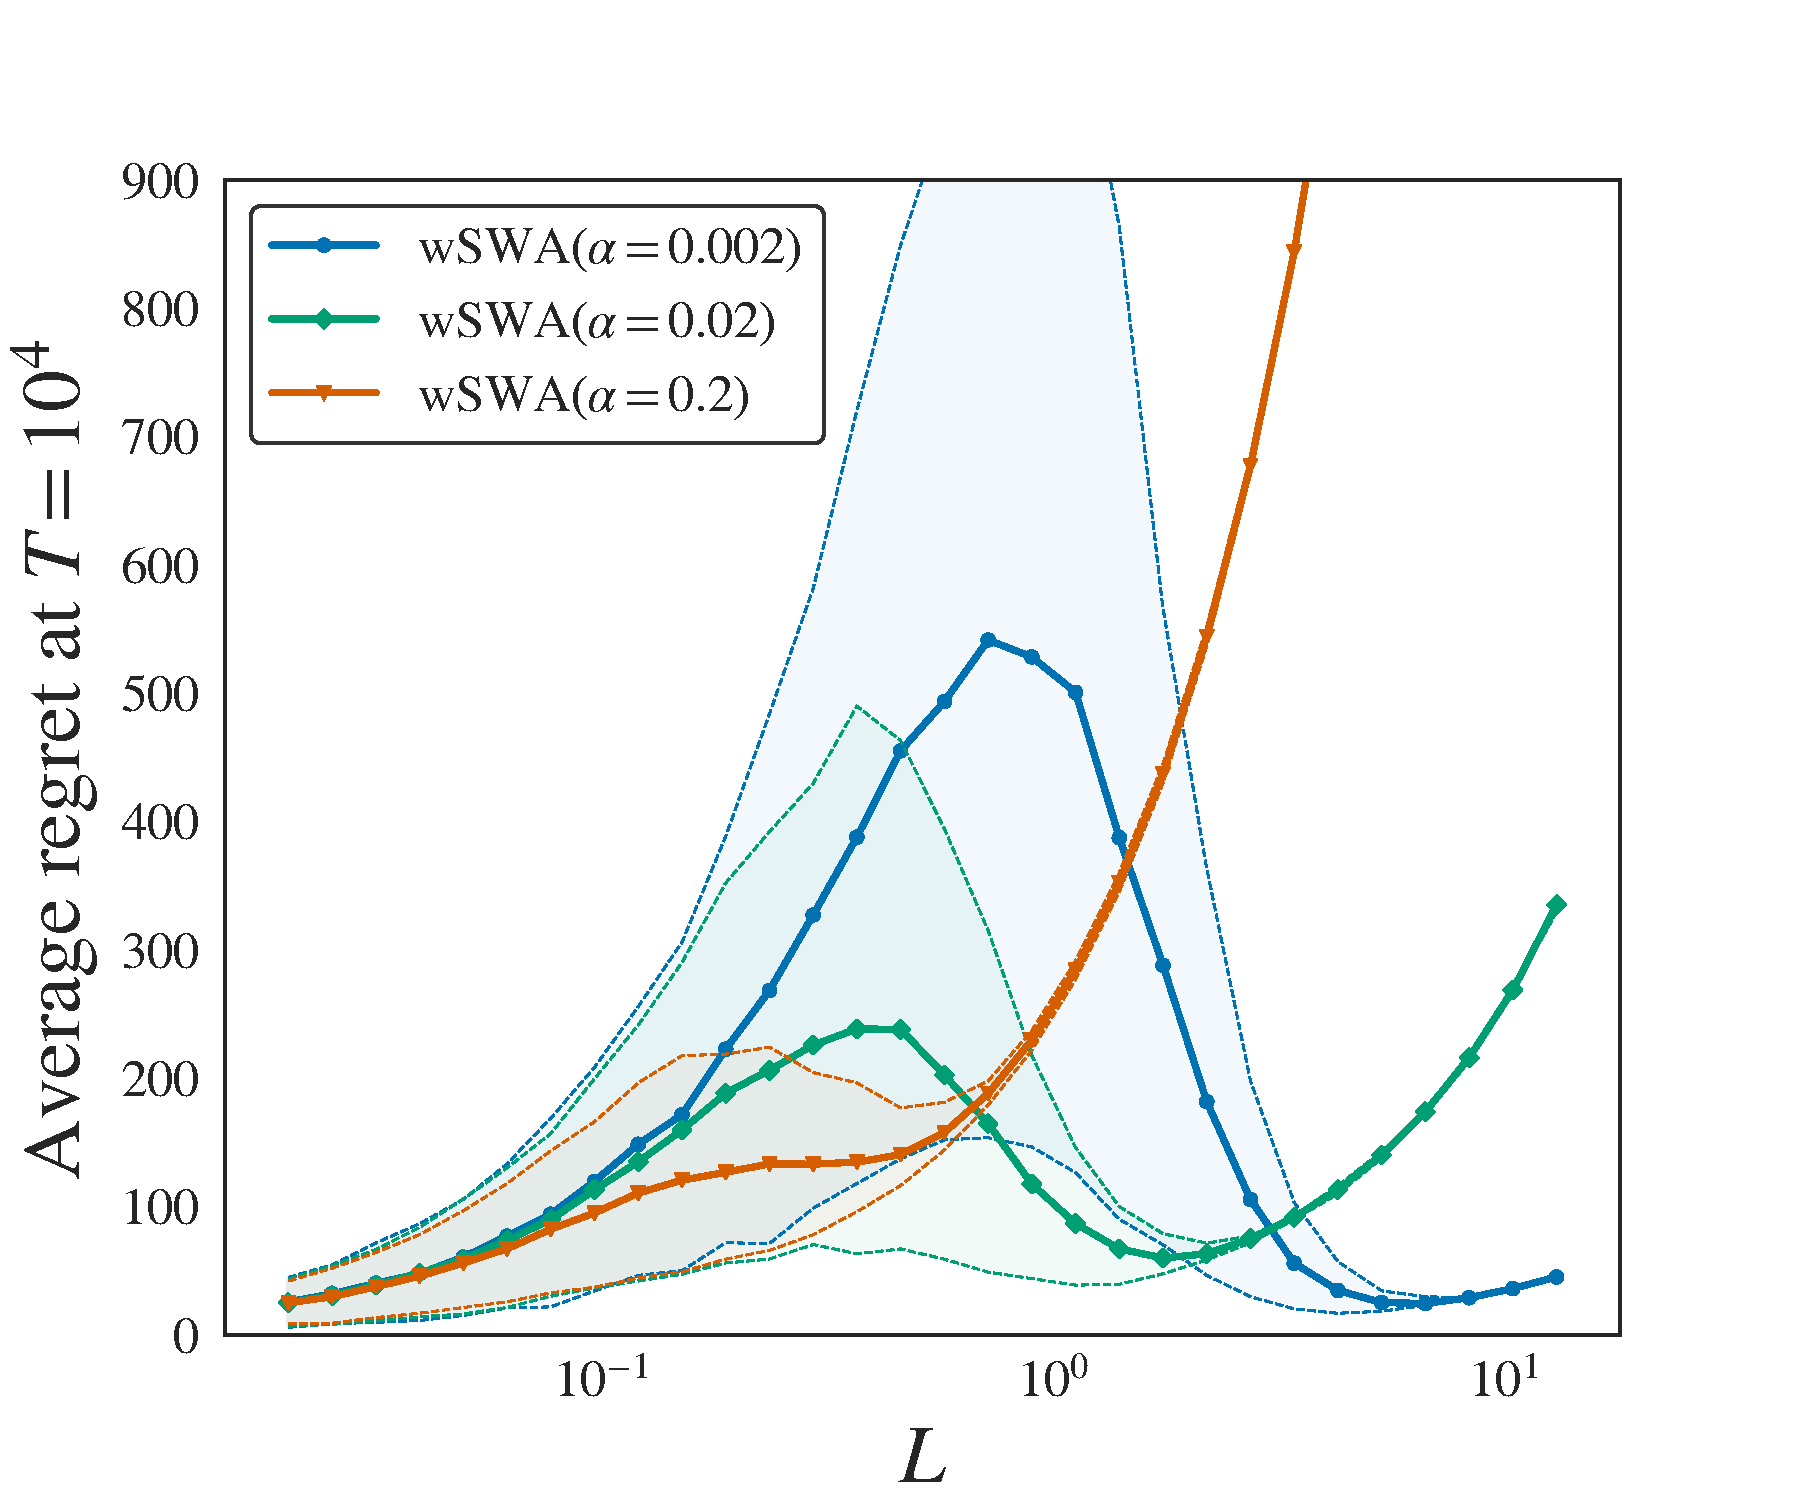
\includegraphics[clip, width= 0.51\textwidth]{2.1Rested/fig/fig1A_SWA.pdf}
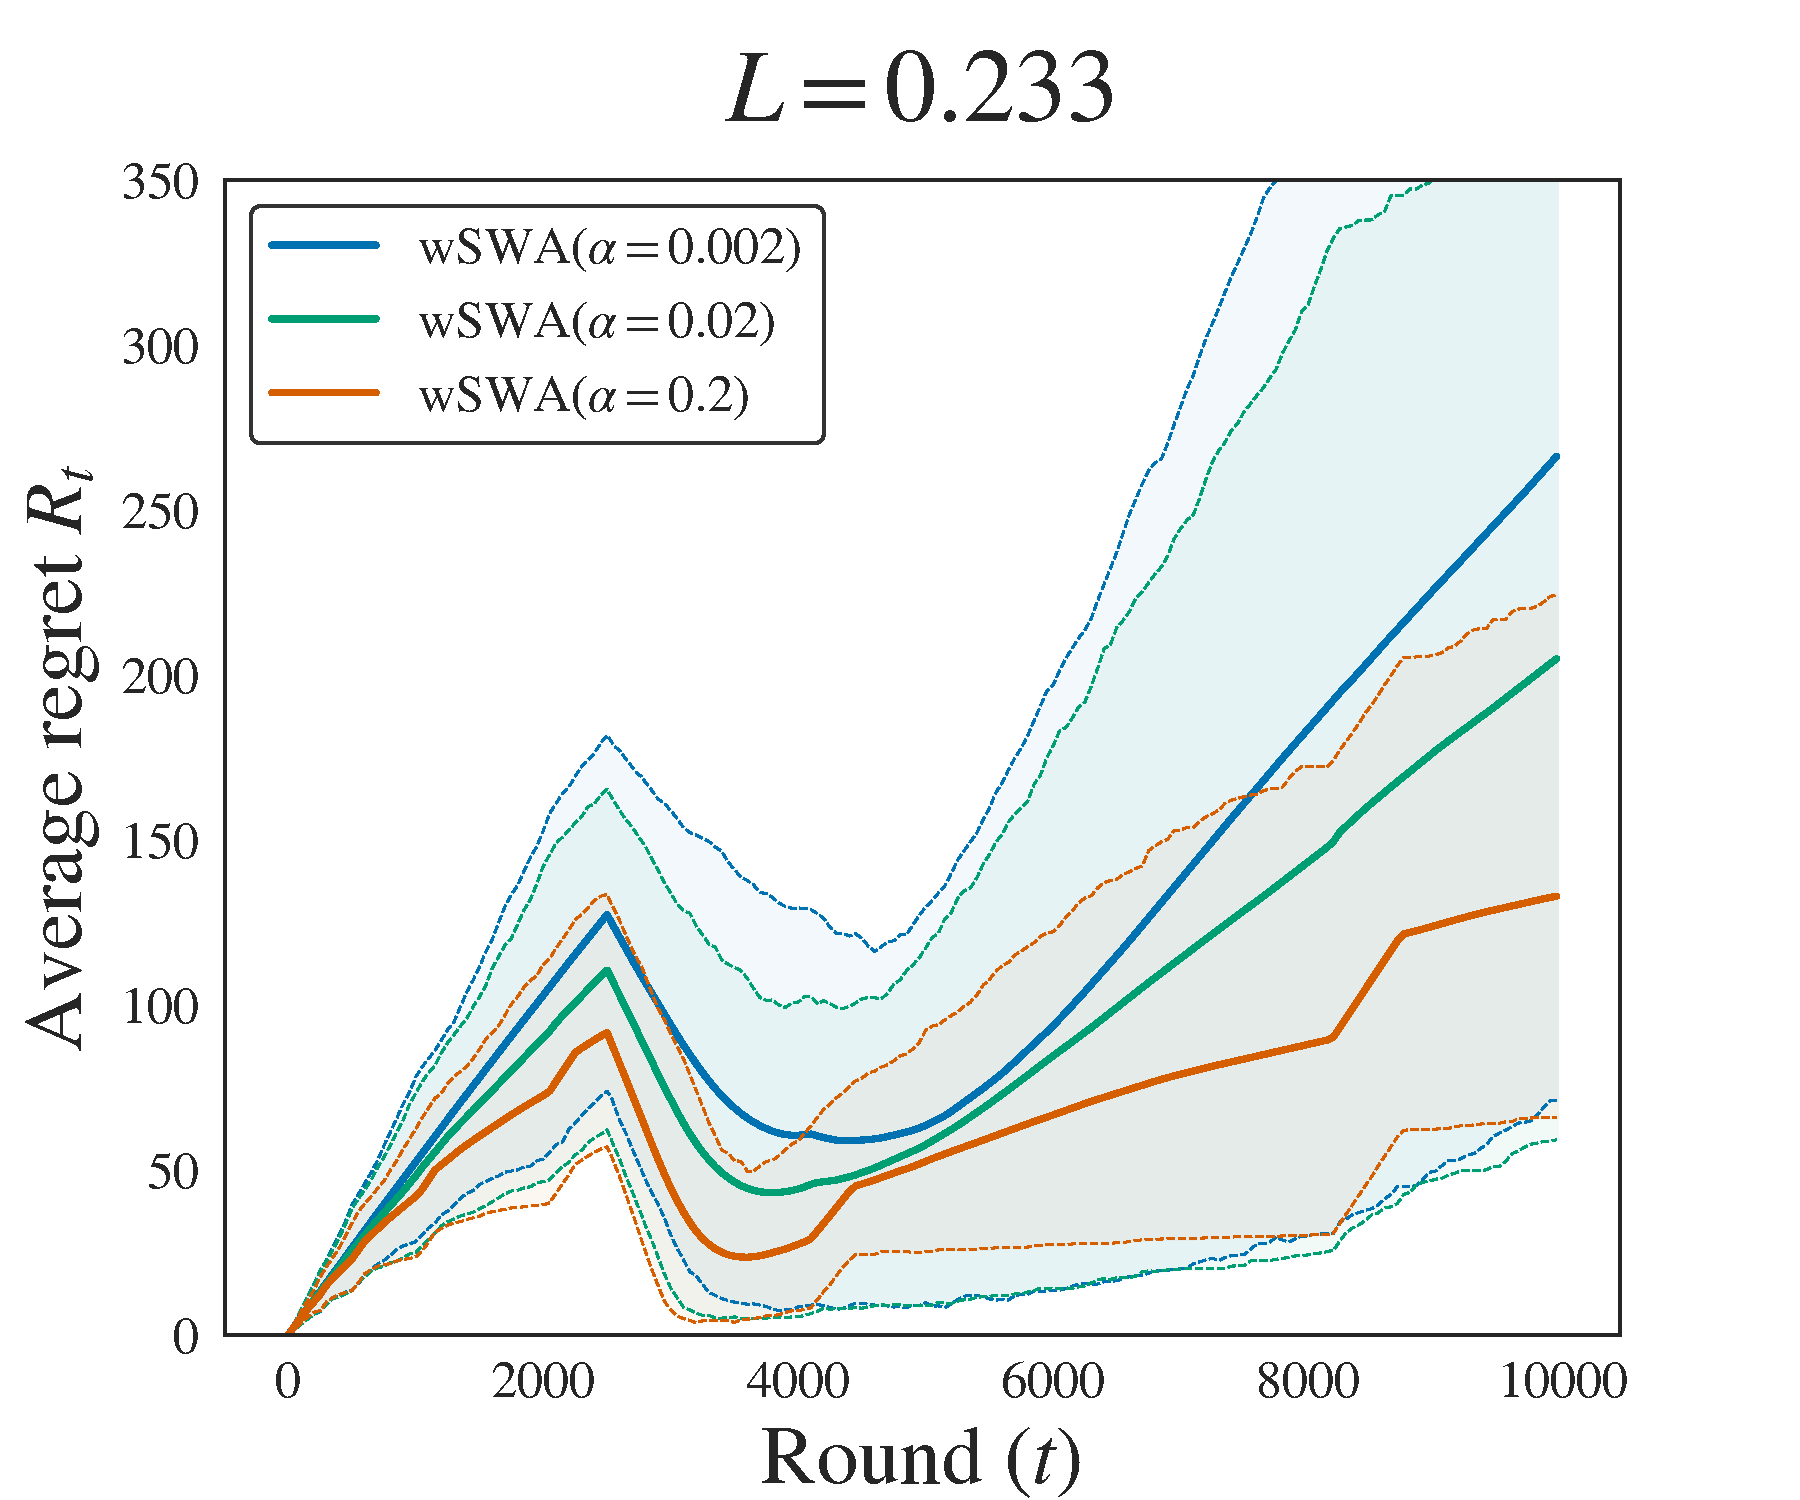
\includegraphics[clip, width= 0.49\textwidth]{2.1Rested/fig/fig1B_SWA.pdf}
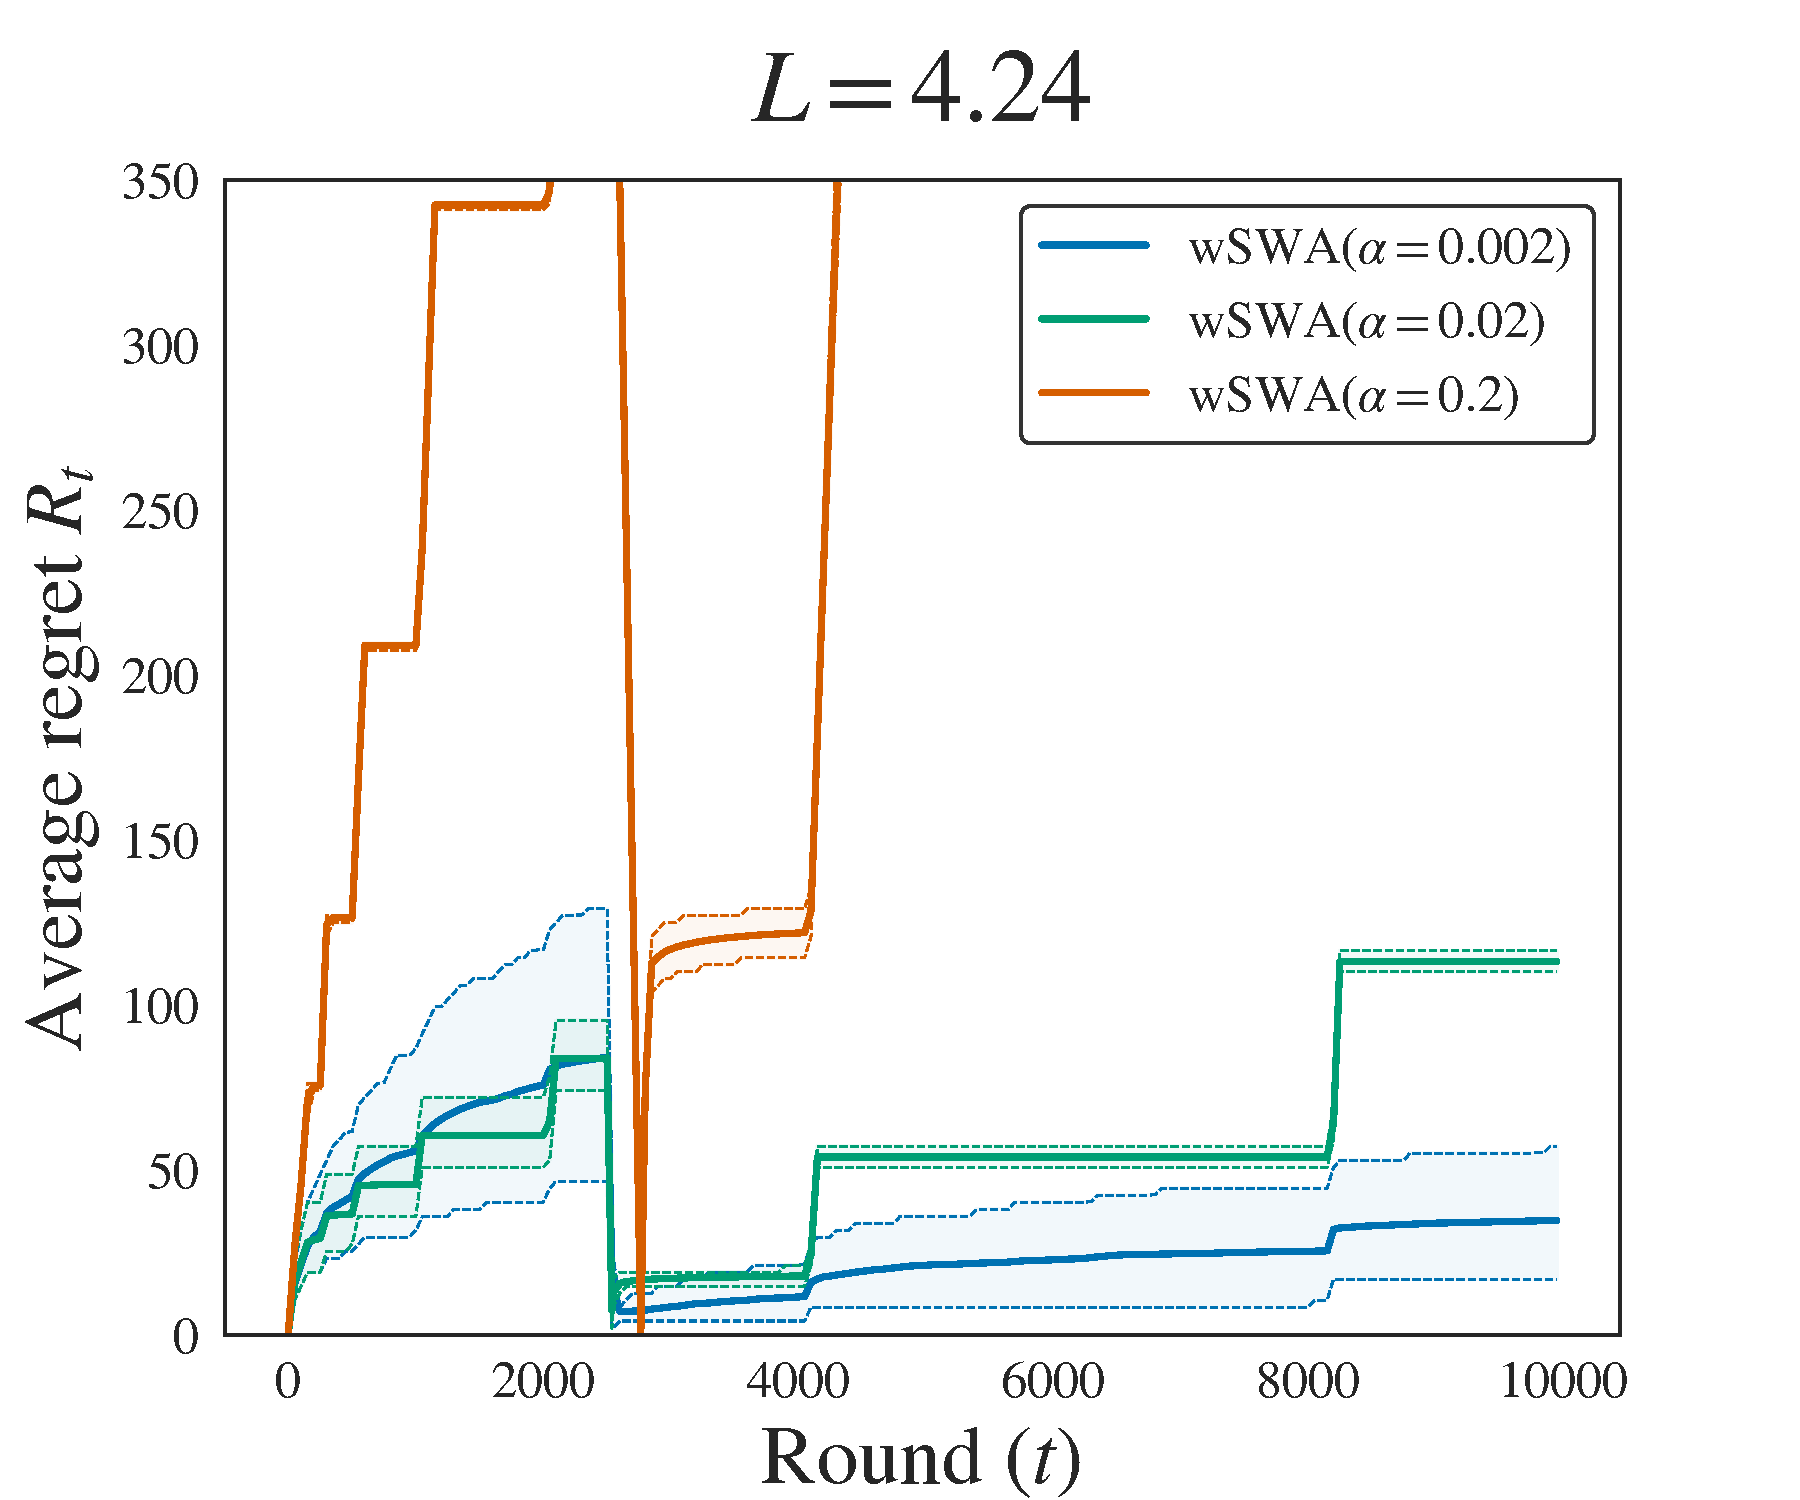
\includegraphics[clip, width= 0.49\textwidth]{2.1Rested/fig/fig1C_SWA.pdf}
\caption{\textbf{Top:} Regret at the end of the game for different values of $L$. \textbf{Bottom:} Regret across time for two values of $L$. Average over 1000 runs. We highlight the $\left[10\%, 90\%\right]$ confidence region.}
\label{fig:SWA1}
\end{figure*}


\paragraph{Results} 
%All experiments are averaged over $1000$ runs.
In Fig.\,\ref{fig:SWA1}, we compare the performance of the three versions of \wSWA. The top plot shows the regret at the last round $T = 10 000$ for 30 different values of~$L$. The bottom plots show the regret as a function of time for $L = 0.233$ and $L=4.24$.  

Each curve of the top plot has three different parts. First, we observe a linear increase for small values of $L$ (exponential shape on the semi-log plot). Indeed, when $\Delta = \nicefrac{L}{2} \lesssim \nicefrac{\sigma}{\sqrt{h}}$, the variance of the indexes are greater than the gap between arms. Therefore, the algorithms are unable to consistently choose the good arm and they do $\cO\pa{T}$ mistakes of size $\Delta$. Hence, the regret grows linearly with $\cO\pa{T\Delta}$ and ultimately with $L$. 

Then, the regret stagnates (red curve) or sharply decreases (green and blue curve). When $\Delta \gtrsim \nicefrac{\sigma}{\sqrt{h}}$, the variance of the indexes is smaller than the gap between arms. Hence, the number of mistakes decrease at an exponential rate with $L^2$ (according to Hoeffding inequality) from $\cO\pa{T}$ to $\tcO\pa{h}$. Notice that there is indeed a factor $\sqrt{\nicefrac{\alpha_{blue}}{ \alpha_{green}}} \sim 3$ between the x-coordinate of the green and blue peaks: it matches the order of magnitude of $L_{peak} \sim  \nicefrac{\sigma}{\sqrt{h}}$.

Yet, in this setup, the concentration of the index can only reduce the number of overpulls of arm $2$ up to $\sim \nicefrac{h}{2}$. Indeed, the expected value of the index of arm $2$ is larger than the expected value of the index of arm $1$ until we do $\nicefrac{h}{2}$ overpulls of arm $2$ because of the bias caused by the pulls before the breakpoint. Moreover, at each restart of the algorithm, both arms are pulled $h$ times. Thus, the regret is lower-bounded by $\tcO\pa{Lh}$ for any $L$ due to the doubling trick restart and the bias of the index. That is why we observe a linear increase (exponential shape on the semi-log plot) of the regret at the end of the green and red curves. Notice that there is a factor 10 between the red and green curves for large values of $L$, which confirms the $\cO\pa{Lh}$ regret rate. We highlight that the red curve does not decrease because this exponential increase takes over the decrease due to the concentration of the index.

The bottom plots show the evolution of the regret for two different values of $L$. We notice that the regret first increases, then decreases at $t = \ceil{\nicefrac{T}{4}}$  and increase again. The regret decreases because at $t = \ceil{\nicefrac{T}{4}}$ the arms' value for the optimal policy are $0$ and $-\nicefrac{L}{2}$  while any sub-optimal policy can obtain either $0$ or $+\nicefrac{L}{2}$. Therefore, the regret cannot increase until \wSWA has pulled arm $2$ for $\floor{\nicefrac{T}{4}}$ times. At this round, the regret is $0$ because we are at the optimal pulling allocation. Notice that we display the expected regret, which might not be equal to $0$ because the different runs do not reach $0$ at the same round.  After that, the regret increases again as \wSWA may select arm $2$ with sub-optimal value $-\nicefrac{L}{2}$.

For $L=0.233$, $\alpha= 0.2$ is the best tuning. Indeed, the difference between arms is only of $\Delta = 0.1$ which is small compared to $\sigma =1$. Therefore, we need a reasonably large averaging window to decrease the variance of the indexes below the gaps between arms, \ie $h \sim \nicefrac{\sigma^2}{\Delta^2} \sim 100$ which is the order of magnitude when $\alpha = 0.2$ ($h=272$ at the end of the game). For $L = 4.24$, $\alpha=0.002$ is the best tuning. Indeed, following the same reasoning, we need $h \sim 1$ which is coherent with $h=3$ at the end of the game when $\alpha = 0.002$.

At each full restart due to the doubling trick wrapper, the two arms are pulled $h$ times which generates $\nicefrac{hL}{2}$ extra regret. The cost of this operation is particularly prohibitive when either $h$ or $L$ is large. For instance, when $L=4.24$, we see periodic sharp increments in the regret when $t=2^i$, especially for the larger values of $\alpha$.


\subsubsection{Simulated benchmark $\#$2: Learning against several drops (10 arms)}
\paragraph{Experiments.} We also tested a rotting setting with 10 arms. The mean of 1 arm is constant with value 0 while the means of 9 arms abruptly decrease after 1000 pulls from $+\Delta_i$ to $-\Delta_i$. We use nine different values of $\Delta_i$ which are ranging from 0.001 to 10 in a geometric sequence. In this setting, the regret can be written as $R_T(\pi) = \sum_{i=1}^9 h_{i,T}\Delta_i$, with $h_{i,T}$ the number of overpulls of arm $i$ at round $T$. We define the regret per arm, $R_T^i(\pi) \triangleq \Delta_i h_{i,T}$.

\paragraph{Algorithms.} We keep the three versions of \wSWA with $\alpha \in \left\{ 0.002, 0.02, 0,2\right\}$. We add to our benchmark famous stationary, adversarial and non-stationary algorithms: \UCB \citep{lai1985asymptotically}, \EXP, \EXPS \citep{auer2002nonstochastic}, \DUCB, \SWUCB \citep{garivier2011upper-confidence-bound} and \GLRUCB \citep{besson2019generalized}. 

For $\UCB$ we use the asymptotic optimal tuning of the confidence bounds for stationary gaussian bandits. For $\EXP$ and $\EXPS$, we use theoretical tuning using the number of breakpoints and the horizon. For \SWUCB and \DUCB, we select the forgetting parameters $\tau=200$ and $\gamma = 0.997$ with grid-search for best performance on this problem. For \GLRUCB, we use the theoretical value $\delta = \sqrt{T}^{-1}$ for the change-point sensitivity and we set the probability of random exploration to $0$. Indeed, the random exploration is used to detect (restless) increment in the sub-optimal arms value which is irrelevant for our rested rotting setup.


\begin{figure*}[t]
\centering
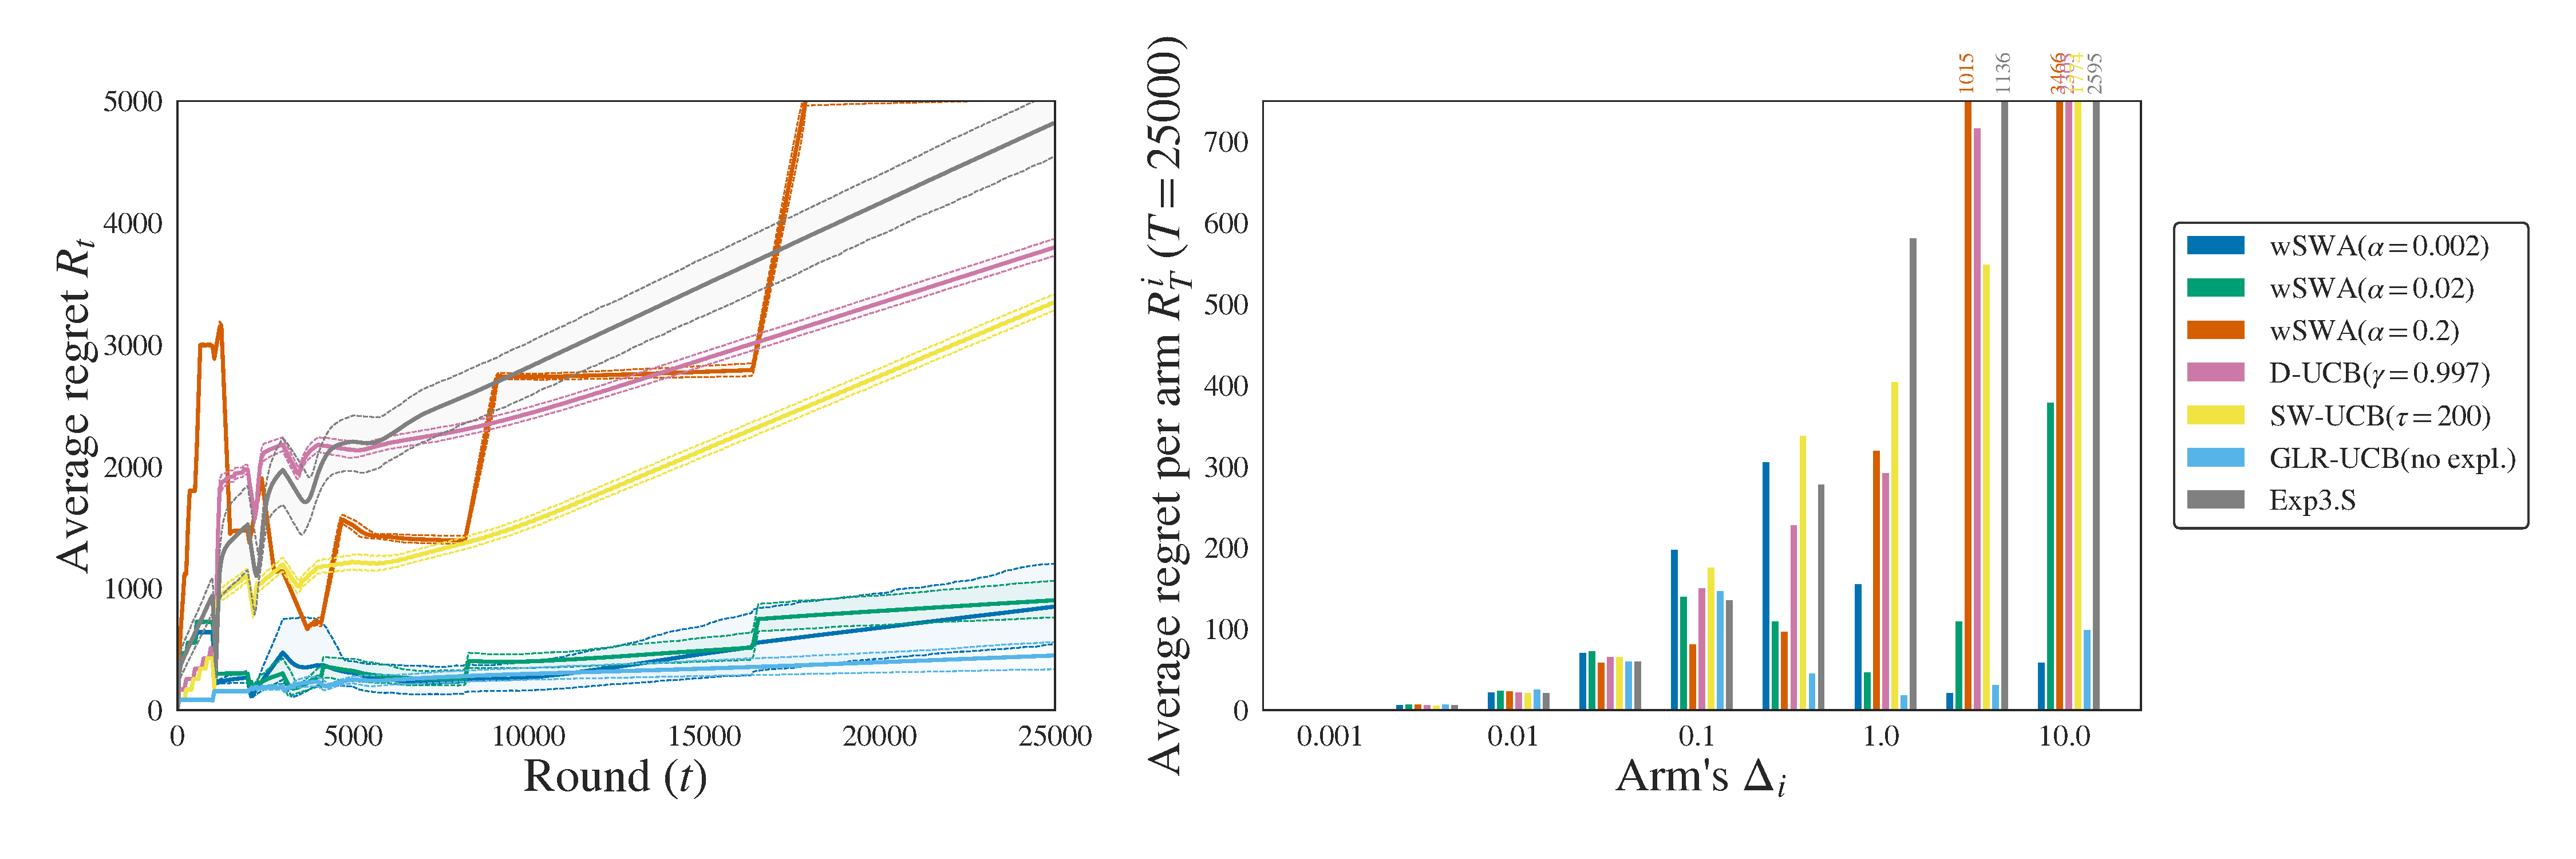
\includegraphics[width = 0.99 \textwidth]{2.1Rested/fig/fig2_SWA.pdf}
\caption{\textbf{Left:} Regret at the end of the game for different values of $L$. \textbf{Middle, Right:} Regret across time for two values of $L$. Average over 1000 runs. We highlight the $\left[10\%, 90\%\right]$ confidence region.}
\label{fig:SWA2}
\end{figure*}

\paragraph{Results.} We display the average regret through the rounds and the regret per arm at the end of the horizon in Figure~\ref{fig:SWA2}.

We do not display the results for \UCB and \EXP because they obtain very large regret after the first drop in the reward (~20 000 at the end of the game). Indeed, these two algorithms are designed for the fixed-arm regret and are unable to adapt to change of the best arm identity. 
 
\SWUCB, \DUCB, and \EXPS show large regret even though \SWUCB and \DUCB were optimally tuned for this problem. These algorithms use random exploration and/or restless forgetting of the data associated with each arm. This is harmful because it leads to multiple pulls of a very suboptimal arm. Yet, with the rested rotting non-stationarity, an identified bad arm has no reason to improve.
 
\SWA shows better performance when it is rightly tuned. In this problem, we have multiple sizes of drops and one should choose a value $\alpha$ which trades-off between these different sizes.  $\alpha=0.2$, which obtains the best value in \citet{levine2017rotting}'s experiment, has a very large regret in our benchmark. Indeed, the best tuning depends on the maximal size of the drops, which is quite large in our setting. We also notice the cost of the doubling trick.

Last, \GLRUCB shows good performance when random exploration is turned off. Indeed, the change detection mechanism reset the history of the arm when there is significant evidence of a change. Hence, the number of mistakes after a drop is adaptive to the difficulty to detect the change. 

\subsection{Open problems}
\label{subsec:rested-open}
\subsubsection{Minimax rate}
We report existing regret bounds for two special cases. First, in Proposition~\ref{prop:lb-noisefree}, \citet{heidari2016tight} show that in the absence of noise, the regret is lower bounded by $\cO\pa{KL}$. Second, we recall the minimax regret lower bound for stochastic stationary bandits.

\begin{proposition}[\cite{auer2002nonstochastic}][Thm.\,5.1]
\label{stochastic-LB}
For any learning policy $\policy$ and any horizon $T$, there exists a stochastic stationary problem $\left\{ \mu_i (n) \triangleq \mu_i\right\}_i$ with $K$ $\sigma$-sub-gaussian arms such that $\pi$ suffers a regret
\begin{equation*}
%\max_{\left\{ \mu_i \in [0,L] \right\}_i}
 \mathbb{E}[\regret(\policy)] \geq \frac{\sigma}{10}\min\pa{\sqrt{\narms\timeEnd},\timeEnd}.
\end{equation*}
where the expectation is w.r.t.\ both the randomization
over rewards and algorithm's internal randomization.
\end{proposition}

Any problem in the two settings above is a rotting problem with parameters ($\sigma$, $L$). Therefore, the performance of any algorithm on the noisy rotting problem is also bounded by these two lower bounds. For reward functions in $\BBSet$, \SWA is guaranteed to achieve $\cO\pa{T^{\nicefrac{2}{3}}}$ regret rate. Yet, \citet{levine2017rotting} do not provide a lower bound while they suggest it could be an interesting future work direction.

\subsubsection{Problem-dependent rate}
\SWA starts by pulling every arm $h$ times. It means that even for simple stationary problem with large difference $\Delta_i > \sigma$ between suboptimal and optimal arms, \SWA makes at least $h = \cO\pa{T^{\nicefrac{2}{3}}}$ mistakes per suboptimal arms which is much more than the stationary asymptotic optimal pulling rate $\cO\pa{\nicefrac{\sigma\log\pa{T}}{\Delta_i^2}}$.


\subsubsection{Agnostic algorithm}
\SWA requires the knowledge of the horizon $T$, the subgaussian parameter $\sigma$, and the reward range $B$  to tune the window $h$. We showed empirically that the doubling trick leads to large regret increases at each restart. We also show that not knowing the amplitude of the drops $B$ could lead to very suboptimal tuning.

\begin{remark}
\citet{levine2017rotting} suggest in \wSWA to use the classical doubling trick, with a full restart of the memory of the algorithm. It is an easy way to generalize the $\tcO\pa{T^{\nicefrac{2}{3}}}$ bound when we do not know $T$. However, in practice, in this rested setup, there is no good reason to clean the memory of \wSWA (see Line~\ref{algline:wSWA-clean}). We could simply increase the window $h$ and keep the current history of the arms in order to diminish the cost of the restart. The empirical investigation of this algorithm showed improved results compared to \wSWA without completely removing the extra cost of the doubling trick.
\end{remark}


\subsubsection{Global budget or Budget per round}

The analysis of \SWA was carried in the global rotting budget setting while the analysis of the noiseless case was carried in the per round budget setting. We can translate the $\tcO\pa{B^{\nicefrac{1}{3}}T^{\nicefrac{2}{3}}}$ bound by setting $B= LT$ which leads to linear regret (see the remark following Definition~\ref{def:rew-bounded}). Hence, no algorithm is proved to achieve a $o(T)$ regret bound in the rotting budget per round setting with noise.

%!TEX root = ../main.tex 
\section{{\FEWA} and {\RAW}: Two adaptive window algorithms}
\label{sec:algo}
%
\subsection{Towards adaptive windows}
Since the expected rewards $\mu_i$ change from one pull to another, the main difficulty in the rested rotting bandits is that we cannot rely on all samples observed until time~$t$ to predict which arm is likely to return the highest reward in the future. In fact, the older a sample, the less representative it is for future rewards. This suggests constructing estimates using more recent samples. Nonetheless, discarding older rewards reduces the number of samples used in the estimates, thus increasing their variance.

In Figure~\ref{fig:SWA1}, we showed different setups in which the regret of \wSWA scales either with $\cO\pa{KLh}$ (for large $L$) or with $\tcO\pa{\nicefrac{T\sigma}{\sqrt{h}}}$ (for small $L$). \wSWA chooses a window $h$ which balances between these two costs. Yet, the two situations are quite different. In Figure~\ref{fig: adaptive_window}, we show three different reward functions with the associated data. The first one has a large decay $L> \sigma$ at the end of the sequence. The second one has a rather small decay in the middle. The last one is stationary. For these three arms, we should probably not use the same window to estimate the three values.

\begin{figure*}[h]
\centering
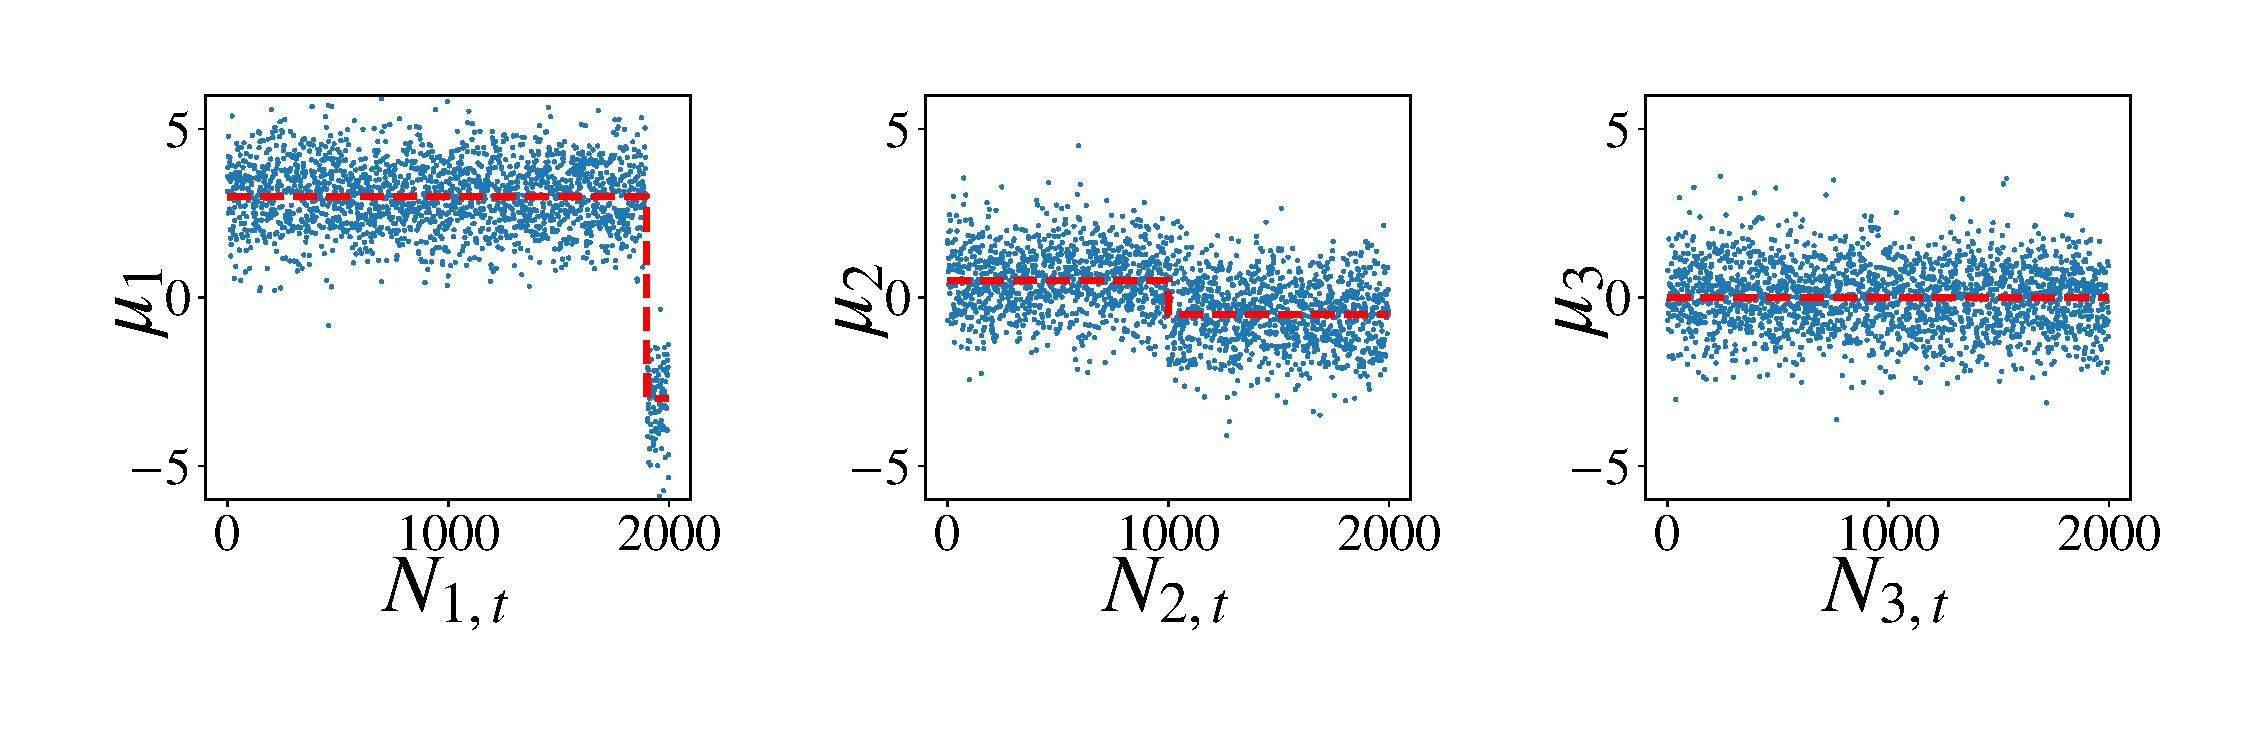
\includegraphics[clip, width= 0.99\textwidth, trim={ 1cm 2cm 1cm 1cm}]{2.1Rested/fig/adaptive_windows.pdf}
\caption{Three rotting reward functions (red dash line) and associated reward samples: Why should we use a single fixed window size to compare these three arms?}
\label{fig: adaptive_window}
\end{figure*}




\paragraph{A favorable event for adaptive windows}
\begin{proposition}
\label{prop:prb_favorable_event}
For any round $t$ and confidence $\delta_{t} \triangleq 2t^{-\alpha}$, let 
%
\begin{equation}
\!\HPevent\! \triangleq\! \Big\{ \forall i\!\in\!\arms,\ \forall n \!\leq\! t\!-\!1 ,\ \forall h \!\leq\! n, \big| \hmu^h_i(t, \pi) - \bmu^h_i(t,\pi) \big| \!\leq\! c(h, \delta_{t}) \!\Big\}
\label{eq:def_favorable_event}
\end{equation}
 be the event under which the estimates at a round $t$  are all accurate up to $c(h,\delta_{t}) \triangleq \sqrt{2 \subgaussian^2\log(2/\delta_t)/h}$. Then, for a policy $\pi$ which pulls each arms once at the beginning, and for all $t>K$,
\[
\PPempty\Big[\bar{\HPevent}\Big] \leq \frac{Kt^2\delta_{t}}{2}=Kt^{2-\alpha}\,.
\]
\end{proposition} 

\begin{proof}
We want to upper bound the probability
\[
\PP{\bar{\HPevent}} = \PP{\exists i \in K,\,\exists n \leq t-1, \exists h \leq\, n, \big|\hmu^h_i(n)-\bmu^h_i(n)\big|>c(h,\delta_t) }.
\]

Following the same argument as in Proposition~\ref{prop:prb_favorable_event_SWA}, there exists a sequence of random independent variable $(\epsilon'_l)_{l\in\NN}$ , $\sigma^2$ sub-Gaussian such that for $\hepsilon^h_n \triangleq (1/h) \sum_{l=n-h+1}^n \epsilon'_l$ we get, 
\begin{align*}
    \PPv\Big[\exists n \leq t-1, \exists h &\leq\, n, \big|\hmu^h_i(t-1,\pi)-\bmu^h_i(t-1,\pi)\big|>c(h,\delta_t) \Big]\\
    &= \PP{\,\exists n \leq t-1, \exists h \leq n,\, |\hepsilon^h_n|>c(h,\delta_t) }\\
    &\leq \sum_{n=1}^{t-1}\sum_{h=1}^n \PP{|\hepsilon^h_n|>c(h,\delta_t)} \\
    &\leq  \frac{t(t-1)}{2}\cdot \delta_t \,,
\end{align*}
where we used the Chernoff inequality in the last line. Thus, a union bound  over the arms allows us to conclude that
\[
\PPempty \Big[\bar{\HPevent}\Big]\leq \frac{K \delta_t t^2}{2}\cdot
\]
\end{proof}
\begin{remark}
Compared to the unique favorable event we used for \SWA (see Equation~\ref{eq:def_favorable_event_SWA}), we use a favorable event for each round $t$. It will be helpful to obtain anytime guarantees for our algorithms. Moreover, $\HPevent$ control the deviation of any statistic $\hmu_i^h(n)$ for any possible $h$, $i$ and $n$. This is different from $\HPSWA$ which uses a fixed $h$. 
\end{remark}

\subsection{{\FEWA}: Filtering on expanding window average}
\label{ss:fewa}
In Alg.\,\ref{alg:FEWA}, we introduce \FEWA (or~$\piF$) that at each round $t$, relies on estimates using windows of increasing length to filter out arms that are sub-optimal with high probability and then pulls the least pulled arm among the remaining arms. 
 \begin{figure*}[!ht]
 \begin{minipage}{\textwidth}
\renewcommand*\footnoterule{}
\begin{savenotes}
\begin{algorithm}[H]
\caption{{\FEWA}}
\label{alg:FEWA}
\begin{algorithmic}[1]
\Require $\arms$,  $\subgaussian$, $\alpha$
\For{$t \gets 1, 2, \dots, K \do $}{\footnotesize \Comment{\emph{Pull each arm once}}}
	\State \textsc{Pull}  $i_t \gets t$; \textsc{Receive} $o_{t}$
	\State $N_{i_t} \gets 1$
	\State $\left\{\hmu_{i_t}^h\right\}_h \gets \UPDATE(\left\{\hmu_{i_t}^h\right\}_h, o_t)$\label{algline:fewa-update1}
\EndFor
\For{$t \gets K+1, K+2, \dots \do $}
	\State $h\leftarrow 1$ 
	{\footnotesize \Comment{\emph{initialize bandwidth}}}
	\State $\arms_1 \leftarrow \arms$ 
	{\footnotesize \Comment{\emph{initialize with all the arms}}}
	\State $i_t \gets {\tt none}$
	\While{$i_t$ is  ${\tt none}$} \label{algline:fewa-while}
		\State $\arms_{h+1} \leftarrow {\FILTER}(\arms_{h} ,h, \alpha, \sigma, t)$ \label{algline:fewa-filter}
		\State $h \leftarrow h + 1$ \label{algline:fewa-window}
		\If{$\exists i \in \arms_{h}$ such that $N_{i}=h$}
			\label{algline:fewa-condition}
			\State \textsc{Pull}\footnote{One can choose the tie break selection rule arbitrarily, e.g. by selecting the arm with the smallest index.}  $i_t \in \left\{ i \in \arms_h | N_{i_t} = h \right\}$; \textsc{Receive} $o_{t}$\label{algline:fewa-pull}
		\EndIf
	\EndWhile
    \State $N_{i_t} \leftarrow N_{i_t} +1$
	\State $\left\{\hmu_{i_t}^h\right\}_h \gets \UPDATE(\left\{\hmu_{i_t}^h\right\}_h, o_t)$\label{algline:fewa-update2}
\EndFor
\end{algorithmic}
\end{algorithm}
\end{savenotes}
\end{minipage}
\end{figure*}

We first describe the subroutine {\FILTER} in Alg.\,\ref{alg:filter}, which receives a set of active arms $\arms_h$, a window~$h$, a confidence bound tuning parameter $\alpha$ and the subgaussian parameter $\sigma$  as input and returns an updated set of arms $\arms_{h+1}$. For each arm~$i \in \arms_h$ (that has all been pulled~$n \geq h$ times), the algorithm has stored an estimate $\hmu_i^h$ that averages the $h$ most recent rewards observed from~$i$. 
The subroutine \FILTER discards all the arms whose mean estimate (built with window~$h$) from $\arms_h$  is lower than the empirically best arm by more than twice a threshold $c(h, \delta_t)$ constructed by standard Hoeffding's concentration inequality (see Prop.\,\ref{prop:prb_favorable_event}).



\begin{algorithm}[!ht]
\caption{{\FILTER}}
\label{alg:filter}
\begin{algorithmic}[1]
\Require $\arms_{h}$, $h$, $\alpha$, $\sigma$, $t$
\State $c(h, \delta_t) \leftarrow \sqrt{2\alpha\sigma^2\log{(t)}/h }$
\State $\hmu^h_{\max}  \leftarrow \max_{i \in \arms_{h}}\hmu_i^h$\label{algline:filter-max}
\For{$ i \in \arms_{h}$}
	\State $\Delta_i \leftarrow  \hmu^h_{\max} - \hmu^h_{i} $ \label{algline:filter-delta}
	\If{$\Delta_i \leq 2c(h,  \delta_t) $}
	\State add $i$ to $\arms_{h+1}$ \label{algline:filter-add}
	\EndIf
\EndFor
\Ensure $\arms_{h+1}$
\end{algorithmic}
\end{algorithm}



The \FILTER subroutine is used in \FEWA to incrementally refine the set of active arms, starting with a window of size $1$, until the condition at Line~\ref{algline:fewa-condition} is met. As a result, $\arms_{h+1}$ only contains arms that passed the filter for all windows from $1$ up to $h$. Notice that it is important to start filtering arms from a small window and to keep refining the previous set of active arms. 
In fact, the estimates constructed using a small window use recent rewards, which are closer to the future value of an arm. As a result, if there is enough evidence that an arm is suboptimal already at a small window $h$, it should be directly discarded. On the other hand, a sub-optimal arm may pass the filter for small windows as the threshold $c(h , \delta_t)$ is large for small $h$ (i.e., because a few samples are used in constructing $\hmu_i^h$, the estimation error may be high). Thus, \FEWA keeps refining $\arms_{h}$ for larger windows in the attempt of constructing more accurate estimates and discard more sub-optimal arms. This process stops when we reach a window as large as the number of samples for at least one arm in the active set $\arms_{h}$ (i.e., Line~\ref{algline:fewa-condition}). At this point, increasing $h$ would not bring any additional evidence that could refine $\arms_{h}$ further (recall that $\hmu^h_i$ is not defined for $h > N_i$). Finally,  \FEWA selects the active arm $i_t$ whose number of samples matches the current window, i.e., the least pulled arm in $\arms_{h}$. The set of available rewards and the number of pulls are then updated accordingly. 

\paragraph{Core guarantee on the favorable event} 
We derive an important lemma that provides support for the arm selection process obtained by a series of refinements through the \FILTER subroutine. Recall that at any round $t$, after pulling arms $\{ \Nitmone\}_i$ the greedy (oracle) policy would select an arm 
%
\begin{align*}
i^\star_t \pa{\left\{ \Nitmone \right\}_i}  \in  \argmax_{i \in \arms} \mu_i \left( \Nitmone\right).
\end{align*}
%
We recall that $\mu^+_t(\piF) \triangleq \max_{i \in \arms} \mu_i (\Nitmone)$ the reward that could be obtained by pulling~$i^\star_t$ at a round $t$. 
While \FEWA cannot directly match the performance of the oracle arm, the following lemma guarantees that the past performance of the selected arm is close enough compared to the current best arm value. 

\begin{restatable}{lemma}{restalemmafewa}
\label{lem:core-FEWA}
For {\FEWA} tuned with $\alpha$, on the favorable event $\HPevent$, if an arm~$i$ passes through a filter of window $h$ at a round $t$, i.e., $i\in\ \arms_h$, then the average of its $h$ last pulls satisfies
%
\begin{equation}\label{eq:fundamental-eq-FEWA}
\bmu^{h}_i(\Nitmone ) \geq  \mu^+_t(\piF) - 4 c(h, \delta_t).
\end{equation}
Therefore, at a round $t$, on favorable event $\HPevent$, if arm~$i$ is selected by {\FEWA($\alpha$)}, for any $h \leq \Nitmone$,  the average of its $h$ last pulls cannot deviate significantly from the best available arm at that round, i.e.,
%
\begin{equation*}
\bar{\mu}^{h}_{i_{t}}(\Nitmone) \geq \mu^+_t(\piF) - 4 c(h, \delta_{t}).
\end{equation*}
\end{restatable}

\begin{proof}
We will prove this property for a more general rotting feedback model than the rested rotting one presented in Equation~\ref{eq:rested-feedback}. We will use this more general proof in the next Chapter~\ref{ch:restless}. If arm $i$ is selected at the round $t$, the learner $\pi$ receives,
\[
o_t \triangleq \mu_{i, \, t} + \noise_t  \;\; \text{with}\; \EE{ \noise_t | \historyt }= 0 \;\; \text{and} \; \forall \lambda \in \R, \; \EE{ e^{\lambda\noise_t}} \leq e^{\frac{\subgaussian\lambda^2}{2}},
\]
with $\left\{ \mu_{i, \, t}\right\}_{t\leq T}$ a non-increasing sequence. We do not specify how the reward is rotting, while it was assumed in Equation~\ref{eq:rested-feedback} that the reward function was evolving with the number of pulls $\Nitmone$ of arm $i$ at the round $t$. With this reward model, we cannot use $\bmu^{h}_{i}(\Nitmone^{\pi})$ to refer to $\bmu_i^h(t,\pi)$, the average of the $h$ last means associated to arm $i$ (see the definition in Equation~\ref{eq:def-bmu} and the following remark). We also extend the definitions of $i_t^\star \in \argmax_{i\in \arms} \mu_{i,t}$ and $\mu_t^+ \triangleq \max_{i \in \arms} \mu_i(N_{i,t-1})$.

Let $i \in \arms_h$ be an arm that passed a filter of window $h$ at the round $t$.
First, we use the confidence bound for the estimates and we pay the cost of keeping all the arms up to a distance $2c(h,  \delta_t)$ of $\hmu^{h}_{\max,\, t} \triangleq \max_{j \in \arms_h} \hmu_i^h(t,\piF)$,
\begin{equation}
\label{1}
\bmu_i^h(t,\piF)\geq \hmu_i^h(t,\piF)- c(h,  \delta_t) \geq \hmu^h_{\max,t} - 3c(h, \delta_t)
\geq \max_{j \in \arms_h}\bmu_j^h(t,\piF)  - 4 c(h, \delta_t),
\end{equation}
where in the last inequality, we used that for all $j \in \arms_h,$ \[\hmu^{h}_{\max,t} \geq  \hmu_j^h(t,\piF)  \geq \bmu_j^h(t,\piF)  - c(h, \delta_t).\]
Second, we call $t_{i,t} < t$ the last round at which arm $i$ was selected. Since the means of arms are decaying, we know that 
\begin{align}
\label{2}
 \mu^+_t(\piF) &\triangleq \mu_{i^\star_t, \, t} \nonumber\\
 &\leq  \mu_{i^\star_t, \, t_{i,t}} =  \bmu_{i^\star_t}^1(t,\piF)  \nonumber\\
 &\leq \max_{j \in \arms}\bmu_j^1(t,\piF)  = \max_{j \in \arms_1} \bmu_j^1(t,\piF).
\end{align}
Third, we show that the largest average of the last $h'$ means of arms in $\arms_{h'}$ is increasing with~$h'$,
\begin{equation*}
\forall  h' \leq h ,  \max_{j \in \arms_{h'+1}}\bmu_j^{h'+1}(t,\piF)   \geq \max_{j \in \arms_{h'}}\bmu_j^{h'}(t,\piF). 
\end{equation*}
To show the above property, we remark that thanks to our selection rule, the arm that has the largest average of means, always passes the filter. Formally, we show that $\argmax_{j \in \arms_{h'}}\bmu_j^{h'}(t,\piF) \subseteq \arms_{h'+1}.$ 
Let $i^{h'}_{\max} \in \argmax_{j \in \arms_{h'}}\bmu_j^{h'}(t,\piF)$. Then, for such $i^{h'}_{\max}$, we have
\begin{equation*}
\hmu_{i^{h'}_{\max}}^{h'}(t,\piF) \geq \bmu_{i^{h'}_{\max}}^{h'}(t,\piF) - c(h', \delta_t) 
\geq \bmu^{h'}_{\max,t} - c(h', \delta_t) \geq \hmu^{h'}_{\max,t}- 2c(h', \delta_t),
\end{equation*}
where the first and the third inequality are due to concentration of the estimates on $\HPevent$, while the second one is due to the definition of $i^{h'}_{\max}$. 

Since the arms are decaying, the average of the last $h' +1$ mean values for a given arm is always greater than the average of the last $h'$ mean values
and therefore, 
\begin{equation}
\label{3}
 \max_{j \in \arms_{h'}}\bmu_j^{h'}(t,\piF) =   \bmu_{i^{h'}_{\max}}^{h'}(t,\piF) \leq \bmu_{i^{h'}_{\max}}^{h'+1}(t,\piF) \leq \max_{j \in \arms_{h'+1}}\bmu^{h' +1 }_{j}(t,\piF), 
\end{equation}
because $i^{h'}_{\rm max} \in \arms_{h'+1}$. Gathering Equations~\ref{1}, \ref{2}, and~\ref{3} leads to the first claim of the lemma,
\begin{align*}
\bmu^{h}_i(t,\piF)
&\stackrel{\eqref{1}}{\geq} \max_{j \in \arms_h}\bmu^{h}_{j}(t,\piF) - 4c(h, \delta_t)\\
&\stackrel{\eqref{3}}{\geq} \max_{j \in \arms_1}\bmu^{1}_{j}(t,\piF)- 4c(h,  \delta_t)\\
&\stackrel{\eqref{2}}{\geq}  \mu^+_t(\piF) - 4c(h, \delta_t).
\end{align*}
To conclude, we remark that if $i$ is pulled at the round $t$, then by the condition at Line~\ref{algline:fewa-condition} of Algorithm~\ref{alg:FEWA}, it means that $i$ passes through all the filters from $h=1$ up to $\Nitmone$. Therefore, for all $h\leq \Nitmone$,
%
\begin{equation}
\bmu^{h}_i(t,\piF) \geq  \mu^+_t(\piF) - 4 c(h, \delta_t).
\end{equation}
\end{proof}

\subsection{{\RUCB}: Rotting Adaptive Window Upper Confidence Bound}
\label{ss:rawucb}

 \begin{minipage}{\textwidth}
\renewcommand*\footnoterule{}
\begin{savenotes}
\begin{algorithm}[H]
\caption{{\RUCB}}
\label{alg:RAWUCB}
\begin{algorithmic}[1]
\Require $\arms$,  $\subgaussian$, $\alpha$
\For{$t \gets 1, 2, \dots, K \do $}{\footnotesize \Comment{\emph{Pull each arm once}}}
	\State \textsc{Pull}  $i_t \gets t$; \textsc{Receive} $o_{t}$
	\State $N_{i_t} \gets 1$
	\State $\left\{\hmu_{i_t}^h\right\}_h \gets \UPDATE(\left\{\hmu_{i_t}^h\right\}_h, o_t)$ \label{algline:raw-update1}
\EndFor
\For{$t \gets K+1, K+2, \dots \do $}
	\State \textsc{Pull} \footnote{One can choose the tie break selection rule arbitrarily, e.g. by selecting the arm with the smallest index.} $i_t \in \argmax_i \min_{h \leq N_{i}}\pa{\hmu_i^h + c(h, \delta_t)} $; \textsc{Receive} $o_{t}${\footnotesize \Comment{\emph{cf.\,\eqref{eq:raw_index}}}}; \label{algline:raw-pull}
	\State  $N_{i_t} \gets N_{i_t} +1$
	\State $\left\{\hmu_{i_t}^h\right\}_h \gets \UPDATE(\left\{\hmu_{i_t}^h\right\}_h, o_t)$\label{algline:raw-update2}
\EndFor
\end{algorithmic}
\end{algorithm}
\end{savenotes}
\end{minipage}



We will study a single class of policies which select at each round $t$ the arm with the maximal index of the form
\begin{align}
\label{eq:raw_index}
\operatorname{ind}(i,t, \delta_{t}) \triangleq \min_{h\leq N_{i,t-1}}\pa{ {\hmu}_i^h(\Nitmone) + c(h,\delta_{t})}\quad \text{ with } \; \delta_{t} \triangleq \frac{2}{t^\alpha} .
\end{align}
We set and call this algorithm Rotting Adaptive Window UCB (\RUCB). There is a bias-variance trade-off for the window choice: more variance for smaller sizes of the window $h$ and more bias for larger $h$. The goal of \RUCB is to adaptively select the right window to compute the tightest UCB. \RUCB uses the indexes of \UCBone computed on all the slices of each arm's history which include the last pull. When the rewards are rotting, all these indexes are upper confidence bounds on the \textit{next value}.  Thus, \RUCB simply selects the tightest (minimum) one as the index of the arm: it is a pure UCB-index algorithm. By contrast, when the reward can increase, the learner can only derive upper-confidence bound on past values which are loosely related to the next value. Hence, all the UCB-index algorithms in the restless non-stationary literature need to add change-detection sub-routine, active random exploration, or passive forgetting mechanism. 

\paragraph{Core guarantee on the favorable event}

\begin{restatable}{lemma}{restalemmaraw}
\label{lem:core-RAWUCB}
At the round $t$, on favorable event $\HPevent$, if arm~$i_{t}$ is selected by \RUCB($\alpha$), for any $h \leq N_{i_t,t-1}$,  the average of its $h$ last pulls cannot deviate significantly from the best available arm at that round, i.e.,
%
\begin{equation*}
\bar{\mu}_{i_t}^{h}(N_{i_t,\, t-1}) \geq \max_{i \in \arms} \mu_{i}(\Nitmone) - 2 c(h, \delta_t)\,.
\end{equation*}
\end{restatable}
This lemma is comparable with Lemma~\ref{lem:core-FEWA} about the algorithm \FEWA. Yet, \RUCB has tighter guarantees than \FEWA (2 versus 4 confidence bands), which is the benefit of upper confidence bounds index policies over confidence bound filtering policies. 

\begin{proof}
Like for Lemma~\ref{lem:core-FEWA} (see its proof), our proof is done in a more general rotting framework that can be used in the next chapter. 

We denote by $
i^\star_t \in \argmax_{i\in \possibleArms}{\mu_{i,t}}
$, a best available arm at time $t$ and 
\[
h_{i,t}^{\min} \in \argmin_{h\leq \Nitmone }{\hat{\mu}_i^h(t,\pi) + c(h,\delta_t)},
\]
a window which minimizes \RAWUCB index at time $t$ for arm $i$. Hence, because the reward functions are non-increasing, we know that 
\begin{equation*}
 \mu_{i^\star_t, t } \leq   \bar{\mu}_{i^\star_t}^1(t,\pi) \leq \cdots \leq  \bar{\mu}_{i^\star_t}^{h_{i^\star_t,t}^{\min}}(t,\pi)\cdot
\end{equation*}
On the high-probability event $\xi_t$, we know that the true average of the means cannot deviate significantly from the average of the observed quantity,
\begin{equation*}
\bar{\mu}_{i^\star_t}^{h_{i^\star_t,t}^{\min}}(t, \pi) \leq \hat{\mu}_{i^\star_t}^{h_{i^\star_t,t}^{\min}}(t,\pi) + c(h_{i^\star_t,t}^{\min},\delta_t)\,.
\end{equation*}
We know that the selected arm $i_t$ at time $t$ has the largest index, hence, 
\[
\hat{\mu}_{i^\star_t}^{h^{\min}_{i^\star_t,t}}(t, \pi) + c(h^{\min}_{i^\star_t,t},\delta_t) \leq \hat{\mu}_{i_t}^{h^{\min}_{i_t,t}}(t, \pi) + c(h^{\min}_{i_t,t},\delta_t).
\]
From $h_{i,t}^{\min}$ definition, we know that this quantity is below any upper-confidence bound for any other window $h$
\[
\hat{\mu}_{i_t}^{h^{\min}_{i_t,t}}(t, \pi) + c(h^{\min}_{i_t,t},\delta_t) \leq \hat{\mu}_{i_t}^{h}(t, \pi) + c(h,\delta_t).
\]
Finally, using again the concentration of the average on the $\HPevent$, 
\[
\hat{\mu}_{i_t}^{h}(t, \pi) + c(h,\delta_t) \leq \bar{\mu}_{i_t}^{h}(t, \pi) + 2c(h,\delta_t)\,.
\]
Hence, putting all the equations together, we can write
\begin{equation*}
\bar{\mu}_{i_t}^{h}(t, \pi) \geq \max_{i \in \possibleArms} \mu_{i}(t,N_{i,t-1}) - 2 c(\window, \delta_t).
\end{equation*}
\end{proof}
%!TEX root = ../main.tex 
\section{Regret Analysis}\label{sec:theory}

In the last section, we presented two algorithms which have very different behaviours. Yet, they show two main similarities. First, for each arm they compute several statistics $\hmu_i^h(\Nitmone)$ for different windows $h\leq \Nitmone$. Second, on the same favorable events $\HPevent$ (on which all these aforementioned statistics are well concentrated around their means, see Prop.~\ref{prop:prb_favorable_event}), we have shown that both algorithms share a guarantee with similar shape that we restate in a general form,
\begin{corollary}[Lemmas~\ref{lem:core-FEWA} and~\ref{lem:core-RAWUCB}]
\label{cor:core-RAW-FEWA}
At a round $t$, on favorable event $\HPevent$, if arm~$i_{t}$ is selected by $\pi(\alpha) \in \left\{ \piR, \piF\right\}$, for any $h \leq N_{i_t,t-1}$,  the average of its $h$ last pulls cannot deviate significantly from the best available arm at that round, i.e.,
%
\begin{multline*}
\bar{\mu}_{i_t}^{h}(N_{i_t,\, t-1}) \geq \max_{i \in \arms} \mu_{i}(\Nitmone) - \frac{C_\pi}{\sqrt{2\alpha}} c(h, \delta_t) = \max_{i \in \arms} \mu_{i}(\Nitmone) - C_\pi \sigma\sqrt{\frac{\log\pa{t}}{h}}\,,\\
\text{with } C_{\piR} = 2\sqrt{2\alpha} \text{ and } C_{\piF} = 4\sqrt{2\alpha}.
\end{multline*}
\end{corollary}

We will see that this Corollary is the only characterization we need in our analysis. We first give problem-independent regret bound for \FEWA and \RUCB and sketch its proof in Subsection~\ref{ss:rested-PI}. Then, we discuss problem-dependent guarantees in Subsection~\ref{ss:rested-PD}. Finally, we give a detailed analysis in Subsection~\ref{ss:rested-proof}.


\subsection{Problem-independent bound}
\label{ss:rested-PI}
\begin{restatable}{theorem}{restaalgoindepub}
\label{th:rested-PI}
For any rotting bandit scenario with means $\{\mu_i\}_{i} \in \rewardSet^K$ and any time horizon $T$, $\pi \in \left\{\piR, \piF \right\}$ run with $\alpha \geq 5$ suffers an expected regret of
\begin{equation*}
\mathbb{E}[\regret(\pi)] \leq C_\pi \sigma \sqrt{\log\pa{T}}\pa{\sqrt{KT} +K} + 3KL\, \;\; \text{with } 
\begin{cases}
C_{\piR} \!=\! 2\sqrt{2\alpha}\\
C_{\piF} \!=\! 4\sqrt{2\alpha}
\end{cases}\!\cdot
\end{equation*}
\end{restatable}
\paragraph{Comparison to \citet{levine2017rotting}} The regret of \SWA is bounded by $\tcO(B^{1/3}K^{1/3} T^{2/3})$ for bounded rotting functions in $\BBSet$. According to Subsection~\ref{subsec:rested-open}, the regret guarantee translate in $\cO(T)$ for rotting functions in $\rewardSet$.  Thus, according to its original analysis, \SWA may not be able to learn for our general setting. On the other hand, we could use \FEWA or \RUCB with rotting functions in $\BBSet$ and recover the same regret bound with $L := B$. In this case, our two algorithms suffer a regret of $\tcO(\sqrt{KT})$, thus significantly improving over \SWA. 

The improvement is mostly because \FEWA and \RUCB use adaptive window mechanisms to smoothly track changes in the value of each arm.  Indeed, \SWA relies on a fixed exploratory phase where all arms are pulled in a round-robin way and the tracking is performed using averages constructed with a fixed window. According to Proposition~\ref{prop:SWA}, this fixed window trades off between the cost of biased estimates $\cO\pa{KBh}$ - for scenarios where the arms abruptly decay and their values are overestimated during at most $h$ rounds - and the cost of the variance of estimators $\tcO\pa{{\nicefrac{\sigma T}{\sqrt{h}}}}$ - for scenarios where the arms keep their value close to each other for $\cO\pa{T}$ rounds. In Theorem~\ref{th:rested-PI}, the regret of \FEWA and \RUCB is also bounded by an additive decomposition between the terms depending on the noise level $\sigma$ and the terms depending on the rotting level $L$. Yet, adaptive window algorithms do not need to trade-off: their regret is bounded by $\cO\pa{KL} +\tcO\pa{\sigma\sqrt{KT}}$. It evidence that our algorithms can take decision based on a relevant $h \in \left\{1, \dots, \Nitmone\right\}$ depending on the scenarios.

Last, our algorithms are anytime and agnostic to $L$ (or $B$), while the tuning of \SWA requires to know $B$ and $T$ (or to resort to a doubling trick, which performs poorly in practice). 

\paragraph{Comparison to stationary stochastic bandits}
The regret upper bounds of \FEWA and \RUCB match the worst-case optimal regret bound of the standard stochastic bandits (i.e., $\mu_i(n)$s are constant) up to a logarithmic factor. Whether an algorithm can achieve $\cO(\sqrt{KT})$ regret bound is an open question. On one hand, our analysis needs confidence bounds to hold for different windows at the same time, which requires an additional union bound and thus larger confidence intervals w.r.t.\,\UCBone. On the other hand, our worst-case analysis shows that some of the difficult problems that reach the worst-case bound of Thm.\,\ref{th:rested-PI} are realized with constant functions, which is the standard stochastic bandits, for which \MOSS-like~\citep{audibert2009minimax} algorithms achieve regret guarantees without the $\sqrt{\log T}$ factor. Thus, the necessity of the extra $\sqrt{\log T}$ factor for the worst-case regret of rotting bandits remains an open problem.

\subsection{Problem-dependent bound}
\label{ss:rested-PD}
Since our setting generalizes the stationary stochastic bandit setting, a natural question is whether we pay any price for this generalization. While the result of~\citet{levine2017rotting} suggested that learning in rotting bandits could be more difficult, in Thm.\,\ref{th:rested-PI} we actually proved that \FEWA and \RUCB nearly match the problem-independent regret rate $\tcO(\sqrt{KT})$. We may wonder whether this is true for the \emph{problem-dependent} regret as well.
%
\begin{remark}
Consider a stationary stochastic bandit setting with expected rewards $\{\mu_i\}_i $ and $\mu_\star \triangleq \max_i \mu_i$. For $\pi \in \piFRSet$, on the favorable event $\HPevent$ with $\delta_t \geq 2/T^\alpha$,  we can apply Corollary~\ref{cor:core-RAW-FEWA}  at the last time arm $i$ is pulled (\ie after $\NiT\!-\!1$ pulls) for $h = \NiT\!-\!1$, 
\begin{align}
\mu_\star - \mu_i \leq \frac{C_\pi}{\sqrt{2\alpha}} c\pa{\NiT-1,  \delta_t} = C_\pi\sigma \frac{\sqrt{\log(T)}}{\NiT -1} \CommaBin\nonumber \\
\text{\ or equivalently,\ }
\NiT \leq 1+ \frac{C_\pi^2 \sigma^2 \log(T)}{(\mu_{\star} - \mu_i) ^2}\cdot\label{eq:LaiRob}
\end{align}
Therefore, for $\alpha > 4$\footnote{$\alpha$ should be large enough to control the cost of the unfavorable events, see Lemma~\ref{lem:rested-B}.}, our algorithms match the lower bound of~\citet{lai1985asymptotically} up to a constant factor $C_\pi^2/2$.
\end{remark}
%
With a similar argument, we can show a similar bound on the number of overpulls $\hiT$  of arm $i$ in the general rested rotting bandits case. Indeed, we show in Lemma~\ref{lem:UB-OP-PD} that $\hiT$ is smaller than a problem-dependent quantity $\hiT^+$ which is itself smaller by construction than a function of "gaps" $\Delta_{i,\hiT^+-1}$,
%
\begin{multline}
\label{eq:hit+}
\hiT^+ \triangleq \max \left\{h \in \ev{1, \dots T} |  h \leq 
1 \! + \! \frac{C_\pi^2 \sigma^2 \log \pa{T}}{\Delta_{i,h-1}^2} \right\}\\\text{ with  } \Delta_{i,h} \triangleq \min_{j \in \arms} \mu_j\pa{N_{j,T}^\star \!-\!1} - \bar{\mu}_i^h\left( \NiT^\star \!+\!h \right). 
\end{multline}
\begin{remark}
Notice that for stationary bandits, we have for all $h$, $\Delta_{i,\,h} = \Delta_i = \mu_\star - \mu_i$. In fact, $ \Delta_{i,\,h} $ extends the notion of gap to our non-stationary setting: it is the average gap between the smallest value pulled by the optimal policy and the average value of the $h$ first overpulls of arm $i$.  We also highlight that $\hit^+$ is always defined because $h=1$ always verify the self-bounding property. 
\end{remark}

Moreover,  on the favorable event $\HPevent$, we can show that the regret of $\hiT$ overpulls of arm $i$ is bounded by $\cO (\sqrt{\hiT})$ (see Lemma~\ref{lem:rested-A}, in Subsection~\ref{ss:rested-proof}). Hence, we bound $\hiT$ by $\hiT^+$ and we use the self-bounding property in the definition of $\hiT^+$ (Equation~\ref{eq:hit+}) to get a $\cO\pa{\log\pa{T}}$ problem-dependent bound for our algorithms on any rotting bandit scenario. 

\begin{restatable}{theorem}{restaalgoub}\label{th:rested-PD}
For any rotting bandit scenario with means $\{\mu_i\}_{i} \in \rewardSet^K$ and any time horizon $T$, $\pi \in \left\{\piR, \piF \right\}$ run with $\alpha \geq 5$ suffers an expected regret of
\begin{align*}
\EE{R_T(\pi)} \leq \sum_{i\in \arms} \pa{\frac{C_\pi^2\sigma^2\log\pa{T}}{\Delta_{i,\hiT^+-1}} + C_\pi \sigma \sqrt{ \log\pa{T}} +3L } \CommaBin \\
\text{with } 
\begin{cases}
C_{\piR} \!=\! 2\sqrt{2\alpha}\\
C_{\piF} \!=\! 4\sqrt{2\alpha}\\
\text{$\Delta_{i,h}$ and $\hiT^+$ defined in Equation~\ref{eq:hit+}.}
\end{cases}
\end{align*}
\end{restatable}
\begin{remark}
The problem-dependent guarantee of \RUCB is 4 times smaller than the guarantee of \FEWA: this is the benefits of upper-confidence bound index policies over confidence bound filtering ones. However, for $\alpha = 5$, our guarantee for \RUCB is still at a factor $C_{\piR}^2 /2 = 20$ of the lower bound of~\citet{lai1985asymptotically} for stationary bandits.

This is mostly due to our proof technique. Indeed, \citet{auer2002finite} also use a similar high-probability proof for \UCBone and also get a large factor compared to the lower bound and an over-conservative tuning of the confidence bounds\footnote{To make the results comparable to the one of~\citet{auer2002finite}, we need to replace $\sigma^2$ by $\nicefrac{1}{4}$ for sub-Gaussian noise.}. Yet, even compared to \UCBone, we have to use a more conservative tuning of the confidence bounds. On the first hand, we use a larger number of estimators at each round: $Kt^2$ instead of $Kt$ for \UCB. Hence, after taking the union bound, we need to increase $\alpha$ by one to have the same probability of the unfavorable event as for \UCBone (see Prop.~\ref{prop:prb_favorable_event_SWA}). On the other hand, for reward functions in $\rewardSet$, the maximal possible regret at a round $t$ is bounded by $Lt$ which is larger than the constant cost $L$ for the stationary case. Thus, we have to increase $\alpha$ by one to control the cost of the unfavorable event. Notice that it is a consequence of our extended setting: we would not need to increase $\alpha$ for reward functions in $\BBSet$.

While we presented our Theorems~\ref{th:rested-PI} and~\ref{th:rested-PD} with $\alpha \geq 5$, we could have similar results for $\alpha > 4$ by replacing the additive term $3KL$ by $\pa{1 + \zeta(\alpha-3)}KL$ with $\zeta(x) \triangleq \sum_n n^{-x}$. For bounded reward functions, we can further reduce $\alpha >3$. It is still a larger confidence interval than with $\delta_t \sim \frac{1}{t\log{t}^2}$, which is used in \UCB with asymptotic-optimal tuning for sub-gaussian stationary bandits  \citep{lattimore2020banditbook}.  We further discuss the notion of asymptotic optimality and confidence level tuning in rotting bandits in Section~\ref{sec:howhard}. 
\end{remark}
%
\subsection{Proof}
\subsubsection*{Structure of the proof}
In Lemma~\ref{lem:regret-decompo}, we split the regret decomposition according to whether the overpulls has been done on the favorable event $\HPevent$ or not. 

In Lemma~\ref{lem:rested-B}, we show that the part of the expected regret due to pulls under $\bar{\HPevent}$ is bounded by a constant with respect to $T$ for $\alpha > 4$. Indeed, while we have only trivial bounds on the quality of the pulls on these events, we can control their probabilities thanks to Proposition~\ref{prop:prb_favorable_event}.

In Lemma~\ref{lem:rested-A}, we show that for $\hiT$ overpulls of arm $i$, we suffer no more than $\tcO\pa{\sqrt{\hiT}}$ on the favorable event. Indeed, thanks to Corollary~\ref{cor:core-RAW-FEWA}, we know that the cost of the $h$ before last pulls is bounded by $h \cdot c(h, \delta_t) = \tcO\pa{\sqrt{h}}$.

The proof of Theorem~\ref{th:rested-PI} follows by noticing that $\sum_{i \in \arms} \hiT \leq T$ which leads to the $\tcO\pa{\sqrt{KT}}$ rate. Indeed, thanks to the concavity of the $\sqrt{\cdot}$ and to Jensen's inequality, we find that the worst allocation is $\hiT = \frac{T}{K}$.

In Lemma~\ref{lem:UB-OP-PD}, we construct a problem-dependent bound of $\hiT$ which extends the notion of gaps for rotting bandits using Corollary~\ref{cor:core-RAW-FEWA}.

The proof of Theorem~\ref{th:rested-PD} follows by plugging this bound in the result of Lemma~\ref{lem:rested-A}.
%
\subsubsection*{Full proof}
\label{ss:rested-proof}
Let $t_i^\pi(n)$ the function such that $t_i^\pi(n) = t$ when policy $\pi$ selects arm $i$ at time $t$ for the $n$-th time. We call $\mu_T^+(\pi) \triangleq \max_{i \in \arms} \mu_i\left(\NiT\right)$, \textit{i.e.} the largest available reward for $\pi$ at the round T+1.  
\begin{lemma}
\label{lem:regret-decompo}
 Let $\hiT \triangleq | \NiT - \NiT^{\star}|$. For any policy $\pi$, the regret at the round T is no bigger than
\begin{equation*}
R_T(\pi) \leq \sum_{i \in \overpullSet} \sum_{h=0}^{\hiT-1}\ind{\xi^\alpha_{t_i^\pi(\NiT^\star + h)} }\left(\mu^+_T(\pi) - \mu_i(\NiT^{\star} + h ) \right) + \sum_{t=1}^T \ind{\bar{\HPevent}}Lt.
\end{equation*}
We refer to the the first sum above as to $A_\pi$ and to the second sum as to $B$.
\end{lemma}
\begin{proof}
We consider the regret at the round $T$. We start from the upper bound in Eq.~\ref{eq:regret-first-bound}, 
\begin{equation}
%\label{eq:RegretDecompo}
\regret(\pi) \leq \sum_{i\in \overpullSet}   \sum_{h=0}^{\hiT-1} \pa{\mu^+_T(\pi) - \mu_i(\NiT^{\star} + h)}.
\end{equation}
Then, we need to separate overpulls that are done under $\HPevent$ and under $\bar{\HPevent}$. We introduce $t_i^{\pi}(n)$, the round at which $\pi$ pulls arm $i$ for the $n$-th time. We now make the round at which each overpull occurs  explicit,
\begin{align*}
\regret(\pi) & \leq \sum_{i\in \overpullSet}   \sum_{h=0}^{\hiT-1} \sum_{t=1}^T \ind{ t_i^{\pi}\pa{\NiT^{\star} + h} = t } \pa{\mu^+_T(\pi) - \mu_i(\NiT^{\star} + h)}\\
& \leq \underbrace{\sum_{i\in \overpullSet}   \sum_{h=0}^{\hiT-1} \sum_{t=1}^T \ind{ t_i^{\pi}\pa{\NiT^{\star} + h} = t \land \HPevent } \pa{\mu^+_T(\pi) - \mu_i(\NiT^{\star} + h)}}_{A_\pi}\\
&+ \underbrace{\sum_{i\in \overpullSet}\sum_{h=0}^{\hiT-1} \sum_{t=1}^T \ind{ t_i^{\pi}\pa{\NiT^{\star} + h} = t \land \bar{\HPevent} }\pa{\mu^+_T(\pi) - \mu_i(\NiT^{\star} + h)}}_B.
\end{align*}
For the analysis of the pulls done under $\HPevent$ we do not need to know at which round it was done. Therefore, 
\[
A_\pi \leq \sum_{i\in \overpullSet}   \sum_{h=0}^{\hiT-1}  \ind{ \xi^\alpha_{t_i^\pi(\Nit^\star + h)} } \pa{\mu^+_T(\pi) - \mu_i(\NiT^{\star} + h)}.
\]
For \FEWA or \RUCB, it is not easy to directly guarantee the low probability of overpulls (the second sum). Thus, we upper-bound the regret of each overpull at a round $t$ under $\bar{\HPevent}$ by its maximum value $Lt$. While this is done to ease \myAlgorithm analysis, this is valid for any policy $\pi$. Then, noticing that we can have at most 1 overpull per round $t$, i.e., $\sum_{i\in \overpullSet}\sum_{h=0}^{\hiT-1}\ind{ t_i^{\pi}\pa{\NiT^{\star} + h} = t  } \leq 1$, we get
\[
B \leq  \sum_{t=1}^T \Big[\bar{\HPevent}\Big] Lt\pa{\sum_{i\in \overpullSet}\sum_{h=0}^{\hiT-1}\ind{ t_i^{\pi}\pa{\NiT^{\star} + h} = t  }} \leq  \sum_{t=1}^T \Big[\bar{\HPevent}\Big] Lt.
\]
Therefore, we conclude that
\[
\regret(\pi) \leq \underbrace{\sum_{i\in \overpullSet} \sum_{h=0}^{\hiT-1} \ind{ \xi^\alpha_{t_i^\pi(\Nit^\star + h)} }\pa{\mu^+_T(\pi) - \mu_i(\NiT^{\star} + h)}}_{A_{\pi}} + \underbrace{\sum_{t=1}^T \Big[\bar{\HPevent}\Big] Lt}_B. 
\]
\end{proof}
\begin{lemma}
\label{lem:rested-B}
Let $\zeta(x) = \sum_n n^{-x}$. Thus, with $\delta_t = 2t^{-\alpha}$ and $\alpha > 4$, we can use Proposition~\ref{prop:prb_favorable_event} and get
\[
\EE B \triangleq \sum_{t=1}^T p\pa{\bar{\HPevent}}Lt \leq \sum_{t=1}^T KLt^{3-\alpha}\leq KL \zeta(\alpha -3)\, .
\]
In particular, for $\alpha \geq 5$, we have:
\[
\EE B \leq KL\zeta(2) \leq 2KL\, .
\]
\end{lemma}

\begin{lemma}
\label{lem:rested-A}
We define $\hiT^\xi \triangleq \max\left\{ h \leq \hiT \text{s.t.} \ \xi^\alpha_{t_i^{\pi}(\Nit^\star + h)} \text{holds} \right\}$, the largest number of overpulls of arm $i$ pulled under $\HPevent$ at the round $t = t_i^{\pi}(\Nit^\star + \hiT^\xi) \leq T$. We also define $\overpullSet_\xi \triangleq \left\{ i \in \overpullSet | \  \hiT^\xi \geq 1 \right\}.$ For policy $\pi \in \left\{ \piR, \piF\right\}$ with parameter $\alpha$, $A_{\pi}$ defined in Lemma~\ref{lem:regret-decompo} is upper-bounded by
\begin{align*}
A_{\pi} &\triangleq  \sum_{i\in \overpullSet}   \sum_{h=0}^{\hiT-1}  \ind{ \xi^\alpha_{t_i^{\pi}(\NiT^\star + h) }} \pa{\mu^+_T(\pi) - \mu_i(\NiT^{\star} + h)} \\
& \leq \sum_{i\in \overpullSet_\xi} \pa{C_\pi \sigma \sqrt{\left(\hiT^\xi -1\right)\log\pa{T}} +C_\pi \sigma\sqrt{\log{\pa{T}}}+  L}.
\end{align*}
\end{lemma}
\begin{proof}

We upper-bound $A_{\pi}$ by including all the overpulls of arm $i$ until the $\hiT^\xi$-th overpull, even the ones under $\bar{\HPevent}$,
\begin{align*}
A_{\pi} &\triangleq  \sum_{i\in \overpullSet}   \sum_{h=0}^{\hiT-1}  \ind{ \xi^\alpha_{t_i^{\pi}(\Nit^\star + h) }} \pa{\mu^+_T(\pi) - \mu_i(\NiT^{\star} + h)} \\
&
\leq \sum_{i\in \overpullSet_\xi}   \sum_{h=0}^{\hiT^\xi-1}  \pa{\mu^+_T(\pi) - \mu_i(\NiT^{\star} + h)},
\end{align*}
where $\overpullSet_\xi \triangleq \left\{ i \in \overpullSet | \  \hiT^\xi \geq 1 \right\}.$ We can split the second sum of~$\hiT^\xi$ terms above into two parts: on the one hand, the first $\hiT^\xi-1$ (possibly zero) terms (overpulling differences); and on the other hand, the last  $(\hiT^\xi-1)$-th one. Recalling that at the round $t_i$, arm $i$ was selected under $\xi^\alpha_{t_i}$, we apply
Corollary~\ref{cor:core-RAW-FEWA} to bound the regret caused by the first $\hiT^\xi-1$ overpulls of $i$ (possibly none),
\begin{align}
A_{\pi} &\leq  \sum_{i \in \overpullSet_\xi}   \mu^+_T(\pi) - \mu_i\pa{N_{i, T}^\star + \hiT^\xi  -1} + \frac{C_\pi}{\sqrt{2\alpha}}\pa{\hiT^\xi - 1}c\!\pa{\hiT^\xi-1, \delta_{t_i }} \label{eq:cor1-use1}\\
&\leq \sum_{i \in \overpullSet_\xi}   \mu^+_T(\pi) - \mu_i\pa{N_{i, T}^\star + \hiT^\xi  -1} + \frac{C_\pi}{\sqrt{2\alpha}}\pa{\hiT^\xi - 1}c\!\pa{\hiT^\xi-1, \delta_{T}}\\
&\leq \sum_{i \in \overpullSet_\xi}   \mu^+_T(\pi) - \mu_i\pa{N_{i, T}^\star + \hiT^\xi  -1} + C_\pi \sigma\sqrt{\pa{\hiT^\xi - 1}\log{\pa{T}}}.
\label{eq:lasttimepdq}
\end{align}
 The second inequality is obtained because $\delta_t$ is decreasing and $c(\cdot,\delta)$ is decreasing as well. The last inequality is the definition of confidence interval in Proposition~\ref{prop:prb_favorable_event} with $\delta_T = 2T^{-\alpha}$. 
 If  $\NiT^{\star} = 0$ and $\hiT^\xi = 1$, then,
\[ \mu^+_T(\pi) - \mu_i(\NiT^{\star} + \hiT^\xi - 1) =  \mu^+_T(\pi) - \mu_i(0) \leq L,\] 
since $\mu^+_T (\pi) \leq \max_{j\in\arms}\mu_j(0)$ and  $\max_{j\in\arms}\mu_j(0) - \mu_i(0) \leq L$ because $\left\{\mu_i\right\}_{i \in \arms} \in \rewardSet^K$ (Def.~\ref{def:rew-bounded-decay}). 

We do not have direct guarantees on the value of the last pull because it may have decay. However, we know that it has decay by less than $L$ since the before last pull (term $A_2$ in the next equation). We also have a guarantee on the value of this before last pull thanks to our adaptive window mechanism (term $A_1$).
That is why, we decompose, 
\begin{align*}
\mu^+_T(\pi) - \mu_i(\NiT^{\star} + \hiT^\xi - 1) %\\
%&
= &\underbrace{\mu^+_T(\pi) - \mu_i(\NiT^{\star} + \hiT^\xi-2)}_{A_1} \\&+ 
\underbrace{\mu_i(\NiT^{\star} + \hiT^\xi-2) -  \mu_i(\NiT^{\star} + \hiT^\xi - 1)}_{A_2}.
\end{align*}
For term $A_1$, since this $\hiT^\xi$-th overpull is done under $\xi^\alpha_{t_i}$, by Corollary~\ref{cor:core-RAW-FEWA} we have that
\[
A_1 = \mu^+_T(\pi) - \bmu_i^1(\NiT^{\star} + \hiT^\xi-1) \leq 1c(1, \delta_{t_i}) \leq 2c(1,\delta_{T}) \leq C_\pi \sigma \sqrt{\log\left(T\right)} .
\] 
The second difference, 
$A_2 = \mu_i(\NiT^{\star} + \hiT^\xi-2) -  \mu_i(\NiT^{\star} + \hiT^\xi - 1 )$  
cannot exceed $L$, since by the assumptions of our setting  (Def.~\ref{def:rew-bounded-decay}), the maximum decay in one round is bounded.
Therefore, we further upper-bound Equation~\ref{eq:lasttimepdq} as
\begin{align}
A_{\pi} \leq \sum_{i\in \overpullSet_\xi} \pa{C_\pi \sigma \sqrt{\left(\hiT^\xi -1\right)\log\pa{T}} + C_\pi \sigma\sqrt{\log{\pa{T}}}+  L}.
\label{HPevent0}
\end{align}
\end{proof}


\begin{proof}[Proof of Theorem~\ref{th:rested-PI}]
In Lemma~\ref{lem:regret-decompo}, we split the regret in two parts. The first one $B$ corresponds to the regret due to unfavorable events $\bar{\HPevent}$. We do not derive any guarantee of our algorithms on these events but their probabilities can be controlled thanks to parameter $\alpha$. Hence, for $\alpha > 4$, we show in Lemma~\ref{lem:rested-B} that the part of the expected regret due to unfavorable events can be bounded by a constant w.r.t. $T$. Yet, we choose $\alpha \geq 5$ to have a small constant.

The second one $A_\pi$ corresponds to the regret due to favorable events $\HPevent$ which can be bounded for our two algorithms (\FEWA and \RUCB) thanks to Lemma~\ref{lem:rested-A}. In order to get a problem-independent upper bound, we need to replace $\hiT^\xi$ by a problem-independent quantity. Starting from Lemma~\ref{lem:rested-A},

\begin{equation*}
A_{\pi} \leq \sum_{i\in \overpullSet_\xi} \pa{C_\pi \sigma \sqrt{\left(\hiT^\xi -1\right)\log\pa{T}} +C_\pi \sigma\sqrt{\log{\pa{T}}}+  L}.
\end{equation*}

We can upper-bound the number of terms in the above sum by  $K$. Moreover, we recall that $h_{i,T}^\xi \leq h_{i,T}$ and that  the total number of overpulls $\sum_{i\in\overpullSet} \hiT$ cannot exceed $T$. 
As square-root function is concave we can use Jensen's inequality. 
Moreover, we can deduce that the worst allocation of overpulls is the uniform one, i.e., $\hiT = T/K,$
\begin{align}
A_{\pi} &\leq K(C_\pi \sigma\sqrt{\log(T)} + L) + C_\pi \sigma\sqrt{\log(T)} \sum_{i\in \overpullSet} \sqrt{(\hiT - 1)}\nonumber\\ 
&\leq K (C_\pi \sigma\sqrt{\log(T)} + L) + C_\pi \sigma\sqrt{KT\log(T)}.
\label{eq:Abound-PI}
\end{align}

Therefore, using Lemma~\ref{lem:regret-decompo} together with Equations~\ref{eq:Abound-PI} and Lemma~\ref{lem:rested-B}, we bound the total expected regret as
\begin{equation}
\mathbb{E}[\regret(\pi)] \leq C_\pi \sigma\sqrt{\log\pa{T}}\pa{\sqrt{KT} +K} + 3KL\cdot
\end{equation}
\end{proof}

\begin{lemma}\label{lem:UB-OP-PD}
We define the smallest reward gathered by the optimal policy $\mu^-_T$ and the gap of the h first overpulls of arm $i$ with respect to that value $\Delta_{i,h}$.
\begin{align*}
&\mu^-_T\triangleq \min_{i \in \arms^\star} \mu_i \pa{\NiT^\star -1} \text{ with }\arms^\star \triangleq\left\{ i \in \arms | \NiT^\star \geq 1 \right\}, \\
&\Delta_{i,h} \triangleq \mu^-_T- \bar{\mu}_i^h\left( \Nit^\star+h \right).
\end{align*}
$\hiT^\xi$ defined in Lemma~\ref{lem:regret-decompo} is upper-bounded by a problem-dependent quantity,
\begin{equation*}
\hiT^\xi \leq   \hiT^+  \triangleq \max \left\{ h \leq T \big| \ h \leq  1 + \frac{C_\pi^2 \sigma^2 \log \pa{T}}{\Delta_{i,h-1}^2} \right\}  \leq  1 + \frac{C_\pi^2 \sigma^2 \log \pa{T}}{\Delta_{i,\hiT^+-1}^2}\cdot
\end{equation*}
\end{lemma}
\begin{proof}

We want to bound $\hiT^\xi $ with a problem dependent quantity $\hiT^+$. We remind the reader that for arm $i$, the $\hiT^\xi$-th overpull is pulled under $\xi^\alpha_{t_i}$ at the round $t_i$. Therefore, Corollary~\ref{cor:core-RAW-FEWA} applies and we have
\begin{align*}
\bmu_i^{\hiT^\xi  - 1} \left( \NiT^\star + \hiT^\xi   - 1 \right) &\geq \mu_T^+(\pi) - \frac{C_\pi}{\sqrt{2\alpha}} c\pa{\hiT^\xi   - 1, \delta_{t_i}}
\\& \geq \mu_T^+(\pi) - \frac{C_\pi}{\sqrt{2\alpha}} c\pa{\hiT^\xi   - 1, \delta_T}
\\& \geq \mu_T^+(\pi) - C_\pi \sigma \sqrt{\frac{\log\pa{T}}{\hiT^\xi-1}}\CommaBin
\end{align*}
Hence, we have that 
\begin{equation}
\label{eq:hiTxi-bound}
\hiT^\xi \leq 1 + \frac{C_\pi^2 \sigma^2\log\pa{T}}{\pa{\mu_T^+(\pi)- \bmu_i^{\hiT^\xi  - 1} \left( \NiT^\star + \hiT^\xi   - 1 \right) }^2 }\cdot
\end{equation}
%
We will justify in few lines that $\mu_T^+ \geq \bmu_i^{\hiT^\xi  - 1} \left( \NiT^\star + \hiT^\xi   - 1 \right)$ when the regret is not null. Yet, this upper bound still depends on random quantities such as $\mu_T^+(\pi)$ or $\hiT^\xi$ on the denominator. 
Consider the smallest value collected by the optimal policy, 
\[
\mu^-_T\triangleq \min_{i \in \arms^\star} \mu_i \pa{\NiT^\star -1}\text{ with } \arms^\star \triangleq\left\{ i \in \arms | \NiT^\star \geq 1 \right\}.
\]
We recall that the greedy oracle $\GO$ selects the rewards in the decreasing order (see the proof of Proposition~\ref{prop:heidari-oracle}). Therefore, $\mu^-_T$ (the smallest value selected at the round $T$) is the $T$-th largest value among the $KT$ possible ones. Moreover, the overpulls - which are the values that are not among the $T$ largest ones selected by $\GO$ - are all smaller than $\mu^-_T$. Since $\bmu_i^{\hiT^\xi  - 1} \left( \NiT^\star + \hiT^\xi  - 1 \right)$ is an average of overpulls' values, we have,
\[\mu^-_T\geq \bmu_i^{\hiT^\xi  - 1} \left( \NiT^\star + \hiT^\xi   - 1 \right).\] 
%
Moreover, $\mu_T^- > \mu_T^+(\pi)$ implies that the regret is 0. Indeed, in that case $\mu_T^+(\pi)$ - the pull with the largest value among the remaining values at the end of the game for $\pi$ - is \emph{strictly smaller} than $\mu_T^-$ - the $T$-th largest reward sample.  Therefore, $\pi$ has collected the $T$ largest values and has zero regret. Hence, we focus on the case $\mu^-_T\leq \mu^+_T(\pi)$, for which the regret may not be zero.  In that case, we can upperbound the RHS term Equation~\ref{eq:hiTxi-bound} by replacing the random quantity $\mu_T^+(\pi)$ by the smaller quantity $\mu^-_T$. We do have that $\bmu_i^{\hiT^\xi  - 1} \left( \NiT^\star + \hiT^\xi   - 1 \right) \leq \mu^-_t \leq \mu^+_T$ when the regret is not null. Hence, 
\[
\hiT^\xi \leq 1 + \frac{C_\pi^2 \sigma^2\log\pa{T}}{\pa{\mu_T^+(\pi)- \bmu_i^{\hiT^\xi  - 1} \left( \NiT^\star + \hiT^\xi   - 1 \right) }^2 }\ \leq 1 + \frac{C_\pi^2 \sigma^2\log\pa{T}}{\Delta_{i,\hiT^\xi  - 1}^2}\CommaBin
\] 
with $\Delta_{i,h} \triangleq \mu^-_T- \bar{\mu}_i^h\left( \Nit^\star+h \right)$, the difference between the lowest mean value of the arm pulled by $\pi^\star$ and the average of the $h$ first overpulls of arm~$i$. Yet, this self-bounding property of $\hiT^\xi $ is not a proper problem-dependent upper bound. We will consider the largest $h$ which satisfies this self-bounding property, 
\begin{equation*}
 \hiT^+  \triangleq \max \left\{ h \leq T \big| \ h \leq  1 + \frac{C_\pi^2 \sigma^2 \log \pa{T}}{\Delta_{i,h-1}^2} \right\}\cdot
\end{equation*}
We have that,
\begin{equation*}
\hiT^\xi \leq  \hiT^+  \leq  1 + \frac{C_\pi^2 \sigma^2 \log \pa{T}}{\Delta_{i,\hiT^+-1}^2}\cdot
\end{equation*}
\end{proof}

\begin{proof}[Proof of Theorem~\ref{th:rested-PD}]
We use Lemmas~\ref{lem:rested-A} and Lemma~\ref{lem:UB-OP-PD} to bound $A_\pi$ (see Lemma \ref{lem:regret-decompo}). Indeed, since the square-root function is increasing, we can upper-bound the result in Lemma~\ref{lem:rested-A} by replacing $\hiT^\xi$ by its upper bound in Lemma~\ref{lem:UB-OP-PD}
\begin{align*}
A_{\pi} &\leq \sum_{i\in \overpullSet_\xi} \pa{C_\pi \sigma\sqrt{\log(T)} \left( 1 + \sqrt{\hiT^+ - 1}\right) + L}\\
& \leq \sum_{i\in \overpullSet_\xi} \pa{C_\pi \sigma\sqrt{\log(T)} \left( 1 + \frac{C_\pi \sigma\sqrt{\log(T)}}{\Delta_{i,\hiT^+-1}}\right) + L}. 
\end{align*}
Notice that the quantity $\overpullSet_\xi \subset \arms$. Therefore, we have 
\begin{equation}
\label{eq:Abound-PD}
A_{\pi} \leq \sum_{i\in \arms} \pa{\frac{C_\pi^2\sigma^2\log\pa{T}}{\Delta_{i,\hiT^+-1}} + C_\pi \sigma \sqrt{\log\pa{T}} +L }. 
\end{equation}
Using Lemmas~\ref{lem:regret-decompo}, \ref{lem:rested-B}, and Equation~\ref{eq:Abound-PD} we get
\begin{align*}
\EE{\regret(\pi)} &=\EE{A_{\pi}} + \EE B 
\\&
\leq \sum_{i\in \arms} \pa{\frac{C_\pi^2\sigma^2\log\pa{T}}{\Delta_{i,\hiT^+-1}} + C_\pi \sigma \sqrt{\log\pa{T}} +L } + 2KL \\
&\leq \sum_{i\in \arms} \pa{\frac{C_\pi^2\sigma^2\log\pa{T}}{\Delta_{i,\hiT^+-1}} + C_\pi \sigma \sqrt{\log\pa{T}} +3L } \cdot
\end{align*}
\end{proof}
%!TEX root = ../main.tex 
\section{Experimental benchmarks}
\label{sec:rested-experiment}
We use the two benchmarks described in Subsection~\ref{subsec:rested-experiment1}.

\subsection{Simulated benchmark $\#$1 (2 arms).}
\begin{figure*}[ht]
\centering
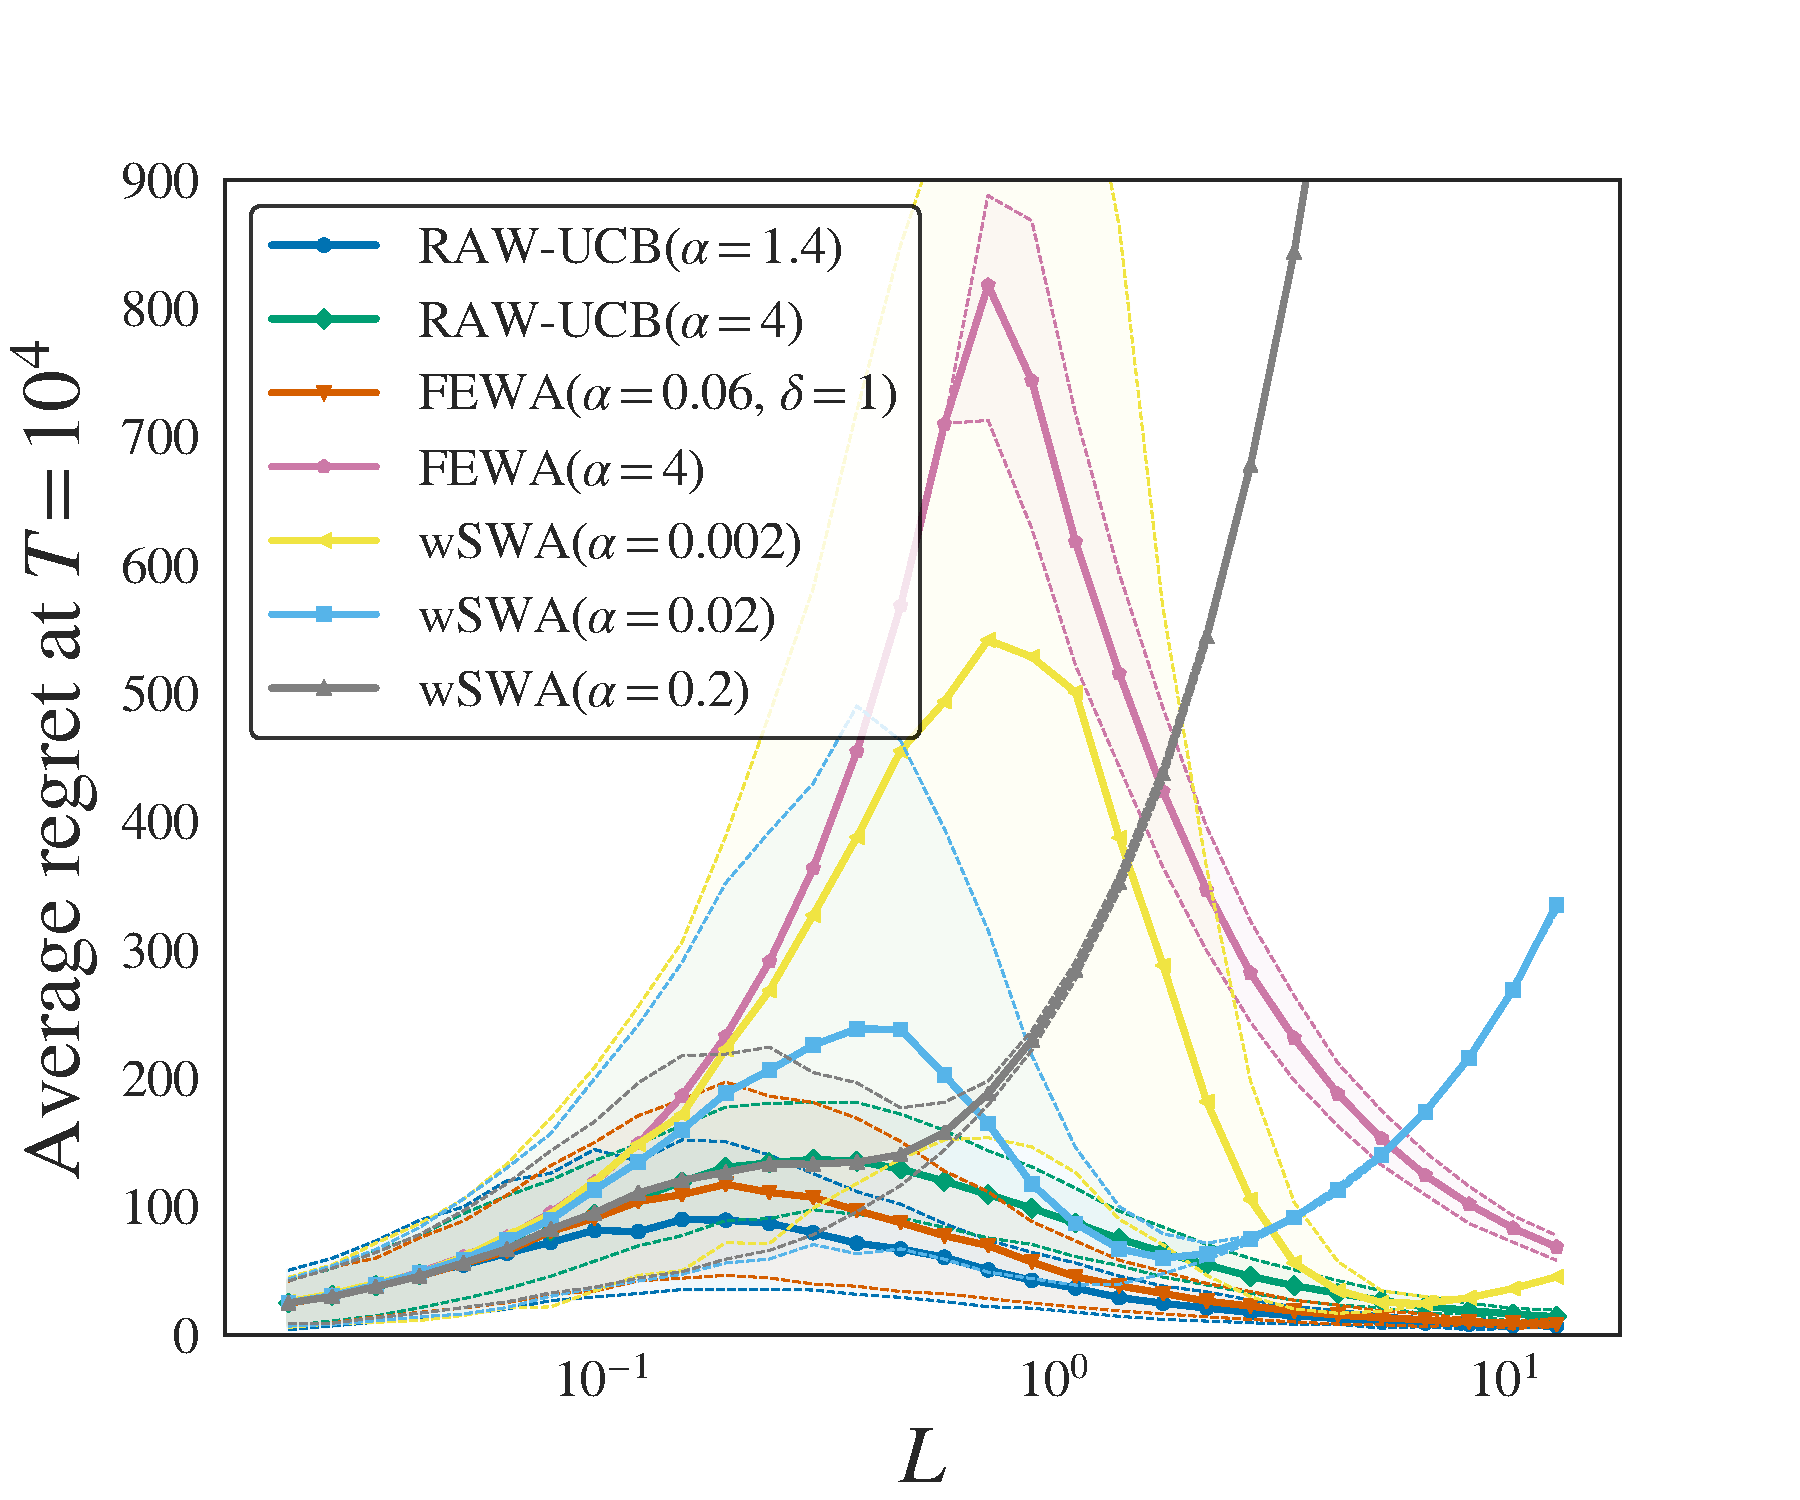
\includegraphics[clip, width= 0.51\textwidth]{2.1Rested/fig/fig1A_main.pdf}
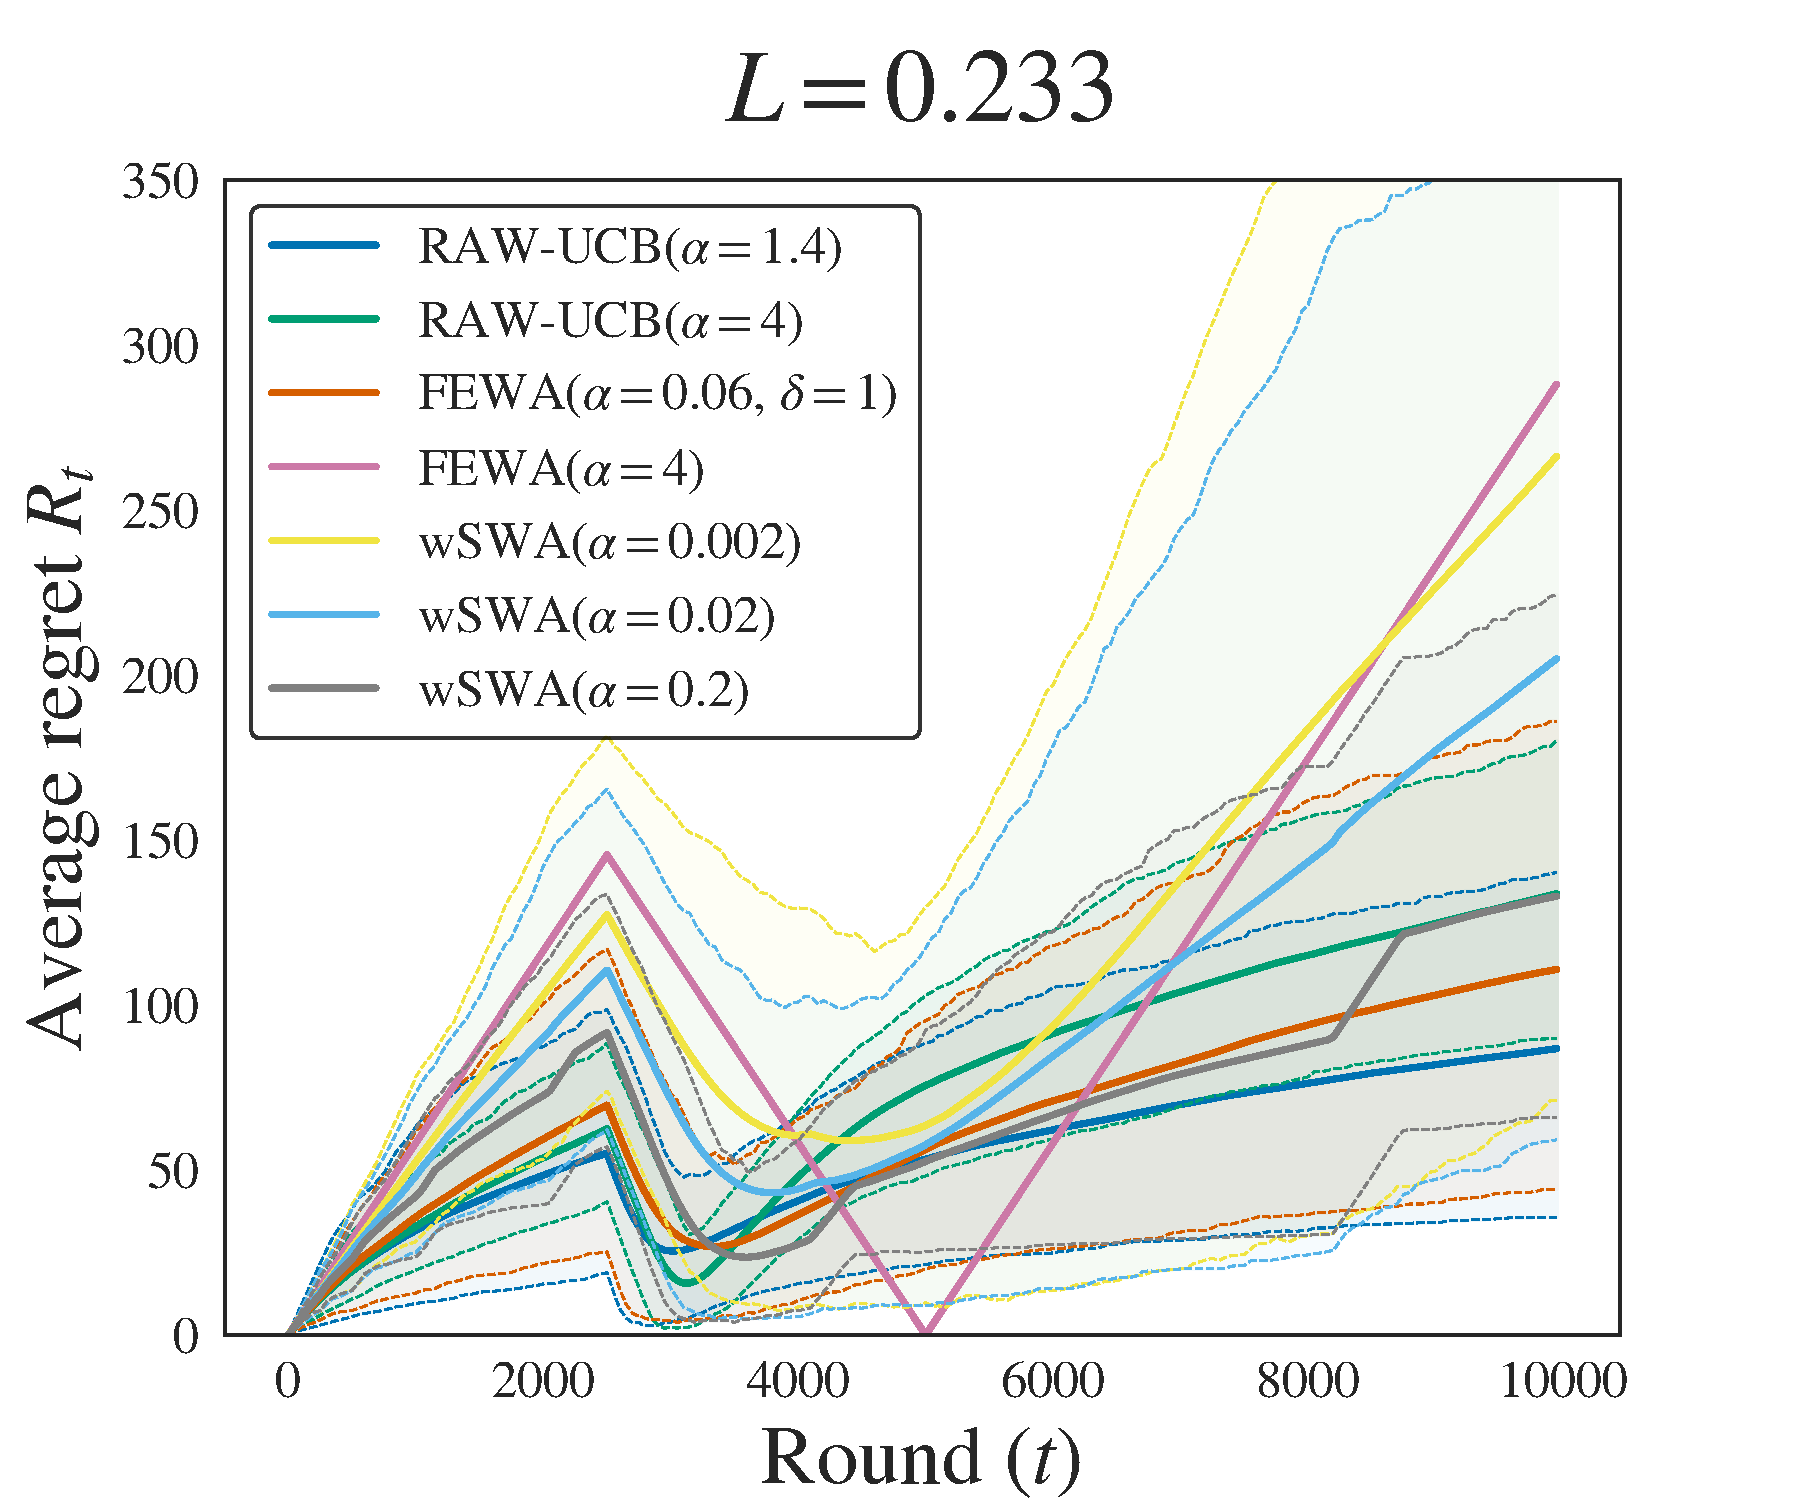
\includegraphics[clip, width= 0.49\textwidth]{2.1Rested/fig/fig1B_main.pdf}
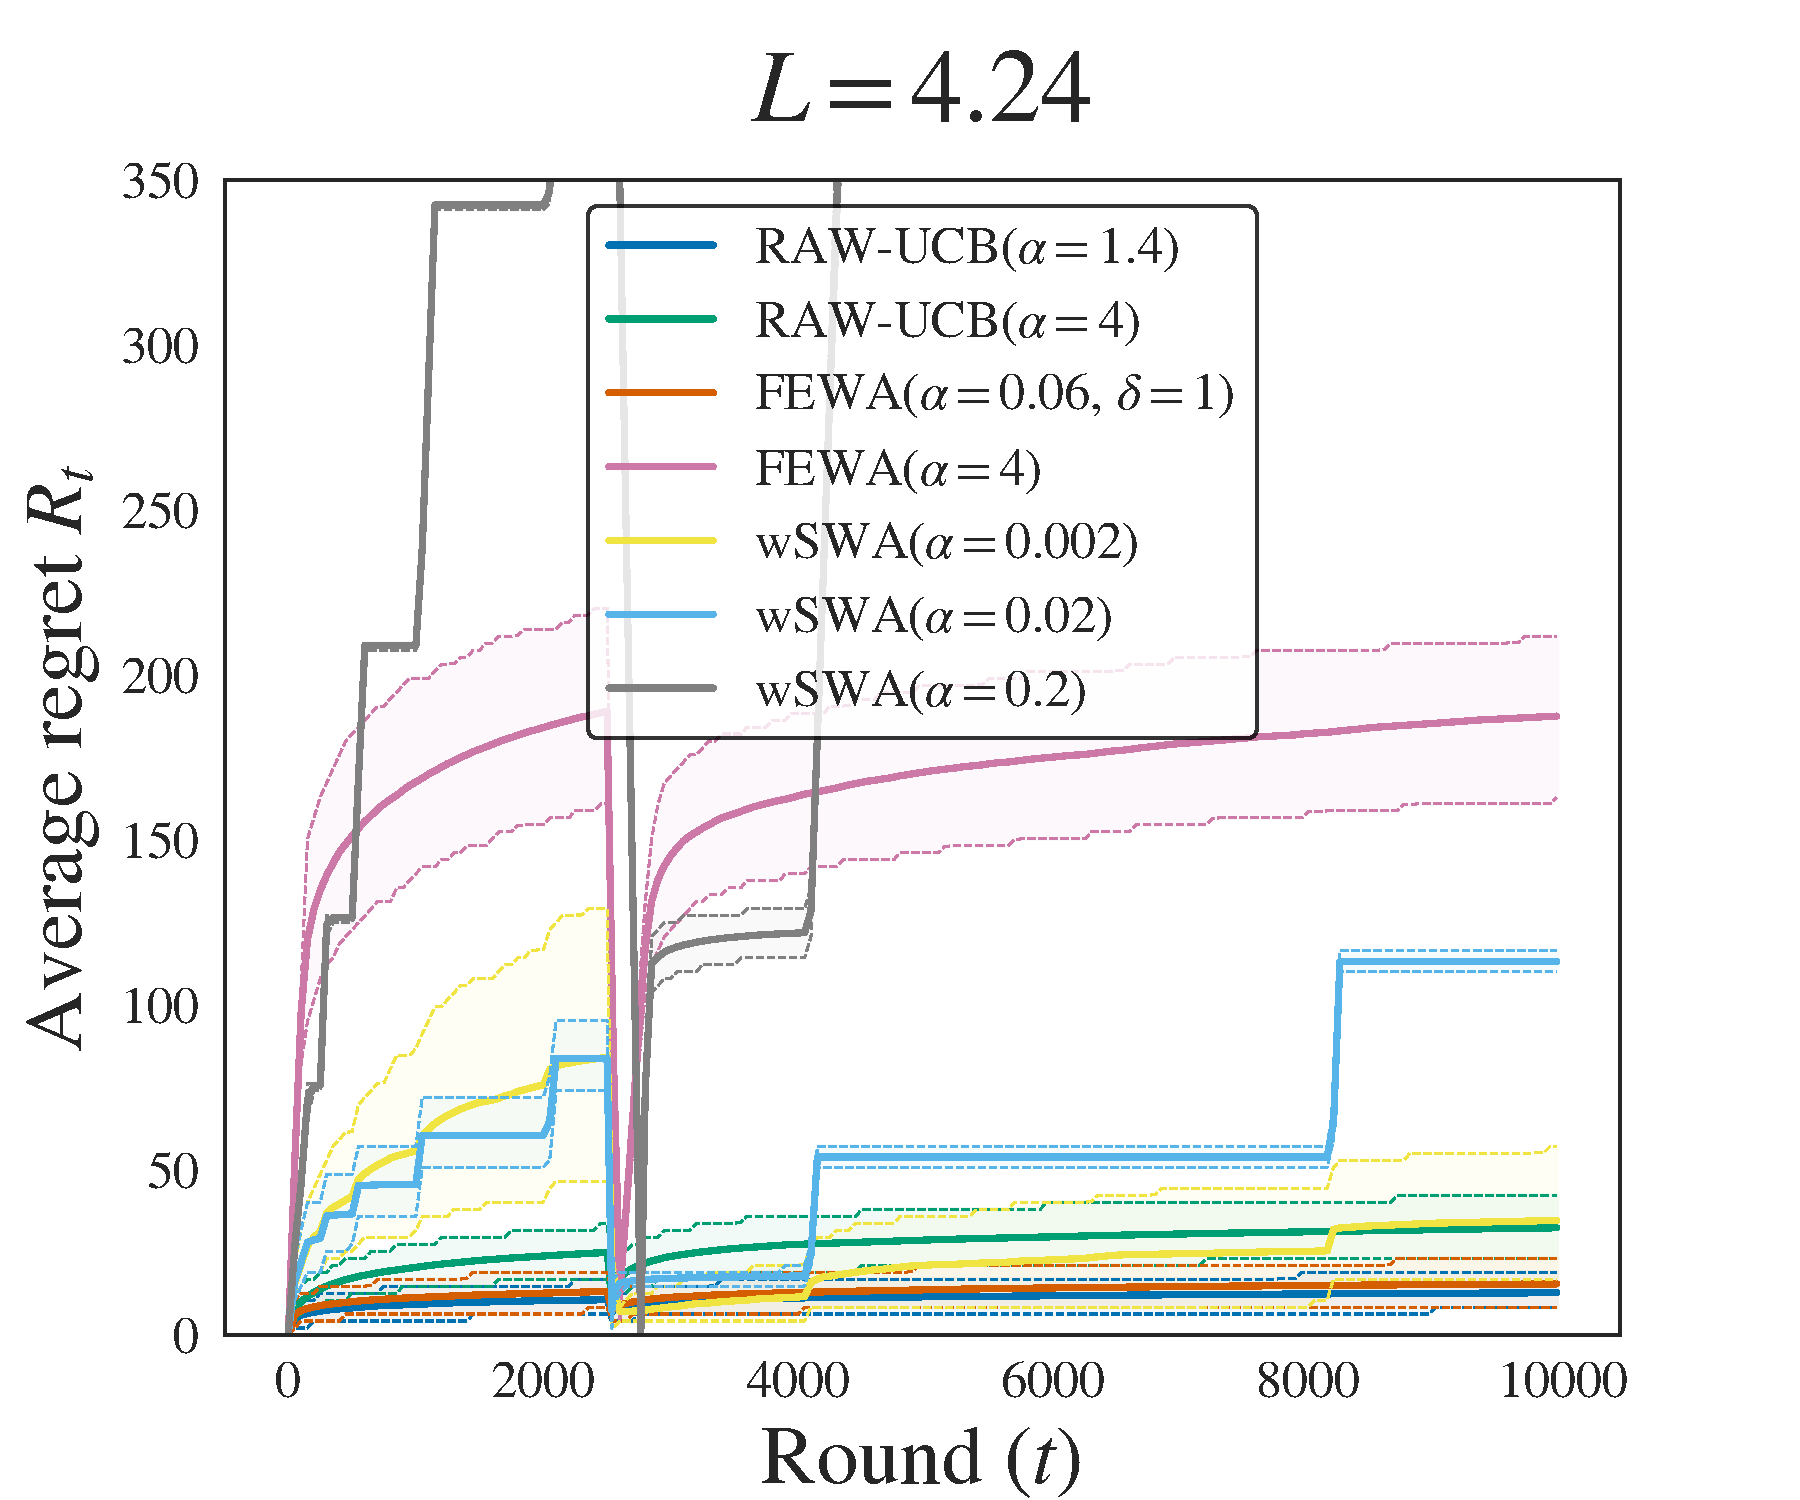
\includegraphics[clip, width= 0.49\textwidth]{2.1Rested/fig/fig1C_main.pdf}
\caption{\textbf{Top:} Regret at the end of the game for different values of $L$. \textbf{Bottom:} Regret across time for two values of $L$. Average over 1000 runs. We highlight the $\left[10\%, 90\%\right]$ confidence region.}
\label{fig:rested-exp1}
\end{figure*}

\paragraph{Algorithms.} We display the performance of \RAWUCB and \FEWA for two versions of each algorithm: with the theoretical tuning $\alpha = 4$; and with the empirical tuning $\alpha_{\mathrm{R}} = 1.4$ and $\alpha_{\mathrm{F}} = 0.06$. These two values are selected by grid-search. Though there are 30 different problems (for different $L$), the best tuning of $\alpha$ is the same for all the considered problem. We also include the three versions of \wSWA that we displayed in Subsection~\ref{subsec:rested-experiment1}.


\paragraph{Results - {\RAWUCB} versus {\FEWA}.} We compare \RAWUCB and \FEWA both for theoretical and empirical tuning. For theoretical tuning, we see in Figure~\ref{fig:rested-exp1} (top), that \RAWUCB outperforms \FEWA on all sizes of decays by a factor $\sim 4$ which is predicted by our theory. Indeed, there is also a factor 4 between the two problem-dependent upper-bounds (Theorem~\ref{th:rested-PD}). 

Surprisingly, for empirical tuning, the average performances of the two algorithms are much closer. We also notice that there is a larger variance in \FEWA's result compared to \RAWUCB. This is not surprising because we had to drastically reduce the confidence bounds to make \FEWA practical. It means that empirical \FEWA filters arms based only on a handful of samples. This bet leads to both very good and very bad runs. Last, Figure~\ref{fig:rested-exp1} (bottom) shows that \RAWUCB outperforms \FEWA at almost any time $t$, both on easy ($L=4.24$) and difficult ($L=0.233$) problems. The only round at which \FEWA shows better performance than \RAWUCB is after the regret decay. It is because \FEWA was less good at identifying the best arm in the first part of the game. Hence, just after the decay, it pulls more the other arm - which has become optimal. 

In the following, we will compare \RAWUCB with \wSWA. Notice that a similar comparison can hold for \FEWA ($\alpha=0.06$).

\paragraph{Results - Problem dependent performance and the impact of L.} \RAWUCB with the best empirical tuning improves over \wSWA on each problem (Figure~\ref{fig:rested-exp1} (top)). \RAWUCB with the theoretical tuning recovers quite good performance as well. 

In this setting, $L$ has two different meanings. It is the maximum decay per round (noted as $L$ in the theoretical section) and the gap between arms $\Delta_{2,h} = \nicefrac{L}{2}$ (for any $h$). According to our problem-dependent bound in Theorem~\ref{th:rested-PD}, the regret bound converges to $\cO\pa{KL}$ when $L$ and $\Delta_{2,h}$ are large with respect to $\sigma$. It tends to show that setup where arms are well separated from each other are easy problems for \FEWA and \RAWUCB. It is indeed confirmed in Figure~\ref{fig:rested-exp1} (top), where the regret of \FEWA and \RAWUCB converges to $\nicefrac{L}{2}$ when $L$ is large.

\paragraph{Results - Worst-case improvement.}
In Figure~\ref{fig:rested-exp1} (top), the worst regret for any of the two versions of \RAWUCB is smaller than the worst regret of any of the three versions \wSWA. Moreover, we remark that the regret at the round $T$ has one maximum for the variation of $L$ for \RAWUCB. This is not the case for \wSWA where the regret increases again for large values of $L$.

It confirms our analysis. Indeed, Theorem~\ref{th:rested-PI} shows a larger regret rate than Proposition~\ref{prop:SWA}. Moreover, the analysis shows that the worst cases for \RAWUCB correspond to cases where the learner does $\cO\pa{T}$ mistakes of intermediate size  $\cO\pa{\sqrt{\nicefrac{K}{T}}}$ which corresponds to the single maximum in Figure~\ref{fig:rested-exp1} (top).  

\paragraph{Results - Tuning and agnostic algorithms.}
Figure~\ref{fig:rested-exp1} (top) confirms that \FEWA and \RAWUCB do not rely on the knowledge of $L$. Indeed, the optimal tuning is the same for all the 30 problems. By contrast, the performance of \wSWA depends critically on the prior knowledge of  $L$: each of the three displayed tunings is the best for a specific range of $L$. 

Figure~\ref{fig:rested-exp1} (bottom) shows the advantage of anytime algorithms compared to the doubling trick. Indeed, the periodic restarts are quite expensive for \wSWA.  

\paragraph{Results - High-probability.}
We see that the variance of \wSWA is quite large for intermediate values of $L$. It confirms the analysis of \wSWA which shows two sources of the regret: the variance and the bias of the index. The regrets caused by variance has itself a large variance. Indeed, the sub-optimal arms are often correctly estimated, and hence not pulled by the index policy. It leads to many good runs of \wSWA. However, there are still many runs on which there is a sufficient deviation in the indexes which leads to very large regret. 

By contrast, the variance in the results is much more controlled by \RAWUCB and \FEWA. Indeed, when the statistics of these algorithms are not significant enough they tend to explore which leads to less large deviation of the regret. 

\subsection{Simulated benchmark $\#$2 (10 arms).}

\begin{figure*}[t]
\centering
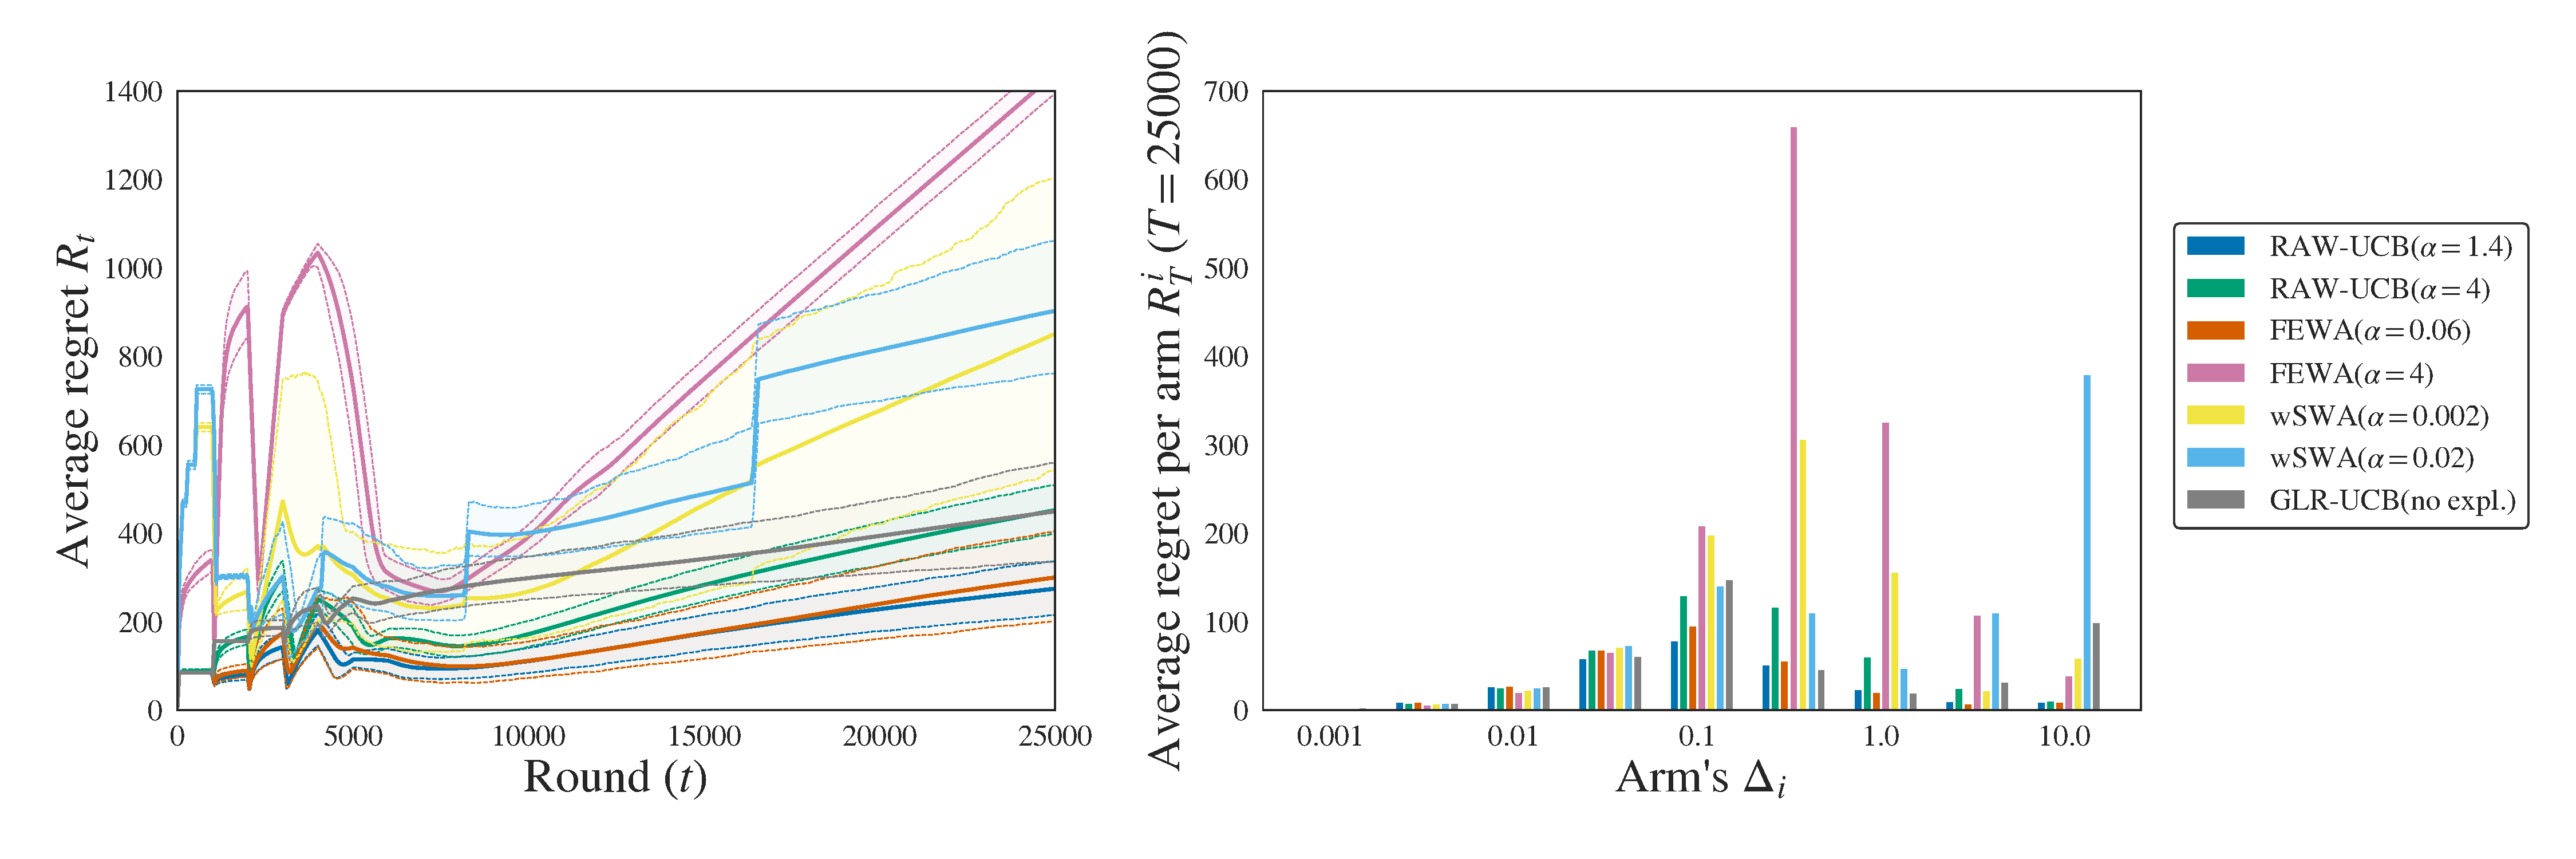
\includegraphics[width = 0.99 \textwidth]{2.1Rested/fig/fig2_main.pdf}
\caption{\textbf{Left:} Regret at the end of the game for different values of $L$. \textbf{Middle, Right:} Regret across time for two values of $L$. Average over 1000 runs. We highlight the $\left[10\%, 90\%\right]$ confidence region.}
\label{fig:rested-exp2}
\end{figure*}

\paragraph{Algorithms.} We display the same two versions of \FEWA and \RAWUCB. We also show the three best algorithms presented in Subsection~\ref{subsec:rested-experiment1}: two versions of \wSWA with $\alpha\in \left\{0.002, 0.02\right\}$ and \GLRUCB with no exploration. 

\paragraph{Results.}
The comparison between \RAWUCB, \FEWA, and \wSWA leads to a similar conclusion than for the two-arm bandit experiment. \RAWUCB and \FEWA show superior performance, except for the theoretical tuning of \FEWA which is too conservative. 

In particular, these algorithms show a better adaptation to each arm's gap. Indeed, the regret per arm is more controlled, especially for large values of the gaps, on which \wSWA suffers a large regret. There is also less deviation in the regret and we see the benefits of avoiding the doubling trick. 

In the two-arm setup with a single decay, it is possible to find a value of $\alpha$ for which \wSWA is correctly tuned for the specific decay. For instance, for $L\in \left[ 1, 3\right]$, \wSWA with $\alpha = 0.02 $ has almost the same performance than \RAWUCB (Fig.~\ref{fig:rested-exp1}). In the ten-arm setup with multiple decays, this is not possible anymore. Indeed, since there are several dropping values for each arm, there exists at least one arm on which the fixed window of \wSWA is not correctly tuned. For instance, for $\alpha = 0.002$ , \wSWA suffers a large regret on the arm with $\Delta_i = 0.3$. For \wSWA with $\alpha = 0.02$, the regret is large when $\Delta_i = 10$.

\RAWUCB and \FEWA also improve over \GLRUCB when their confidence bounds are tuned. We recall that \GLRUCB is an algorithm that uses a classical UCB index with a change detection procedure. When the change-detection procedure triggers, it erases the history of the changing arm. Notice that the confidence bounds of the index of \GLRUCB are already well-tuned, as they use the same confidence bounds as the asymptotic optimal tuning of \UCB. \GLRUCB shows sub-optimal performance on two arms $\Delta_i \in \left\{0.1, 10\right\}$. \GLRUCB suffers from the late restart for $\Delta_i = 0.1$.  Indeed, the change-point is hard to detect, and the index of the sub-optimal value is positively biased while it has not restarted. For $\Delta_i = 10$, the large regret of \GLRUCB is due to an implementation artefact. Indeed, we used the fast implementation for the change detector (by default in \citep{SMPyBandits}). It speeds up the algorithm but it can delay the change-detection scheme (by 10 pulls in this case). This delay leads to large regret when the mistake associated with each arm is large (as it is the case for $\Delta_i=10$).

\paragraph{Running time.}
\begin{table}[H]
\centering
\begin{tabular}{|c|c|}
\hline
\textbf{Policy} &\textbf{Running time (s)} \\ \hline
\FEWA($\alpha = 0.06$)    & 91                      \\ 
\FEWA($\alpha = 4$)      & 780                     \\ \hline
\RAWUCB ($\alpha = 1.4$) & 27                      \\
\RAWUCB($\alpha = 4$)    & 25                      \\ \hline
\wSWA($\alpha = 0.002$)   & 1                       \\ 
\wSWA($\alpha = 0.02$)    & 1                       \\ \hline
\GLRUCB          & 46 \\ \hline
\end{tabular}
  \caption{Average running time for the 10-arms experiment in seconds.}
  \label{tab:time-fig2}
\end{table}

In Table~\ref{tab:time-fig2}, we display the running time for this experiment. The computational experiments were conducted using the Grid’5000 experimental testbed \citep{grid5000}. For meaningful comparison, all the algorithms run on the same "Grenoble/dahu" cluster (2 CPUs Intel Xeon Gold 6130, 16 cores/CPU, 192GB RAM, 223GB SSD, 447GB SSD, 3726GB HDD, 1 x 10Gb Ethernet, 1 x 100Gb Omni-Path). 

\RAWUCB runs 25 times slower than \wSWA. We will provide a computational analysis in the next section but we can already relate this increased running time with the higher number of statistics \RAWUCB update and compare at each round.

The $\alpha$ parameter of \FEWA has a large impact on the running time. Indeed, the larger the $\alpha$, the less aggressive are the filters, the longer it takes to reach the end of the filtering process. Yet, even when $\alpha$ is small, \FEWA is slower than \RAWUCB. This is a consequence of the simplicity of the index policy over the filtering procedure. Indeed, in Python, we can use the fast C++ implementation of the scientific computing library Numpy to perform the most classical operations. Hence, for \RAWUCB, we only use the NumPy functions $\argmax$ and $\min$ to choose the next arm. For \FEWA, the comparison part is more custom: we had to implement the while-loop at Line~\ref{algline:fewa-while} with a Python loop, which is known to be quite slow. Notice that since the two algorithms use the same statistics we use the same function \UPDATE in both algorithms.

\GLRUCB is slower than \RAWUCB. Notice that it is already a fast version of \GLRUCB which runs the change-detection subroutine sparsely (approximately 10 to 100 times faster than the original \GLRUCB).
\begin{remark}
We emphasize the better characteristics of \RAWUCB over \FEWA: better bounds, better empirical performances, easier and faster implementation, a better agreement between theory and practice, closer to the classical \UCB. For these reasons, we will focus our future empirical investigation on \RAWUCB.
\end{remark}
%!TEX root = ../main.tex 
\section{Efficient algorithms}
\label{sec:fast}
\subsection{The numerical cost of adaptive windows}

In the three last sections, we presented two adaptive windows algorithms that significantly improved over state-of-the-art algorithms, both theoretically and experimentally. Yet, our numerical experiments indicate that these improvements are computationally expensive. Indeed, at each round $t$, we store, update and compare $\cO\pa{t}$ statistics. 

The full update of the statistics can be done at a worst case cost of $\cO\pa{t}$. Indeed, each statistics $\hmu_i^h$ can be refreshed with a $\cO\pa{1}$ operation: 
\[\hmu_i^{h+1}(n+1) = \frac{h}{h+1}\hmu_i^{h}(n) + \frac{1}{h+1}o_t \,. \]

The comparison part in both \FEWA and \RUCB is also a $\cO\pa{t}$ operations. In \FEWA , we do a scan based on $\hmu_i^{h}$ for all $i \in \arms_h$ with increasing $h$. Hence, the total number of unitary operations is in $\cO\pa{t}$ in the worst case, as it scales with the number of statistics. \RUCB computes one UCB for each of the $\cO\pa{t}$ statistics. For each arm, it selects the minimum UCB as the index, which can be done with complexity $\cO\pa{t}$. Finally, finding the largest index is a $\cO\pa{K}$ operation. Therefore, we can conclude,

\begin{proposition}
At any round $t$, \FEWA and \RUCB have a $\cO\pa{t}$ worst-case complexity in time and memory.
\end{proposition}

\begin{remark}
\SWA($h$) has a $\cO\pa{h}$ worst-case complexity in time and memory because the sliding-window mechanism needs to store and update $\cO\pa{h}$ statistics to always have the average of the $h$ last sample ready. Hence, when it is optimally tuned for the minimax bound, $\SWA$ has a $\cO\pa{T^{2/3}}$ per round complexity. As often in non-stationary bandits, it may be possible to replace sliding window statistics with discounted statistics. Such modification often leads to a slightly worse theoretical regret rate with a much better $\cO\pa{K}$ complexity. 
\end{remark}

Hence, handling a large number of windows, which is the main strength of our algorithms to achieve a lower regret, is a significant drawback when it comes to design fast algorithms. Therefore, it is an open question whether one can enjoy the benefits of adaptive windows without suffering large time and space complexity. 

\subsection{The efficient update trick}
We detail \EFF, an update scheme to handle efficiently statistics of different windows. A similar yet different approach has appeared independently in the context of streaming mining~\citep{bifet2007learning}. \EFF is built on two main ideas: \emph{geometrically sparse} and \emph{delayed} statistics.

First, at any time $t$ we can avoid using $\left\{\hmu_i^h\right\}_{h}$ for all possible windows $h$ starting from 1 with an increment of 1. In fact, both statistics $\hmu_i^h$ and constructed confidence levels $c(h, \delta_t)$  have very close value for successive $h$ as $h$ becomes large: 
\begin{align*}
& \hmu_i^{h+1}(n) = \hmu_i^{h}(n) + \cO\pa{\frac{\sigma + L}{h}}\,,\\
& c(h+1, \delta_t) = c(h, \delta_t) + \cO\pa{\frac{\sigma }{h^{3/2}}} \,.
\end{align*}
Hence, in both \FEWA and \RUCB, we compute a lot of very similar quantities. Instead, we could use fewer statistics which are significantly different: $\left\{\hmu_i^h(\Nitmonepi)\right\}_{h\in \Him}$, where the window $h$ is dispatched on a geometric grid, 
 \[\Him\pa{\Nitmonepi} \triangleq \left\{ h_j \in  \left\{1, \dots , \Nitmonepi \right\} \;|\; h_{j+1} = \ceil{m \cdot h_j} \text{ and } h_1 = 1\right\}\quad \text{with } m > 1.\]

When there is no confusion, we drop the dependency on $\Nitmonepi$.  This modification alone is not enough to reduce both the time and space complexity. Indeed, updating $\hmu^h_{i}$ requires to replace the $h$-th last sample by the new one $o_t$. Hence, we need to store the $t$ collected samples to be able to update any $\hmu^h_{i}$  with $\cO\pa{1}$ complexity. Therefore, in \EFF, we will use $\cO\pa{K\log\pa{t}}$ \emph{delayed} statistics that we can update with $\cO\pa{K\log\pa{t}}$ space and time complexity.

\EFF (Alg.~\ref{alg:effupdate}) takes as input the new observation $o_t$ that the learner gets at the $N_i$-th pull of arm $i$; the geometric window grid $\Him$ tuned with an hyperparameter $m>1$, and for each window $h_j$ in this grid, three different numbers $\hmueff,\; \peff, \; \neff$. $\left\{\hmueff\right\}_{i,h_j}$ represents the set of \emph{current} statistics of window size $h_j$ that will be used instead of $\left\{\hmu_i^h\right\}_{i,h}$ in our efficient algorithms. We also store a pending statistic $\peff$ and a count $\neff$  which are used in the sparse update procedure of $\hmueff$. \EFF outputs an updated set of statistics.  
\begin{figure*}[!ht]
\begin{minipage}{\textwidth}
\renewcommand*\footnoterule{}
\begin{savenotes}
\begin{algorithm}[H]
\caption{{\EFF}}
\label{alg:effupdate}
\begin{algorithmic}[1]
\Require $o_t$, \small $\Him \gets \left\{h_j \! <\! \ceil{m \cdot N_i} \; | \;  h_{j+1} \!=\! \ceil{m \cdot h_j}  \text{with } h_0 \!=\! 1\right\} $\normalsize, $\left\{ \{ \hmueff,\, \peff, \, \neff \}\right\}_{h_j \in \Him}$
\If{$N_i = \max\pa{\Him}$}\label{algline:effu-new-condition} \Comment{Create a new triplet with window $h_j = \ceil{m \cdot N_i}$}  
\State $\Him \gets \Him \cup \left\{ \ceil{m \cdot N_i} \right\}$\label{algline:effu-new-h}
\State $p_i^{\ceil{m \cdot N_i} } = p_i^{N_i} $\label{algline:effu-new-p}
\State $n_i^{\ceil{m \cdot N_i} } \gets n_i^{N_i} $\label{algline:effu-new-n}
\State $\hmu_{i, \, \tteff}^{\ceil{m \cdot N_i} }\leftarrow \texttt{None}$\label{algline:effu-new-mu}
\EndIf\label{algline:effu-new-end} 
\State $p_i^{1} \gets o_t$ \label{algline:effu-update-first-p} \Comment{Update the first triplet with $o_t$}
\State $n_i^{1} \gets 1$\label{algline:effu-update-first-n}
\State $\hmu_{i, \, \tteff}^{1}\leftarrow o_t$ \label{algline:effu-update-first-hmu}
\For{$h_j \in  \Him \smallsetminus \left\{ 1\right\} $}\label{algline:effu-update-start} \Comment{Update the other pending statistics $\peff$ and $\neff$}
\State $p_i^{h_j} \gets p_i^{h_j}  +o_t$\label{algline:effu-update-p}
\State $n_i^{h_j} \gets n_i^{h_j} + 1$\label{algline:effu-update-n}
\EndFor\label{algline:effu-update-end} 
\For{$h_j \in  $ \textsc{Sort\_Desc}$\pa{\Him \smallsetminus \left\{ 1\right\} }$}\label{algline:effu-refresh-start}
\If{$n_i^{h_j} = h_j$} \label{algline:effu-refresh-condition}
\State $\hmueff \leftarrow p_i^{h_j}/h_j$ \Comment{Replace the current statistic $\hmueff$}\label{algline:effu-refresh-hmu}
\State{$p_i^{h_{j}} = p_i^{h_{j-1}} $} \label{algline:effu-refresh-p}\Comment{Refresh the pending statistics}
\State $n_i^{h_{j}} \gets n_i^{h_{j-1}} $\label{algline:effu-refresh-n}
\EndIf
\EndFor \label{algline:effu-refresh-end}
\Ensure $\left\{\left\{  \hmueff,\; p_i^{h_j}, \; n_i^{h_j} \right\}\right\}_{h_j \in \Him}$
\end{algorithmic}
\end{algorithm}
\end{savenotes}
\end{minipage}
\end{figure*}
The core of \EFF is divided in four parts: 1) From Lines~\ref{algline:effu-new-condition} to~\ref{algline:effu-new-end}, we create new window's statistics at a logarithmic rate with respect to the growth of $N_i$; 2) From Lines~\ref{algline:effu-update-first-p} to~\ref{algline:effu-update-first-hmu}, we update the statistics of window $h_1=1$;
3) From Lines~\ref{algline:effu-update-start} to~\ref{algline:effu-update-end}, we update the other pending statistics and count;
4) From Lines~\ref{algline:effu-refresh-start} to~\ref{algline:effu-refresh-end}, we eventually update $\hmueff$ and refresh the corresponding pending statistic and count. The remaining details are quite technical. Thus, we first give the high-level properties that are ensured by the recursive usage of \EFF. Then, we prove them by going through the algorithm line by line.\newpage

\begin{proposition}
\label{prop:effu}
 $\left\{\left\{  \hmueff,\; p_i^{h_j}, \; n_i^{h_j} \right\}\right\}_{h_j \in \Him}$, constructed recursively with \EFF with initial value $\left\{\left\{  \hmu_{i,\,\tteff}^1 : \texttt{None},\; p_i^{1} :0 , \; n_i^{1}:0 \right\}\right\}$ have the following properties:
 \begin{enumerate}[topsep=0pt]
  \item $\hmueff$ is the average of exactly $h_j$ consecutive samples among the $2h_j -1$ last ones. \label{list:effu-hmu}
  \item The delay between two updates of $\hmueff$ is in $\left\{\ceil{\frac{m-1}{m} h_j}, \dots, h_j -1\right\}$.\label{list:effu-delay}
%  \item When $m = 2$, $h_j = 2^{j}$. Moreover, for $j\geq1$,  the $k$-th update $\hmueff$ happens at pull $ \pa{k+1} \cdot 2^{j-1}$, \ie every $2^{j-1}$ pulls (and at every rounds for $j=0$).\label{list:effu-m2}
  \item $\peff$ is the sum of the $\neff$ last samples. \label{list:effu-p}
  \item $\neff < h_j$ for $j\geq 1$. Also, $n_i^1 \leq 1$.\label{list:effu-n1}
  \item $\left\{ \neff \right\}_{h_j}$ is an non-decreasing sequence with respect to $h_j$ (or $j$).\label{list:effu-n2}
 \end{enumerate}
\end{proposition}
\begin{proof}
The three last properties are trivially true at the initialization. Thus, we show by induction that they remain true after updates.
\paragraph{Proof of \ref{list:effu-p}. } At Lines~\ref{algline:effu-new-p} and~\ref{algline:effu-new-n}, we create a new pending statistics and count by initializing them with other statistics and counts. Hence, because of the recursion hypothesis, all the pending statistics $\peff$ (including the created one) contains the sum of the $\neff$ \emph{before last} pulls. At Lines~\ref{algline:effu-update-first-p} and~\ref{algline:effu-update-first-n}, we update $p_i^1$ with the last sample and set $n_i^1$ to $1$. At Lines~\ref{algline:effu-update-p} and~\ref{algline:effu-update-n}, we add the last sample to $\peff$ (which was containing the before last samples) and increase the count by $1$. Hence, at the end of Line~\ref{algline:effu-update-n}, all the $\peff$ contains the sum of the last $\neff$ samples. Thus, refreshing $\peff$ and $\neff$ with $ p_i^{h_{j-1}}$ and $n_i^{h_{j-1}}$ keeps this property true (Lines~\ref{algline:effu-refresh-p} and~\ref{algline:effu-refresh-n}). 

\paragraph{Proof of \ref{list:effu-n1}.}
For $j=0$, $n_i^1$, which is equal to $0$ at the initialization, is set at $1$ at every update (Line~\ref{algline:effu-update-first-n}). Hence, we have $n_i^{h_0} \leq h_0=1$.
For $j\geq 1$, $n_i^{\ceil{m \cdot N_i}}$ is initialized at Line~\ref{algline:effu-new-n} with the value $n_i^{N_i} < N_i < \ceil{m \cdot N_i}$ by the induction hypothesis and because $m>1$.  Then, $\neff < h_j$ ($j\geq1$) is increased by one at each update at Line~\ref{algline:effu-update-n}. Hence, we now have $\neff \leq  h_j$ for all $j\in\Him$. However, for $j\geq 1$, if $\neff = h_j$ (Line~\ref{algline:effu-refresh-condition}), it is replaced by the precedent count $n_i^{h_{j-1}}\leq h_{j-1} < h_j$ (Line~\ref{algline:effu-update-n}). Thus, at the end of the update, we do have $\neff < h_j$ for $j\geq1$.

\paragraph{Proof of \ref{list:effu-n2}.}
At Line~\ref{algline:effu-new-n}, we create a new pending count corresponding to the largest $h_j$ and we initialize it with the precedent largest count. At Lines~\ref{algline:effu-update-first-n} and~\ref{algline:effu-update-n}, we set $n_i^1 =1$ and increase all the other $\neff$ by one. This operation preserves the non-decreasing property of the ordered set. Last, at Line~\ref{algline:effu-refresh-n}, we set few counts $\neff$ to the precedent value $n_i^{h_{j-1}}$- which also preserves the non-decreasing property of the ordered set. 

\paragraph{Proof of \ref{list:effu-hmu} and \ref{list:effu-delay}.}
Thanks to Property~\ref{list:effu-p}, we know that $\peff$ is the sum of the $\neff$ last sample. It is still true at the end of Line~\ref{algline:effu-update-n} (see the proof). Then, at Line~\ref{algline:effu-refresh-hmu}, and given the condition in Line~\ref{algline:effu-refresh-condition}, we set $\hmueff$ with the average of the last $h_j$ sample. Then, $\hmueff$ is not updated untill the condition at Line~\ref{algline:effu-refresh-condition} is fulfilled again. 

$\neff$ is refreshed with a quantity larger or equal to $1$ and smaller or equal to $h_{j-1}$ at Line~\ref{algline:effu-refresh-n}. Then, it is increased by one at each update. we know that $\hmueff$ will be updated at least every $h_j-1$, and at most every $h_j -h_{j-1}$ round. Hence, considering the worst possible delay we can conclude: $\hmueff$ is the average of exactly $h_j$ consecutive samples among the $2h_j -1$ last ones. Last, considering that $h_{j-1}\leq h_j /m$, we conclude that the minimal delay is larger or equal to $\frac{m-1}{m}h_j$.
\end{proof}

In Proposition~\ref{prop:effu-complexity}, we show that \EFFU succeeds to drastically reduce the time and space complexity of the updates as soon as $m$ is not too close to $1$.
\begin{proposition}
\label{prop:effu-complexity}
After $N_i$ updates, the time and space complexity of \EFFU scales with $\cO\pa{\min\pa{ \log_m{N_i}, N_i}} $.
\end{proposition}
\begin{proof}
The time and space complexity scales with $|\Him|$. Indeed, there are $3|\Him| + 2$ variables store in memory : $\left\{ \{ \hmueff,\, \peff, \, \neff \}\right\}_{h_j \in \Him}$, $o_t$ and $N_i$. Moreover, \EFFU does two $\textsc{For}$ loops on $\Him$.

The size of $\Him$ is upper-bounded by $\cO\pa{\log_m N_i}$. Indeed, when the condition at Line~\ref{algline:effu-new-condition} is fulfilled, $\max\pa{\Him}$ is replaced by $\ceil{m\cdot N_i}$. When it is not fulfilled, the maximum is not changed but $N_i$ increases by one unit. Hence, we always have, 
\[
\max\pa{\Him} \leq \ceil{m\cdot N_i}.
\]
Moreover, when the condition is fulfilled, the maximum is replaced by,
\[
\max\pa{\Him} \leftarrow \ceil{m \cdot\max\pa{\Him}}.
\]
Hence, when $\Him$ is initialized with $\left\{1\right\}$, we show recursively that, 
\[\max\pa{\Him} \geq m^{|\Him|-1}. \]
Combining the above equations, we have, 
\[m^{|\Him|-1} \leq m\cdot N_i +1. \]
Therefore, 
\[|\Him| \leq \log_m\pa{2N_i} + 2. \]
This upper-bound diverges at finite $N_i$ when $m\rightarrow 1$. However, the size of $\Him$ is increased one by one at Line~\ref{algline:effu-new-h}. Hence, even if the condition at Line~\ref{algline:effu-new-condition} is fulfilled at every round, $|\Him|\leq N_i +1$ ($\Him$ is initialized with $\left\{1\right\}$).
\end{proof}

\begin{remark}
When $m\leq 1 + \frac{1}{N_i}$, $\left\{\hmueff\right\}_{h_j \in \Him}$ (the outcome of \EFFU) is the same than the outcome of the classical update $\left\{\hmu_i^h\right\}_{h \leq N_i}$ for the $N_i$ first rounds. Yet, there is no free lunch, the complexity is $\cO\pa{N_i}$ in this regime (according to Proposition~\ref{prop:effu-complexity}).
\end{remark}



\subsection{The delay in {\EFF}}
We have already emphasized that \EFFU is built on two ideas: geometrically sparse and delayed statistics. The geometrically sparse aspect is straightforward to understand and quantify: $h_{j+1} \sim m \cdot h_j$ up to the rounding.

In this Subsection, we provide a tight analysis of the delay between the updates. In fact, the important quantity is the normalized delay, that is, the delay divided by the window size. Indeed, each statistic of window $h_j$ should represent the $h_j$ last sample. A delay of $10$ for $h_j = 10^6$ is very good as it succeeds to take into account most of the $h_j$ last sample. However, the same delay of $10$ is a failure when $h_j = 1$, as the algorithm fails to give a good representation of the very last sample.

In Property~\ref{list:effu-delay}, we show that the normalized delay cannot be larger than $100\%$. We also show that it is lower bounded by $\frac{m-1}{m}$. For small values of $m$, this amplitude can be large. 

We use two tricks in the algorithm to reduce the delay. First, at Line~\ref{algline:effu-refresh-n}, we refresh $\peff$ with $p_i^{h_{j-1}}$ which contains $n_i^{h_{j-1}} \in \left\{ 1, \dots, h_{j-1}\right\}$ samples. We could refresh $\peff$ and $\neff$ at $0$ which would lead to $100\%$ normalized delay. Instead, we use the variable available in the memory which contains the sum of $h$ last sample, with the largest $h< h_j$.  According to Properties~\ref{list:effu-p},~\ref{list:effu-n1} and~\ref{list:effu-n2}, this quantity is $p_i^{h_{j-1}}$. 

Indeed, according to Property~\ref{list:effu-p}, $p_i^{h_{j'}}$ contains the $n_i^{h_{j'}}$ last samples. At the round of the update of $\hmueff$,  $p_i^{h_{j'}}$ contains $h_j$ samples before Line~\ref{algline:effu-refresh-p}. According to Property~\ref{list:effu-n2}, all the $j'>j$ have  $n_i^{h_{j'}}>\neff = h_j$. According to Property~\ref{list:effu-n1}, $n_i^{h_{j-1}}\leq h_{j-1} < h_j$.  Moreover, for all $j' \leq j-1$, $n_i^{h_{j-1}} \geq n_i^{h_{j'}}$ (Property~\ref{list:effu-n2}).

The second trick is to sort $\Him$ in the decreasing order at Line~\ref{algline:effu-refresh-start}. If there are two synchronous consecutive updates of $\hmueff$ and $\hmu_{i,\, \tteff}^{h_{j+1}}$ at the same run of \EFF, doing a backward loop guarantees to refresh $n_i^{h_{j+1}}$ with $\neff = h_j$ instead of a smaller value if we would do a forward loop.

In this Subsection, we show that these two tricks succeed to upper-bound the normalized delay by $\cO\pa{\frac{m-1}{m}}$ when $m$ is an integer and when $m < 2$.


\subsubsection{The integer case.}
\begin{proposition}
\label{prop:effu-delay-int}
When $m \in \NN \setminus \left\{ 0, 1\right\}$,  $h_j = m^j$. Moreover, $\hmueff$ is updated periodically with period $\omega_j = \frac{m-1}{m} h_j$ for $j\geq1$ ($\omega_0 =1$).
\end{proposition}


The main idea is simple: since any window $h_j$ is a multiple of the lower order $h_{j-k}$, $\hmueff$ is initialized and updated synchronously with all the lower order statistics. Hence, the pending statistic $\peff$ is refreshed with $h_{j-1}$ sample, the largest possible number of sample in $p_i^{h_{j-1}}$. Hence, choosing integer values minimizes the delay (compared to the delay bounds we identify in Property~\ref{list:effu-delay}). The proof is quite technical, and we delay it at the end of the Subsection. 

\begin{figure*}[ht]
\centering
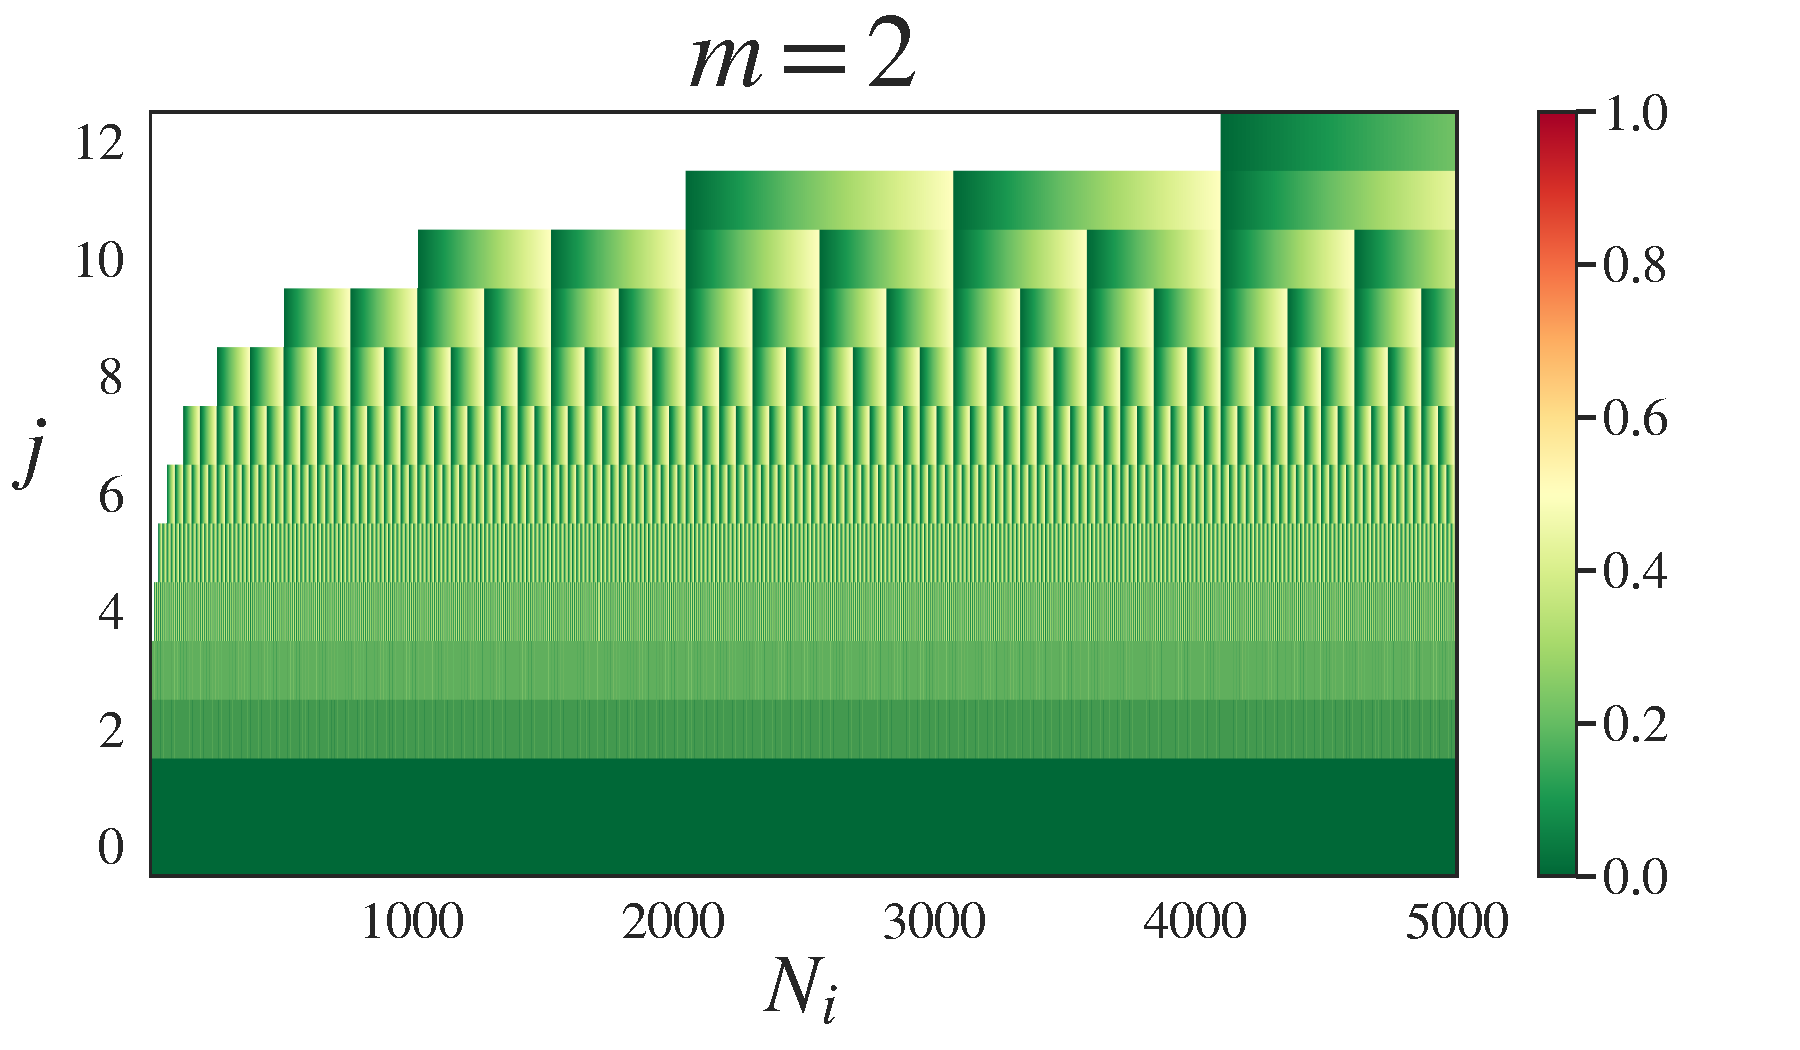
\includegraphics[clip, width= 0.49\textwidth]{2.1Rested/fig/T=5000_m=2.pdf}
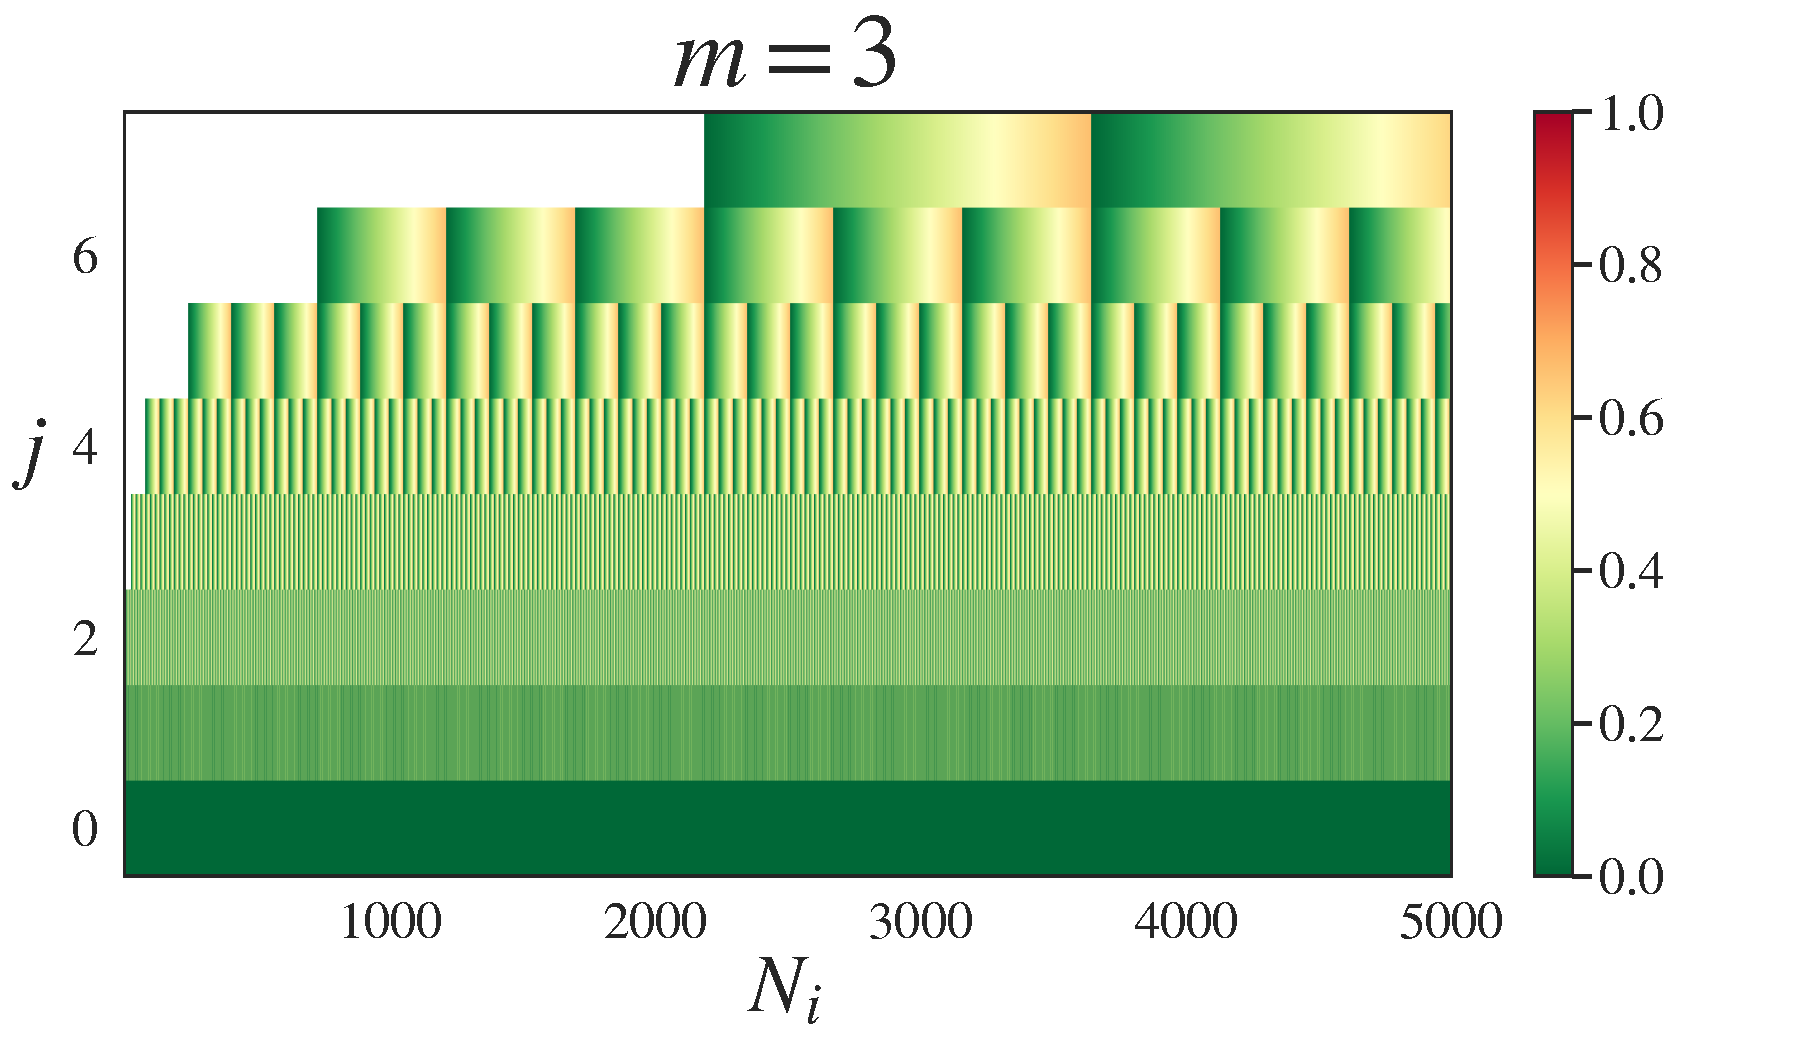
\includegraphics[clip, width= 0.49\textwidth]{2.1Rested/fig/T=5000_m=3.pdf}
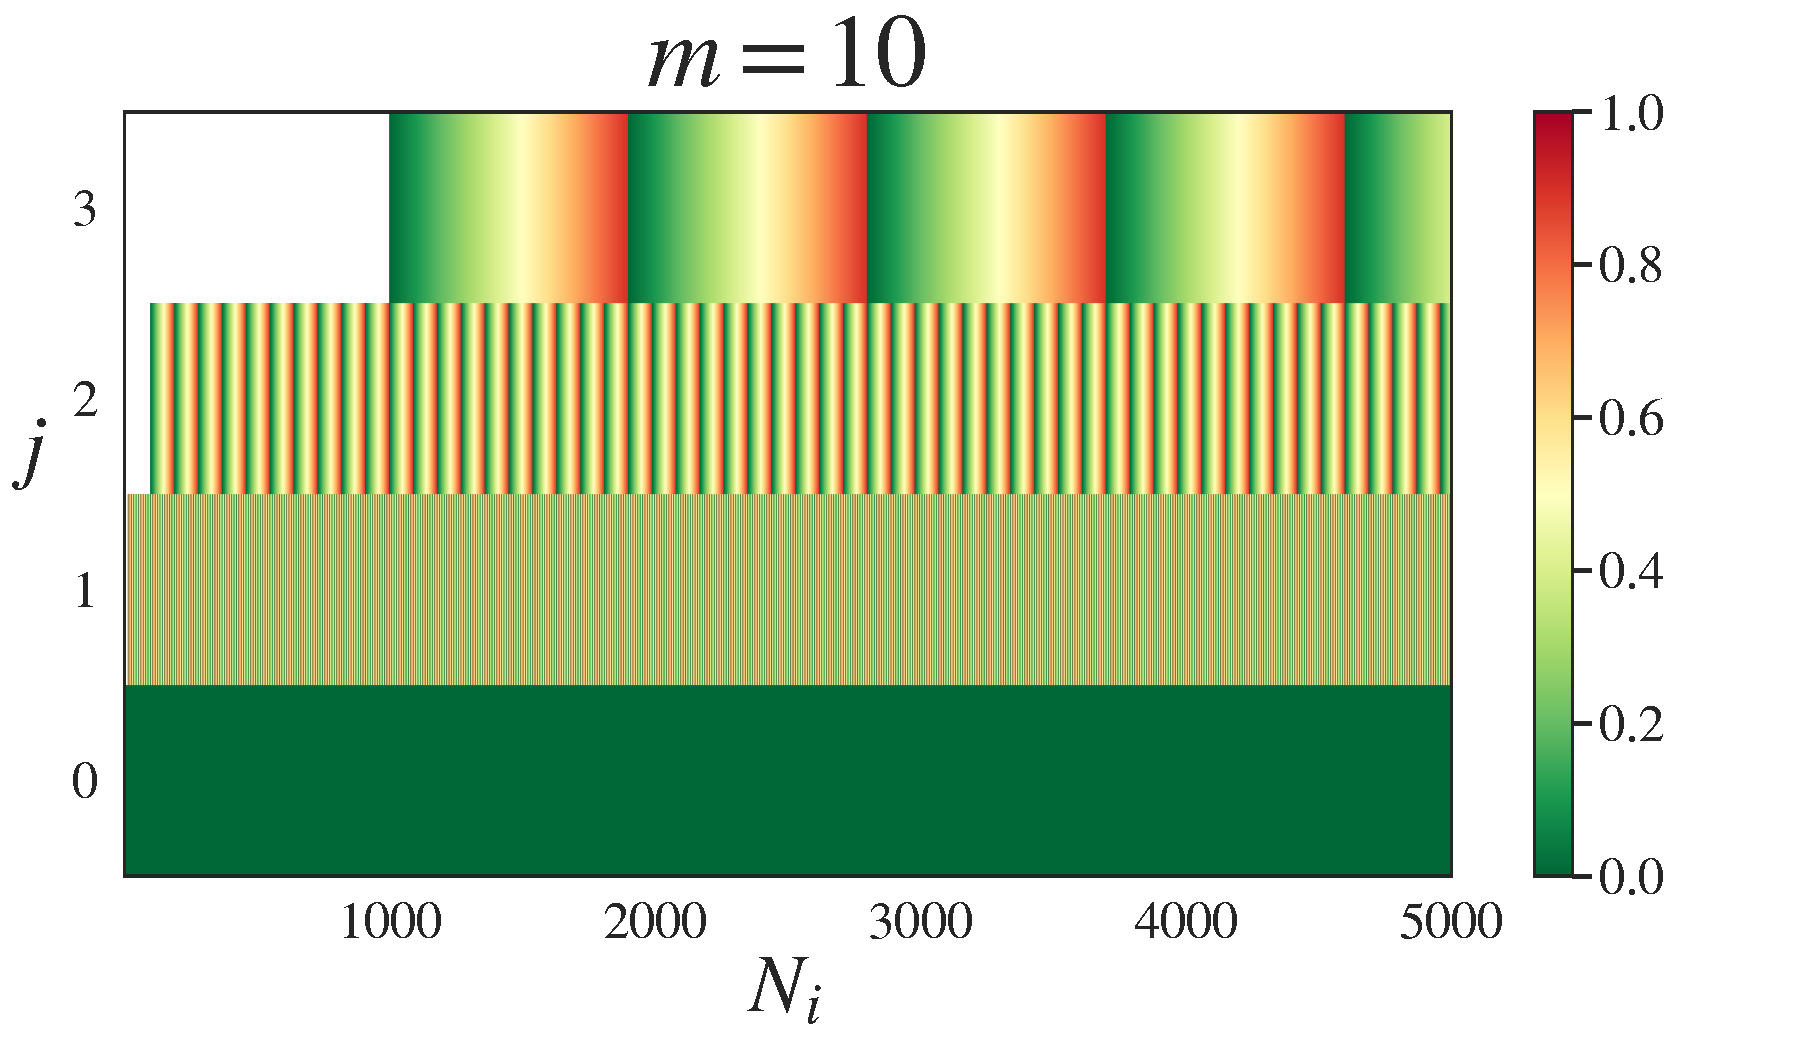
\includegraphics[clip, width= 0.49\textwidth]{2.1Rested/fig/T=5000_m=10.pdf}
\caption{Normalized delay $\nicefrac{d_j}{h_j}$ after $N_i$ pulls for each$j$-th statistic $\hmueff$. We display in white the rounds at which statistic $j$ is not created yet.}
\label{fig:delay-int}
\end{figure*}

We call $d_j(N_i) \in \left\{0, \dots, \omega_j-1 \right\}$, the number of pulls since the last update of statistic $\hmueff$ after $N_i$ pulls. We display in Figure~\ref{fig:delay-int}  
the normalized delay $\nicefrac{d_j}{h_j}$ after $N_i$ pulls of each statistic. The updates are indeed periodic. We notice the strong synchronization in the updates: not only each period $\omega_j$ is at a $m$ factor of the previous one, but the update of statistic $j$ are at the same round as the updates of statistics $j'<j$. %Figure.

However, for large values of $m$, the delay improvement is marginal. For $m=10$, each statistic can be delayed by $90\%$ their window size. Even, for $m=2$ the normalized delay $\nicefrac{\omega_j}{h_j}$ is $50\%$. The $\nicefrac{m-1}{m}$ ratio would be very interesting for $m \rightarrow 1$. 

\subsubsection{The non integer case}
\begin{figure*}[ht]
\centering
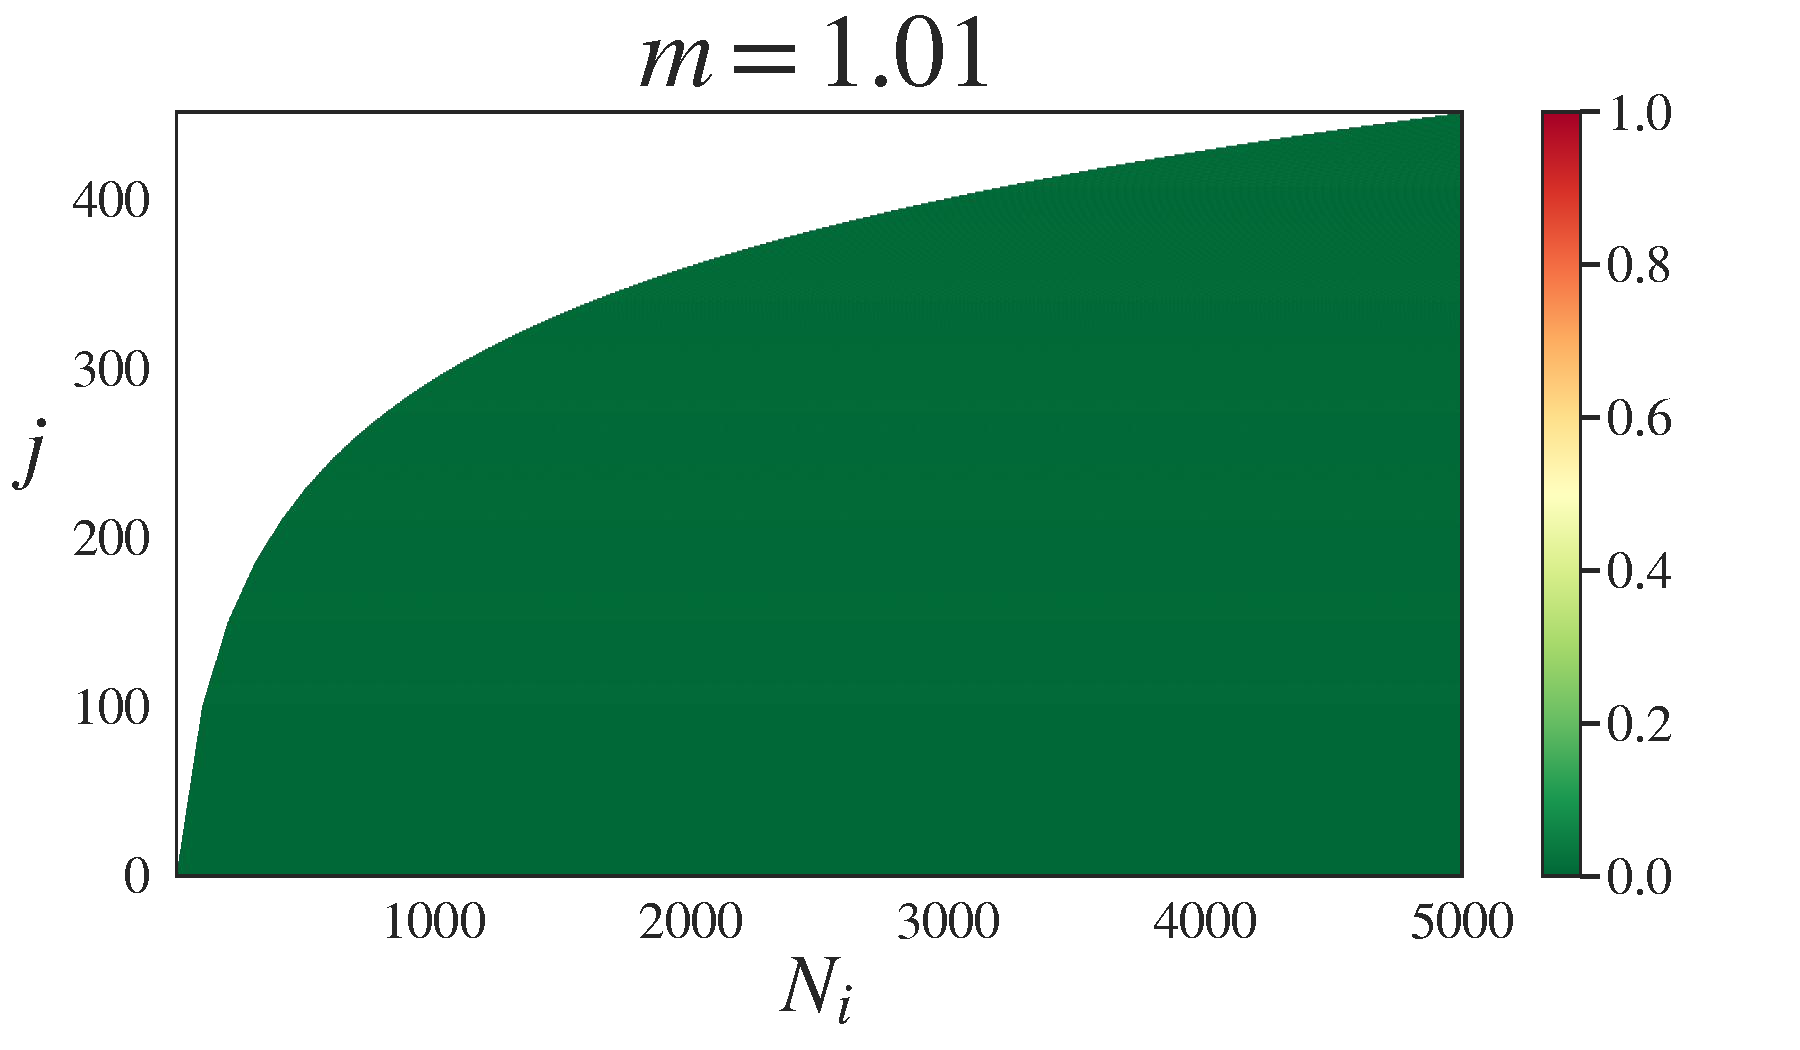
\includegraphics[clip, width= 0.325\textwidth]{2.1Rested/fig/T=5000_m=1,01.pdf}
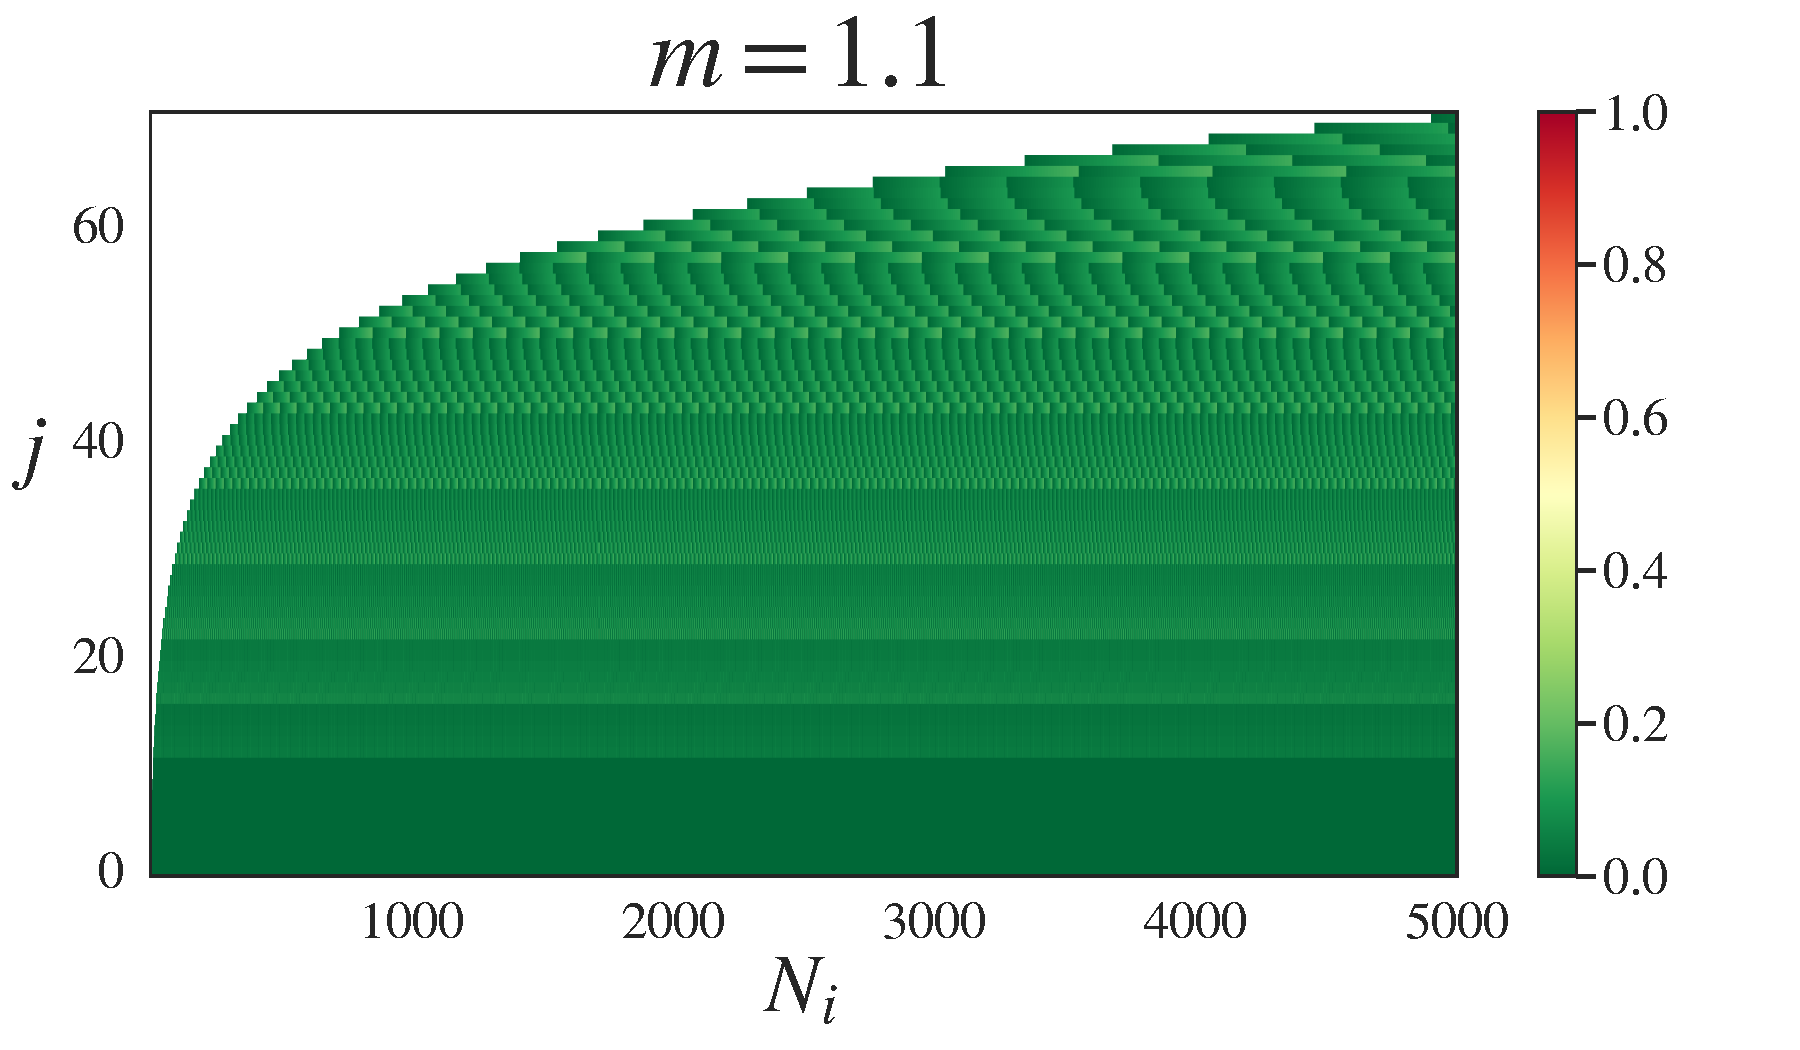
\includegraphics[clip, width= 0.325\textwidth]{2.1Rested/fig/T=5000_m=1,1.pdf}
%\includegraphics[clip, width= 0.325\textwidth]{2.1Rested/fig/T=5000_m=1,2.pdf}
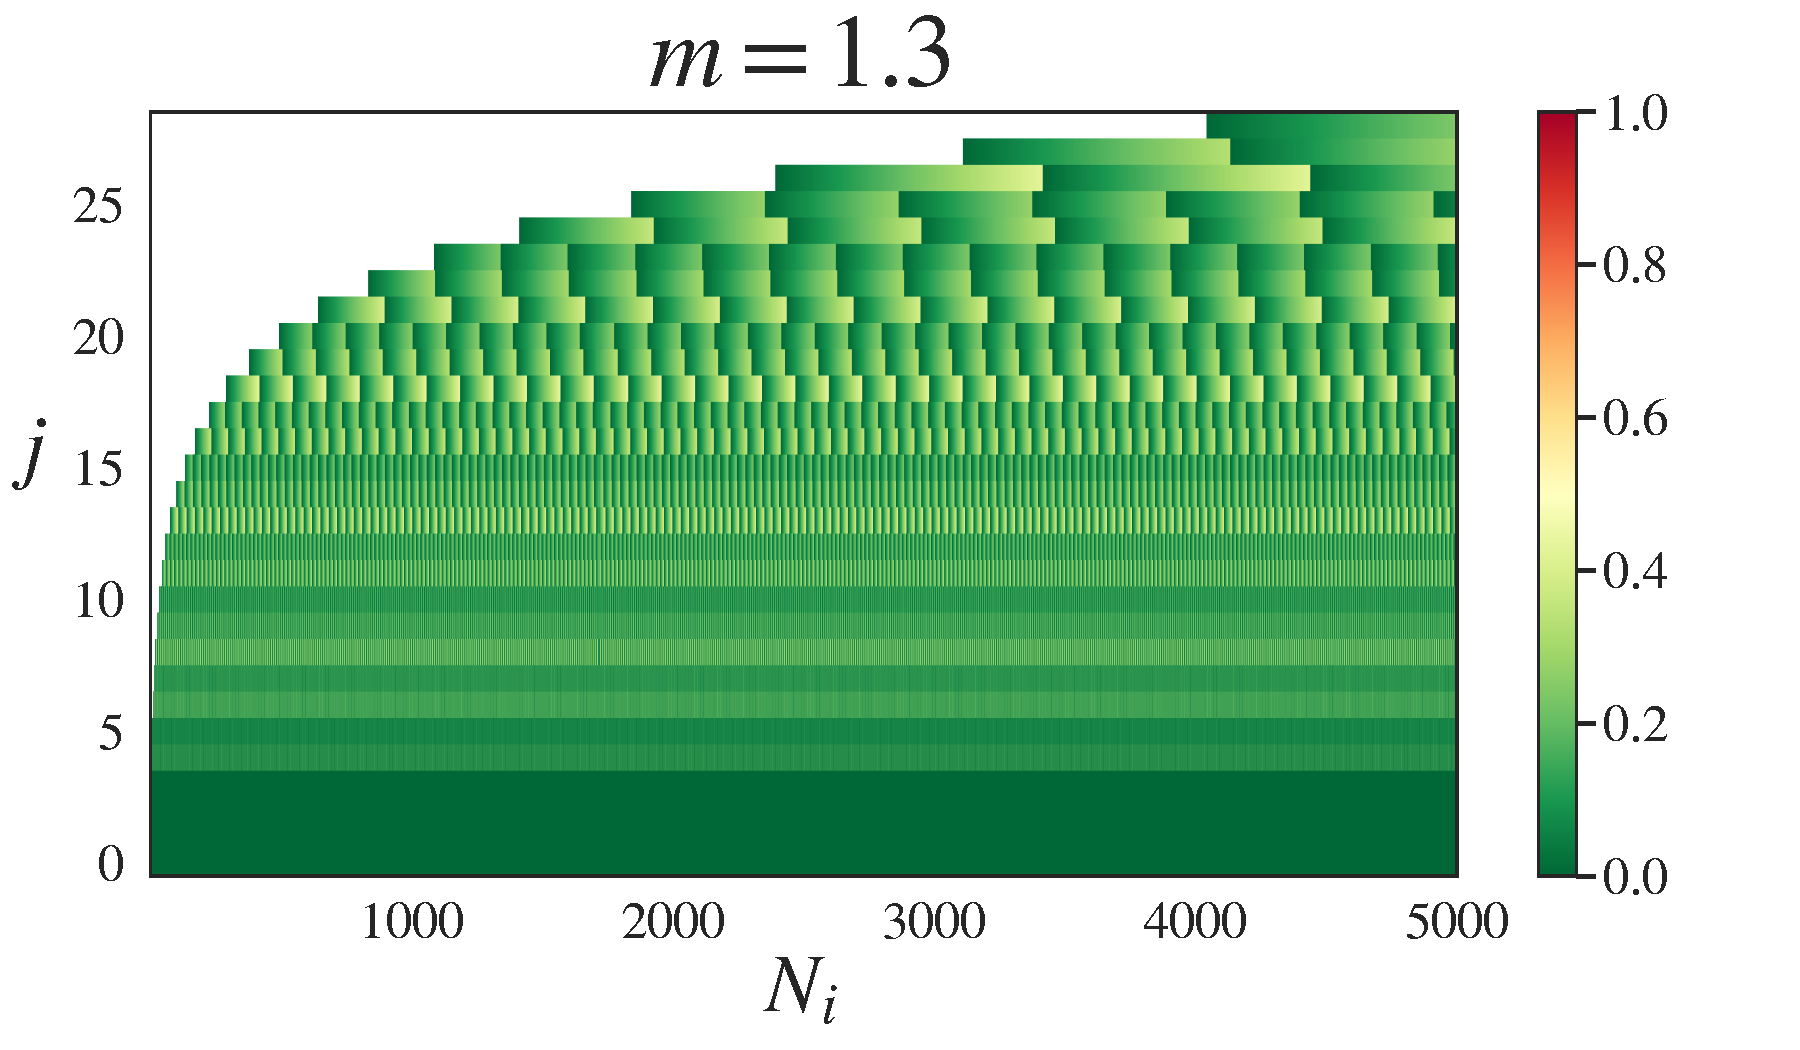
\includegraphics[clip, width= 0.325\textwidth]{2.1Rested/fig/T=5000_m=1,3.pdf}
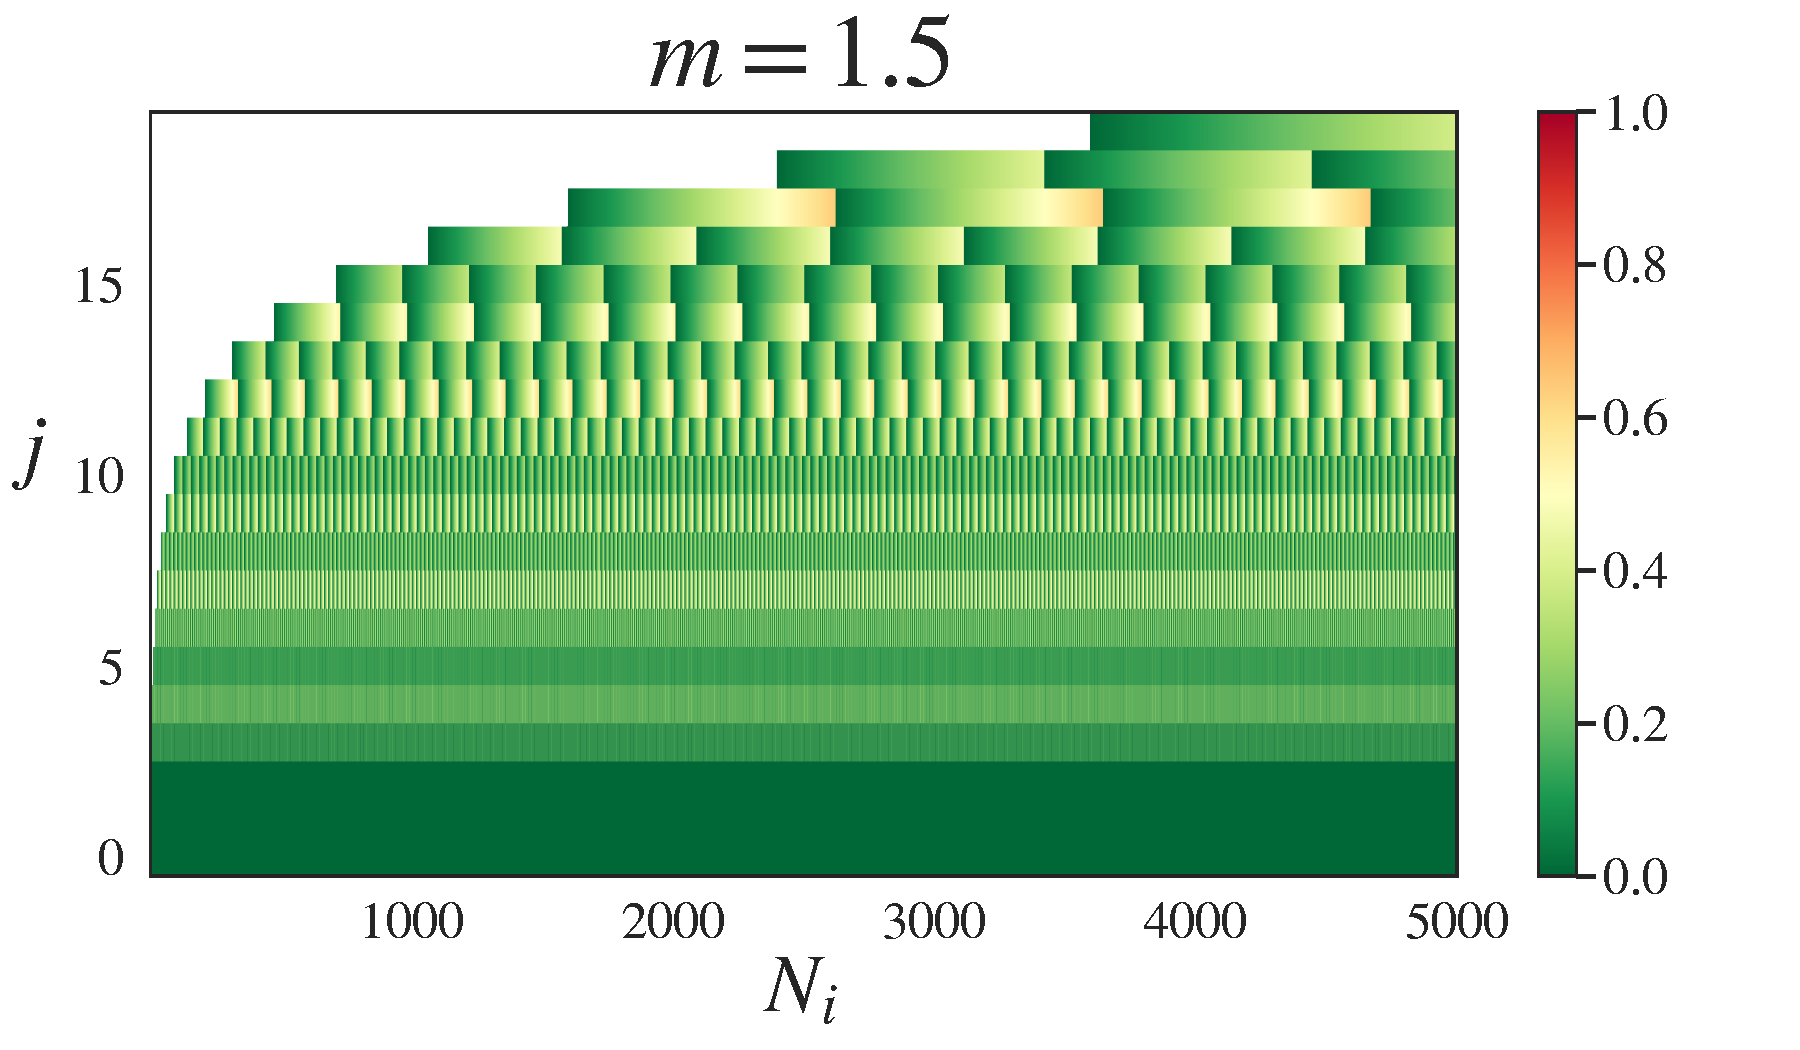
\includegraphics[clip, width= 0.325\textwidth]{2.1Rested/fig/T=5000_m=1,5.pdf}
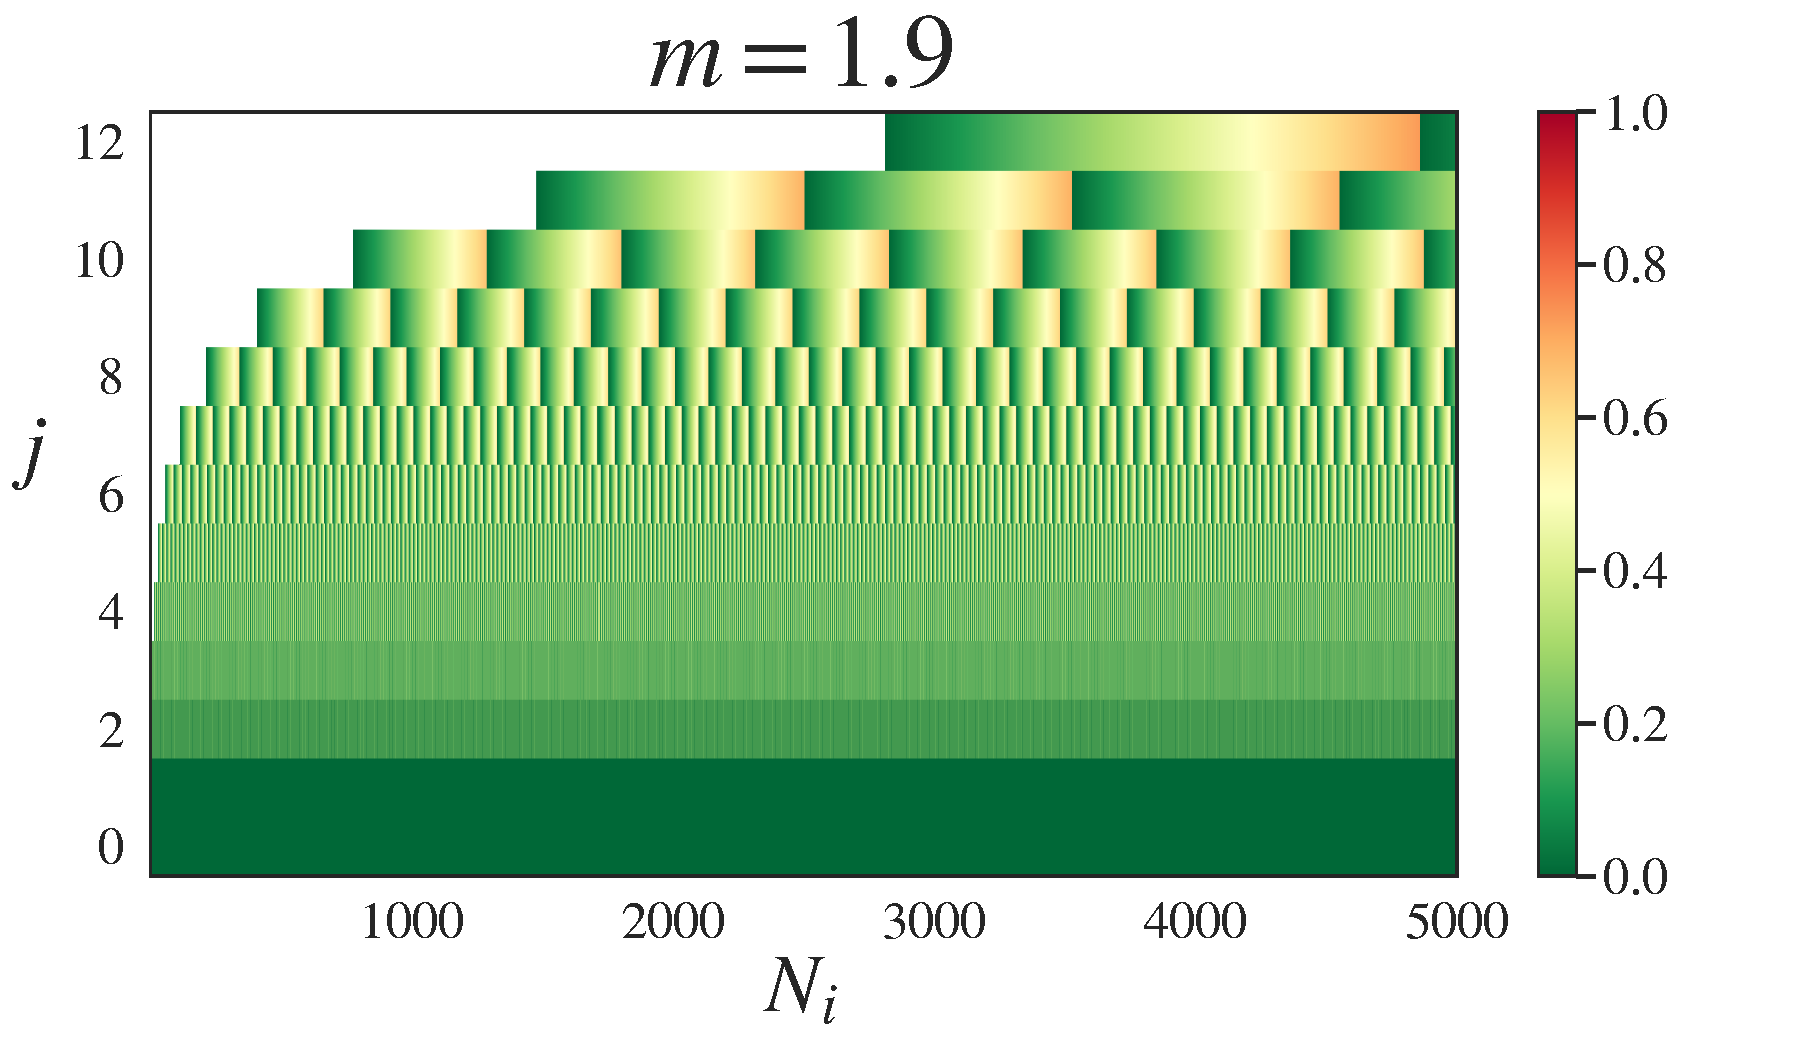
\includegraphics[clip, width= 0.325\textwidth]{2.1Rested/fig/T=5000_m=1,9.pdf}
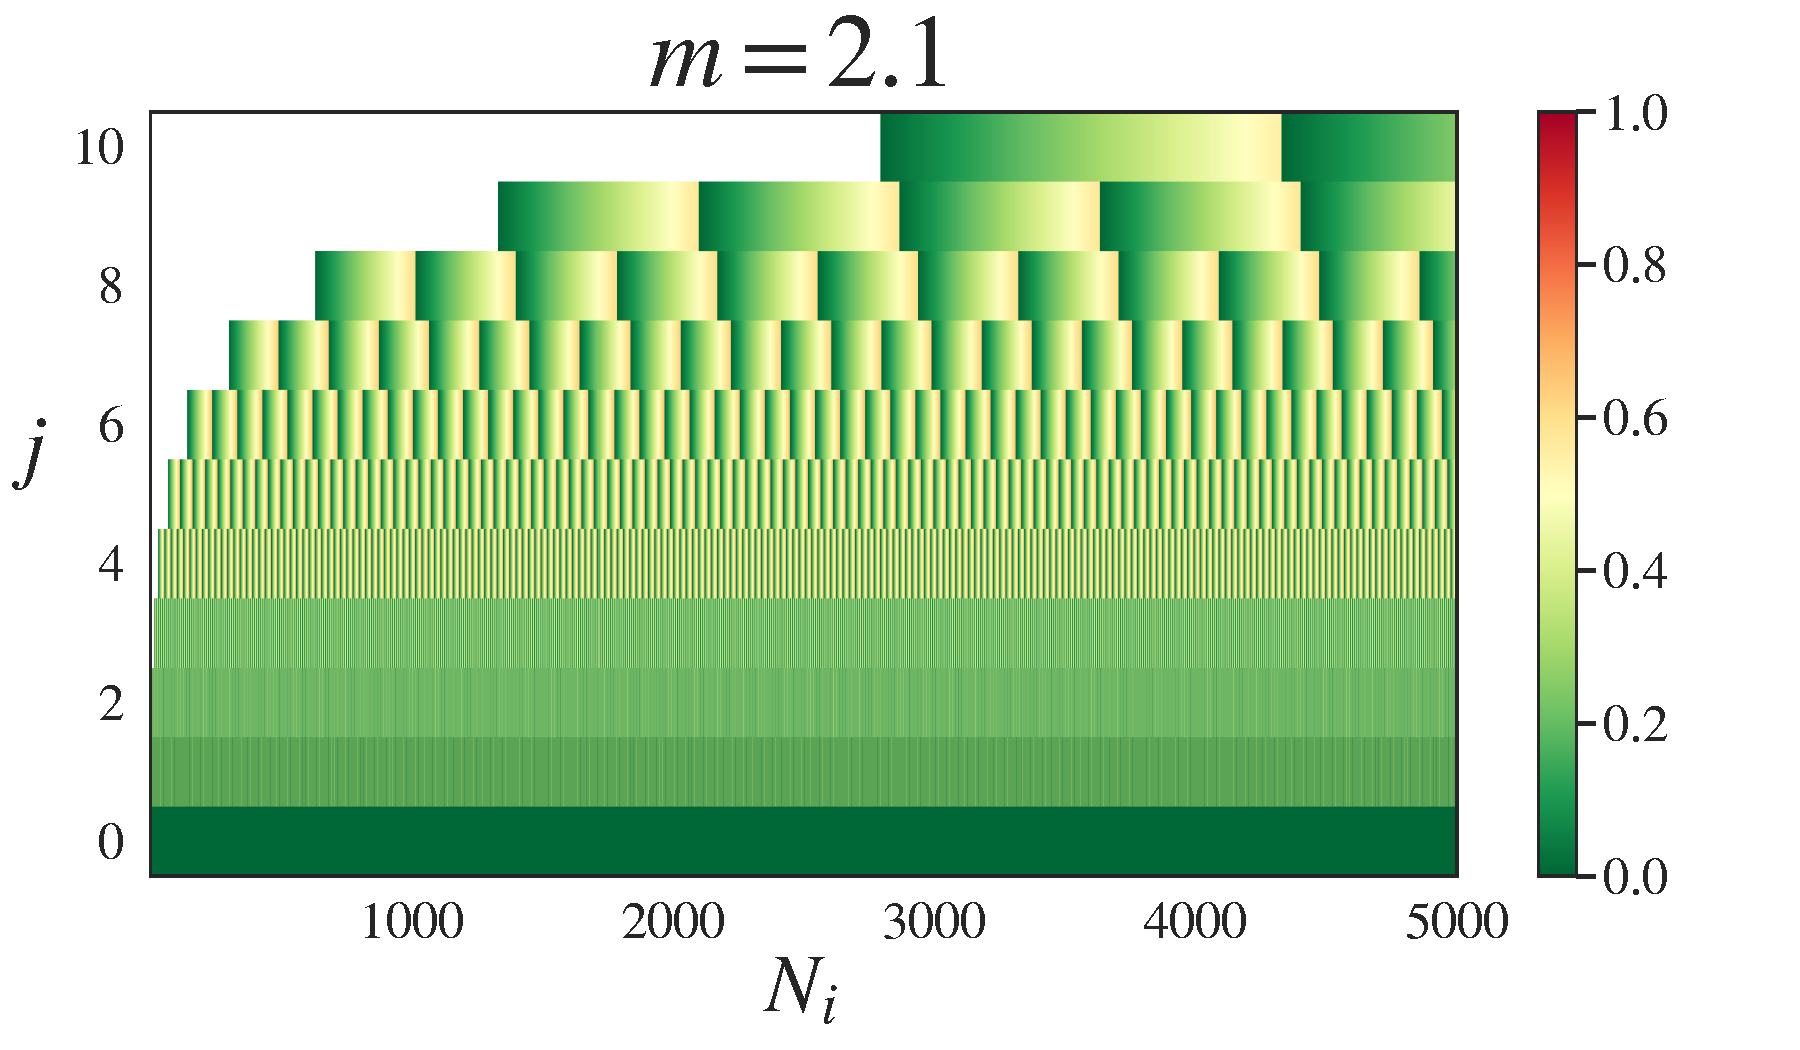
\includegraphics[clip, width= 0.325\textwidth]{2.1Rested/fig/T=5000_m=2,1.pdf}
\caption{Normalized delay $\nicefrac{d_j}{h_j}$ after $N_i$ pulls for each $j$-th statistic $\hmueff$. We display in white the rounds at which statistic $j$ is not created yet.}
\label{fig:delay-general}
\end{figure*}

In Figure~\ref{fig:delay-general}, we display the delay for several non integer values. Compared to the integer case, the update of statistic $j$ does not happen at the same round as the update of statistic $j'<j$. However, we notice that the updates are still periodic and the updating period $\omega_j$ is a multiple of $\omega_{j-1}$. We formalized this properties in Propositions~\ref{prop:effu-delay-periodic} and~\ref{prop:effu-delay-m2} which we show at the end of the Subsection. 

\begin{proposition}
\label{prop:effu-delay-periodic}
For each statistic, the updates are periodic. Moreover, the update period $\omega_{j+1}$ is a multiple of period $\omega_j$,
\[
\omega_{j+1} = \omega_j \pa{1 + \floor{\frac{h_{j+1} - h_{j} -1}{\omega_j}}}.
\]
\end{proposition}

\begin{proposition}
\label{prop:effu-delay-m2}
For $m<2$, $\omega_{j+1}$ is either equal to $\omega_j$ or to $2\cdot \omega_j$. 
\end{proposition}

We notice that this weaker synchronization can lead to a larger normalized delay. Indeed, for $m=2$ the normalized delay is bounded by $50\%$ (Fig.~\ref{fig:delay-int} and Proposition~\ref{prop:effu-delay-int}) while for $m=1.9$ and $m=2.1$ some statistics are delayed by more than $70\%$ (Fig~\ref{fig:delay-general}). Yet, for $m \rightarrow 1$, the normalized delay seems to converge to $0$. Indeed, we prove in Proposition~\ref{prop:effu-delay-ub} that the normalized period cannot exceed twice its minimal value $\nicefrac{m-1}{m}$.

\begin{proposition}
\label{prop:effu-delay-ub}
For $m<2$, either $\omega_j = 1$ or $\omega_j < \frac{2\pa{m-1}}{m} h_j$.
\end{proposition}

Notice that when $\omega_j=1$, there is zero delay in the updates (statistics are updated at every round). We investigate empirically whether this upper-bound is tight. We select ten thousand values of $m$ uniformly at random between $1$ and $2$ and we add the value $m=2$. For each value of $m$, we compute recursively all the $h_j$ and $\omega_j$ (with Proposition~\ref{prop:effu-delay-periodic}) until $h_j > 10^{15}$. Then, we compute the ratio,

 \[r_j \triangleq \frac{m \omega_j}{\pa{m-1}h_j},\] 

for any $j$ such that $\omega_j\neq 1$. According to Proposition~\ref{prop:effu-delay-ub} and Property~\ref{list:effu-delay}, this ratio always lies between $1$ and $2$.

\begin{figure*} 
\centering
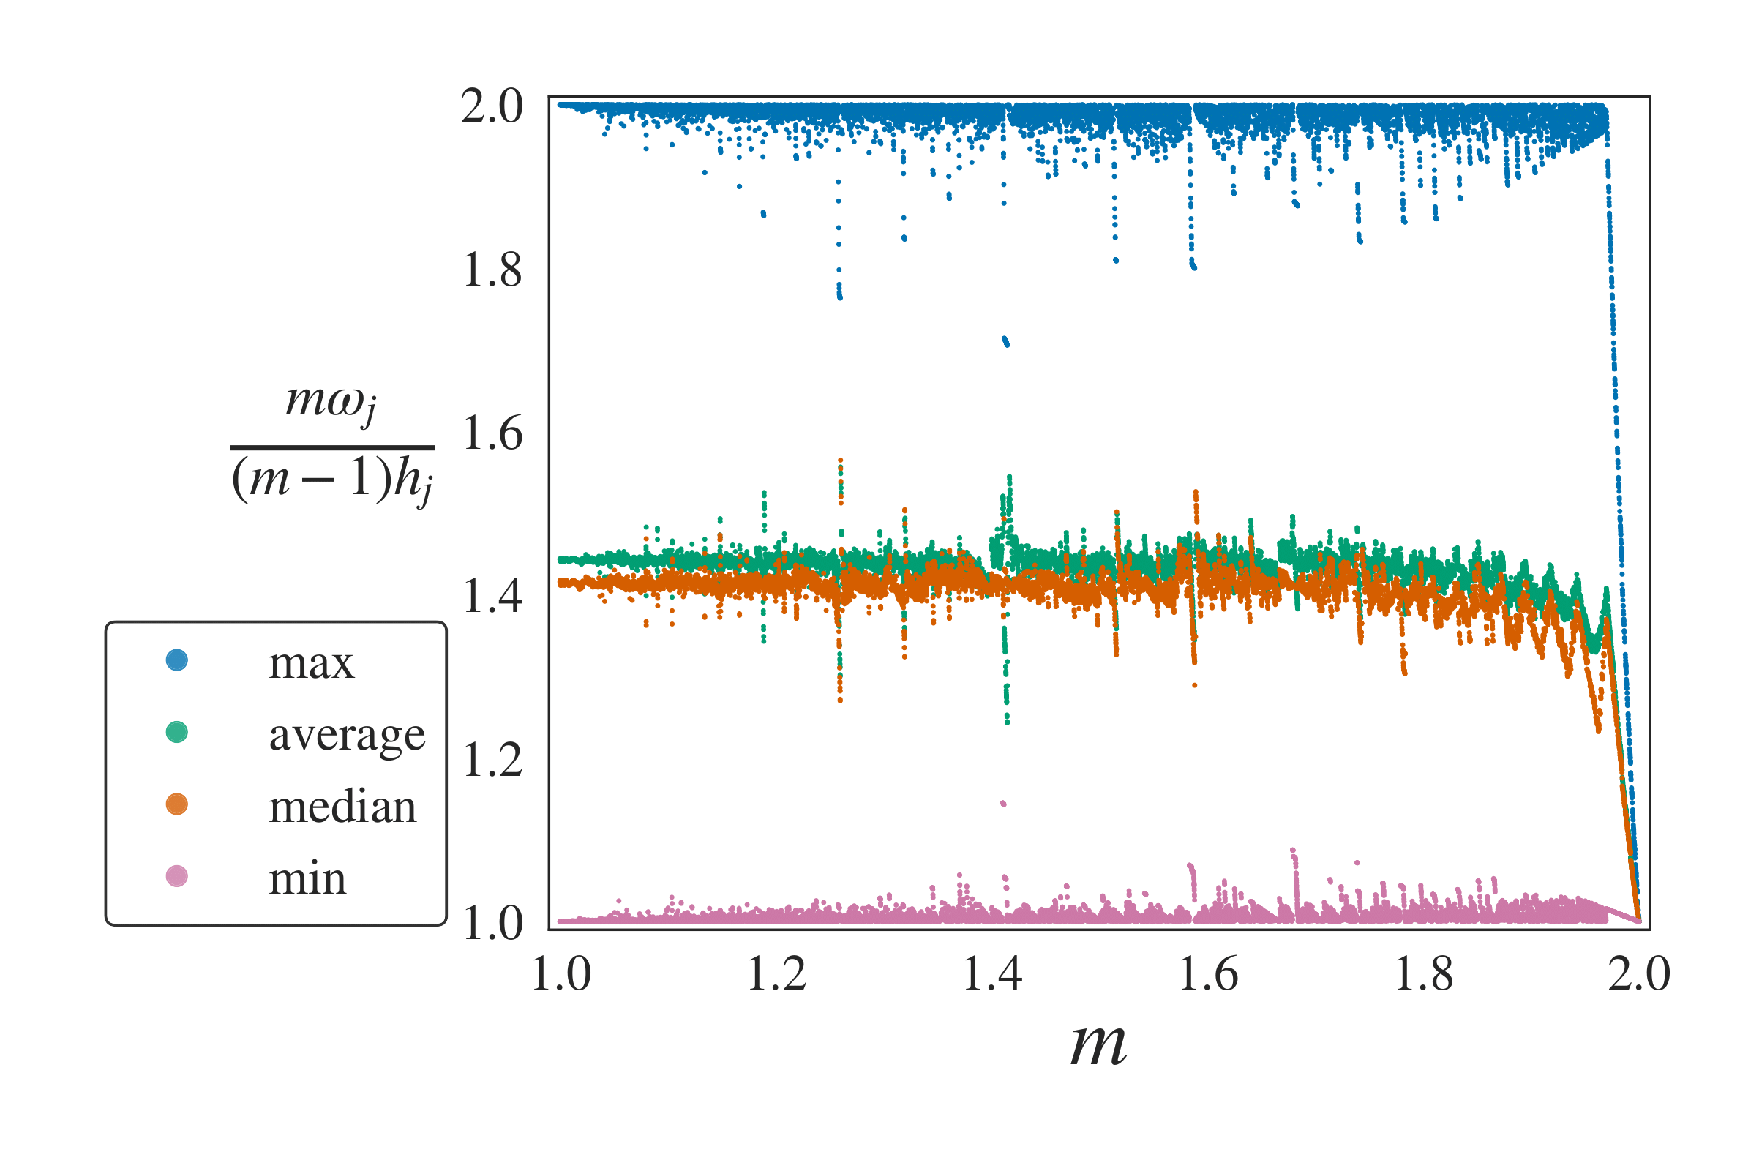
\includegraphics[clip, width= 0.99\textwidth]{2.1Rested/fig/delay_ratio.pdf}
\caption{Impact of $m$ on the minimum, maximum, average and median ratio among $\left\{\nicefrac{m \omega_j}{\pa{m-1}h_j}\right\}_j$.}
\label{fig:delay-ratio}
\end{figure*}

In Figure~\ref{fig:delay-ratio}, we display for each value of $m$ the maximum, minimum, median and average of the sequence $ \left\{ r_j\right\}_j$. Notice that $h_j = 10^{15}$ is much larger than the horizon usually considered in bandits experiments, even to characterize asymptotic performance \citep{chapelle2011empirical, kaufmann2012bayesian, lattimore2018refining}. Hence, the displayed minimum and maximum are valid empirical bounds for real application.

For more than $90\%$ of the values of $m$, the minimum is below $1.02$, the maximum is larger than $1.95$, and the median and mean are between $1.35$ and $1.45$. It shows that our theory is tight in general to characterize the best and worst possible normalized period. 

There are deviations to this general case. First, when $m\rightarrow 2$, the ratio tends to $1$ for all $j$. This is indeed the value when $m=2$. When we compare $m=1.9$ and $m=2$ on Figures~\ref{fig:delay-int} and~\ref{fig:delay-general}, we see that the normalized delay is drifting for $m=1.9$: the updates are synchronous and the normalized delay is $\sim 50 \%$ for the first statistics, but it becomes larger when $j$ is increasing. We conjecture that the closer $m$ is to 2, the slower is the drift.

Second, there are also local deviations (e.g near $m \sim 1.42$). They correspond to values of $m$ such that $m^{k}$ (with $k$ a small integer) is a power of two. In that case, the ratios $\left\{r_j\right\}_j$ are cycling in the regime $h_j >> 1$ (\ie when the rounding effect is negligible and $h_{j+1} \sim m\cdot h_j$)  and take only $k$ values up to small rounding perturbations. These values can either be quite good or quite bad. In fact, due to the rounding, these values are slowly drifting. We can try to control the drift by increasing or decreasing $m$ very slightly to improve the median or the average delay for a given horizon. 

As we can see on Figure~\ref{fig:delay-ratio}, it is very sensitive to the exact value of $m$. For instance, with $\epsilon = 1e^{-5}$,  $m = \pa{1-\epsilon} \times 2^{\nicefrac{1}{3}}$ has an average ratio of $1.29$ while $ m= \pa{1+\epsilon} \times 2^{\nicefrac{1}{3}}$ has an average ratio of $1.55$. Indeed, the normalized delay is not the same for a statistic which is updated just before the precedent one ($r_j \sim 1$) or for one which is updated just after ($r_j \sim 2$) . When the update of $\peff$ is just before, it is refreshed with almost $h_{j-1}$ samples, which is the best possible value. When it is just after, it is refreshed with $\sim h_{j-2}$ which is close to the worse one. Due to this discontinuity, it is hard to take advantage of these local deviation. %For the very long horizon $10^{15}$, we provide in Table~\ref{} interesting values of $m$ associated to local minima of the average of $\left\{r_j\right\}_j$. %TODO ?

To conclude, non-integer values for $m$ leads to a larger ratio $r_j$ than integer values (twice larger in the worst case, $\sim 1.4$ in average). However, the interesting quantity is the normalized period, which is equal to $\nicefrac{\pa{m-1}r_j}{m}$. For $m=2$, the normalized period is $50\%$ for all the statistics $j\geq1$. In order to achieve a lower value in the worst case, one should choose $m\leq \frac{4}{3}$. If we target a lower value in average, one should choose $m\leq 1.56$. It shows that non-integer values are especially interesting when $m\rightarrow 1$. Yet, there is no free lunch: the complexity of \EFFU scales with $\cO\pa{\log_m T}$ which diverges with $\nicefrac{1}{m-1}$ when $m\rightarrow 1$.



\subsubsection{Proofs}
\begin{proof}[Proof of Proposition~\ref{prop:effu-delay-int}]
When $m$ has an integer value, we have, 
\[
h_j = \ceil{m \cdot h_{j-1}} = m \cdot h_{j-1} = \dots = m^j\cdot h_0 = m^j.
\]
For $j=0$, $\hmu_{i,\,\tteff}^1$ is updated at every update at Line~\ref{algline:effu-update-first-hmu}. Hence, $\omega_0 =1$. 
For $j=1$, $h_1 =m$ is initialized after $m$ pulls. At this round, we set $n_i^{h_1}$ to the value in $n_i^{h_0}$ which is equal to $1$. Indeed, the first statistic is always up to date. Hence, the next update is after $m-1$ pulls. At this round, the pending statistics is again refreshed with $p_0$ which contains $1$ sample and, recursively, we can conclude that  $\hmu_{i,\,\tteff}^{h_1}$ is updated every $\omega_1 = m-1 =   \frac{m-1}{m} h_1$.

By induction, let $j$ such that the statistic $j-1$ is updated periodically every $\omega_{j-1} = \pa{m-1} m^{j-2}$ pulls from pull $m^{j-1}$. $\hmueff$ is initialized after $m^j$ pulls (Line~\ref{algline:effu-refresh-hmu}) . It is synchronized with the $m$-th update of statistic $\hmu_{i,\,\tteff}^{h_{j-1}}$. Indeed,
\[ m^j = m \cdot m^{j-1} =  m^{j-1} + m \omega_{j-1}.\]

Notice that we sort $\Him$ in the decreasing order at Line~\ref{algline:effu-refresh-start}, hence $\neff$ is updated with $n_i^{h_{j-1}} = m^{j-1}$ before it is itself refreshed with $n_i^{h_{j-2}}$  (Line~\ref{algline:effu-refresh-n}).  Hence, $\hmueff$ is updated for the first time after $\omega_j =h_{j} - \neff =  m^j - m^{j-1} = (m-1) m^{j-1} = m \omega_{j-1}$ pulls, \ie after $m^{j} + (m-1) m^{j-1}$ pulls of arm $i$. Again, this update is synchronized with the update of the lower order statistic:
\[ m^j +\omega_j =  m^{j} + (m-1) m^{j-1} =  m^{j-1} + 2m \omega_{j-1}.\]
Hence, the pending statistic $\peff$ is again refreshed with $n_i^{h_{j-1}} = m^{j-1}$ sample. Recursively, we can repeat the very same argument and show that $\hmueff$ is updated every $\omega_j = \pa{m-1} m^{j-1}$ pulls from pull $m^{j}$.
\end{proof}

\begin{proof}[Proof of Proposition~\ref{prop:effu-delay-periodic}]
We will prove this property by induction on $j$.  When $j=0$, the updates happen at every round. Hence, $\omega_0 =1$. Let $j$ such that $\hmu_{i,\,\tteff}^{h_{j-1}}$ is refreshed periodically with period $\omega_{j-1}$. $\hmueff$ is initialized after $h_j$ pulls. At that round $\peff$ is initialized with the current value of $p_i^{h_{j-1}}$ which contains $n_i^{h_{j-1}}$ samples. Since statistic $j-1$ is updated with period $\omega_{j-1}$, $n_i^{h_{j-1}}$  takes its value between $h_{j-1} -\omega_{j-1} +1$ and $h_{j-1}$. At pull $h_{j-1}$, it was initialized with value $h_{j-1} -\omega_{j-1} +1$. Then, it is increased by one at every pull and refresh at $h_{j-1} -\omega_{j-1} +1$ when it reaches value $h_j$. Therefore, at pull $h_j$, we have,
\begin{equation}
\label{eq:ni}
n_i^{h_{j-1}}\pa{h_j} = h_{j-1} -\omega_{j-1} +1 + \pa{h_j - h_{j-1} -1  \mod \omega_{j-1}}.
\end{equation}
with $n_i^{h_{j-1}}\pa{h}$, the value of $n_i^{h_{j-1}}$ at the end of the $h$-th pulls of arm $i$. The $-1$ is caused by the backward loop (Line~\ref{algline:effu-refresh-start}: when $h_j -h_{j-1} \mod \omega_{j-1}$, the updates are synchronized such that it minimizes the delay (like in the integer case). The next update of $\hmueff$ will happen in 
\begin{align*} 
\omega_j &\triangleq h_{j} - n_i^{h_{j-1}}\pa{h_j} \\
&= h_{j} - \pa{h_{j-1} -\omega_{j-1} +1 + \pa{h_j - h_{j-1} -1  \mod \omega_{j-1}}} 
\\&= \omega_{j-1} +h_j - h_{j-1} -1 -  \pa{h_j - h_{j-1} -1  \mod \omega_{j-1}} 
\\&=  \omega_{j-1}  \pa{1 + \floor{\frac{h_j - h_{j-1} -1}{\omega_{j-1}}}}
\end{align*}
The second line is justified by Equation~\ref{eq:ni}. The last line uses $a - a\mod b = b \floor{\nicefrac{a}{b}}$. Hence, the first delay $\omega_j$ is a multiple of $\omega_{j-1}$. Therefore, $n_i^{h_{j-1}}\pa{h_j + \omega_j} =n_i^{h_{j-1}}\pa{h_j}$ and $\hmueff$ is refreshed with the same number of sample than its initialization, and the delay until the second update is $h_j - n_i^{h_{j-1}}\pa{h_j + \omega_j} = n_i^{h_{j-1}}\pa{h_j}=\omega_j$. Recursively, we show that  $\hmueff$ is updated periodically with period $\omega_j$.
\end{proof}

\begin{proof}[Proof of Proposition~\ref{prop:effu-delay-m2}]
By \emph{reductio ad absurdum}, we consider the smallest $j\geq 1$ such that  $\omega_{j+1} > 2\cdot \omega_{j}$. A necessary and sufficient condition according to Proposition~\ref{prop:effu-delay-periodic} is that 
\begin{equation}
\label{eq:hj1}
h_{j+1} - h_j -1 \geq  2\omega_j. 
\end{equation}

When $1<m<2$, $h_0=1$, $\omega_0=1$ (as for any $m$), $h_1 = \ceil{m\cdot h_0}  = 2$,  and $\omega_1 = 1$ (according to Prop~\ref{prop:effu-delay-periodic}). Hence, $j \geq 1$.  Since $j\geq 1$ is the smallest value such that $\omega_{j+1} > 2\cdot \omega_{j}$, we have that either $\omega_j = \omega_{j-1}$ or $\omega_j = 2 \cdot \omega_{j-1}$. If $\omega_j = \omega_{j-1}$, we have according to Proposition~\ref{prop:effu-delay-periodic},
\[
h_j - h_{j-1} -1   < \omega_{j-1} = \omega_j. 
\]

If $\omega_j = 2 \cdot \omega_{j-1}$, we have with the same argument, 
\[
h_j - h_{j-1} -1   < 2\cdot \omega_{j-1} = \omega_j. 
\]

Since $h_j$, $h_{j-1}$ and $\omega_j$ are integers, we have 
\begin{equation}
\label{eq:hj2}
 h_j - h_{j-1} -1   < \omega_j \implies h_j - h_{j-1} \leq \omega_j.
 \end{equation}

Using $h_{j+1} = \ceil{m \cdot h_j}$,
\begin{equation}
\label{eq:hj3}
h_{j+1} - h_j -1  = \ceil{m \cdot h_j} - \ceil{m \cdot h_{j-1}} -1 \leq m \pa{h_j - h_{j-1}}
 \end{equation}
 
 Plugging Equations~\ref{eq:hj1}, \ref{eq:hj2} and~\ref{eq:hj3}, 
 \[ m \pa{h_j - h_{j-1}} \geq 2\pa{h_j - h_{j-1}}. \]

This is impossible for $m<2$ and $h_j > h_{j-1}$ (which is the case when $m>1$).  Hence, we conclude that there exists no integer $j$ such that $\omega_{j+1} > 2 \cdot \omega_j$.

\end{proof}

\begin{proof}[Proof of Proposition~\ref{prop:effu-delay-ub}]
We want to upper bound the ratio $\nicefrac{\omega_j}{h_j}$ for all $j$ such that $\omega_j>1$.  When $m < 2$ we have either $\omega_{j} = \omega_{j-1} $ or $\omega_{j} = 2 \cdot \omega_{j-1}$ (Prop.~\ref{prop:effu-delay-m2}). We first study the case where $\omega_{j} = 2 \cdot \omega_{j-1}$, \ie (Prop;~\ref{prop:effu-delay-periodic}),
\[
h_j - h_{j-1} - 1 \geq \omega_{j-1} = \nicefrac{\omega_{j}}{2}.
\]

Using $h_j = \ceil{m\cdot h_{j-1}}\implies h_{j-1} = \floor{\nicefrac{h_j}{m}}$, 
\[
h_j - h_{j-1} - 1 = h_j - \floor{\nicefrac{h_j}{m}} - 1  \leq \frac{m-1}{m} h_j.
\]

Plugging the two last equations leads to, 
\[
\frac{\omega_j}{h_j} \leq \frac{2 \pa{m-1}}{m}\cdot
\]


We notice that $\left\{h_j\right\}_{j \in \NN}$ is an increasing sequence. When $\omega_{j} = \omega_{j-1}$,  we have $\nicefrac{\omega_{j}}{h_j} < \nicefrac{\omega_{j-1}}{h_{j-1}}$. Therefore, for any $j$ such that $d_j > 1$ we can find the largest $j'\leq j$ such that $\omega_{j'} = 2 \cdot \omega_{j'-1}$ and compare, 
\[
\frac{\omega_j}{h_j} \leq \frac{\omega_j}{h_j'} = \frac{\omega_j'}{h_j'} \leq \frac{2 \pa{m-1}}{m}\cdot
\]
\end{proof}

\subsection{{\EFFFEWA} ($\piEF$) and {\EFFRAW} ($\piER$)}
{\EFFFEWA} ($\piEF$) and {\EFFRAW} ($\piER$) are the two efficient versions of our initial algorithms. With an hyperparameter $m>1$, they use \EFF instead of \UPDATE (Lines~\ref{algline:fewa-update1} and~\ref{algline:fewa-update2} in \FEWA and Lines~\ref{algline:raw-update1} and~\ref{algline:raw-update2} in \RUCB). Therefore, they use $\left\{\hmueff\right\}_{i,h_j\in \Him}$ instead of $\left\{\hmu_i^h\right\}_{i,h \leq \Nitmone}$. 

More precisely, in \FEWA, we replace the increment $h\gets h+1$ by $h\gets\ceil{m\cdot h}$ at Line~\ref{algline:fewa-window}. Hence, the next set is not called $\arms_{h+1}$ but $\arms_{\ceil{m\cdot h}}$ (Line~\ref{algline:fewa-filter} in \FEWA and Line~\ref{algline:filter-add} in \FILTER). Finally, at Lines~\ref{algline:fewa-condition} and~\ref{algline:fewa-pull}, the condition is not $N_{i_t}=h$ but $N_{i_t} \leq h$. In the \FILTER procedure, we also change $\hmu_i^h$ by $\hmu_{i,\,\tteff}^h$ at Lines~\ref{algline:filter-max} and~\ref{algline:filter-delta}. In \RUCB, we only change the $h\leq N_i$ by $h_j \in \Him$ and $\hmu_i^h$ by $\hmueff$ in the index computation at Line~\ref{algline:raw-pull}.

\begin{proposition}
At any round $t$, \EFFFEWA and \EFFRAW tuned with hyperparameter $m$ have a $\cO\pa{K\log_m\pa{t}}$ worst-case time and space complexity.
\end{proposition}
\begin{proof}
For each arm, the algorithms use the statistics created and maintained by \EFFU plus a handful of variables (such as $t$). Hence, the space complexity is the sum of the complexities of \EFFU (see Prop.~\ref{prop:effu-complexity}) for each arm, \ie

\[ 
\sum_{i \in \arms} \cO\pa{\log_m\pa{\NiT}}\leq \cO\pa{K\log_m\pa{T}}.
\] 

At every round $t$, the algorithms do one call of \EFFU, which costs at most $\cO\pa{\log t}$. For each of the $\cO\pa{K\log_m t}$, \EFFRAW computes one ucb with unit cost $\cO\pa{1}$. For each of the $K$ arms, we find the minimum ucb among the $\cO\pa{\log_m t}$ ones. It costs $\cO\pa{K\log_m t}$ in total. Finally, we select the arm with the largest index, which costs $\cO\pa{K}$. Hence, the worst-case time complexity at any round $t$ is $\cO\pa{K\log_m t}$.

\EFFFEWA uses the procedure \FILTER  at most for each existing window, \ie $\cO\pa{\log_m\pa{t}}$. The inner time complexity of \FILTER scales with $|\arms_h| \leq K$. Therefore, in the worst case, the time complexity of \EFFFEWA at any round $t$ is also bounded by $\cO\pa{K\log_m\pa{t}}$.
\end{proof}

\subsection{Regret analysis}
In our analysis, the particularities of \RAWUCB and \FEWA only appear in Proposition~\ref{prop:prb_favorable_event} and Corollary~\ref{cor:core-RAW-FEWA}. We will derive analogous results for \EFFRAW and \EFFFEWA when $m=2$. The upper-bounds will directly follow with no additional effort. We discuss the case $m\neq 2$ at the end of this Subsection. 
\paragraph{A favorable event for efficiently updated adaptive windows}
\begin{proposition}
\label{prop:prb_favorable_event_eff}
For any round $t$ and confidence $\delta_{t} \triangleq 2t^{-\alpha}$, let 
%
\begin{equation*}
\!\HPeff\! \triangleq\! \Big\{ \forall i\!\in\!\arms,\ \forall n \!\leq\! t\!-\!1 ,\ \forall h_j \in \Him(n), \big| \hmueff(t, \pi) - \bmueff(t,\pi) \big| \!\leq\! c(h_j, \delta_{t}) \!\Big\}
\end{equation*}
 be the event under which the estimates at a round $t$  are all accurate up to $c(h,\delta_{t}) \triangleq \sqrt{2 \subgaussian^2\log(2/\delta_t)/h}$. Then, for a policy $\pi$ which pulls each arms once at the beginning, and for all $t>K$,
\[
\PPempty\Big[\bar{\HPtwo}\Big] \leq 3Kt\delta_t= 6Kt^{1-\alpha}\,\cdot
\]
\end{proposition} 
\begin{remark}
The probability of the unfavorable event $\bar{\HPtwo}$ scales with $\cO\pa{t^{1-\alpha}}$ compared to $\cO\pa{t^{2-\alpha}}$ for $\bar{\HPevent}$ because the efficient algorithms construct less statistics. It means that our theory will hold for a wider range of $\alpha$. Yet, this benefits is only theoretical. The union bound in Proposition~\ref{prop:prb_favorable_event} is not tight because the different events share the same data. In practice, it leads to conservative tuning of the confidence bounds and one can decrease $\alpha$ to get better performance. 
\end{remark}

\begin{proof}
As in Propositions~\ref{prop:prb_favorable_event_SWA} and~\ref{prop:prb_favorable_event}, we have to count the number of statistics that are required to hold in the confidence region. 
We call  $u_j(n)$ the number of different values taken by variable $\hmueff$ after $t$. According to Proposition~\ref{prop:effu-delay-int}, $u_0(n) = n \leq t $ because statistic $0$ is created at the first round and updated at every round ($\omega_0=1$). For $m=2$ and $j\geq 1$,  $\hmueff$ is created after $h_j= 2^j$ pulls and then updated every $\omega_j = 2^{j-1}$. Hence, 
\[
\forall j \geq 1 \text{ and } h_j \leq n, u_j(n) = 1 + \floor{\frac{n-h_j}{\omega_j}} \leq \frac{n}{2^{j-1}} - 1 \leq \frac{n}{2^{j-1}}\cdot
\]

We do the union bound, 
\begin{align*}
    \PPempty\Big[\bar{\HPtwo}\Big] &\leq \sum_{i \in \arms} \sum_{j=0}^{|\Him(\Nit)|} u_j(t) \delta_t \\
    &\leq \sum_{i \in \arms} \pa{t  + \sum_{j=1}^{|\Him(\Nit)|} \frac{t}{2^{j-1}}} \delta_t \\
    &\leq 3Kt\delta_t.
\end{align*}
\end{proof}

\begin{lemma}
\label{lem:core-eff}
At any round $t$ on favorable event $\HPtwo$, if arm~$i_{t}$ is selected by $\pi \in \left\{\piEF, \piER\right\}$ tuned with $m=2$, for any $h \leq \Nitmone$,  the average of its $h$ last pulls cannot deviate significantly from the best available arm at that round, i.e.,
\begin{equation*}
\bmu^{h}_{i_t}(t-1,\pi) \geq \max_{i \in \arms} \mu_{i}(t,\Nitmone)- \frac{C_\pi}{\sqrt{2\alpha}} c(h, \delta_t) \quad \text{with } 
\begin{cases}
C_{\piER} = \frac{4\sqrt{\alpha}}{\sqrt{2}-1}\\
C_{\piEF} = \frac{8\sqrt{\alpha}}{\sqrt{2}-1}
\end{cases}\cdot
\end{equation*}
\end{lemma}

\begin{proof}
Like for Lemma~\ref{lem:core-FEWA} (see its proof), our proof is done in a more general rotting framework that can be used in the next chapter. We denote by $\bar{\mu}^{hh'}_i(t-1,\pi)$ and $\hat{\mu}^{hh'}_i(t-1,\pi)$ the true mean and empirical average associated to the $h'-h$ samples between the $h$-th last one (included) and the $h'$-th last one (excluded). Let $j_h \in \NN^\star$ such that:
$2^{j_h} -1 \leq  h < 2^{j_h+1}$.
\begin{equation}
\label{eq:eff-decompo}
\bar{\mu}^{h}_{i_t}(t-1,\pi) \geq \bar{\mu}^{2^{j_h}-1}_{i_t}(t, \pi) = \sum_{j=0}^{j_h-1} \frac{2^j}{2^{j_h}-1} \bar{\mu}^{2^{j}2^{j+1}}_{i_t}(t, \pi).
\end{equation}
The inequality follows because the reward is decreasing and $h\geq 2^{j_h}-1$. Then, we decompose the average in a weighted sum of averages of geometrically expanding windows. Since the reward is decreasing we have that,
\begin{equation*}
\forall k \leq 2^j, \quad \bar{\mu}^{2^{j}2^{j+1}}_{i_t}(t, \pi) \geq \bar{\mu}^{k : k+2^{j}}_{i_t}(t, \pi).
\end{equation*}

$\hmuiteff$ contains $2^j$ samples among the $2^{j+1}-1$ last ones (see Proposition~\ref{prop:effu}). Setting $k\leq 2^j$ to the current delay of the statistics $\hmuiteff$ (see Point~\ref{list:effu-delay} in Proposition~\ref{prop:effu}), we can write,

\begin{equation}
\label{eq:hmueff-link}
\bar{\mu}^{2^{j}2^{j+1}}_{i_t}(t, \pi) \geq \bar{\mu}^{k : k+2^{j}}_{i_t}(t, \pi) = \bmuiteff\geq  \hmuiteff - c(2^j, \delta_t),
\end{equation}
where we use that we are on $\HPtwo$ for the last inequality. Therefore, gathering Equations~\ref{eq:eff-decompo} and~\ref{eq:hmueff-link}, 
\begin{equation}
\label{eq:eff-general}
\bar{\mu}^{h}_{i_t}(t, \pi) \geq \sum_{j=0}^{j_h-1} \frac{2^j}{2^{j_h}-1} \pa{\hmuiteff - c(2^j, \delta_t)}.
\end{equation}
Now, we will use the mechanics of the two algorithms. On the first hand, for $\EFFRAW$, we make the index appear in the inequality,
\begin{align}
 \bar{\mu}^{h}_{i_t}(t, \piER) &\geq \sum_{j=0}^{j_h-1} \frac{2^j}{2^{j_h}-1} \pa{\hmuiteff - c(2^j, \delta_t)} \nonumber\\
 &=\sum_{j=0}^{j_h-1} \frac{2^j}{2^{j_h}-1} \pa{\hmuiteff + c(2^j, \delta_t) - 2c(2^j, \delta_t)}\nonumber\\
 &\geq \min_{j \in H_{i_t, 2}} \pa{\hmuiteff + c(2^j, \delta_t)} - 2 \sum_{j=0}^{j_h-1} \frac{2^{j}}{2^{j_h}-1} c(2^j, \delta_t).
 \label{eq:effraw-index-appear}
 \end{align}
 %
 Then, we can relate the left part of the sum to the best current value $\mu_{\ist}(t,\Nisttmone)$,
 \begin{equation}
 \min_{j \in H_{i_t, 2}}  \pa{\hmuiteff + c(2^j, \delta_t)} \geq \min_{j \in H_{\ist,2}} \pa{\hmu_{\ist,\, \tteff}^{h_j} + c(2^j, \delta_t)}\geq  \bmu_{\ist,\, \tteff}^{h_{\min}} \geq \mu_{\ist}(t,\Nisttmone).
 \label{eq:effraw-index-use}
 \end{equation}
%
where $h_{\min} \in \argmin_{h_j \in H_{\ist,2}} \pa{\hmu^{h_j}_{\ist,\, \tteff} + c(h_j, \delta_t)}$.The first inequality follows because \EFFRAW selects the arm $i_t$ with the largest index. In particular, the index of $i_t$ is larger or equal to the index of $i^\star_t \in \argmax_{i\in \arms} \mu_i(t, N_{\ist,\,t})$. The second inequality holds on $\HPtwo$. The third inequality uses the decreasing of the reward. Putting Equations~\ref{eq:effraw-index-appear} and~\ref{eq:effraw-index-use}, we get,
\begin{equation}
\label{eq:effraw-result}
\bmu^{h}_{i_t}(t, \piER) \geq \mu_{\ist}(t,\Nisttmone)- 2 \sum_{j=0}^{j_h-1} \frac{2^{j}}{2^{j_h}-1} c(2^j, \delta_t).
\end{equation}
%
On the other hand, for \EFFFEWA, we know that the selected arm passes any filter of window $2^j \in H_{i_t, 2}$. Therefore, with $i_{\max} \in \argmax_{i \in \arms_{h_j}} \bmueff$, we can write,
\begin{flalign}
\qquad\hmuiteff &\geq \max_{i\in \arms_{h_j}} \hmueff -2c\pa{h_j, \delta_t} \nonumber && \text{Filtering rule}\\
\qquad&\geq \hmu_{i_{\max}, \, \tteff}^{h_j}  -2c\pa{h_j, \delta_t} \nonumber  && i_{\max} \in \arms_{h_j} \\
\qquad&\geq \bmu_{i_{\max}, \, \tteff}^{h_j} - 3c(h_j, \delta_t)\nonumber && \text{ on }\HPtwo \\
\qquad& = \max_{i\in \arms_{h_j}}  \bmueff -3c\pa{h_j, \delta_t}.
\label{eq:efffewa-3c}
\end{flalign}
%
We relate $\bmueff$ to the largest available value at the round $t$,
\begin{equation}
\label{eq:efffewa-ist-relation}
\max_{i\in \arms_{h_j}} \bmueff \geq \max_{i\in \arms_{1}}\bmu_{i,\tteff}^1 =  \max_{i\in \arms}\bmu_{i,\tteff}^1 \geq \bmu_{\ist,\tteff}^1 \geq  \mu_{\ist}(t, \Nisttmone).
\end{equation}
%
The last inequality follows from the decreasing of the reward and the before last from the definition of the maximum operator. The first one uses a similar argument than in Lemma~\ref{lem:core-FEWA}: $\max_{i\in \arms_{h_j}} \bmueff$ increases with $h_j$.  Indeed, on $\HPtwo$, 
\[  i_j \in \argmax_{i\in \arms_{h_j}} \bmueff \subset \arms_{h_{j+1}},\]
 because it cannot be at more than two confidence bounds from the best empirical value during the filter $h_j$. Thus, we get, 
\[
\max_{i\in \arms_{h_j}} \bmueff = \bmu_{i_j,\tteff}^{h_j} \leq \bmu_{i_j,\tteff}^{h_{j+1}} \leq \max_{i\in \arms_{h_{j+1}}}\bmu_{i,\tteff}^{h_{j+1}}. 
\]
The first inequality follows because $\bmu_{i_j,\tteff}^{h_{j+1}}$ contains reward sample which are either in $\bmu_{i_j,\tteff}^{h_j}$ or are older than the ones in $\bmu_{i_j,\tteff}^{h_j}$. Indeed, when $m=2$, $\hmu_{i, \, \tteff}^{h_{j+1}}$ is updated synchronously with $\hmueff$ (see Figure~\ref{fig:delay-int} and its section on delay). Hence, at each update of $\hmu_{i, \, \tteff}^{h_{j+1}}$, it contains all the samples of $\hmueff$ and the $2^j$ precedent ones. Thus, because the reward is decreasing, we have $\bmu_{i_j,\tteff}^{h_{j+1}} \geq \bmu_{i_j,\tteff}^{h_{j}} $.  The second inequality uses that $i_j \in \arms_{h_{j+1}}$. Gathering Equations~\ref{eq:eff-general}, \ref{eq:efffewa-3c} and~\ref{eq:efffewa-ist-relation}, we get 
%
\begin{equation}
\label{eq:efffewa-result}
\bmu^{h}_{i_t}(t, \piEF) \geq  \mu_{\ist}(t,\Nisttmone)- 4 \sum_{j=0}^{j_h-1} \frac{2^{j}}{2^{j_h}-1} c(2^j, \delta_t).
\end{equation}
%
With few lines of algebra, we reduce the sum,
\begin{flalign*}
\sum_{j=0}^{j_h-1} \frac{2^{j}}{2^{j_h}-1} c(2^j, \delta_t) &= \sum_{j=0}^{j_h-1} \frac{\sqrt{2}^{j}}{2^{j_h}\!-\!1} c(1, \delta_t) && c(2^j, \delta_t) = \frac{c(1,\delta_t)}{\sqrt{2^j}} \\
& = \frac{\sqrt{2}^{j_h} -1 }{\pa{\sqrt{2}-1}\pa{2^{j_h}-1}}c(1, \delta_t) && \sum_{n=0}^N q^n = \frac{q^{N+1}-1}{q-1}\\
& = \frac{1}{\pa{\sqrt{2}-1}\pa{\sqrt{2}^{j_h}+1}} c(1, \delta_t) && a^2\!-\!1 \!=\!  \pa{a\!-\!1}\!\pa{a\!+\!1}\\
& \leq  \frac{\sqrt{2}}{\pa{\sqrt{2}-1}\sqrt{2^{j_h+1}}} c(1, \delta_t) &&\sqrt{2^{j_h}} +1 \geq  \frac{\sqrt{2^{j_h+1}} }{\sqrt{2}} \\
& \leq \frac{\sqrt{2}}{\pa{\sqrt{2}-1}\sqrt{h}} c(1, \delta_t) &&  h \leq 2^{j_h+1}  \\
& = \frac{\sqrt{2}}{\sqrt{2}-1} c(h, \delta_t). &&  \frac{c(1,\delta_t)}{\sqrt{h}} = c(h, \delta_t)
%& \leq \frac{\sqrt{2}}{\sqrt{2}-1} c(h, \delta_t). && }  c(\cdot, \delta) \searrow
\end{flalign*}
%
Plugging this last equation in Equations~\ref{eq:effraw-result} and~\ref{eq:efffewa-result} leads to the final result,
\[
\bmu^{h}_{i_t}(t, \pi) \geq \max_{i \in \arms} \mu_{i}(t,\Nitmone)- \frac{C_\pi}{\sqrt{2\alpha}} c(h, \delta_t) \quad \text{with } 
\begin{cases}
C_{\piER} = \frac{4\sqrt{\alpha}}{\sqrt{2}-1}\\
C_{\piEF} = \frac{8\sqrt{\alpha}}{\sqrt{2}-1}
\end{cases}\cdot
\]
\end{proof}
Using Proposition~\ref{prop:prb_favorable_event_eff} and Lemma~\ref{lem:core-eff} instead of Prop.~\ref{prop:prb_favorable_event} and Corollary~\ref{cor:core-RAW-FEWA}, we can obtain similar problem dependent and independent bounds than for \FEWA and \RUCB. The proof directly follows from the precedent analysis. 
\begin{theorem}
\label{th:rested-PI-eff}
For any rotting bandit scenario with means $\{\mu_i\}_{i} \in \rewardSet^K$ and any time horizon $T$, $\pi \in \left\{\piER, \piEF \right\}$ run with $\alpha \geq 4$ and $m=2$ suffers an expected regret of
\begin{equation*}
\mathbb{E}[\regret(\pi)] \leq C_\pi\sigma \sqrt{\log\pa{T}}\pa{\sqrt{KT} +K} + 6KL \;\; \text{with } 
\begin{cases}
C_{\piER} = \frac{4\sqrt{\alpha}}{\sqrt{2}-1}\\
C_{\piEF} = \frac{8\sqrt{\alpha}}{\sqrt{2}-1}
\end{cases}\cdot
\end{equation*}
\end{theorem}
\begin{theorem}\label{th:rested-PD-eff}
For any rotting bandit scenario with means $\{\mu_i\}_{i} \in \rewardSet^K$ and any time horizon $T$, $\pi \in \left\{\piER, \piEF \right\}$ run with $\alpha \geq 4$ and $m=2$ suffers an expected regret of
\begin{align*}
\mathbb{E}\left[R_T(\pi)\right]  \leq \sum_{i\in \arms} \pa{\frac{C_\pi^2\sigma^2\log\pa{T}}{\Delta_{i,\hiT^+-1}} +  C_\pi\sigma\sqrt{\log\pa{T}} +6L } \\
\text{with } 
\begin{cases}
C_{\piER} = \frac{4\sqrt{\alpha}}{\sqrt{2}-1}\\
C_{\piEF} = \frac{8\sqrt{\alpha}}{\sqrt{2}-1}\\
\text{$\Delta_{i,h}$ and $\hiT^+$ defined in Equation~\ref{eq:hit+}.}
\end{cases}
\end{align*}
\end{theorem}
Among the differences, we notice that our theory holds for a larger range of $\alpha \geq 4$ but the constant $C_\pi$ is $\frac{\sqrt{2}}{\sqrt{2}-1} \sim 3.4$ times larger than their original counter part. We will show empirically in the next Subsection that it is mostly a theoretical artifact due to the more complex analysis. For instance, to derive Lemma~\ref{lem:core-eff}, we consider for simplicity that the statistics could be delayed up to $100\%$ their window size while we show in Proposition~\ref{prop:effu-delay-int} that the normalized period is at most $50\%$.

\begin{remark}
\textbf{Can we adapt our theory for {$m\neq2$}?} The case $m=2$ is less technical. First, $2$ is an integer, which avoids the messier analysis due to the ceil operator in $h_{j+1} = \ceil{m\cdot h_j}$. Moreover, in the proof of \EFFFEWA (Equation~\ref{eq:efffewa-ist-relation}), we use the strong synchronicity in the update which is the case when $m$ is an integer. Last the decomposition of $\hmu_{i}^h$ (Equations~\ref{eq:eff-decompo} to ~\ref{eq:eff-general}) is simpler on the geometric grid of parameter $2$. Yet, we believe that the proof could be adapted without major difficulties at least for \EFFRAW when $m<2$ (which is the most interesting case). 
\end{remark}

\subsection{Experimental Results}
\label{ss:eff-exp}
\subsubsection{Simulated efficient benchmark}
\paragraph{Setup.} We study a two-arm rotting bandit similar to the one presented in Subsection~\ref{subsec:rested-experiment1} but with a longer horizon $T = 10^6$. Like in the previous setups, the noise is Gaussian. There are one constant arm with value $0$ and one rotting arm which switches from $0.1$ to $-0.1$ after $\nicefrac{T}{4}$ pulls.

\paragraph{Algorithms.} In Figure~\ref{fig:rested-eff}, we compare the performance of \RAWUCB with \EFFRAW for different values of $m$. We use the value $\alpha = 1.4$ which is the best empirical value we found in the previous setups. We also display the best of the 3 versions of \wSWA that we already studied. We add the running time in Table~\ref{tab:time-figeff}. 
\begin{figure*}[h!]
\centering
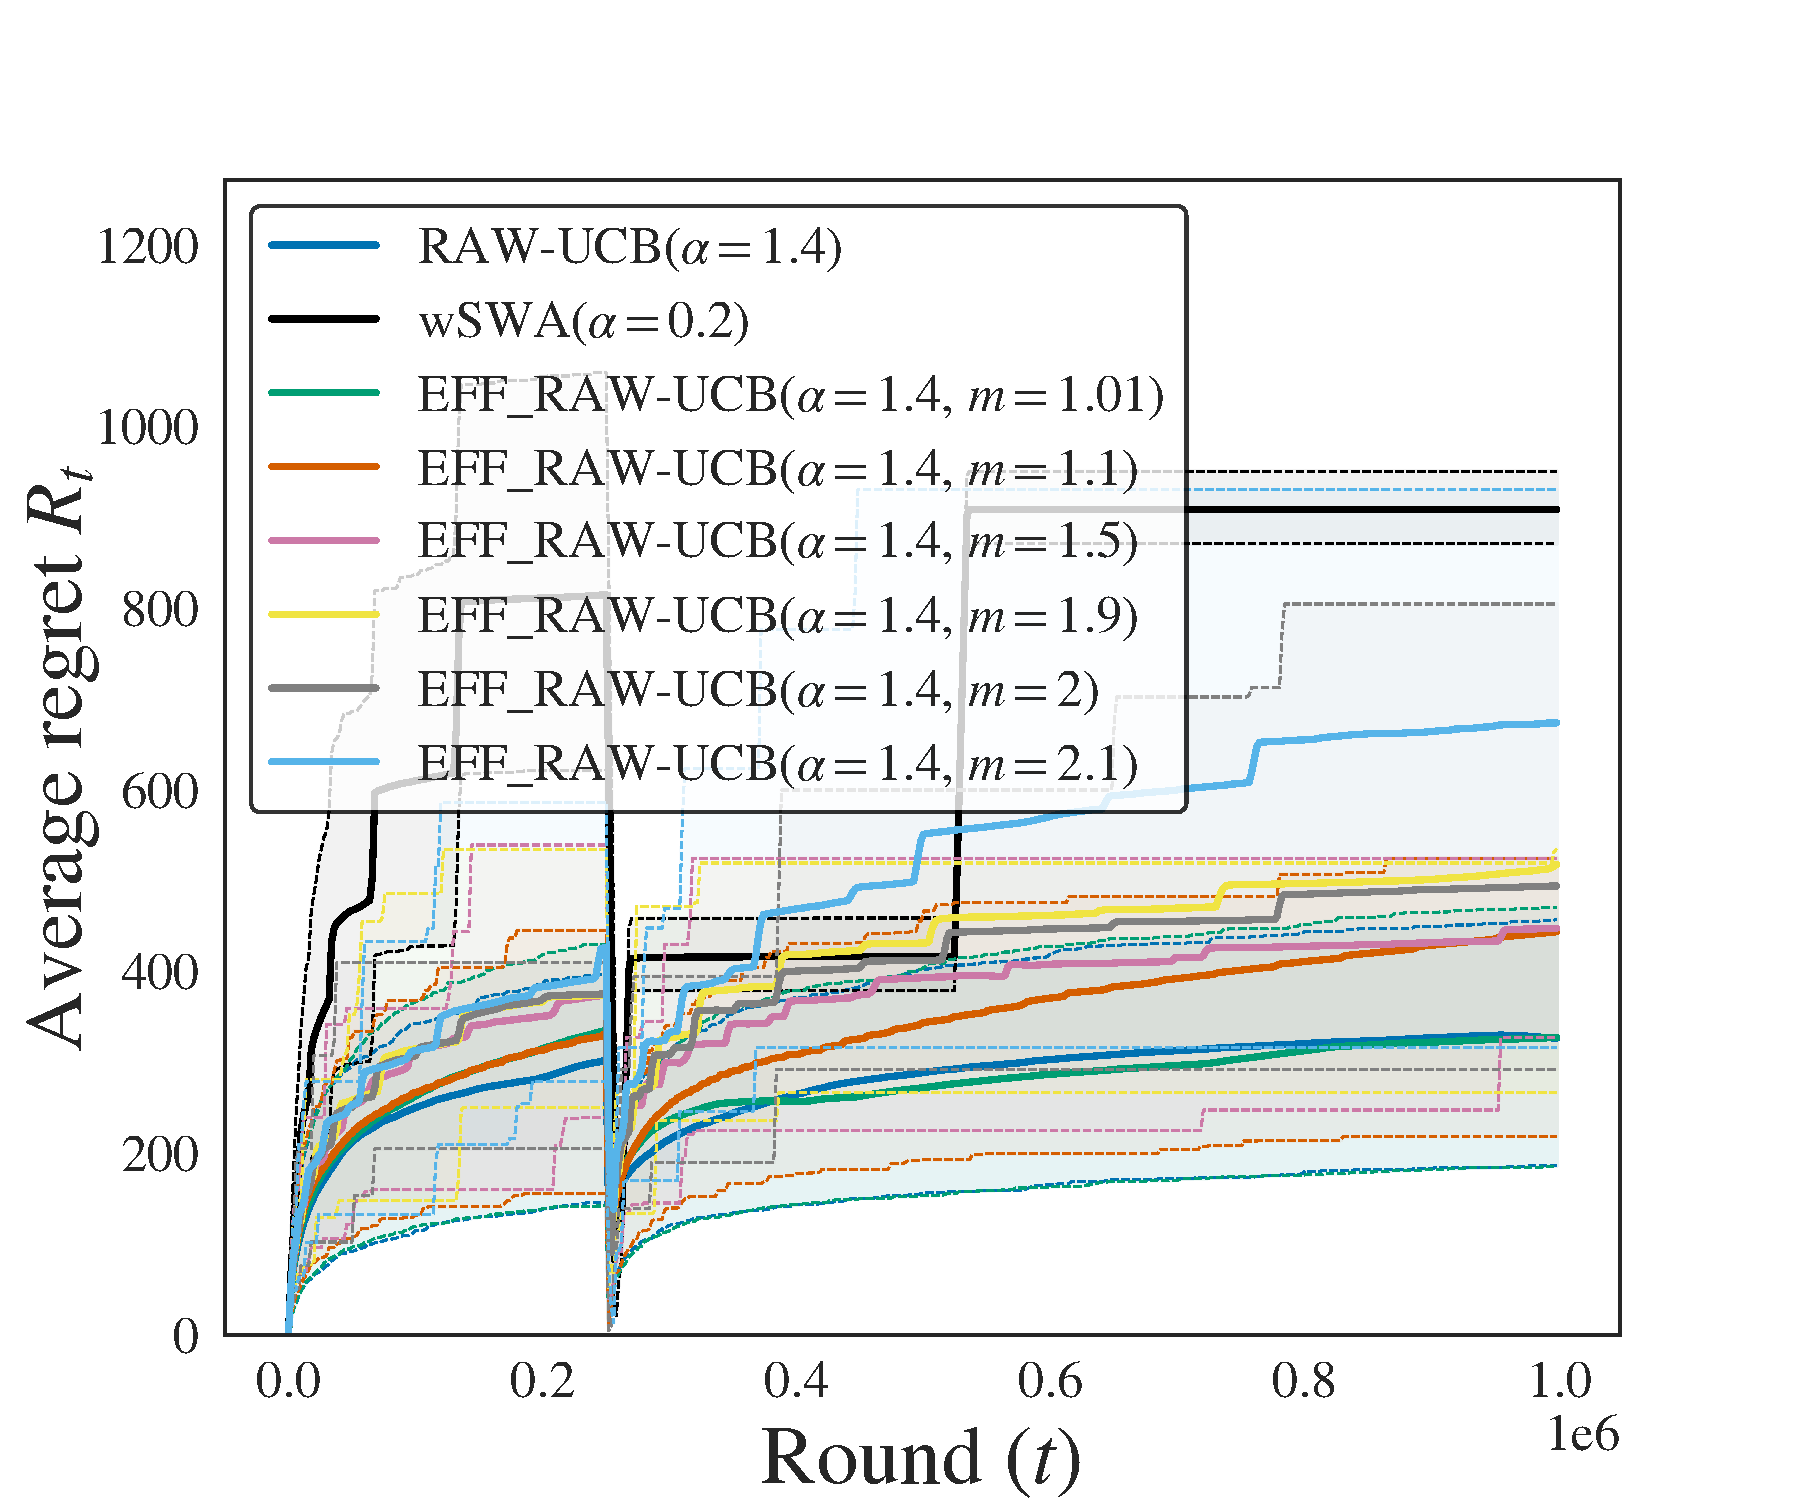
\includegraphics[width = 0.8\textwidth]{2.1Rested/fig/fig_eff.pdf}
\caption{Regret across time. Average over 1000 runs. We highlight the $\left[10\%, 90\%\right]$ confidence region.} 
\label{fig:rested-eff}
\end{figure*}

\begin{table}[ht!]
\centering
\begin{tabular}{|c|c|c|}
\hline
\textbf{Policy} &\textbf{Running time (s)} & \textbf{comparison w/ \RAWUCB}\\ \hline
\RAWUCB ($\alpha = 1.4$) & 38837      & 100$\%$                \\ \hline
\EFFRAW($\alpha = 1.4$, $m=1.01$)    & 169       & 0.4 $\%$             \\ 
\EFFRAW($\alpha = 1.4$, $m=1.1$)    & 121    & 0.3 $\%$                   \\ 
\EFFRAW($\alpha = 1.4$, $m=1.5$)    & 115    & 0.3 $\%$                  \\ 
\EFFRAW($\alpha = 1.4$, $m=1.9$)    & 112       & 0.3 $\%$               \\ 
\EFFRAW($\alpha = 1.4$, $m=2$)    & 119       & 0.3 $\%$               \\ 
\EFFRAW($\alpha = 1.4$, $m=2.1$)    &  114      & 0.3 $\%$               \\ \hline
\wSWA($\alpha = 0.002$)   & 41   & 0.1 $\%$                     \\ 
\wSWA($\alpha = 0.02$)    & 43  & 0.1 $\%$                      \\ 
\wSWA($\alpha = 0.2$)    & 49    & 0.1 $\%$                    \\ \hline
\end{tabular}
  \caption{Average running time and comparison with {\RAWUCB} for the efficient benchmark.}
  \label{tab:time-figeff}
\end{table}

\paragraph{Results.} Overall, the regret performance of \EFFRAW is up to $50\%$ worse than the performance of \RAWUCB. The worst versions correspond to larger values of $m$. Yet, there are few counter-examples: $m=2$ performs similarly to $m=1.9$ and $m=1.1$ performs similarly than $m=1.5$ at the end of the game. We remark that there are discontinuities in the regret of the efficient algorithms. It is because the statistics are not updated at every round. Hence, when one statistic is updated, it can change the behavior of the algorithm for many rounds. 

In terms of running time, the efficient trick drastically reduces the running time of \EFFRAW. While the theory suggests that there is no free lunch, we remark that setting a value very close to $1$ does reduce the running time and recover very similar regret performance. Surprisingly, the running time are quite similar for $m \in \bra{1.1, 2.1}$. The running time when $m=1.01$ is only 48 seconds (+ 40$\%$) larger than for $m=1.1$ while there are 10 times more confidence intervals to compute. Hence, we believe that the UCBs computation time for $m \in \bra{1.1, 2.1}$ is quite small compared to other fixed costs in the implementation (the reward generation, the $\log\pa{t}$ computation, etc.).   However, \wSWA is still faster than \EFFRAW. It is surprising because its complexity is $\cO\pa{T^{\nicefrac{2}{3}}}$, which is much larger than \EFFRAW 's $\cO\pa{K\log_m{T}}$. Yet, in practice, \wSWA computes $T^{\nicefrac{2}{3}}$ sums while \EFFRAW computes $\cO\pa{K\log_m{T}}$ ucb indexes (with a $\sqrt{\cdot}$ and a $\log$ function).

We believe that we could speed up \EFFRAW with low-level implementation tricks. For instance, the profiling of the code indicates that the $\log$ function is very expensive. One could compute faster the $\log(t+1)$ from the previous value $\log(t)$. Yet, these low-level implementation tricks are not in the scope of this thesis. 

\subsubsection{Simulated benchmark $\#$1 (2 arms) and $\#$2 (10 arms).}
\paragraph{Setup and Algorithms.} We study the two benchmarks described in Subsection~\ref{subsec:rested-experiment1} and Section~\ref{sec:rested-experiment}. In Figures~\ref{fig:rested-eff1} and~\ref{fig:rested-eff2}, we compare \RAWUCB with \EFFRAW for two values of m $\ev{1.1, 2}$.

\paragraph{Results.} For the two values, we remark that \EFFRAW have a slightly worse performance than \RAWUCB (up to $50\%$ for $m=2$). It confirms our theoretical analysis which suggests that the performance of \EFFRAW is only at a constant factor of the performance of \RAWUCB. It also confirms that the smaller the $m$, the less regret we suffer. 
\begin{figure*}[!ht]
\centering
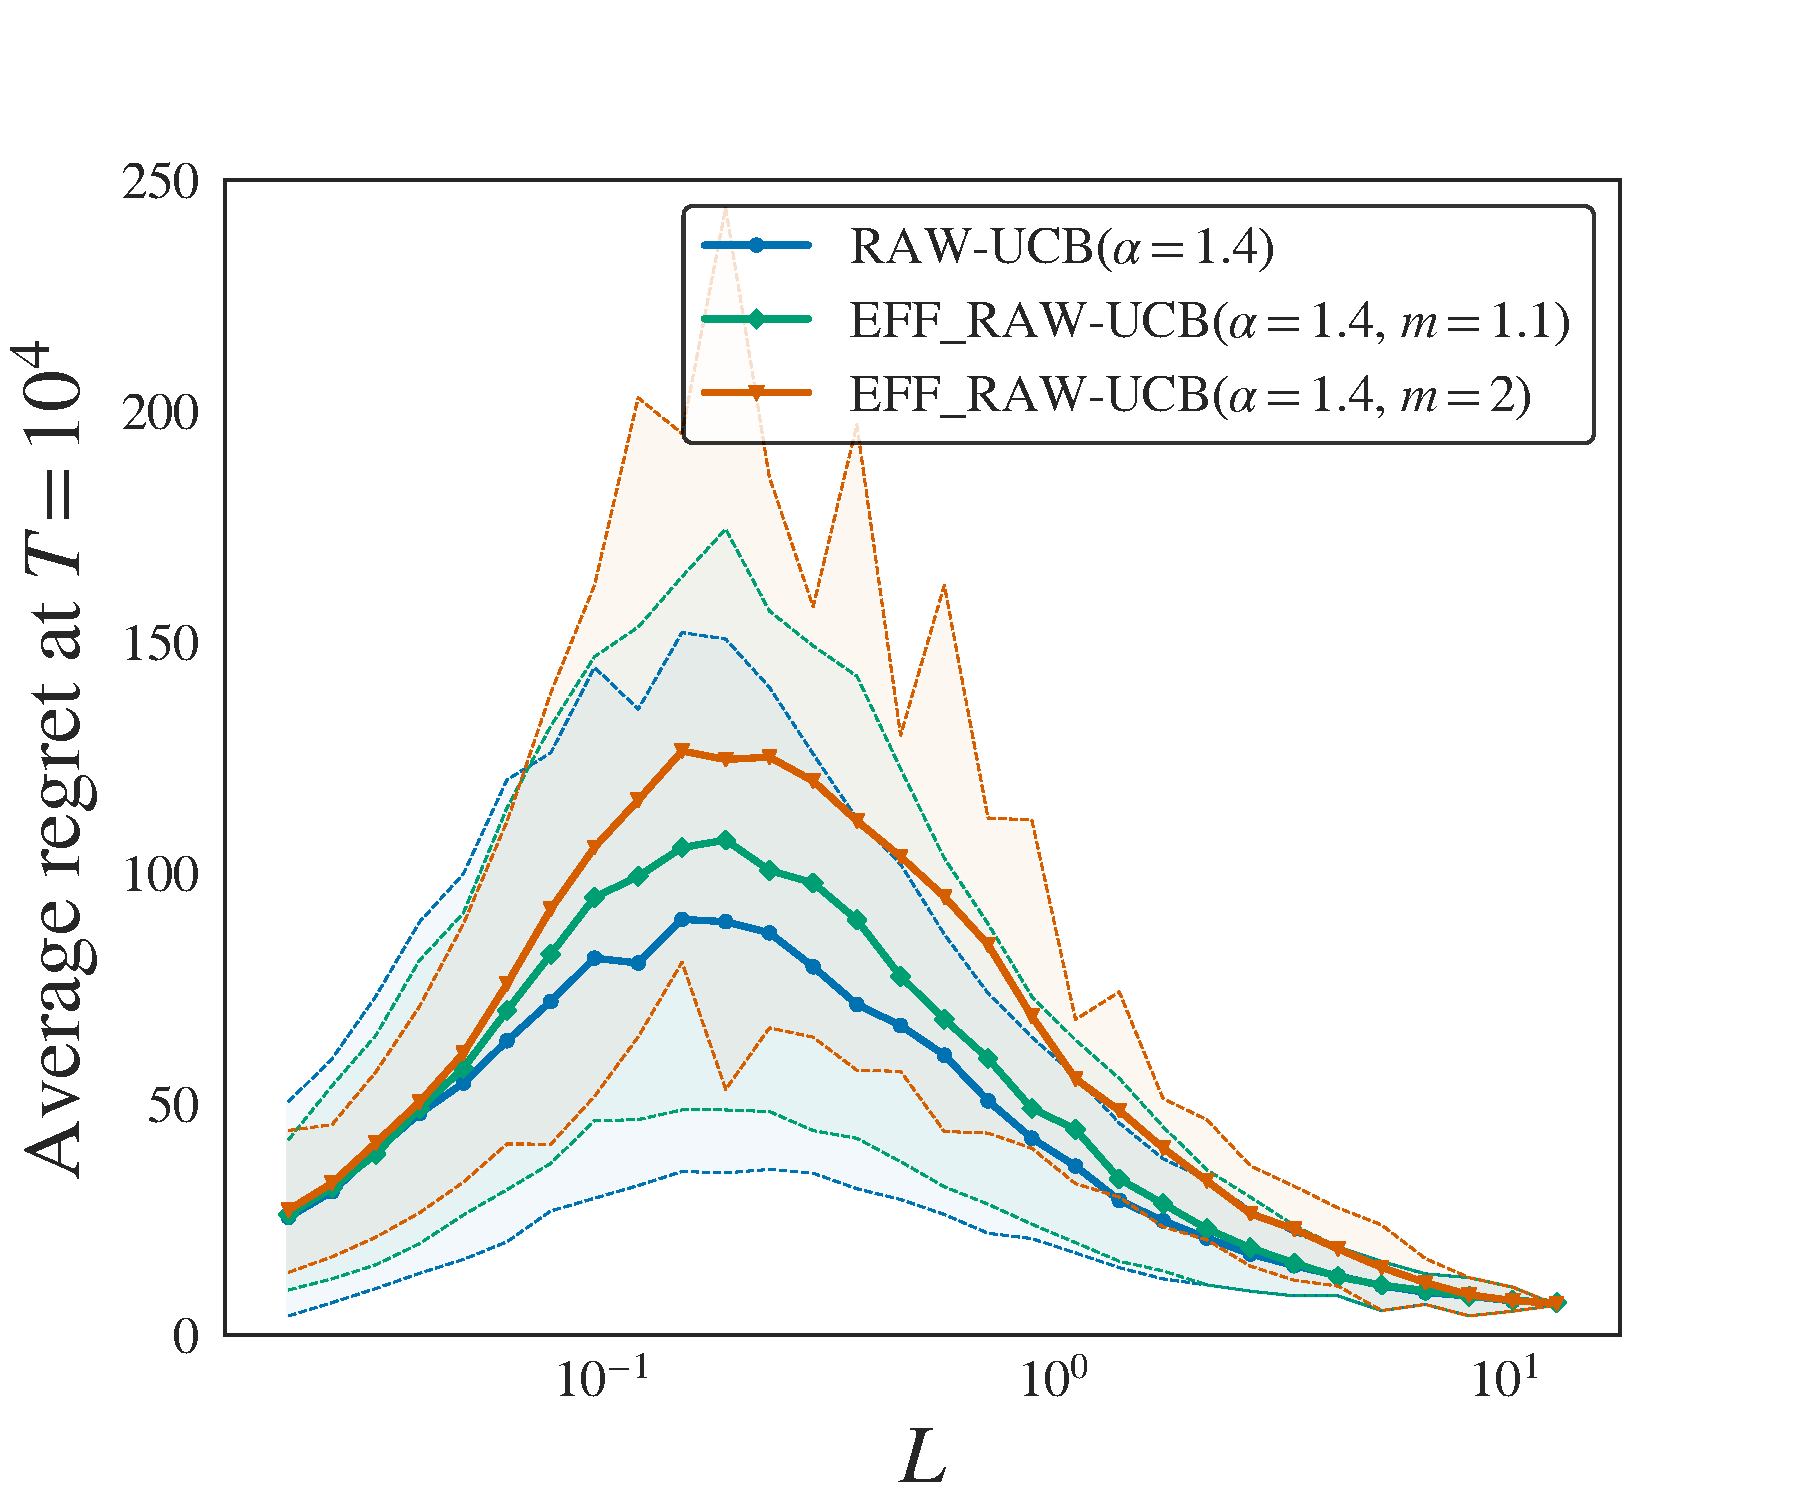
\includegraphics[clip, width= 0.51\textwidth]{2.1Rested/fig/fig1A_eff.pdf}
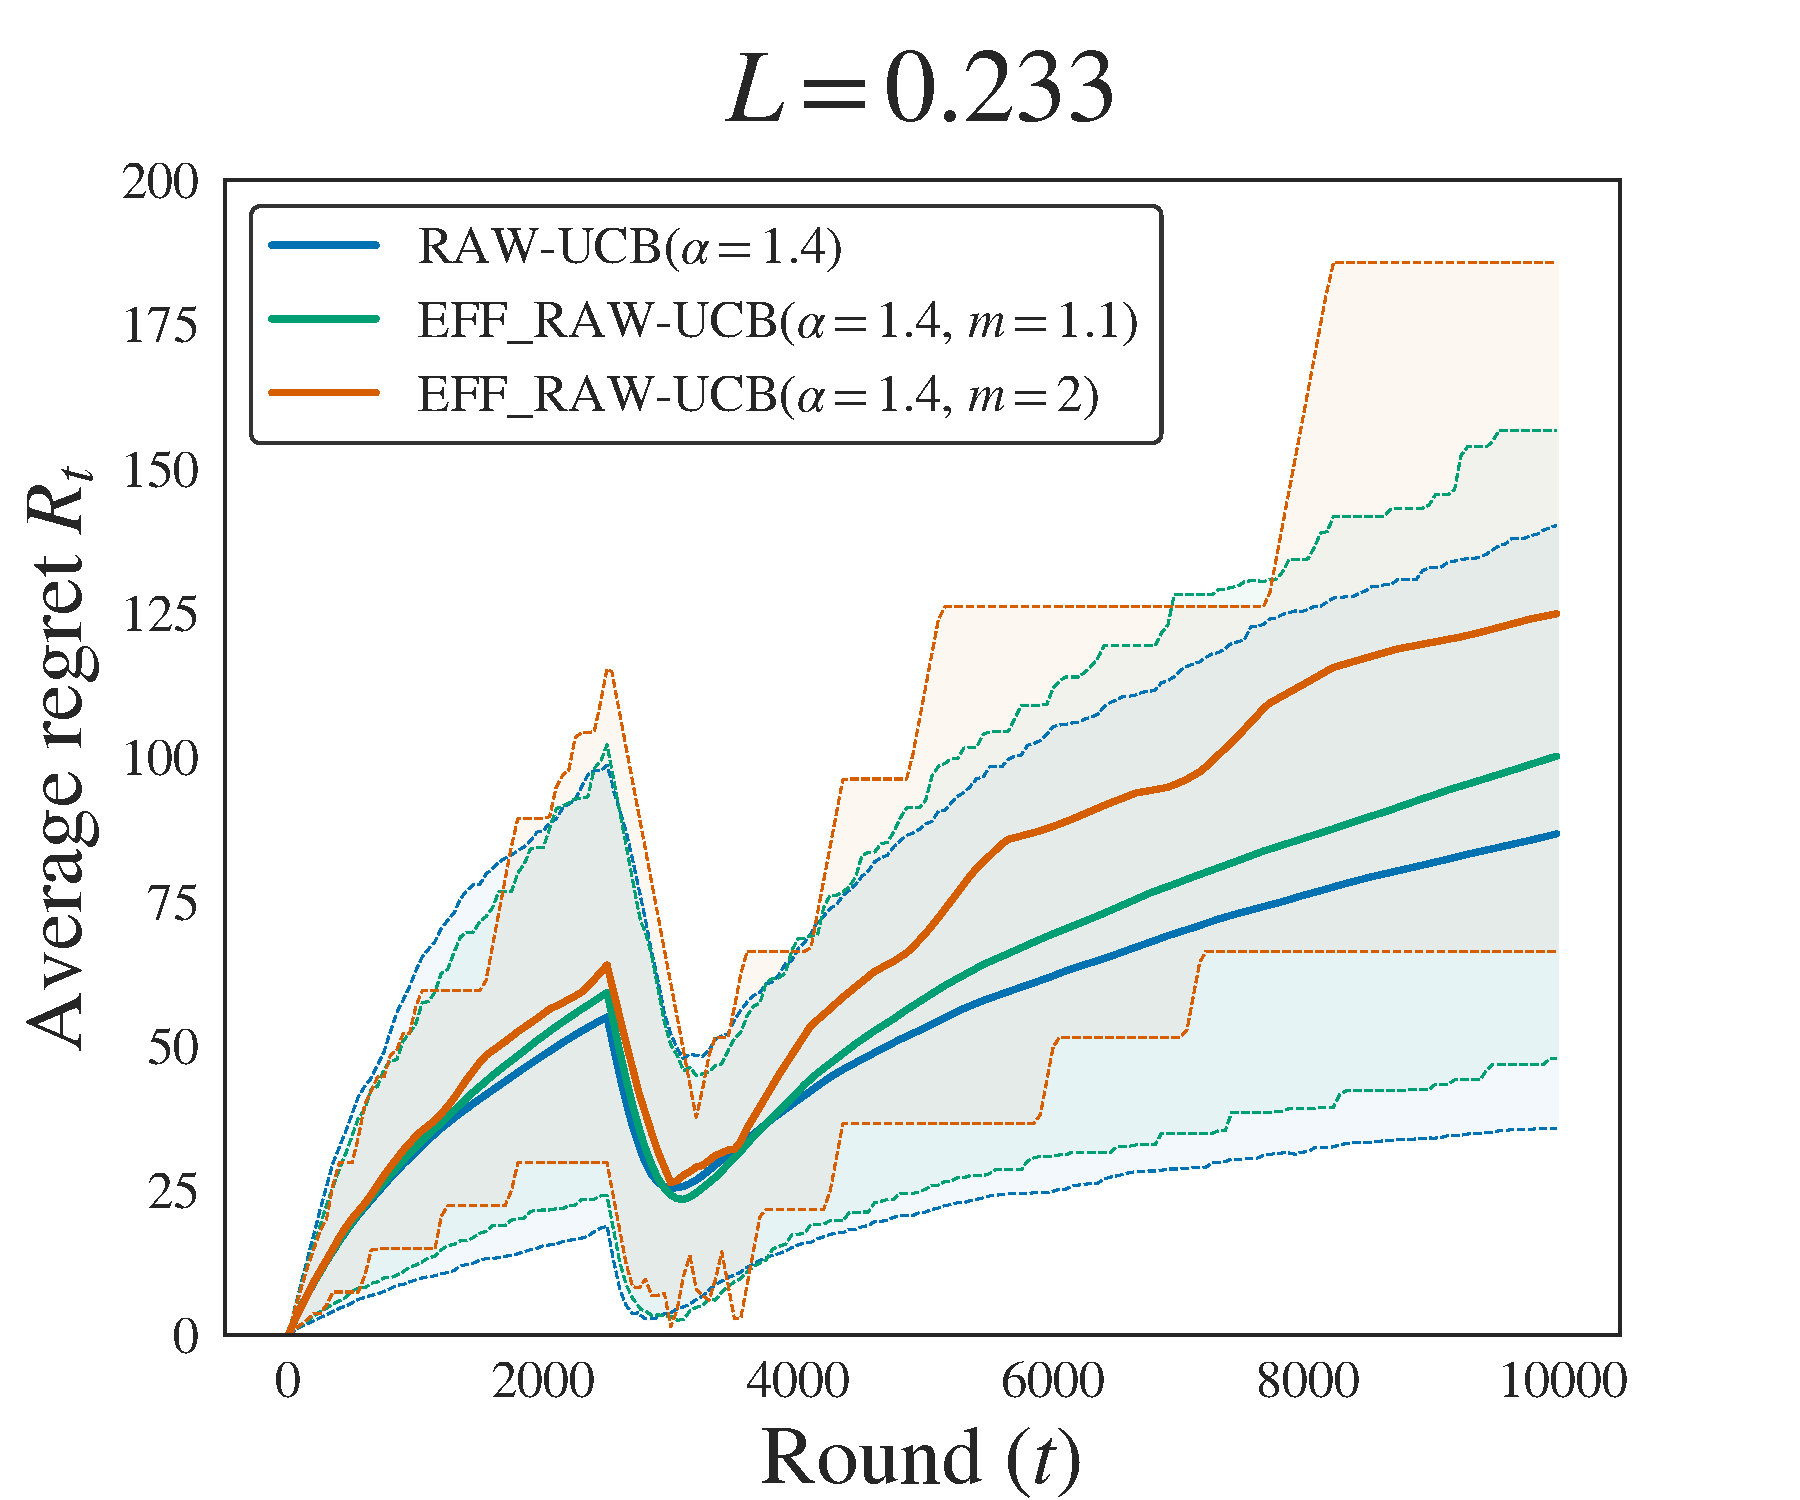
\includegraphics[clip, width= 0.49\textwidth]{2.1Rested/fig/fig1B_eff.pdf}
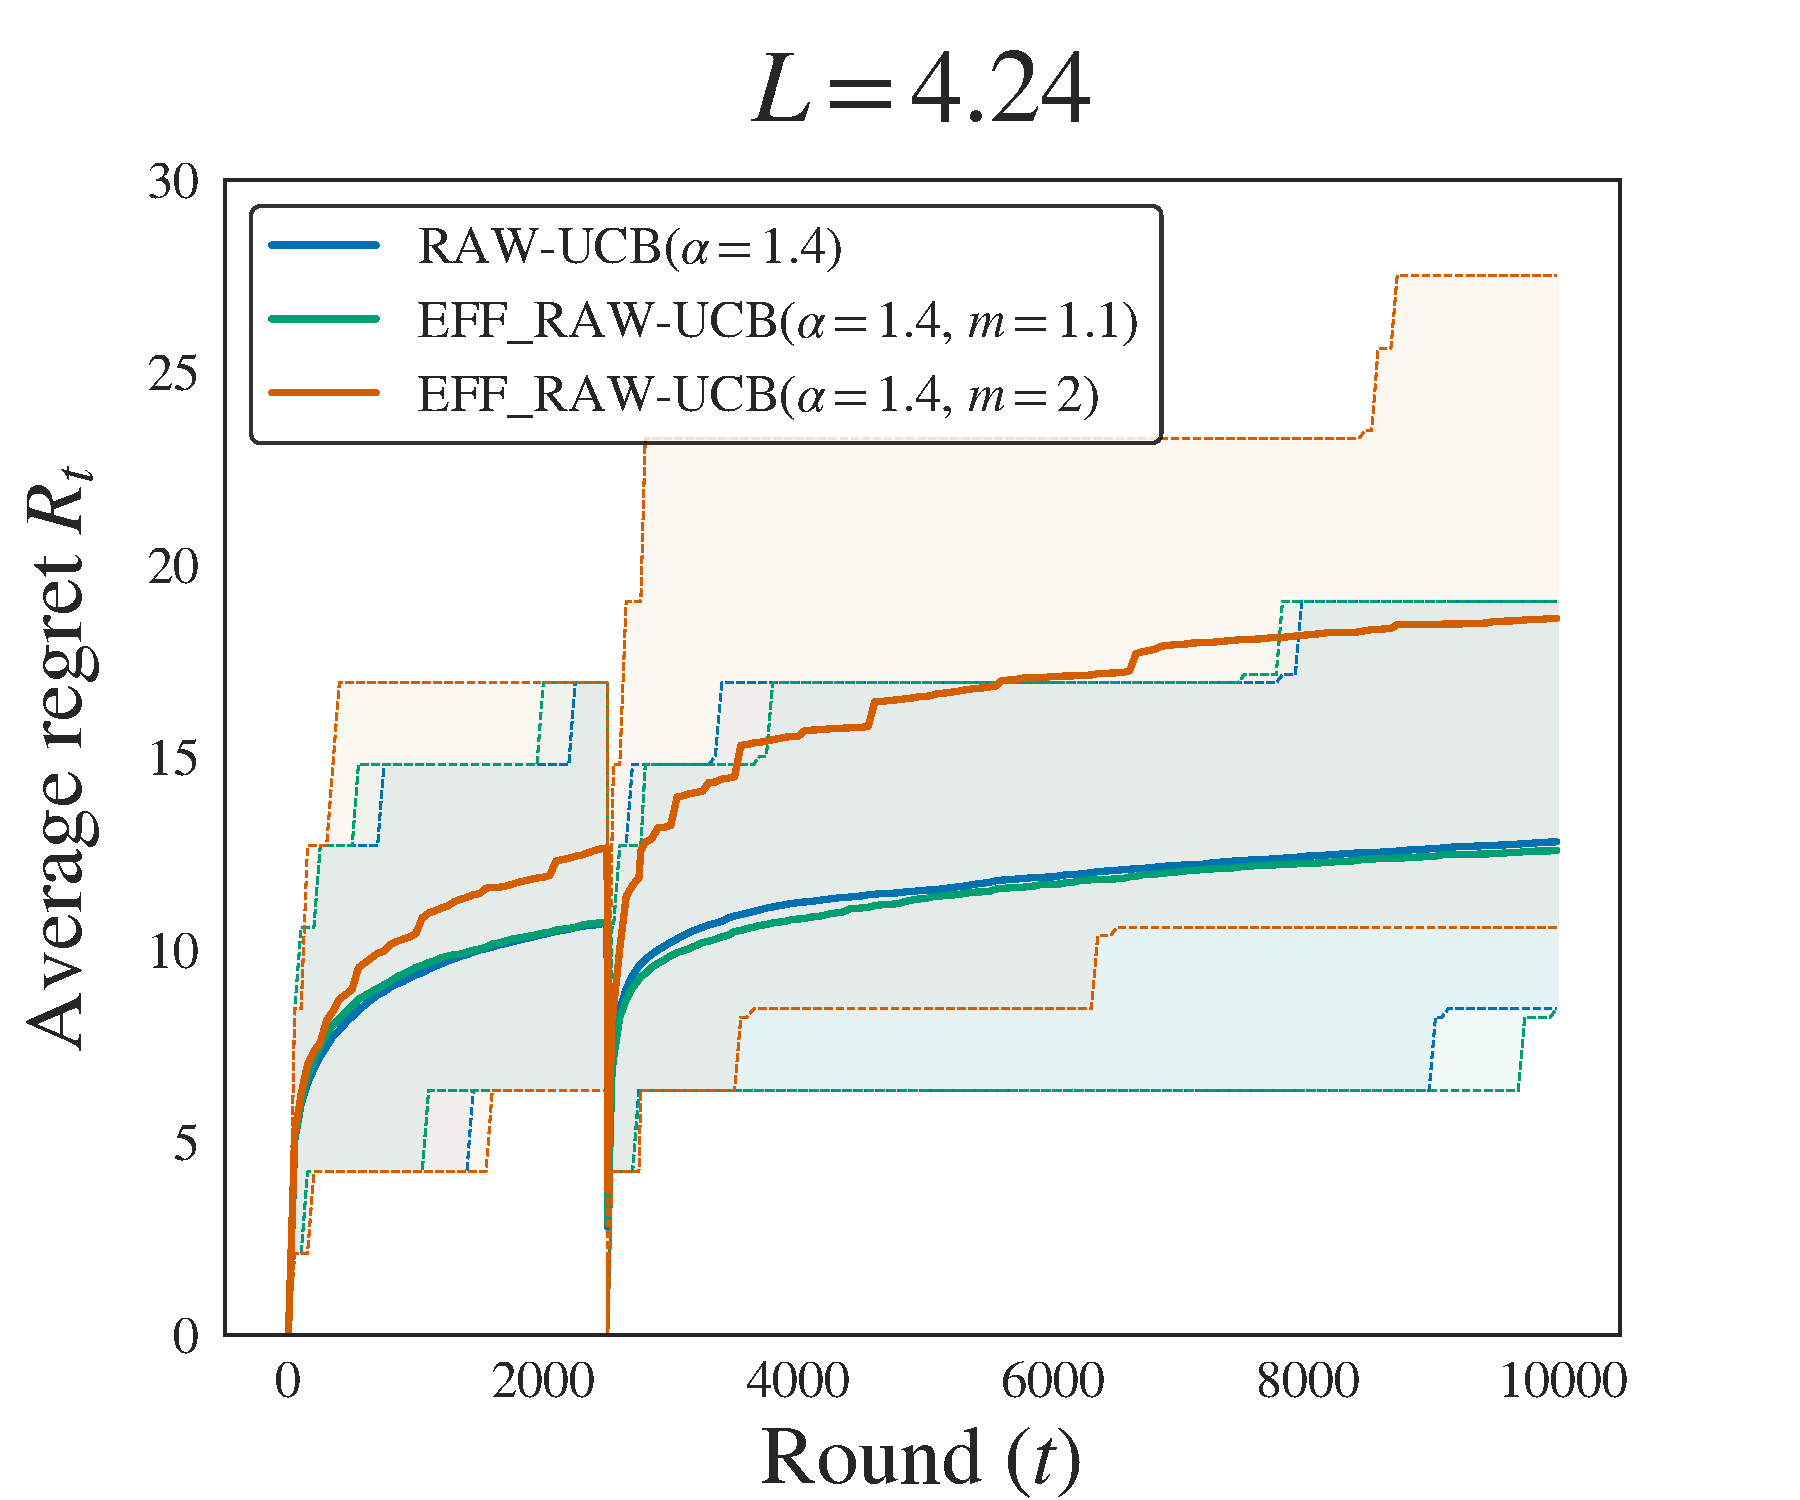
\includegraphics[clip, width= 0.49\textwidth]{2.1Rested/fig/fig1C_eff.pdf}
\caption{\textbf{Top:} Regret at the end of the game for different values of $L$. \textbf{Bottom:} Regret across time for two values of $L$. Average over 1000 runs. We highlight the $\left[10\%, 90\%\right]$ confidence region.}
\label{fig:rested-eff1}
\end{figure*}


\begin{figure*}[!ht]
\centering
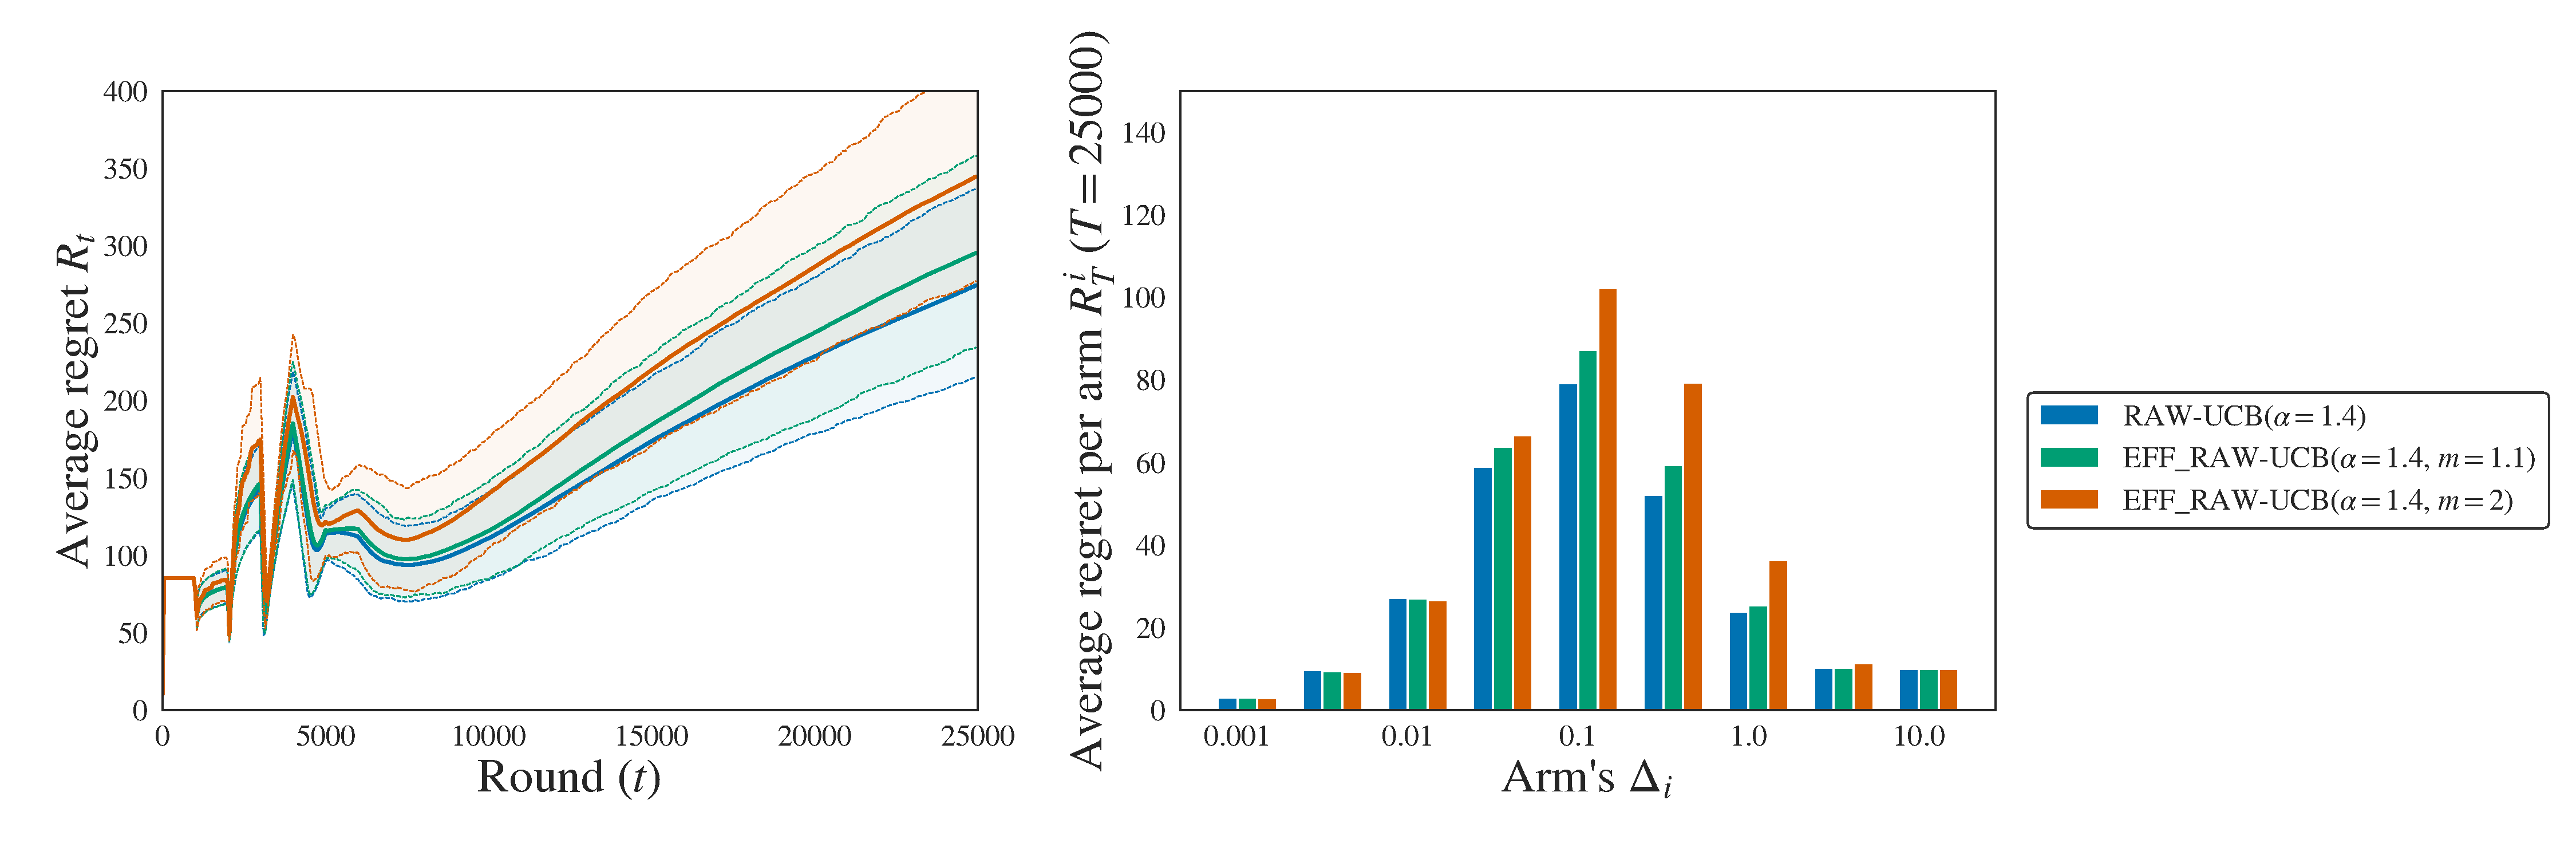
\includegraphics[width = 0.99 \textwidth]{2.1Rested/fig/fig2_eff.pdf}
\caption{\textbf{Left:} Regret at the end of the game for different values of $L$. \textbf{Middle, Right:} Regret across time for two values of $L$. Average over 1000 runs. We highlight the $\left[10\%, 90\%\right]$ confidence region.}
\label{fig:rested-eff2}
\end{figure*}

Notice that the two algorithms run in 3 seconds in average\footnote{3.0 s for $m=2$, 3.3 s for $m=1.1$} versus 25 seconds for \RAWUCB and 1 second for \wSWA. It shows that \EFFRAW effectively reduces the computation cost of \RAWUCB, even for a shorter horizon.



\subsection{Conclusion}
In this section, we provide a new update scheme which keeps $\cO\pa{\log_m t}$ averages with geometrical windows sequence of parameter $m$. These averages are updated with a delay which is proportional to the window size times $\nicefrac{m-1}{m}$. We show that when we plug this efficient update scheme in our algorithms, we recover the same upper bounds as the original algorithms with a larger multiplicative constant. However, the computational complexity is considerably reduced from $\cO(T)$ to $\cO(K\log_m T)$. We also show that in practice we can recover almost the same performance as the classical algorithms but with a computational cost that is comparable with $\wSWA$.
%!TEX root = ../main.tex 
\section{How harder are rotting bandits ?}
\label{sec:howhard}
In the last sections, we presented \RAWUCB, an algorithm which extends the results of \UCBone \citep{auer2002finite} on stationary bandits to the more general rotting bandits setup. Hence, we conclude that rotting bandits are not much harder than stationary ones. 

Yet, \UCBone is only near asymptotic and minimax optimal. In Section~\ref{sec:stoch-bandits}, we explain that a better tuning of the confidence levels allows \UCB variant to match the asymptotic and minimax rates for gaussian bandits.

This section investigates the impact of confidence levels tuning on \RAWUCB. How does it compare with \UCB on stationary bandits?  Does it improve the performance of \RAWUCB on our rotting benchmarks? 

\subsection{{\RAWUCBpp}}
We introduce \RAWUCBpp, an algorithm which uses the \RAWUCB procedure (Alg.\ref{alg:RAWUCB}) with a new index,
\begin{multline}
\label{eq:rawpp_index}
\operatorname{ind}(i,t, \delta_{t,h}) \triangleq \min_{h\leq N_{i,t-1}}\pa{ {\hmu}_i^h(\Nitmone) + \sqrt{\frac{2\sigma^2\log_+\pa{\nicefrac{2}{\delta_{t,h}}}}{h}}}\\ \text{ with } \; \delta_{t,h} \triangleq \frac{2\pa{\nicefrac{Kh}{t}}^\alpha}{\pa{1+ \log_+\pa{\nicefrac{t}{Kh}}}^\beta}\CommaBin
\end{multline}

with $\log_+\pa{\cdot} \triangleq \max\pa{\log\pa{\cdot}, 0}$. The main difference with the index of \RAWUCB in Equation~\ref{eq:raw_index} is the more complex confidence level. First, we multiply our confidence level by $Kh$ and replace $\log$ by $\log_+$. This is similar to the $\delta = \nicefrac{KN_{i,t}}{t}$ of \MOSSa  \citep{degenne2016anytime}. We replace $N_{i,t}$ - the number of pulls of arm $i$ at the round $t$- by $h$, the number of sample in the associated average. Indeed, let us consider a two-arm bandit problem where the first arm has a much larger value $\mu_2 + 100 \sigma$ than the second one (with value $\mu_2$) at the beginning of the game. Hence, at the beginning of the game, $N_{1,t} \sim t$ because \RAWUCBpp can quickly identify arm $1$ as the current best arm. After $\frac{T}{2}$ pulls, arm $1$ abruptly decay to a value $\mu_2 + \sigma$. If we do not replace $N_{i,t}$ by $h$ in the confidence levels in Equation~\ref{eq:rawpp_index}, the exploration bonus would be canceled until the end of the game for all the UCB of arm $1$ because $\frac{KN_{i,t}}{t} > 1$. Without the exploration bonus, there is a large enough probability that the index of arm $1$ takes a value below $\mu_2$. Indeed, since we take the minimum across indexes, if the first reward sample after the decay is below $\mu_2$, then the meta-index will be below $\mu_2$. In this case, \RAWUCB may pull arm $2$ until the end of the game and suffer at least $\cO\pa{\sigma T}$ regret. Replacing $N_{i,t}$ by $h$ restore the exploration bonus for arms which have recently decay. 

Second, we add a logarithmic exploration inflation factor. Notice that we also divide $t$ by $Kh$ in the inner logarithm, as it is done for \KLUCBpp \citep{menard2017klucb++}. When the noise is not gaussian, the concentration results are slightly less tight and the asymptotic optimality proof often needs this factor. For instance, \citet{cappe2013klucb} use a factor $\log\pa{t}^{-3}$ in their theory, but they recommend to not use it in practice. However, for \RAWUCB, we believe that extra-exploration is needed in practice. Indeed, we find our best experimental performance for $\alpha=1.4$ which is larger than the asymptotic optimal tuning for \UCB $\alpha=1$ \citep{lattimore2020banditbook}. In our theory in Section~\ref{sec:theory}, we increase $\alpha$ by one compared to \UCBone to ensure that the $t$ (instead of $K$) constructed statistics were into the confidence levels. 




\subsection{Experiments}
\subsubsection{Stationary Experiment}

\paragraph{Setup.} We consider a stationary bandits with two arms with $\mu_1= 0$ and $\mu_2 = \Delta$. We consider two different values of $\Delta \in \left\{0.01, 1\right\}$. The rewards are then generated by applying a Gaussian i.i.d.\,noise $\mathcal{N}\left(0,\subgaussian = 1\right)$. We run the experiment with the horizon $T=10^6$.

\paragraph{Algorithms.} We consider \UCB and \MOSSa \citep{degenne2016anytime}. We tune \UCB with asymptotic optimal confidence level $\sqrt{\nicefrac{2\log\pa{t}}{\Nit}}$ \citep{lattimore2020banditbook}. For \MOSSa, we use $\sqrt{\nicefrac{2\log\pa{\nicefrac{t}{K\Nit}}}{\Nit}}$, which corresponds to a tuning of its parameter $\alpha = 3$. We test \RAWUCBpp with many different values, but we display two different sets of values $\alpha = 1$ and $\beta = 3.5$ or $\alpha = 2$ and $\beta=0$. These two sets of values give the most consistent performance on the two problems. We add \RAWUCB with $\alpha = 1.4$ for comparison. For \RAWUCB and \RAWUCBpp , we use the efficient version with $m=1.01$ which performs similarly than the classical algorithm Subsection~\ref{ss:eff-exp}.

\begin{figure*}[ht]
\centering
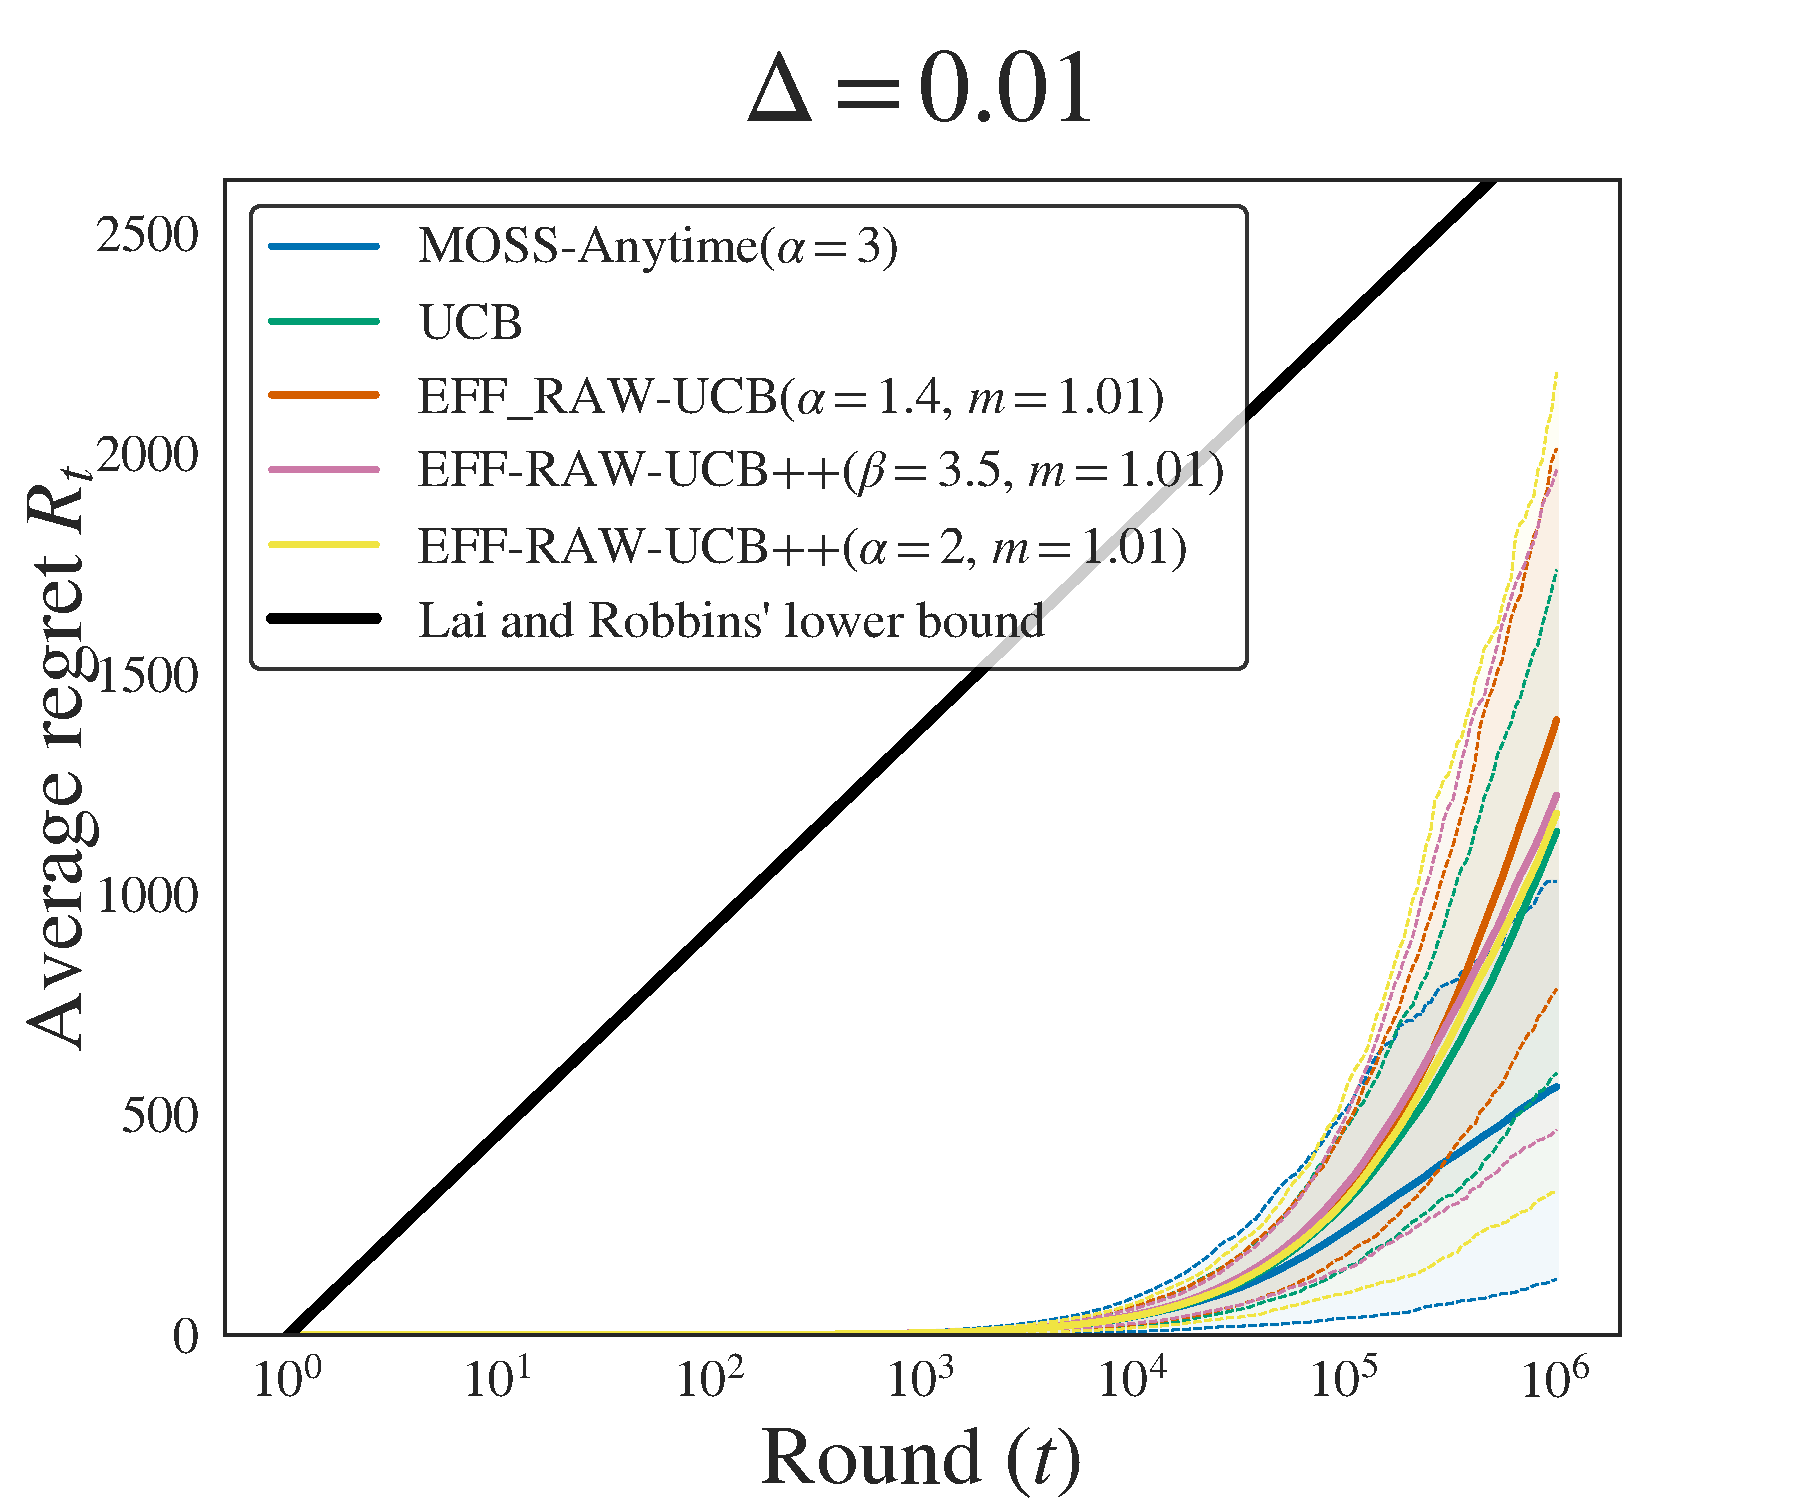
\includegraphics[clip, width= 0.49\textwidth]{2.1Rested/fig/fig_asy0,01.pdf}
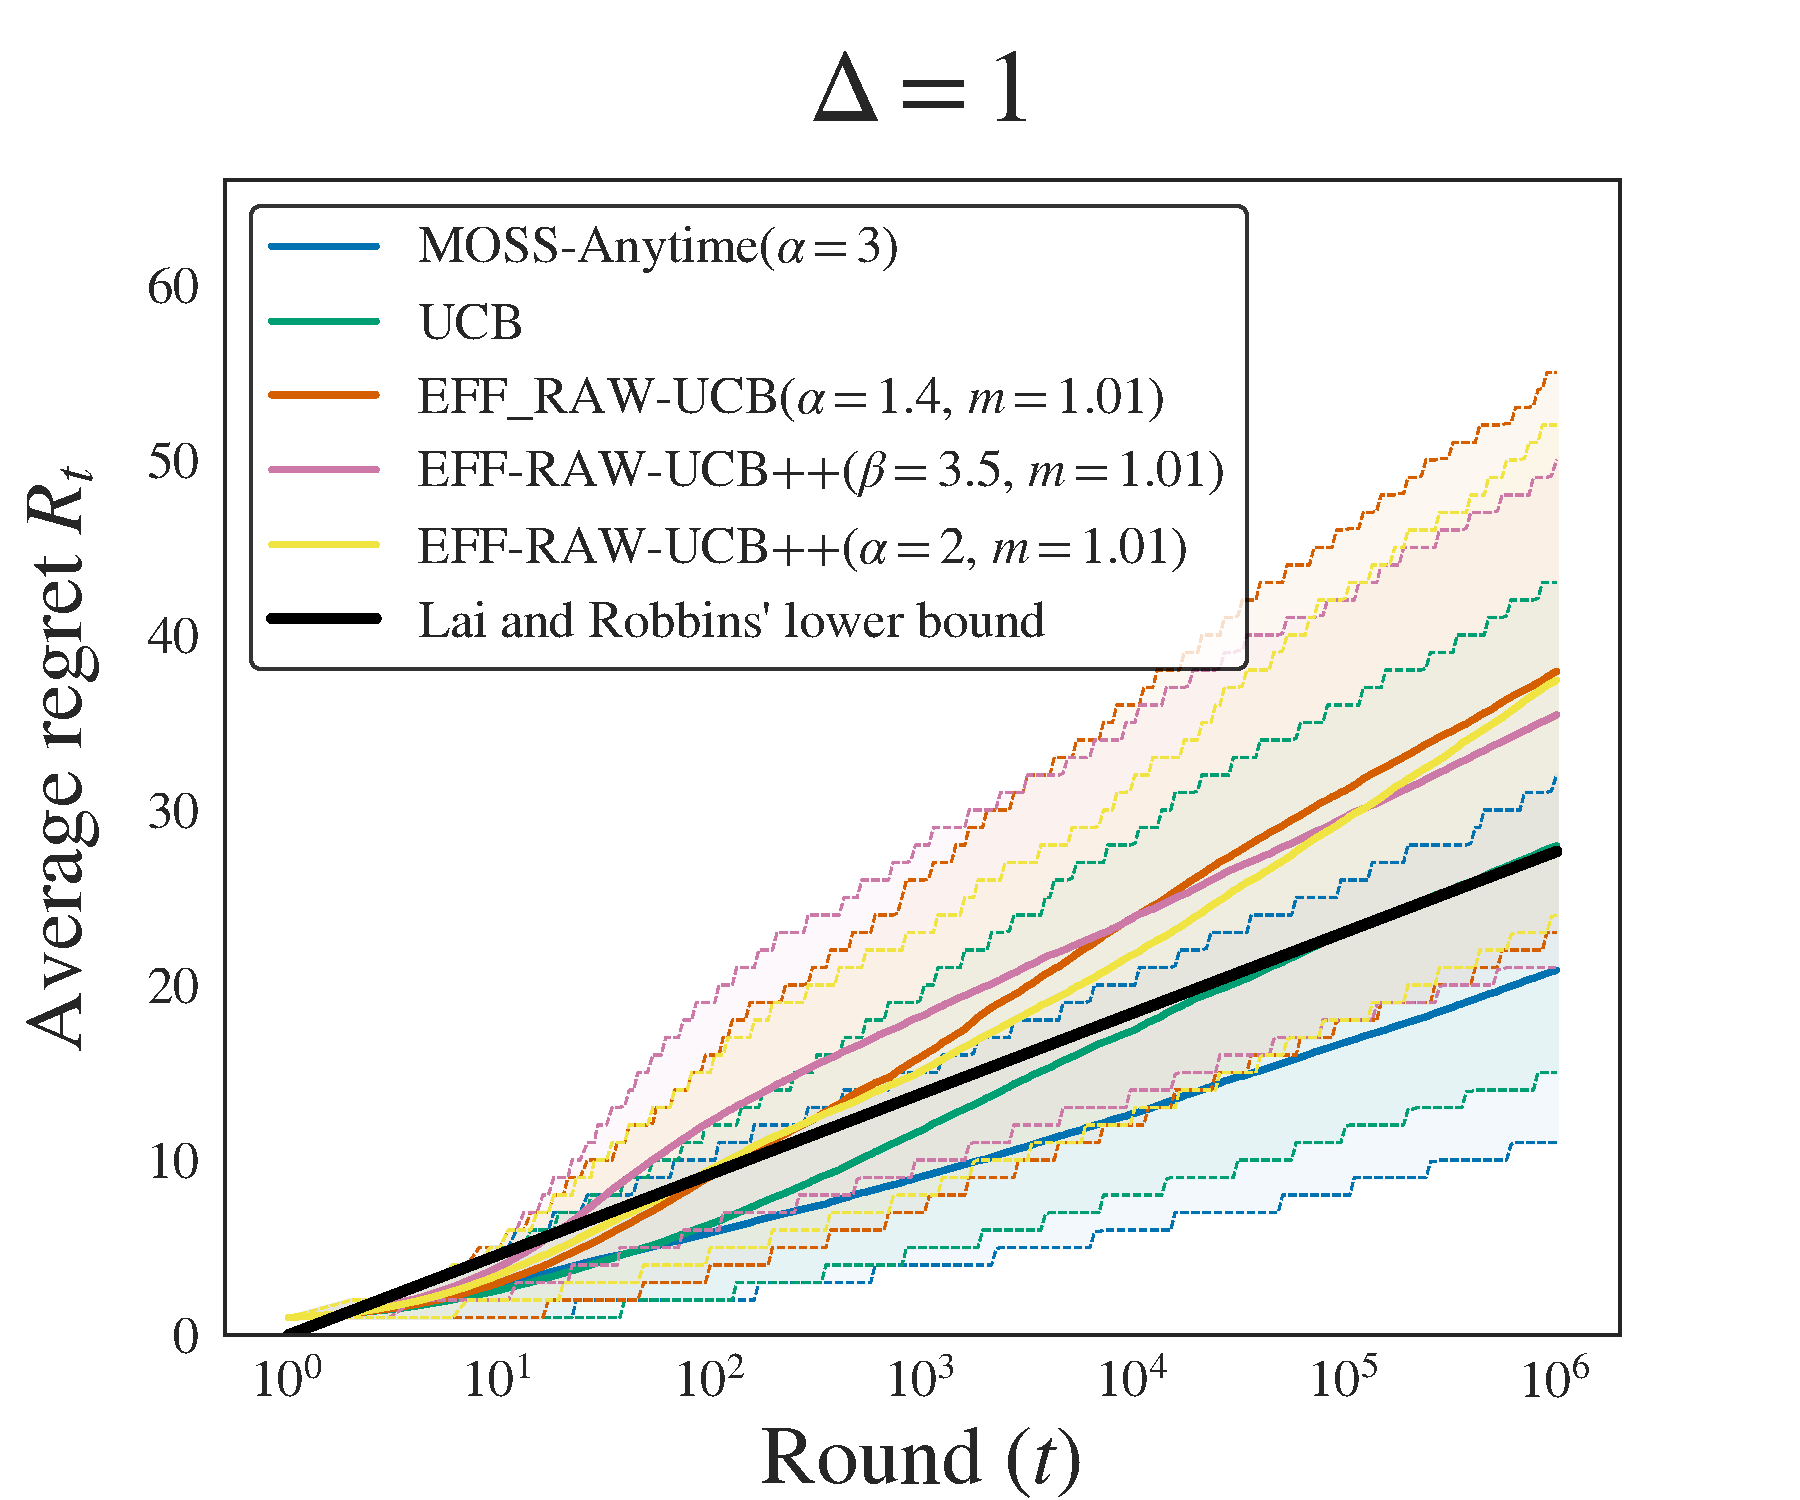
\includegraphics[clip, width= 0.49\textwidth]{2.1Rested/fig/fig_asy1.pdf}
\caption{Stationary experiments}
\label{fig:stationary-experiment}
\end{figure*}
\paragraph{Results.}  \RAWUCBpp seems to improve slightly the results compare to \RAWUCB. Yet, the improvement is not as significant than between \MOSSa and \UCB. On the $\Delta=1$ experiment, we see that the tuning with the logarithm ($\beta=3.5$) seems to enjoy better asymptotic guarantee than the tuning with $\alpha = 2$. Yet, it is not clear if \RAWUCBpp ($\beta=3.5$) is asymptotic optimal with respect to the Lai and Robbin's lower bound. However, at finite horizon, the different parameters are quite close to each other.



\subsubsection{Rotting Experiments $\#$1 (2 arms) and $\#$2 (10 arms).}
\paragraph{Setup and Algorithms.} We study the two benchmarks described in Subsection~\ref{subsec:rested-experiment1} and Section~\ref{sec:rested-experiment}. In Figures~\ref{fig:rested-eff1} and~\ref{fig:rested-eff2}, we compare \EFFRAWpp ($\alpha=2$, $m=1.01$) with \EFFRAW  ($\alpha=1.4$, $m=1.01$). The parameters $\alpha$ were selected according to previous experiments.

\paragraph{Results.} \EFFRAWpp performs slightly better than \EFFRAW for almost any experiments and at almost any rounds. A noticeable exception is when $L$ is large in the two-arms experiment: the result of \EFFRAWpp is slightly worse than for \EFFRAW. Overall, the results suggest that the aggressive confidence tuning technique of stationary bandits also improves the rotting adaptivity. Yet, we notice that the confidence levels with $\alpha =2$ are less tight than the tuning of \MOSSa (which would correspond to $\alpha=1$).

\begin{figure*}[ht]
\centering
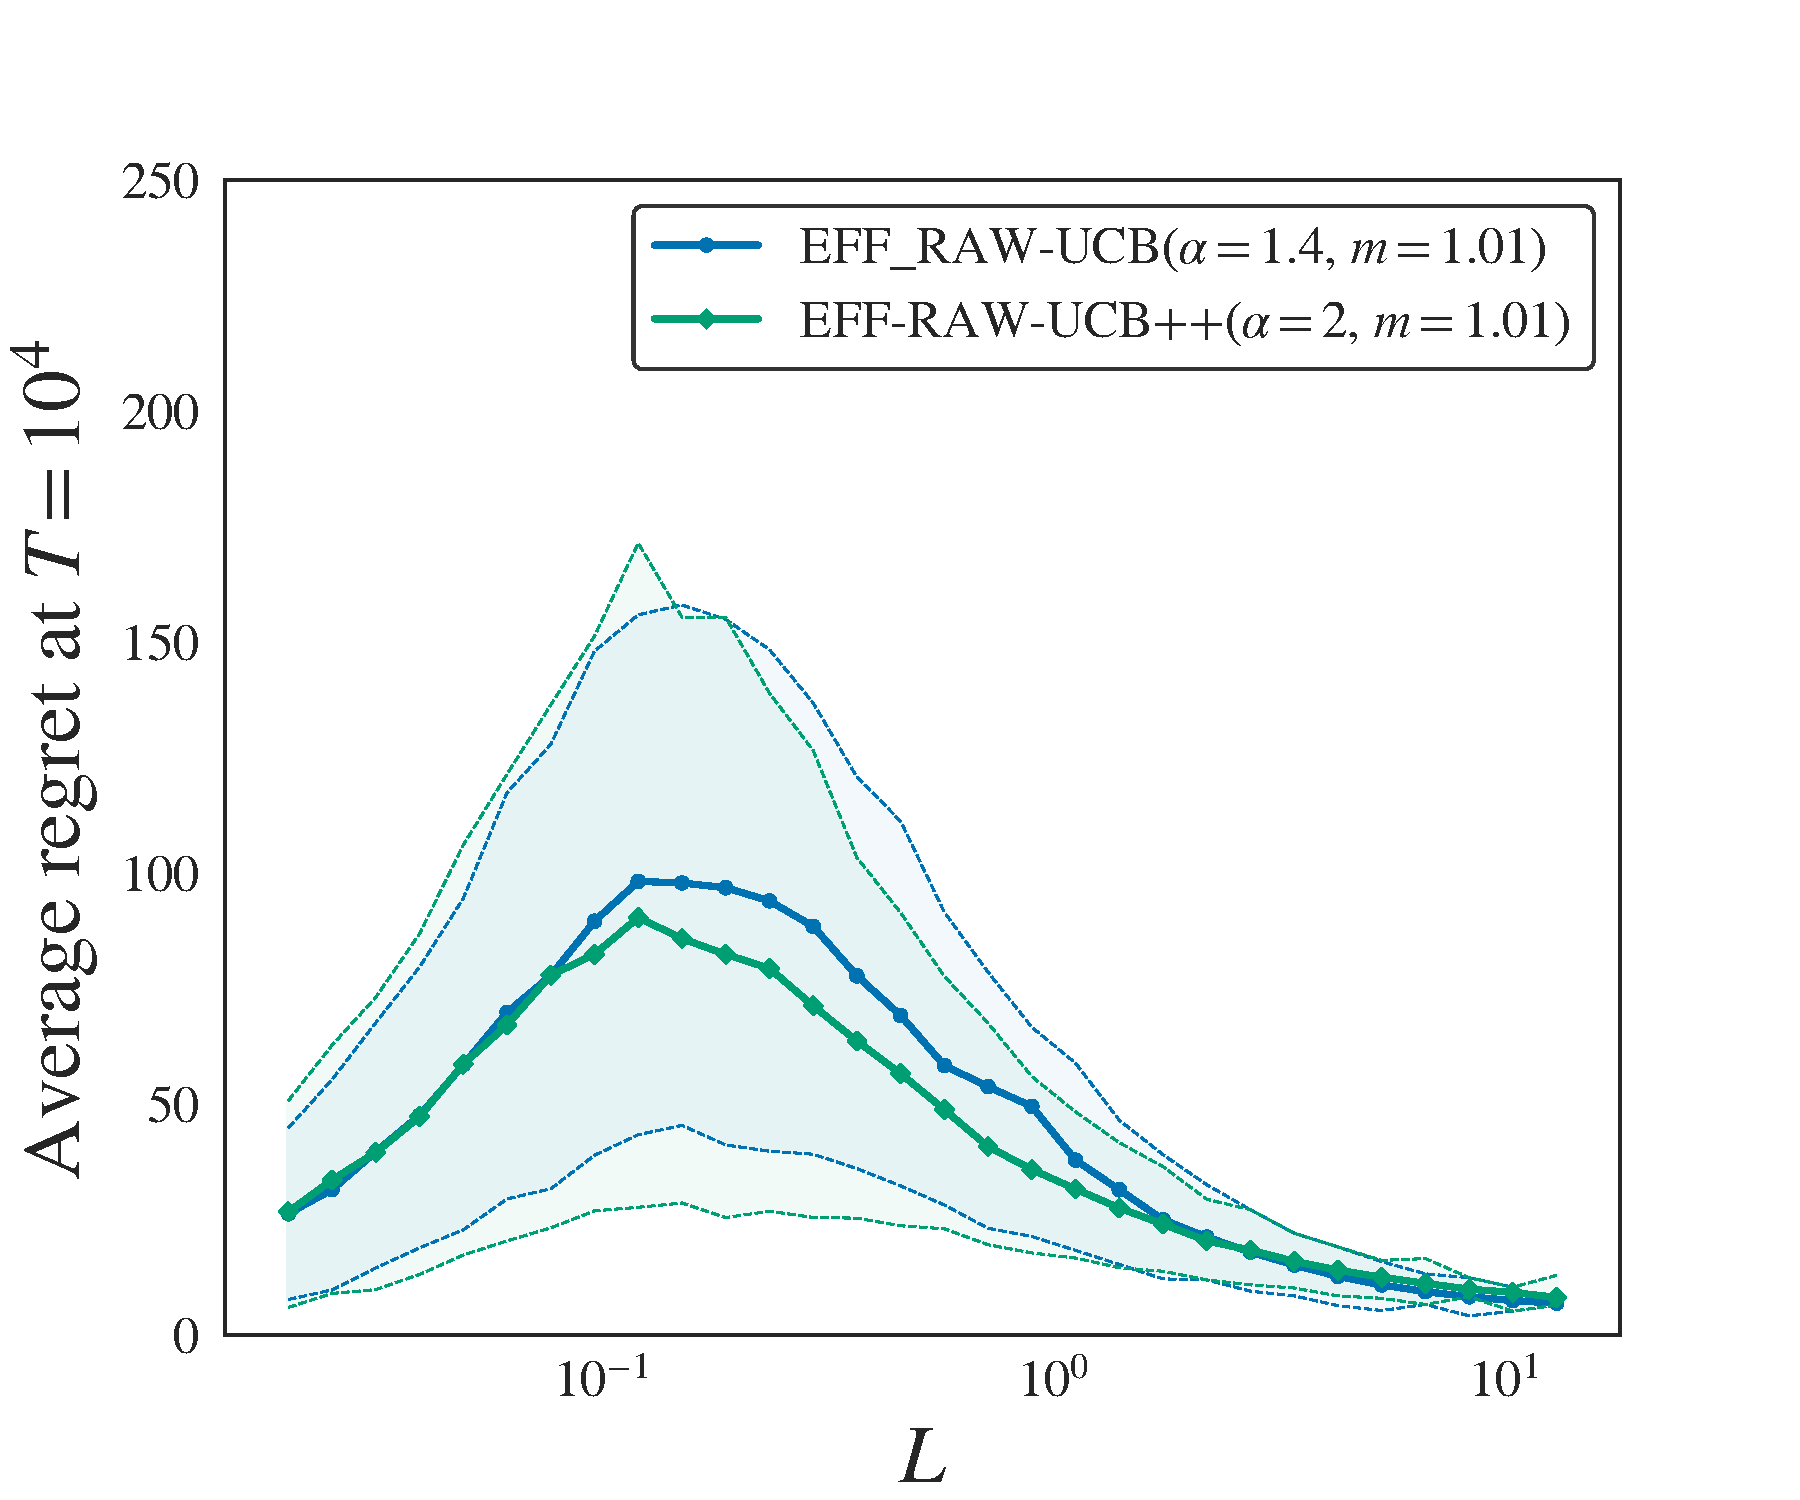
\includegraphics[clip, width= 0.51\textwidth]{2.1Rested/fig/fig1A_pp.pdf}
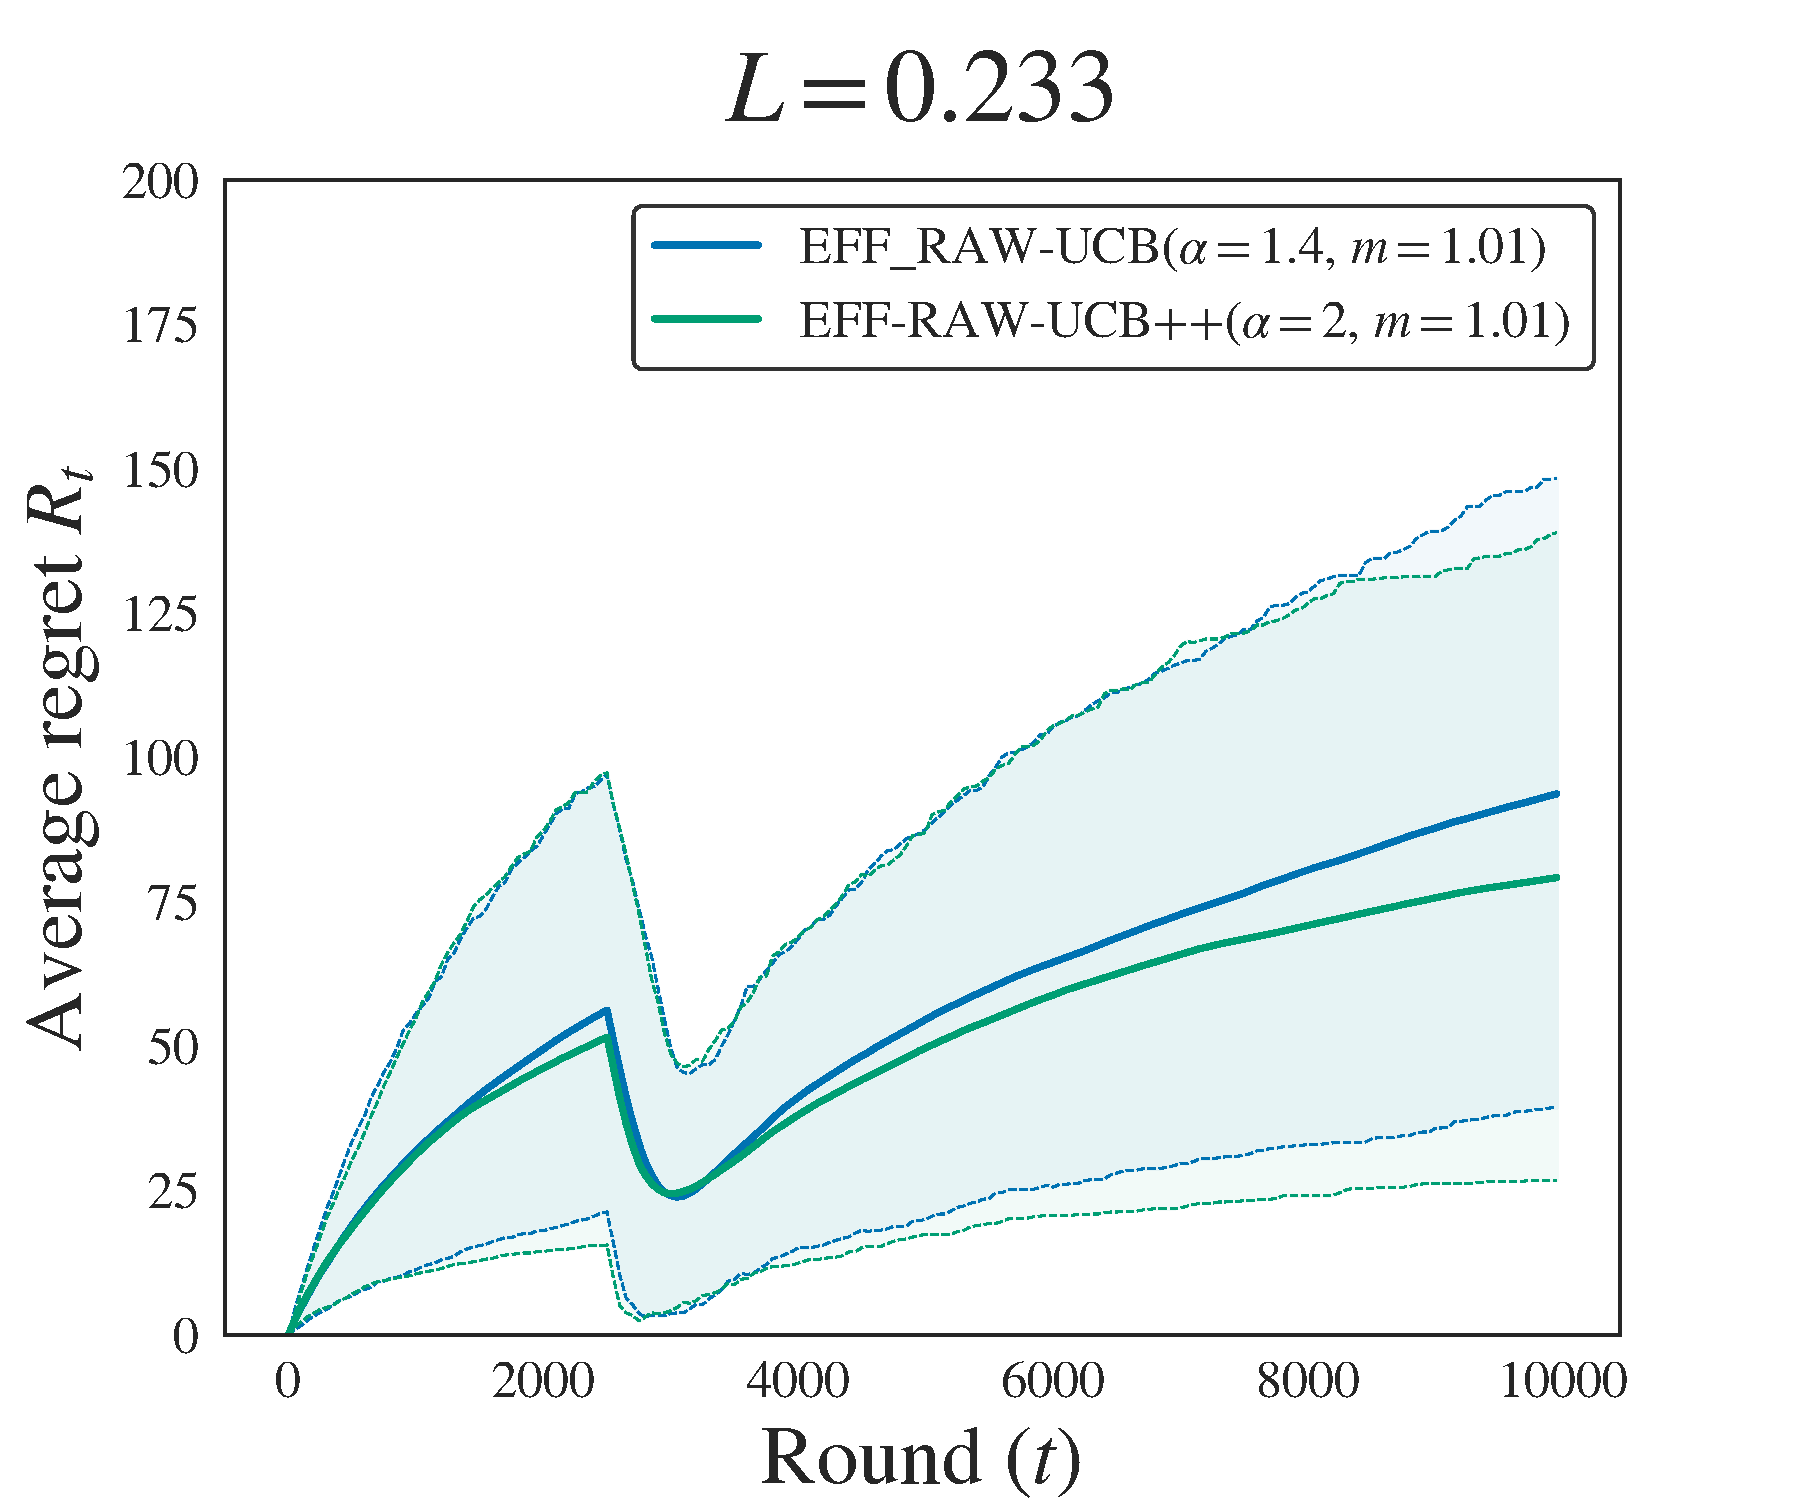
\includegraphics[clip, width= 0.49\textwidth]{2.1Rested/fig/fig1B_pp.pdf}
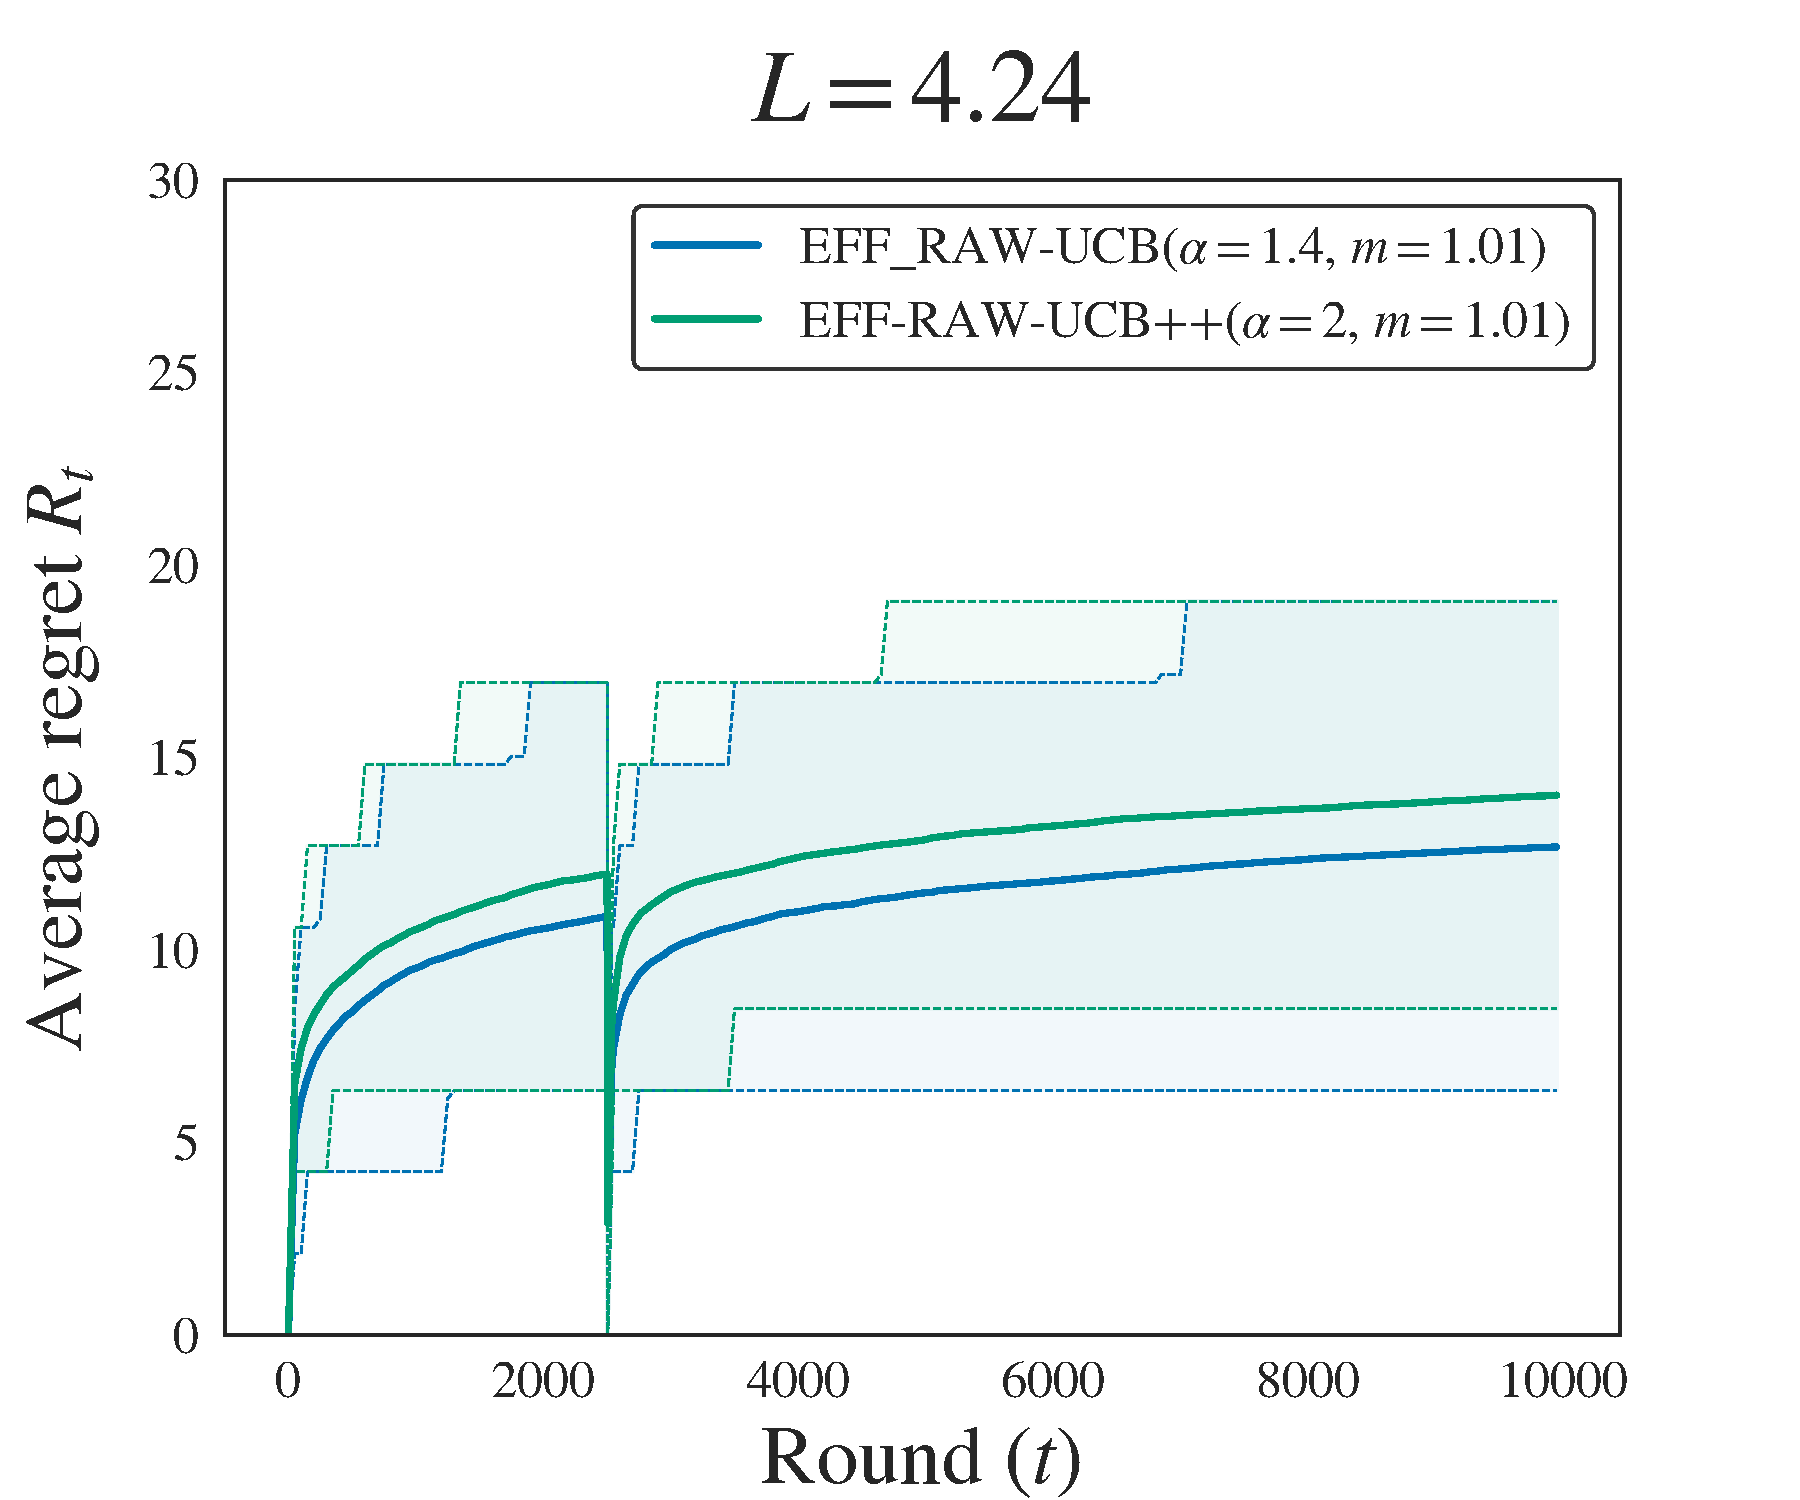
\includegraphics[clip, width= 0.49\textwidth]{2.1Rested/fig/fig1C_pp.pdf}
\caption{\textbf{Top:} Regret at the end of the game for different values of $L$. \textbf{Bottom:} Regret across time for two values of $L$. Average over 1000 runs. We highlight the $\left[10\%, 90\%\right]$ confidence region.}
\label{fig:rested-pp1}
\end{figure*}


\begin{figure*}[ht]
\centering
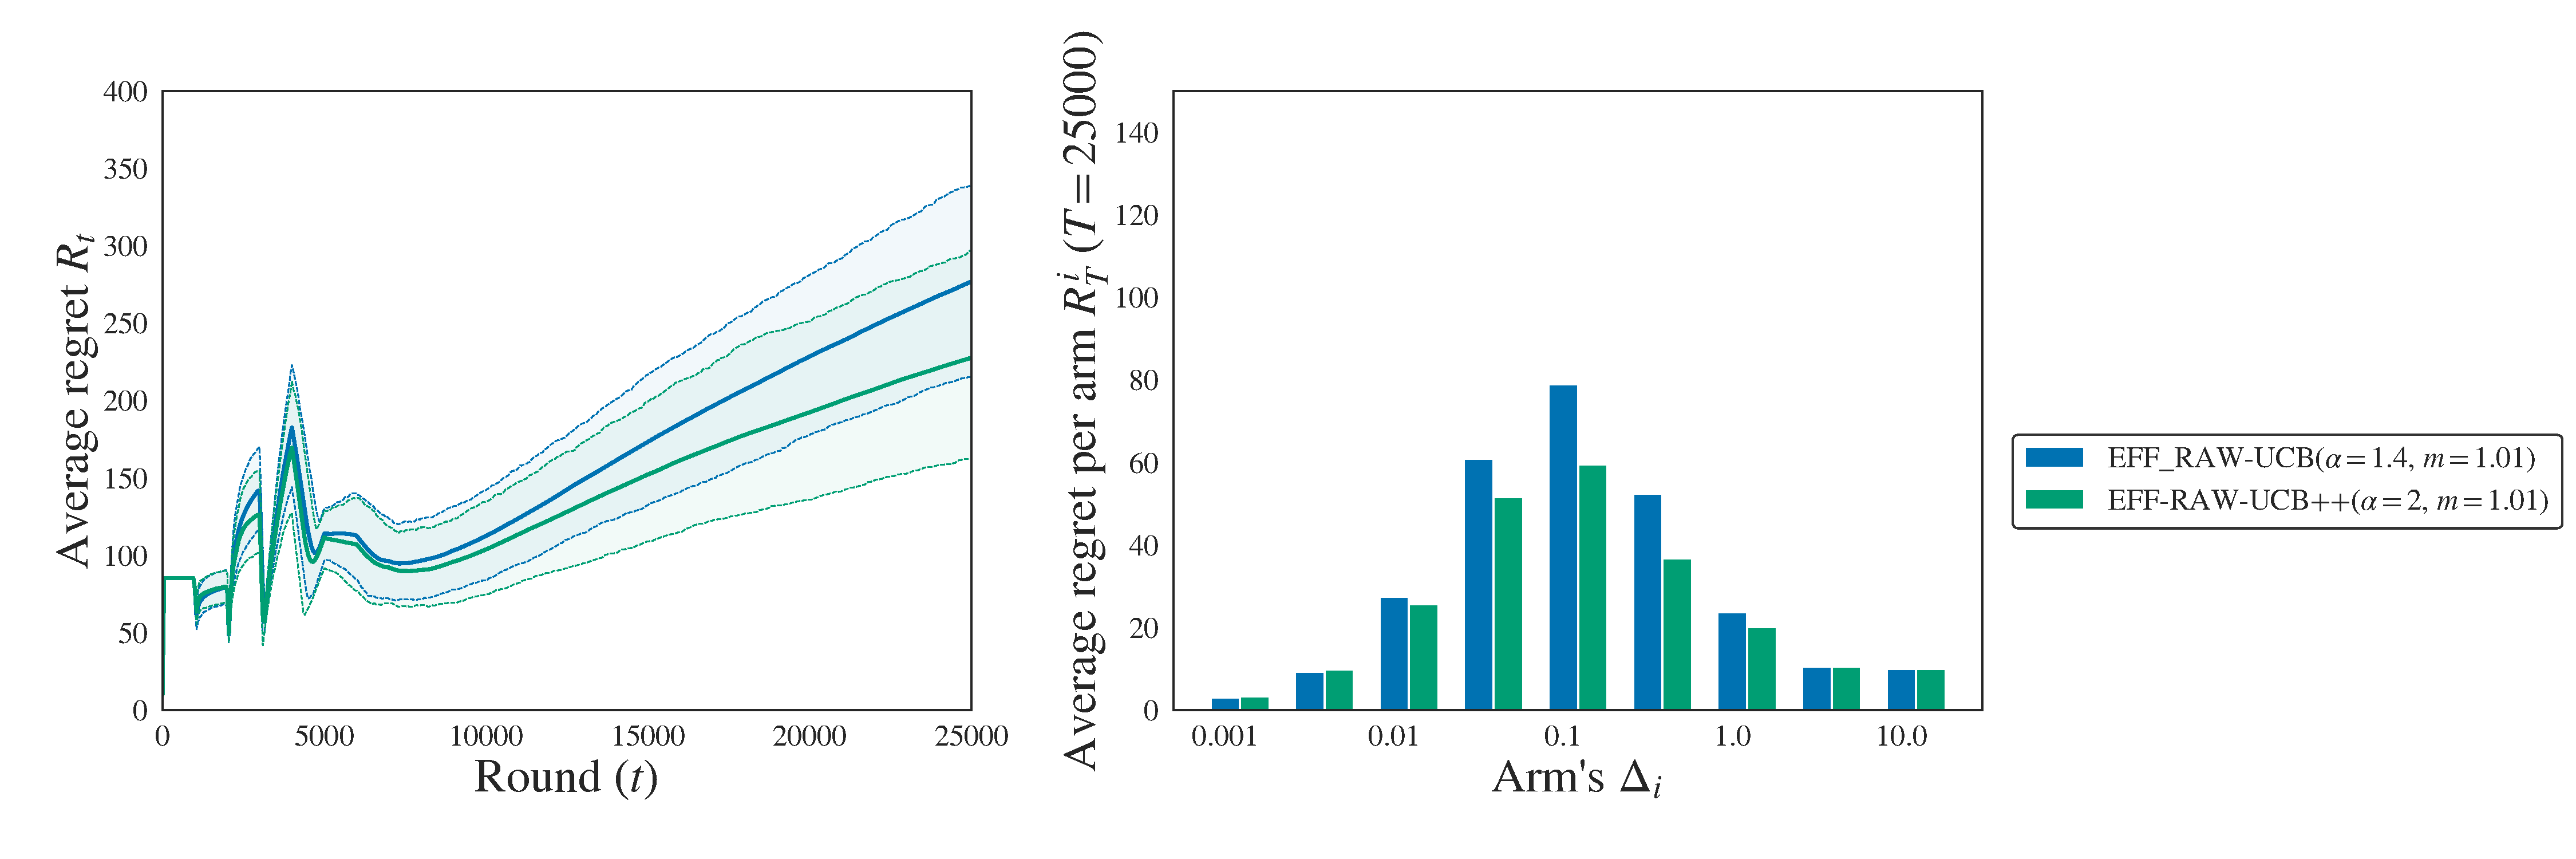
\includegraphics[width = 0.99 \textwidth]{2.1Rested/fig/fig2_pp.pdf}
\caption{\textbf{Left:} Regret at the end of the game for different values of $L$. \textbf{Middle, Right:} Regret across time for two values of $L$. Average over 1000 runs. We highlight the $\left[10\%, 90\%\right]$ confidence region.}
\label{fig:rested-pp2}
\end{figure*}

\subsection{Towards a theoretical analysis of {\RAWUCBpp}}
Analyzing \UCB with tight confidence levels in stationary bandits is already a challenging task \citep{degenne2016anytime, menard2017klucb++, lattimore2018refining}. The analysis of \RAWUCBpp faces two additional difficulties: on the one hand, \RAWUCB 's meta-index is more complex than \UCB 's; on the other hand, rotting bandits are more difficult to analyze than stationary ones. 

First, we can ignore the second part of the problem and try to analyze \RAWUCBpp on stationary problems. Tight analysis of \UCB usually bound the number of pulls of the suboptimal arms. A classical trick is to set a threshold $\mu_\star - \epsilon_i$ and notice that a necessary condition to pull a suboptimal arm $i$ is that either the index of the optimal arm is below the threshold, or the index of the suboptimal arm is above the threshold,

\[ \NiT \leq \sum_{t=1}^T \1 \left[ \texttt{ind}\pa{i_\star, t, \delta_{t,h}} < \mu_\star - \epsilon_i \right] + \1 \left[ \texttt{ind}\pa{i, t, \delta_{t,h}} > \mu_\star - \epsilon_i \right].
\]

The upper deviation of suboptimal arms' indexes is not more difficult to control for \RAWUCB than for \UCB. Indeed, since we take the minimum across confidence bounds, the indexes of \RAWUCB are smaller than the indexes of \UCB (when the confidence levels are the same). 

Controlling the lower deviation of the optimal arm's index is more challenging.  Indeed, at each round $t$, we have to control the probability that any ucb associated with any $h$ last pulls after any $N_{i,t}$ pulls is below the threshold. Compared to \UCB where there is only a scan on the possible values of $N_{i,t}$, we have to handle a double scan on $N_{i,t}$ and $h$. In Section~\ref{sec:theory}, we handle the multiple windows with a crude union bound which leads to a fairly large decrease of the confidence levels. A tighter analysis would probably require better statistical engineering than a union bound or a simple peeling argument. For instance, \citet{maillard2019sequential} develop new concentration results for similar scan statistics for sequential change-point detectors (with some applications to bandits). The difficulty is that the quantity to be bounded is not a sub/super-martingale. Yet, it is quite uncertain that a tighter analysis is actually possible in our case. Indeed, the empirical tuning of \RAWUCB (resp. \RAWUCBpp) increases $\alpha$ by 0.4 (resp. 1) compared to the confidence levels of \UCB (resp. \MOSSa). This is comparable with the theoretical increase of $1$ due to the union bound over all the possible windows.
%!TEX root = ../main.tex 

\section{Linear rotting bandits are impossible to learn}
\label{sec:linear-rotting}
\subsection{Linear bandits}
\label{ss:linear}
In Section~\ref{sec:contextual}, we presented the contextual bandit, a line of work in which the learner is given a context on which depends the action's reward. The linear bandit is a special case where the reward is a noisy linear form of a context-action vector.

Unlike the classical multi-armed bandits, the feedback associated with one action can be used to learn the other actions' efficiency. In fact, the number of actions can be very large or even potentially infinite, as soon as the representation has a finite dimension. 

This shared knowledge is interesting in the context of education. Indeed, a popular model to predict a student's answer is the Item Response Theory \citep{hambleton2013item}. It models the answer with a logistic function filled with a student and question-related parameters. In its most simple form, it can be seen as logistic regression, a generalized linear model. Generalized linear bandits were studied by \citep{filippi2010parametric} as an extension of the linear bandit.  

In the following, we will introduce formally the linear bandit. We will then discuss the possibility of extending our multi-armed rested rotting bandits result in the linear case. 



\subsubsection{Model} At each round, the learner chooses an action $A_t$ in a fixed set of embedded actions $\mathcal{A} \subset \R^d$ and receives,
 \begin{equation*}
\label{eq:linear-feedback}
o_{t} \triangleq \langle \mu | A_t \rangle + \noise_t
 \;\; \text{with}\; \EE{ \noise_t | \historyt }= 0 \;\; \text{and} \; \forall \lambda \in \R, \; \EE{ e^{\lambda\noise_t}} \leq e^{\frac{\subgaussian\lambda^2}{2}},
\end{equation*}
with $\mu \in \R^d$ a reward vector unknown to the learner. In this model, the learner might face a huge number of actions (or even infinite), but they only has $d$ independent parameters to estimate to take the right decision.  The goal of the learner is still to maximize the cumulative reward, 
\begin{equation*}
J_T(\pi) = \sum_{t=1}^T \langle \mu | \pi(t) \rangle. 
\end{equation*}
The optimal oracle strategy selects $\pi^\star(t) = A^\star \triangleq \argmax_{A_t \in \mathcal{A}} \langle \mu | A_t \rangle$. Thus, we can define the regret, 
\[R_T(\pi) = J_T(\pi^\star) - J_T(\pi) = \langle \mu | \sum_{t=1}^T A^\star - \pi(t) \rangle. \]

\subsection{Linear rested rotting bandits}
We want to extend the rested rotting bandit to actions with a linear embedding. We introduce $d$ non-increasing and $L$-Lipschitz functions $\mu_i : \R^+ \rightarrow \R$. While there were $K$ reward functions defined on $\NN$ in the rotting MAB model, we now have $d$ functions defined on $\R^+$. Indeed, we now have $d$ (and not $K$) reward parameters. Moreover, for the rested rotting MAB, the reward is evolving according to the number (in $\NN$) of pulls of arm $i$. In the linear model, we cannot simply count the number of pulls along each direction because $A_t$ has possibly components along all the directions. We will need to find a quantifier of the pulling intensity along direction $i$. This is not surprising that this quantifier will have value in $\R^+$ because we select direction $i$ with intensity $A_{t,i} \in \R$. We suggest using, 
\[
N_{t,i} \triangleq \sum_{t'=1}^t A_{t',i}.
\]

Hence, we define the feedback as, 
\[
o_t = \sum_{i\leq d} \int_{N_{t-1,i}}^{N_{t,i}} \mu_i(x)dx +\noise_t  = \int_{N_{t-1}}^{N_{t}} \langle \mu(n) |   dn \rangle  + \noise_t,
\]
with $\{\noise_t\}$ a sequence of independent $\sigma$-subgaussian random variables. We also define the cumulative reward, 
\[
 J_T(\pi) = \int_{0}^{N_{T}} \langle \mu(n) |  dn \rangle.
 \]

Like in the rotting MAB model, the total reward depends only on the cumulative pulling intensity $N_{T}$. This property is very useful, as it allows to compare the performance of two policies only with their pulling differences (the overpulled/underpulled arms) and not with the specific order of the pulls, \ie, 
\[
 J_T(\pi_2) - J_T(\pi_1) = \int_{N_T^{\pi_1}}^{N_{T}^{\pi_2}} \langle \mu(n) |  dn \rangle.
\]

Last, we restrain the action vector to be in the positive quadrant, \ie $\mathcal{A} \subset \R^{+d}$. Indeed, we want the pulling intensity to be non-decreasing with time $t$ such that the reward associated to a vector $A\in \R^{+d} $ is non-increasing, 

\[
t_1 < t_2 \implies  N_{t_1-1} \leq N_{t_2-1}  \implies \int_{N_{t_1-1}}^{N_{t_1-1} + A} \langle \mu(n) |   dn \rangle \geq \int_{N_{t_2-1}}^{N_{t_2-1} + A} \langle \mu(n) |   dn \rangle.
\]

This model correctly extends linear bandits and rested rotting bandits. On the first hand, when reward functions are constant, we recover the linear bandit model of Subsection~\ref{ss:linear}. Indeed, we have,
\begin{align*}
&o_t =  \int_{N_{t-1}}^{N_{t}} \langle \mu |   dn \rangle  + \noise_t =  \langle \mu | N_t - N_{t-1} \rangle  + \noise_t = \langle \mu | A_t \rangle  + \noise_t,\\
& J_T(\pi) = \int_{0}^{N_{T}} \langle \mu |  dn \rangle = \langle \mu | N_T\rangle =  \sum_{t=1}^T \langle \mu | A_t \rangle .
\end{align*}


On the other hand, when the actions sets $\mathcal{A}$ are the $d$ canonical basis vectors at every round, we recover the rested rotting bandits setting of Section~\ref{sec:rested-model}. Indeed, if we call $\mu_i^{MAB}(n) \triangleq \int_{n}^{n+1} \mu_i(n) dn$, we have,
\begin{align*}
&N_{t,i} = \sum_{t=1}^T \mathbbm{1}(\pi(t) = i),\\
&o_t =  \int_{N_{t-1}}^{N_{t}} \langle \mu(n) |   dn \rangle  + \noise_t = \mu_{i_t}^{MAB}(N_{t-1, i_t}) + \noise_t,\\
& J_T(\pi) = \int_{0}^{N_{T}} \langle \mu(n) |  dn \rangle = \sum_{i\leq d} \sum_{n=0}^{N_{T, i}-1} \mu_{i}^{MAB}(n).
\end{align*}

To conclude the argument, we notice that the constructed functions $\mu_i^{MAB}$ are in $\rewardSet$ (see Definition~\ref{def:rew-bounded-decay}). Indeed, 
\begin{align*}
&\mu_i^{MAB}(n) -\mu_i^{MAB}(n+1) = \int_{n}^{n+1} \pa{\mu_i(x) - \mu_i(x+1)} dx \geq 0,\\
&\mu_i^{MAB}(n) -\mu_i^{MAB}(n+1) = \int_{n}^{n+1} \pa{\mu_i(x) - \mu_i(x+1)} dx \leq L.
\end{align*}
The first line follows by the non-increasing property of $\mu_i$. The second line is justified because $\mu_i$ is $L$-lipschitz.
 
\begin{remark}
We choose to measure the pulling intensity as $N_{t,i} \triangleq \sum_{t'=1}^t A_{t',i}$. In the (stationary) linear bandit problem, the number of pulls is replaced by the matrix $\sum_{t'=1}^t A_{t'}A_{t'}^\intercal$ which is used in the least-square regression and in the confidence ellipsoid computation. Hence, from an information-theoretic point of view, the natural identification is $N_{t,i} \triangleq \sum_{t'=1}^t A_{t',i}^2 $  (which follows when the actions embeddings are the canonical basis vectors). Yet, our choice is motivated because we want a linear dependence between  $N_{t,i}$ and the collected reward along direction $i$ in the stationary case.
\end{remark} 

\subsection{The offline problem}
\label{ss:linear-rotting-offline}
In the rested rotting bandits model, \citet{heidari2016tight} show that the greedy oracle policy which selects the arm with the highest upcoming reward is anytime optimal. Unfortunately, this result does not hold in the linear rotting bandit model. 

\begin{proposition}
\label{prop:linear-rotting-greedy}
Let's consider the simple $d=2$ case. For any horizon $T\geq 2$, there exists an $L$-lipschitz reward vector function $\mu$ bounded in $[0,L]$, a fixed vector arms set $\mathcal{A}$, and a strategy $\pi$ such that the greedy oracle $\GO$ suffers,
\[
J_T(\pi) - J_T(\GO) \geq \frac{L(T-2)}{8}\cdot 
\]
\end{proposition}

We notice that the worst regret for reward values in $[0,L]$ and arms in $[0,1]^d$ is $LT$. Hence, Proposition~\ref{prop:linear-rotting-greedy} shows that $\GO$ is unable to learn as its problem-independent performance is at a constant ratio of the worst possible rate. We will prove precisely this statement in Subsection~\ref{ss:linear-rotting-proofs} but we give here the main intuition. Let's consider a vector reward function such that the first direction decays from $L$ to $0$ in the middle of the game and the second one has a constant reward value $L/2$. In the MAB case - when arms are orthogonal - the greedy oracle $\GO$ stops pulling the first direction when the associated reward decreases. However, when arms are not orthogonal (e.g. $(1,0)$ and $(\nicefrac{1}{2}, \nicefrac{1}{2})$), the greedy policy will collect quickly all the reward associated with the first direction by selecting the first arm. Then, it selects arm $2$ which still pulls a fraction of the first direction, even though the reward has decayed. A better oracle strategy would be to notice that the good reward associated with the first direction will be gathered at the end of the game anyway, and focus on maximizing the reward associated with the other direction.

Notice that this better strategy needs to see at least up to the middle of the game to see that the reward will decay. Otherwise, it will not behave consistently on the problems on which the reward does not decay. Refining this argument, we can show in Proposition~\ref{prop:linear-rotting-short-sighted} that any short-sighted oracle - \ie a policy that can only see the next $T_O$ rewards for any combination of $T_O$ arms - suffers a regret which scales at least with $T-T_O$. It means that the offline problem is a planning problem where we need full knowledge of the reward function and the horizon $T$.

\begin{proposition}
\label{prop:linear-rotting-short-sighted}
Let $\pi$ a short-sighted policy which sees the future rewards associated to any combination of $T_O$ arms. For $T \geq T_O + 23$, there exists a problem $\mu$ and a policy $\pi'$ such that,
\[
J_T(\pi') - J_T(\pi) \geq \frac{L\pa{T-T_O}}{20}\cdot
\]
\end{proposition}

\subsection{The noise-free online problem}
A direct consequence of Proposition~\ref{prop:linear-rotting-short-sighted} is that any learning policy - a special case of short-sighted policies with $T_O =0$ - suffers a worst-case linear regret, even in the absence of noise. Hence, we conclude that the rotting linear setup is not learnable. 
\begin{corollary}
For any learning policy $\pi$ and $T\geq 23$, there exists a problem $\mu$ and a policy $\pi'$
\[
J_T(\pi') - J_T(\pi)  \geq  \frac{LT}{20}\cdot
\]
\end{corollary}

Again, we highlight the deep contrast with the MAB setting, where a simple greedy policy is guaranteed to make at most $K-1$ mistakes. The key argument is that when a direction decreases we need to be able to stop pulling that direction and focus on other directions.  

\subsection{Proofs}
\label{ss:linear-rotting-proofs}
\label{ss:linear-rotting-proof}

\begin{proof}[Proof of Proposition~\ref{prop:linear-rotting-greedy}]
For $d\! =\! 2$, $\mathcal{A} \!=\! \left\{ A_1, A_2 \right\}$ with $A_1 \!=\! (1,0)^\intercal$ and $A_2 \!=\! (\nicefrac{1}{2},\nicefrac{1}{2})^\intercal$. For any horizon $T\geq2$, we consider the following $L$-lipschitz reward functions,
\[
\mu_1(x) = \begin{cases}
L &\text{ if } x < \frac{T-1}{2} \\
L(1- x + \frac{T-1}{2}) &\text{ if }  \frac{T-1}{2} \leq x \leq \frac{T+1}{2}\\
0 &\text{ else}
\end{cases}
\qquad \text{and} \qquad  \mu_2(x) = \frac{L}{2}\cdot
\]

The greedy oracle strategy first selects $A_1$ for $\floor{\frac{T}{2}}$ rounds and then $A_2$ for the remaining $\ceil{\frac{T}{2}}$. Hence,
\begin{align*}
&N_{T,1} = \floor{\frac{T}{2}} + \frac{1}{2} \ceil{\frac{T}{2}}\CommaBin \\
&N_{T,2} = \frac{1}{2} \ceil{\frac{T}{2}} \geq \frac{T+1}{2}\cdot
\end{align*} 
For $T \geq 2$, $N_{T,1} \geq \frac{T+1}{2}$, which means that the greedy policy collects all the $\nicefrac{LT}{2}$ reward along the first direction. We also notice that $N_{T,2} \leq \frac{T+1}{4}$, which means that the total reward is bounded by, 
\[
J_T(\GO) = \int_0^{N_{T,1}} \mu_1(x)dx + \int_0^{N_{T,2}} \mu_2(x)dx  \leq \frac{LT}{2} + \frac{L\pa{T+1}}{8}\cdot
\]
We now consider the policy $\pi_2$ which always selects arm 2. At the end of the game, it gathers the reward,
\[
J_T(\pi_2) = \int_0^{\frac{T}{2}} \mu_1(x)dx + \int_0^{\frac{T}{2}} \mu_2(x)dx = \frac{L\pa{T-\nicefrac{1}{4}} }{2} + \frac{LT}{4}\cdot
\]

Hence, we have that,
\[
J_T(\policy_2) - J_T(\GO) \geq \frac{L(T-2)}{8}\cdot 
\]

\end{proof}

\begin{proof}[Proof of Proposition~\ref{prop:linear-rotting-short-sighted}]
We still consider $d = 2$, $\mathcal{A} = \left\{ A_1, A_2 \right\}$ with $A_1 = (1,0)^\intercal$ and $A_2 = (\nicefrac{1}{2},\nicefrac{1}{2})^\intercal$. For any horizon $T$, we consider the ($L$-lipschitz) two reward vector functions $\mu^1$ and $\mu^2$,
\begin{align*}
&\mu^1_1(x) = L  & \text{and} \;  \mu^1_2(x) = \frac{L}{2} \CommaBin\\
&\mu^2_1(x) = \begin{cases}
L &\text{ if } x <\frac{T+T_O-1}{2} \\
L(1- x +  \frac{T +T_O -1}{2}) &\text{ if }  \frac{T +T_O-1}{2} \leq x \leq \frac{T +T_O+1}{2}\\
0 &\text{ else}
\end{cases}
 & \text{and} \; \mu^2_2(x) = \frac{L}{2}\cdot
\end{align*}

Notice that it is not possible to tell the difference between the two setups for the short-sighted oracle $\pi$ before round $t$ such that $ N_{t,1} \geq \frac{T -T_O -1}{2}$. Notice that this round always exists because $N_{T,1} \geq \frac{T}{2}$ for any policy because the pulling intensity of the first direction is always greater than $\nicefrac{1}{2}$ .

On problem $\mu^1$, we will compare $\pi$ to $\pi_1$ which selects always arm $1$. On problem $\mu^2$, we will compare $\pi$ to $\pi_2$ which selects always arm $2$. We give the cumulative reward of the different policies on the two problems,
\begin{align}
&J^1_T(\pi_1) = LT, \label{eq:linear-J1Tpi1}\\ 
&J^2_T(\pi_2) = \frac{L\pa{T -\nicefrac{1}{4}}}{2} + \frac{LT}{4}\CommaBin\label{eq:linear-J2Tpi2}\\
&J^1_T(\pi) = L\pa{T - N^1_{T,2}}, \label{eq:linear-J1Tpi} \\
&J^2_T(\pi) \leq \frac{L\pa{T + N^2_{T,2}}}{2}\CommaBin\label{eq:linear-J2Tpi}
\end{align}
with $N^k_{T,2}$ the pulling intensity in direction $2$ of $\pi$ on problem $k$. The inequality upper-bounds the reward collected in direction $1$ by its maximum $\nicefrac{LT}{2}$. Since we cannot distinguish between the two problems until $N_{t,1} \geq \frac{T - T_O -1}{2} $, we will show that $N^1_{T,2}$ and $N^2_{T,2}$ are loosely related. 

We call $t_u$ the last round such that the two problems are indistinguishable. Therefore, we have that, 
\[
N_{t_u,1}^1 = N_{t_u,1}^2 \triangleq  N_{t_u,1} \text{ and } N_{t_u,2}^1 = N_{t_u,2}^2\triangleq  N_{t_u,2} .
\]

Problems are indistinguishable until,
\[ N_{t_u,1} < \frac{T - T_O -1}{2} \cdot\]

We also know that the problems can be distinguished at the round $t_u+1$, \ie 
\[  \frac{T - T_O -1}{2} \leq N_{t_u+1,1} \leq N_{t_u,1} +1.\] 

The second inequality is because $N_{t_u+1,1} - N_{t_u,1} \leq \max_{i \leq 2} A_{i,1} = 1$. We have bounded $N_{t_u,1}$ but we use $N_{T,2}^k$  in Equations~\ref{eq:linear-J1Tpi} and~\ref{eq:linear-J2Tpi}. We will start by relating $N_{t_u,2}$ to $N_{t_u,1}$, and then we will relate $N_{T,2}^k$ to $N_{t_u,2}$. We call $n_{t,i}$, the number of pulls of arm $i$ at the round $t$. We have that 
\begin{align*}
&N_{t,1} = n_{t,1} + \frac{n_{t,2}}{2}\CommaBin \\
&N_{t,2} = \frac{n_{t,2}}{2}\CommaBin\\\
&n_{t,1} + n_{t,2} = t.
\end{align*}

We can rewrite $N_{t,1} = t - N_{t,2}$. Hence, the above inequations on $N_{t_u,1}$ can be translated for $N_{t_u,2}$. 
\begin{align}
&N_{t_u,2} > \frac{2t_u - T + T_O+1}{2}\CommaBin \nonumber\\
&N_{t_u,2} \leq \frac{2t_u - T +T_O +3}{2} \cdot\label{eq:ntu2}
\end{align}

We can now bound $N_{t_u,2}^k$ for all $k$,
\[
 \frac{2t_u - T + T_O+1}{2} <N_{t_u,2} \leq N_{T,2} ^k \leq \frac{T-t_u}{2} + N_{t_u,2} \leq \frac{t_u +T_O +3}{2}. 
\]

The first and fourth inequality use Equation~\ref{eq:ntu2}. The second uses that $t_u\leq T$ and that the pulling intensity can only grow through the rounds. The third inequality uses that with $N_{t_u,2}$ pulling intensity at the round $t_u$, the learner cannot reach more than $N_{t_u,2} + \pa{T-t_u} \max_{j}A_{j,2} =N_{t_u,2} + \frac{T-t_u}{2}$ (by selecting arm $2$ until the end of the game).

We can use Equations~\ref{eq:linear-J1Tpi1} and~\ref{eq:linear-J1Tpi} (respectively~\ref{eq:linear-J2Tpi2} and~\ref{eq:linear-J2Tpi}) to lower-bound the difference of performance with respect to policy $\pi_1$ (respectively $\pi_2$) on problem $1$ (respectively $2$). 
\begin{align*}
&J_T^1(\pi_1)- J_T^1(\pi) = LN_{T,2}^1 \geq \frac{L}{2} \pa{2t_u - \pa{T - T_O} +1}\\
&J_T^2(\pi_2)- J_T^2(\pi) \geq  \frac{L}{4} \pa{T - 2N_{T,2}^2- \nicefrac{1}{2}} \geq\frac{L}{4} \pa{T -t_u - T_O - 3.5 } .
\end{align*}

The only quantity which depends on the algorithm $\pi$ is $t_u\in \left\{1, \dots, T\right\}$. In a minimax perspective, we lower bound the maximum of these two bounds,
\[
\max\pa{J_T^1(\pi_1)- J_T^1(\pi), J_T^2(\pi_2)- J_T^2(\pi)} \geq \frac{L\pa{T-T_O}}{10} -1.15L.
\]
We conclude the proof by noticing that when $T-T_O\geq 23$, 
\[
\frac{L\pa{T-T_O}}{10} -1.15L \geq \frac{L\pa{T-T_O}}{20}\cdot
\]
\end{proof}


